%!TEX root = ../thesis_main.tex
%!TEX encoding = UTF-8 Unicode

%%%%%%%%%%%%%%%%%%%%%%%%%%%%%%%%%%%%%%%%%%%%%%%%%%%%%%%%%%%%%%%%%%%%
%%                                                                %%
%%                          PREAMBLE                              %%
%%                                                                %%
%%%%%%%%%%%%%%%%%%%%%%%%%%%%%%%%%%%%%%%%%%%%%%%%%%%%%%%%%%%%%%%%%%%%

%\documentclass[a4paper,twoside,10pt,draft]{memoir} %Compilation rapide
\documentclass[a4paper,twoside,10pt,final]{memoir} %Compilation lente

%!TEX encoding = UTF-8 Unicode
%!TEX root = ../thesis_main.tex


%%%%%%%%%%%%%%%%%%%%%%%%%%%%%%%%%%%%%%%%%%%%%%%%%%%%%%%%%%%%%%%%%%%%
%%                                                                %%
%%                        AUTHOR AND TITLE                        %%
%%                                                                %%
%%%%%%%%%%%%%%%%%%%%%%%%%%%%%%%%%%%%%%%%%%%%%%%%%%%%%%%%%%%%%%%%%%%%

\newcommand{\mytitle}{Robust optimisation of the pathway\texorpdfstring{\\ towards a sustainable whole-energy system}{}}
\newcommand{\mysubtitle}{A hierarchical multi-objective\texorpdfstring{\\ Reinforcement Learning-based approach}{}}
\newcommand{\myauthor}{Xavier Rixhon}

\def\eg{e.g.,\ }
\def\ie{i.e.,\ }
\def\og{``}
\def\fg{''}
\def\deg{$^{circ}$}


\usepackage[record,style=alttreegroup,nomain,symbols]{glossaries-extra}
\glsdisablehyper
%!TEX encoding = UTF-8 Unicode
%!TEX root = ../thesis_main.tex

%%%%%%%%%%%%%%%%%%%%%%%%%%%%%%
%	MATH SYMBOLS							%
%%%%%%%%%%%%%%%%%%%%%%%%%%%%%%

\glsxtrsetgrouptitle{Abreviation}{Abreviation}
\glsxtrsetgrouptitle{Notation}{Notation}

% \newcommand{\sdot}{{\bullet}}
\newcommand{\sdot}{(\cdot)}

% ---------------------------------------------------------------------------- %
% ACRONYMS
%% A

%% P
\newabbreviation[group={Acronyms}]{PCE}{PCE}{Polynomial Chaos Expansion}

%% S
\newabbreviation[group={Acronyms}]{SDGs}{SDGs}{Sustainable Development Goals}

%% U
\newabbreviation[group={Acronyms}]{UQ}{UQ}{Uncertainty Quantification}

% ---------------------------------------------------------------------------- %
% ROMAN
%% A
%\glsxtrnewsymbol[group={rs},description={ith ambient particle}]{ai}{\ensuremath{A_i}}


% ---------------------------------------------------------------------------- %
% GREEK
%\glsxtrnewsymbol[group={gs},description={Yaw angle [$\deg$]}]{beta}{\ensuremath{\beta}}


% ---------------------------------------------------------------------------- %
% Sub- Superscripts
%% A
%\glsxtrnewsymbol[group={ss},description={Relative to the ambient}]{uA}{\ensuremath{\sdot_{A}}}



\renewcommand\glstreegroupheaderfmt[1]{\begingroup\textbf{#1}\vspace{-.2cm}\par\endgroup}
\glsfindwidesttoplevelname
\glsxtrsetgrouptitle{Acronyms}{Acronyms}
\glsxtrsetgrouptitle{rs}{Roman Symbols}
\glsxtrsetgrouptitle{gs}{Greek Symbols}
\glsxtrsetgrouptitle{ss}{Sub- Superscripts}
\glsxtrsetgrouptitle{o}{Operators}

%------------------------
%% A
%\newcommand{\ABL}[2]{$U_\mABL=\SIms{#1}$ - $TI_\mABL={#2}\%$}
%------------------------
%% B

%------------------------
%% C

%------------------------
%% D
\newcommand{\degree}{^\circ}
\newcommand{\dd}{\mathrm{d}}

%------------------------
%% E
\newcommand{\etal}{\textit{et~al.}}
\newcommand{\eg}{e.g.\ }

%------------------------
%% F

%------------------------
%% G

%------------------------
%% H

%------------------------
%% I
\newcommand{\ie}{i.e.\ }

%------------------------
%% K

%------------------------
%% L

%------------------------
%% M

%------------------------
%% N

%------------------------
%% O

%------------------------
%% P

%------------------------
%% Q

%------------------------
%% R

%------------------------
%% S

%------------------------
%% T


%------------------------
%% U
\newcommand{\uh}{\hat{u}}
\newcommand{\uv}{\mathbf{u}} 

\newcommand{\ub}{\boldsymbol{u}} 

\newcommand{\uconvw}{\tilde{U}_W}

%------------------------
%% V
\newcommand{\vv}{\mathbf{v}}
\newcommand{\vb}{\boldsymbol{v}}

%------------------------
%% W
\newcommand{\wv}{\mathbf{w}}
\newcommand{\wb}{\boldsymbol{w}}
\newcommand{\WT}{{\scriptscriptstyle \mathrm{WT}}}

%------------------------
%% X
\newcommand{\xv}{\mathbf{x}}
\newcommand{\xb}{\boldsymbol{x}}

%------------------------
%% Y
\newcommand{\yv}{\mathbf{y}}
\newcommand{\yb}{\boldsymbol{y}}

%------------------------
%% Z
\newcommand{\zv}{\mathbf{z}}
\newcommand{\zb}{\boldsymbol{z}}

%%%%%%%%%%%%%%%%%%%%%%%%%%%%%%
%	OPERATORS 								%
%%%%%%%%%%%%%%%%%%%%%%%%%%%%%%
\newcommand{\der}[2]{\frac{d #1}{d #2}}
\newcommand{\pder}[2]{\frac{\partial #1}{\partial #2}}
\newcommand{\pdern}[3]{\frac{\partial^#3 #1}{\partial #2^#3}}

\newcommand{\avgt}[1]{\left\langle {#1}\right\rangle}
\newcommand{\avgs}[1]{\overline{#1}}

%%%%%%%%%%%%%%%%%%%%%%%%%%%%%%
%	REFERENCES 							%
%%%%%%%%%%%%%%%%%%%%%%%%%%%%%%

\newcommand{\eqqref}[1]{Eq.~\eqref{#1}}
\newcommand{\seqqref}[1]{Eqs.~\eqref{#1}}
\newcommand{\eqqrefs}[2]{Eqs.~\eqref{#1} and \eqref{#2}}
\newcommand{\eqqrefc}[2]{Eqs.~\eqref{#1}, \eqref{#2}}
\newcommand{\eq}[1]{Eq.~\eqref{#1}}
% \newcommand{\eqs}[1]{Eqs.~(\ref{#1})}

\newcommand{\fig}{Fig.~\ref}
\newcommand{\figs}{Figs.~\ref}
\newcommand{\tab}{Table~\ref}
\newcommand{\sect}{Section~\ref}
\newcommand{\chap}{Chapter~\ref}
\newcommand{\chaps}{Chapters~\ref}
\newcommand{\app}{Appendix~\ref}
\newcommand{\apps}{Appendices~\ref}

%%%%%%%%%%%%%%%%%%%%%%%%%%%%%%
%	CAPTIONS							%
%%%%%%%%%%%%%%%%%%%%%%%%%%%%%%
% Color palette
  
\usepackage{xcolor}
\definecolor{myBlue}{rgb}{0.25, 0.25, 0.75}
\definecolor{myRed}{rgb}{0.8, 0.1, 0.3}
\definecolor{myGrey0}{rgb}{0.25, 0.25, 0.25}
\definecolor{myGrey1}{rgb}{0.50, 0.50, 0.50}
\definecolor{myGrey2}{rgb}{0.75, 0.75, 0.75}


\definecolor{Blue0}{rgb}{0.7752402921953095, 0.8583006535947711, 0.9368242983467897}
\definecolor{Blue1}{rgb}{0.41708573625528644, 0.6806305267204922, 0.8382314494425221}
\definecolor{Blue2}{rgb}{0.1271049596309112, 0.4401845444059977, 0.7074971164936563}
\definecolor{Blue3}{rgb}{0.03137254901960784, 0.18823529411764706, 0.4196078431372549}

\definecolor{BluePy}{rgb}{0.69140625, 0.8164, 0.8868}
\definecolor{RedC}{rgb}{0.9453, 0.7266, 0.6602}

\definecolor{gw}{rgb}{1, 0, 0}
\definecolor{jb}{rgb}{0, 1, 0}
\definecolor{tg}{rgb}{0, 0, 1}
\definecolor{jh}{rgb}{1, 1, 0}

\newcommand{\gw}[1]{{#1}}
% \newcoxmmand{\gw}[1]{\textcolor{gw}{#1}}
\newcommand{\jb}[1]{\textcolor{jb}{#1}}
\newcommand{\tg}[1]{\textcolor{tg}{#1}}
\newcommand{\jh}[1]{\textcolor{jh}{#1}}


%%%%%%%%%%%%%%%%%%%%%%%%%%%%%%%%%%%%%%%%%%%%%%%%%%%%%%%%%%%%%%%%%%%%
%%                                                                %%
%%                       LANGUAGE AND FONTS                       %%
%%                                                                %%
%%%%%%%%%%%%%%%%%%%%%%%%%%%%%%%%%%%%%%%%%%%%%%%%%%%%%%%%%%%%%%%%%%%%

% -- Language ------------------------------------------------------
\usepackage[utf8]{inputenc}
\usepackage[USenglish]{babel}
\usepackage[T1]{fontenc} % Accents
\usepackage{scrextend} % to use \footref: multiple reference to the same table footnote
\usepackage{pbox} % to have new line inside table cells

% -- Fonts ---------------------------------------------------------
%\usepackage{lmodern}
%% utopia
%\usepackage{fourier}
%% palatino
%\usepackage{palatino}
%% pifont
%\usepackage{pifont}
%% charter
%\usepackage{charter}

% stix
\usepackage[lcgreekalpha]{stix}
\usepackage{textcomp}

%% better and newer palatino font
%\usepackage{newpxtext,newpxmath}

%% special font, no ams package included...
%\usepackage[full]{textcomp}
%\usepackage[osf]{newtxtext} % osf for text, not math
%\usepackage{cabin} % sans serif
%\usepackage[varqu,varl]{inconsolata} % sans serif typewriter
%\usepackage[bigdelims,vvarbb]{newtxmath} % bb from STIX
%\usepackage[cal=boondoxo]{mathalfa} % mathcal


%%%%%%%%%%%%%%%%%%%%%%%%%%%%%%%%%%%%%%%%%%%%%%%%%%%%%%%%%%%%%%%%%%%%
%%                                                                %%
%%                    TEXT, LAYOUT AND STRUCTURE                  %%
%%                                                                %%
%%%%%%%%%%%%%%%%%%%%%%%%%%%%%%%%%%%%%%%%%%%%%%%%%%%%%%%%%%%%%%%%%%%%

% -- Paragraphs---- ------------------------------------------------
\linespread{1.15}
%\usepackage[parfill]{parskip} %% NOT working with memoir class... see https://tex.stackexchange.com/questions/193485/how-to-use-usepackageparfillparskip-in-memoir-class for discussion

% -- Margins -------------------------------------------------------
\usepackage[includehead,includefoot,centering,height=20cm,width=12cm,showframe=false]{geometry}
%\usepackage[includehead,includefoot,centering,height=20cm,width=12cm,showframe=false]{geometry}

%\usepackage[includehead,includefoot,centering,height=20cm,width=12cm,showframe=true]{geometry} %taille des marges
%\usepackage[includehead, includefoot, top=4.2cm, bottom=5.4cm, left=4.5cm, right=4.5cm,showframe=true]{geometry}%…PhP
%\usepackage[includehead, includefoot, top=4.8cm, bottom=4.8cm, left=4.5cm, right=4.5cm,showframe=true]{geometry}%4.8 4.8

% -- Layout --------------------------------------------------------
%\usepackage{layout} % pour afficher le layout des pages

%\usepackage{color}
%\usepackage[dvipsnames]{xcolor}s
\usepackage{lineno}
%\usepackage{ulem} %underline for emphasis
\usepackage{fancyhdr}% pour en-tetes personnalises
\usepackage{appendix} % gestion appendix
\usepackage{tikz}% pour diagrammes
\usetikzlibrary{shapes.misc}
\usepackage{setspace}

%\usepackage{titlepages} % for the titlepage examples

%\usepackage{charter}
%\usepackage[raggedright]{titlesec} % evite les coupures de mot dans les titres

\usepackage{afterpage} % Force content to be on the next page

%% The lineno packages adds line numbers. Start line numbering with
%% \begin{linenumbers}, end it with \end{linenumbers}. Or switch it on
%% for the whole article with \linenumbers.
\usepackage{lineno} % Line numbers

\sloppy % evite les debordements de texte dans la marge
\raggedbottom %regroupe les espaces verticaux automatiques au bas des pages

% -- Structure et Paragraphes --------------------------------------
%evite les lignes veuves et orphelines
\clubpenalty=10000
\widowpenalty=10000
\interfootnotelinepenalty=10000

%\setcounter{secnumdepth}{3} % numerote les subsubsections
\setsecnumdepth{subsection}
\maxtocdepth{subsection}

% -- Style ---------------------------------------------------------
\normalfont
% chapter style
%\chapterstyle{ell}
%\chapterstyle{madsen}
%\chapterstyle{bianchi}
%\chapterstyle{dash}
%\chapterstyle{thatcher}
\newcommand{\clearemptydoublepage}{\newpage{\pagestyle{empty}\cleardoublepage}} %pour effacer les en-tetes sur la page vierge avant chaque chapitre

%\pagestyle{ruled}
\nouppercaseheads
\pagestyle{headings}
\makeheadrule{headings}{\textwidth}{0.3pt}


%%%%%%%%%%%%%%%%%%%%%%%%%%%%%%%%%%%%%%%%%%%%%%%%%%%%%%%%%%%%%%%%%%%%
%%                                                                %%
%%                     TABLES AND FIGURES                         %%
%%                                                                %%
%%%%%%%%%%%%%%%%%%%%%%%%%%%%%%%%%%%%%%%%%%%%%%%%%%%%%%%%%%%%%%%%%%%%

% -- Figures -------------------------------------------------------
\usepackage{graphicx}
\graphicspath{{frontend/img/}{chap_intro_ccl/img/}{chap_case_study/img/}{chap_ES_PCE/img/}{chap_electro_uq/img/}{chap_methodo/img/}{chap_myopic/img/}{chap_RL/img/}{chap_atom_mol/img/}{chap_RobPol/img/}{appendices/img/}} % Figures folder different for each input
%\graphicspath{{img/}} %
\DeclareGraphicsExtensions{.eps,.pdf,.png,.jpg}

%\usepackage[cleanup,process=auto]{pstool}
%\usepackage[cleanup,process=all]{pstool} % force process every figure
%\usepackage{pst-pdf}
%\usepackage{epstopdf}
%\usepackage{auto-pst-pdf} 
%\usepackage{psfrag}
%\PassOptionsToPackage{psfrag}{process=none}

\usepackage[figuresright]{rotating} %https://tex.stackexchange.com/questions/337/how-to-change-certain-pages-into-landscape-portrait-mode

\def\figwidth{0.9\textwidth}
\newcommand{\singlefigwidth}{.75\textwidth}

\setfloatadjustment{figure}{\centering}
\setfloatlocations{figure}{thb}
\newsubfloat{figure}

\newcommand{\illusname}{Illustration}
\newcommand{\listillusname}{List of Illustrations}
\newlistof{listofillus}{loillu}{\listdiagramname}
\newfloat[chapter]{illustration}{loillu}{\illusname}
\newlistentry{illustration}{loillu}{0}
\renewcommand\theillustration{\arabic{illustration}}    

\usetikzlibrary{shapes}

% -- Tables --------------------------------------------------------
\usepackage{booktabs} % Table customization: \specialrule

\usepackage{longtable} % Long tables on multiple pages
\usepackage{tabu}
\usepackage{ltablex} % Use ltablex instead of tabularx
\usepackage{multirow} % Cellule de tableau sur plusieurs lignes
\usepackage{multicol} % Cellule de tableau sur plusieurs colonnes
\usepackage{dcolumn} % Columns aligned on decimal point
\newcolumntype{d}[1]{D{.}{.}{#1}}
\usepackage{array} % ??

%\usepackage{cellspace} % Espace entre le texte et les bord des cellules
%\usepackage{tabularx} % Tableau avec largeur fixée

\usepackage{makecell} % Customize table headers with \thead
\renewcommand\theadfont{\bfseries} % Customize table column headers with \thead

% -- Sub-figures and Captions --------------------------------------
\usepackage{subfig}
\usepackage{wrapfig} % Images dans le texte
%\usepackage{floatrow} % Tableau et figure côte à côte
%\usepackage{subcaption} % sub caption

\usepackage[labelfont=bf, labelsep=period, justification=justified,singlelinecheck=false]{caption} % style et taille de police des captions
%\captionsetup[table]{position=below}

%\captionnamefont{\sffamily} % font for the "Figure xx" part
%\captionnamefont{\footnotesize\sffamily} % font for the "Figure xx" part
%\captionnamefont{\footnotesize} % font for the "Figure xx" part
%\captiontitlefont{\footnotesize} % font for the caption part
%\captiontitlefont{\small}
% change caption witdth
%\changecaptionwidth
%\captionwidth{0.9\textwidth}
%\captionstyle[\centering]{}


%%%%%%%%%%%%%%%%%%%%%%%%%%%%%%%%%%%%%%%%%%%%%%%%%%%%%%%%%%%%%%%%%%%%
%%                                                                %%
%%                      SCIENTIFIC PACKAGES                       %%
%%                                                                %%
%%%%%%%%%%%%%%%%%%%%%%%%%%%%%%%%%%%%%%%%%%%%%%%%%%%%%%%%%%%%%%%%%%%%

% -- Math ----------------------------------------------------------
\usepackage{amsmath}
%\usepackage[intlimits]{amsmath}
\usepackage{amsfonts}
\usepackage{amsthm} % Extended theorem environments
%\usepackage{amssymb} % Math symbols %%redundant with stix package
%\usepackage{esint} % Intégrales multiples
%\usepackage{esvect} % Vecteurs
\usepackage{mathtools}
\usepackage{pifont}

% Put the equation label in the document, to help writing
\usepackage{showlabels}
%\usepackage[final]{showlabels} %disable

\usepackage[boxed]{algorithm2e}

% -- Physics and Chemistry -----------------------------------------
\usepackage{siunitx} % SI units
\usepackage[version=4]{mhchem} % Chemical equations

% -- Symbols -------------------------------------------------------
\usepackage[super]{nth} %text superscript \nth{i}
\usepackage{textcomp} % Degree symbol °, and certainly others
%\newcommand{\cmark}{\ding{51}}
%\newcommand{\xmark}{\ding{55}}


%%%%%%%%%%%%%%%%%%%%%%%%%%%%%%%%%%%%%%%%%%%%%%%%%%%%%%%%%%%%%%%%%%%%
%%                                                                %%
%%                  BIBLIOGRAPHY AND HYPERREF                     %%
%%                                                                %%
%%%%%%%%%%%%%%%%%%%%%%%%%%%%%%%%%%%%%%%%%%%%%%%%%%%%%%%%%%%%%%%%%%%%

% -- Bibliography --------------------------------------------------
% For natbib help, see http://merkel.texture.rocks/Latex/natbib.php?lang=fr
%\usepackage{biblatex}
\usepackage[square,numbers,sort&compress]{natbib}
%\setlength{\bibsep}{0.5pt}
%\usepackage{pdfcomment}
%\usepackage[square,numbers,compress]{natbibtooltip}
\usepackage{textcomp} % recognize the textquotesingle from bib

\bibliographystyle{options/elsarticle-num-names}  %Ordered by appearance in the text, with DOI and URL

%\bibliographystyle{options/elsarticle-num}  %Same but \citet command does not work
%\bibliographystyle{options/elsarticle-harv}  %Harvard style (Author, year, no number)
%\bibliographystyle{options/elsarticle-num-names-nourldoi}  %Ordered by appearance in the text, with DOI
%\bibliographystyle{options/elsarticle-names-nourldoi}  %Ordered by alphabet, with DOI
%\bibliographystyle{options/elsarticle-names-nourl} %Ordered by alphabet, without DOI
%\bibliographystyle{options/model4-names}

% -- Hyperref ------------------------------------------------------
\PassOptionsToPackage{hyphens}{url} %this helps breaking URL when too long
\usepackage[bookmarks,hidelinks]{hyperref}
\usepackage{cleveref}
\usepackage{bm} % To use \bm in order to get bold math symbols

% PDF metadata
\hypersetup{pdftitle={\mytitle}}
\hypersetup{pdfauthor={\myauthor}}
\hypersetup{pdfsubject={PhD thesis}}
\hypersetup{pdfkeywords={Energy System Modelling,EnergyScope,Reinforcement Learning,Policy Optimisation, Electro-fuels}}

% Links color
\newcommand\myshade{85}
% from http://latexcolor.com
\definecolor{airforceblue}{rgb}{0.36, 0.54, 0.66}
\definecolor{battleshipgrey}{rgb}{0.52, 0.52, 0.51}
\definecolor{burntumber}{rgb}{0.54, 0.2, 0.14}
\definecolor{sangria}{rgb}{0.57, 0.0, 0.04}
\colorlet{mylinkcolor}{sangria}
\colorlet{mycitecolor}{battleshipgrey}

%\hypersetup{
%%linkcolor  = mylinkcolor!\myshade!black,
%%citecolor  = mycitecolor!\myshade!black,
%%urlcolor   = myurlcolor!\myshade!black,
%colorlinks = true,
%}

%\hypersetup{
%    colorlinks=true,
%    citecolor = blue,
%    linkcolor=blue,
%    urlcolor = blue
% }

%% Links with color frame
\hypersetup{
colorlinks = false,
%citebordercolor ={red},
}

%% No color on links (for printing)
%\hypersetup{hidelinks}

% Adding bookmarks to pdf (works after clearing aux and then 2 clean compilations)
%\hypersetup{bookmarks={true}} % --> does it by default

%% Reference with Fancy Tooltips (only works with the dedicated compilation script)
%from: https://tex.stackexchange.com/questions/84681/interactive-pdf-latex-and-article-of-the-future/84700#84700
%\usepackage[inactive,blur=0.6, fixcolor]{fancytooltips}
%\usepackage[inactive]{fancytooltips}

% -- Footnotes ------------------------------------------------------
\newcommand\blfootnote[1]{%
  \begingroup
  \renewcommand\thefootnote{}\footnote{#1}%
  \addtocounter{footnote}{-1}%
  \endgroup} %%Footnotes sans numéro

%%!TEX encoding = UTF-8 Unicode
%!TEX root = ../thesis_main.tex

%%%%%%%%%%%%%%%%%%%%%%%%%%%%%%
%	MATH SYMBOLS							%
%%%%%%%%%%%%%%%%%%%%%%%%%%%%%%

\glsxtrsetgrouptitle{Abreviation}{Abreviation}
\glsxtrsetgrouptitle{Notation}{Notation}

% \newcommand{\sdot}{{\bullet}}
\newcommand{\sdot}{(\cdot)}

% ---------------------------------------------------------------------------- %
% ACRONYMS
%% A

%% P
\newabbreviation[group={Acronyms}]{PCE}{PCE}{Polynomial Chaos Expansion}

%% S
\newabbreviation[group={Acronyms}]{SDGs}{SDGs}{Sustainable Development Goals}

%% U
\newabbreviation[group={Acronyms}]{UQ}{UQ}{Uncertainty Quantification}

% ---------------------------------------------------------------------------- %
% ROMAN
%% A
%\glsxtrnewsymbol[group={rs},description={ith ambient particle}]{ai}{\ensuremath{A_i}}


% ---------------------------------------------------------------------------- %
% GREEK
%\glsxtrnewsymbol[group={gs},description={Yaw angle [$\deg$]}]{beta}{\ensuremath{\beta}}


% ---------------------------------------------------------------------------- %
% Sub- Superscripts
%% A
%\glsxtrnewsymbol[group={ss},description={Relative to the ambient}]{uA}{\ensuremath{\sdot_{A}}}



\renewcommand\glstreegroupheaderfmt[1]{\begingroup\textbf{#1}\vspace{-.2cm}\par\endgroup}
\glsfindwidesttoplevelname
\glsxtrsetgrouptitle{Acronyms}{Acronyms}
\glsxtrsetgrouptitle{rs}{Roman Symbols}
\glsxtrsetgrouptitle{gs}{Greek Symbols}
\glsxtrsetgrouptitle{ss}{Sub- Superscripts}
\glsxtrsetgrouptitle{o}{Operators}

%------------------------
%% A
%\newcommand{\ABL}[2]{$U_\mABL=\SIms{#1}$ - $TI_\mABL={#2}\%$}
%------------------------
%% B

%------------------------
%% C

%------------------------
%% D
\newcommand{\degree}{^\circ}
\newcommand{\dd}{\mathrm{d}}

%------------------------
%% E
\newcommand{\etal}{\textit{et~al.}}
\newcommand{\eg}{e.g.\ }

%------------------------
%% F

%------------------------
%% G

%------------------------
%% H

%------------------------
%% I
\newcommand{\ie}{i.e.\ }

%------------------------
%% K

%------------------------
%% L

%------------------------
%% M

%------------------------
%% N

%------------------------
%% O

%------------------------
%% P

%------------------------
%% Q

%------------------------
%% R

%------------------------
%% S

%------------------------
%% T


%------------------------
%% U
\newcommand{\uh}{\hat{u}}
\newcommand{\uv}{\mathbf{u}} 

\newcommand{\ub}{\boldsymbol{u}} 

\newcommand{\uconvw}{\tilde{U}_W}

%------------------------
%% V
\newcommand{\vv}{\mathbf{v}}
\newcommand{\vb}{\boldsymbol{v}}

%------------------------
%% W
\newcommand{\wv}{\mathbf{w}}
\newcommand{\wb}{\boldsymbol{w}}
\newcommand{\WT}{{\scriptscriptstyle \mathrm{WT}}}

%------------------------
%% X
\newcommand{\xv}{\mathbf{x}}
\newcommand{\xb}{\boldsymbol{x}}

%------------------------
%% Y
\newcommand{\yv}{\mathbf{y}}
\newcommand{\yb}{\boldsymbol{y}}

%------------------------
%% Z
\newcommand{\zv}{\mathbf{z}}
\newcommand{\zb}{\boldsymbol{z}}

%%%%%%%%%%%%%%%%%%%%%%%%%%%%%%
%	OPERATORS 								%
%%%%%%%%%%%%%%%%%%%%%%%%%%%%%%
\newcommand{\der}[2]{\frac{d #1}{d #2}}
\newcommand{\pder}[2]{\frac{\partial #1}{\partial #2}}
\newcommand{\pdern}[3]{\frac{\partial^#3 #1}{\partial #2^#3}}

\newcommand{\avgt}[1]{\left\langle {#1}\right\rangle}
\newcommand{\avgs}[1]{\overline{#1}}

%%%%%%%%%%%%%%%%%%%%%%%%%%%%%%
%	REFERENCES 							%
%%%%%%%%%%%%%%%%%%%%%%%%%%%%%%

\newcommand{\eqqref}[1]{Eq.~\eqref{#1}}
\newcommand{\seqqref}[1]{Eqs.~\eqref{#1}}
\newcommand{\eqqrefs}[2]{Eqs.~\eqref{#1} and \eqref{#2}}
\newcommand{\eqqrefc}[2]{Eqs.~\eqref{#1}, \eqref{#2}}
\newcommand{\eq}[1]{Eq.~\eqref{#1}}
% \newcommand{\eqs}[1]{Eqs.~(\ref{#1})}

\newcommand{\fig}{Fig.~\ref}
\newcommand{\figs}{Figs.~\ref}
\newcommand{\tab}{Table~\ref}
\newcommand{\sect}{Section~\ref}
\newcommand{\chap}{Chapter~\ref}
\newcommand{\chaps}{Chapters~\ref}
\newcommand{\app}{Appendix~\ref}
\newcommand{\apps}{Appendices~\ref}

%%%%%%%%%%%%%%%%%%%%%%%%%%%%%%
%	CAPTIONS							%
%%%%%%%%%%%%%%%%%%%%%%%%%%%%%%
% Color palette
  
\usepackage{xcolor}
\definecolor{myBlue}{rgb}{0.25, 0.25, 0.75}
\definecolor{myRed}{rgb}{0.8, 0.1, 0.3}
\definecolor{myGrey0}{rgb}{0.25, 0.25, 0.25}
\definecolor{myGrey1}{rgb}{0.50, 0.50, 0.50}
\definecolor{myGrey2}{rgb}{0.75, 0.75, 0.75}


\definecolor{Blue0}{rgb}{0.7752402921953095, 0.8583006535947711, 0.9368242983467897}
\definecolor{Blue1}{rgb}{0.41708573625528644, 0.6806305267204922, 0.8382314494425221}
\definecolor{Blue2}{rgb}{0.1271049596309112, 0.4401845444059977, 0.7074971164936563}
\definecolor{Blue3}{rgb}{0.03137254901960784, 0.18823529411764706, 0.4196078431372549}

\definecolor{BluePy}{rgb}{0.69140625, 0.8164, 0.8868}
\definecolor{RedC}{rgb}{0.9453, 0.7266, 0.6602}

\definecolor{gw}{rgb}{1, 0, 0}
\definecolor{jb}{rgb}{0, 1, 0}
\definecolor{tg}{rgb}{0, 0, 1}
\definecolor{jh}{rgb}{1, 1, 0}

\newcommand{\gw}[1]{{#1}}
% \newcoxmmand{\gw}[1]{\textcolor{gw}{#1}}
\newcommand{\jb}[1]{\textcolor{jb}{#1}}
\newcommand{\tg}[1]{\textcolor{tg}{#1}}
\newcommand{\jh}[1]{\textcolor{jh}{#1}}


\begin{document}


%%%%%%%%%%%%%%%%%%%%%%%%%%%%%%%%%%%%%%%%%%%%%%%%%%%%%%%%%%%%%%%%%%%%
%%                                                                %%
%%                       FRONT MATTER                             %%
%%                                                                %%
%%%%%%%%%%%%%%%%%%%%%%%%%%%%%%%%%%%%%%%%%%%%%%%%%%%%%%%%%%%%%%%%%%%%

%!TEX encoding = UTF-8 Unicode 
%!TEX root = ../thesis_main.tex
\begin{titlingpage}

\begin{figure}[!t]
\begin{minipage}[m]{.46\textwidth}
\flushleft

\includegraphics[width=\textwidth]{UCL_immc.pdf}
\end{minipage}
\hfill
\begin{minipage}[m]{.40\textwidth}
\flushright
\vspace{-0.25cm}

\includegraphics[width=\textwidth]{BEST_SPF.pdf}
\end{minipage}
\vspace{3 cm}
\end{figure}

\vspace{2 cm}

%\begin{flushleft}
%\rule[-0,2 cm]{\textwidth}{1mm}
%\end{flushleft}

\begin{flushright}
\vspace{0.2cm}
{\fontsize{16}{20}\selectfont \mytitle\\[1em]
{\fontsize{14}{16}\selectfont \mysubtitle}}
\end{flushright}

\begin{flushright}
%\begin{center}
\rule{0.75\linewidth}{0.2mm}
%\end{center}
\end{flushright}

\begin{flushright}
\vspace{1 cm}
\begin{small}
Doctoral dissertation presented by\\
\vspace{0.1cm}
{\Large \textbf{Xavier \textsc{Rixhon}}}\\
\vspace{0.1cm}
%Ingénieur,\\
in partial fulfillment of the requirements for\\
the degree of Doctor in Engineering Sciences\\[1em]%
\end{small}
\end{flushright}

\begin{flushright}
\begin{small}
September 2024\\%
\end{small}
%\vspace{0.5 cm}
\end{flushright}


\vspace{\fill}
%\centering
\begin{small}
%\resizebox{\linewidth}{!}{
\begin{tabular}{l}
%\toprule
%\multicolumn{1}{l}{\textbf{Composition du jury}}\\
\textbf{Thesis committee}\\
%\toprule
\selectfont
Pr. Francesco \textsc{Contino} (UCLouvain, Supervisor) \\ 
Pr. Hervé \textsc{Jeanmart} (UCLouvain, Supervisor) \\ 
Pr. Paul \textsc{Fisette} (UCLouvain, President) \\ 
Pr. Christophe \textsc{De Vleeschouwer} (UCLouvain, Secretary) \\ 
Pr. Sylvain \textsc{Quoilin} (ULiège) \\
Dr. Stefano \textsc{Moret} (ETH Zurich)\\
Pr. Stefan \textsc{Pfenninger} (TU Delft)\\

%\bottomrule
% mettre par ordre alphabétique 
\end{tabular} 
%}
\end{small}
%
\clearpage
%\thispagestyle{empty}
\vspace*{\fill}{\center{
\copyright \hspace{0.1cm} 2023\\
Xavier Rixhon\\
All Rights Reserved\\}}

\end{titlingpage}





\frontmatter

%% -- Abstract ------------------------------------------------------
%%!TEX root = ../thesis_main.tex
%!TEX encoding = UTF-8 Unicode

\thispagestyle{empty}

\begin{abstract}

This thesis will be awesome

\end{abstract}

\clearpage
%\clearemptydoublepage
%
%% -- Quote ---------------------------------------------------------
%%!TEX root = ../thesis_main.tex
%!TEX encoding = UTF-8 Unicode

\thispagestyle{empty}

\begin{figure}[p!]
\hfill \begin{minipage}[c]{.7\textwidth}
\begin{flushright}
\textit{Be the smile 
you wish to see on the face of the world.}
\\[1em]
-- adapted from Mahatma Gandhi\\
\end{flushright}
\end{minipage}
\end{figure}

\clearpage
%\clearemptydoublepage
%
%% -- Remerciements -------------------------------------------------
%\chapter*{Remerciements}
%%!TEX root = ../thesis_main.tex
%!TEX encoding = UTF-8 Unicode

Thank you, thank you, far too kind
%\clearemptydoublepage

% -- Contents ------------------------------------------------------
\thispagestyle{empty}
%\mbox{}
\tableofcontents*
\clearemptydoublepage

\printunsrtglossaries

% -- Abstract ------------------------------------------------------
%\begingroup
%\let\cleardoublepage\clearpage

% This ensures that only the main file is compiled
% !TEX root = ../my_thesis.tex

% English abstract
\chapter{List of publications}
\markboth{List of publications}{List of publications}
%\addcontentsline{toc}{chapter}{List of publications} % adds an entry to the table of contents
\vskip0.5cm
% put your text here

%First part of Chapter \ref{ch:es_literature} is built on an opinion published in a journal:

\begin{quote}
Limpens, G., \textbf{Rixhon, X.}, Contino, F., \& Jeanmart, H. (2024). ``\emph{EnergyScope Pathway: An open-source model to optimise the energy transition pathways of a regional whole-energy system.}'' In Applied Energy, (Vol. 358). URL: \url{https://doi.org/10.1016/j.apenergy.2023.122501}
\end{quote}

\begin{quote}
\textbf{Rixhon, X.}, Limpens, G., Coppitters, D., Jeanmart, H.,\& Contino, F.(2022). ``\emph{The role of electrofuels under uncertainties for the Belgian energy transition.}'' In Energies (Vol. 14). URL: \url{https://doi.org/10.3390/en14134027}
\end{quote}

\begin{quote}
\textbf{Rixhon, X.}, Tonelli, D., Colla, M., Verleysen, K., Limpens, G., Jeanmart, H. ,\& Contino, F.(2022). ``\emph{Integration of non-energy among the end-use demands of bottom-up whole-energy system models.}'' In Frontiers in Energy Research, Sec. Process and Energy Systems Engineering, (Vol. 10). URL: \url{https://doi.org/10.3389/fenrg.2022.904777}
\end{quote}

\begin{quote}
\textbf{Rixhon, X.}, Colla, M., Tonelli, D., Verleysen, K.,  Limpens, G., Jeanmart, H., \& Contino, F.(2021). ``\emph{Comprehensive integration of the non-energy demand within a whole-energy system: Towards a defossilisation of the chemical industry in Belgium.}'' In proceedings of  ECOS 2021 conference (Vol. 34, p. 154).
\end{quote}

\begin{quote}
\textbf{Rixhon, X.}, Limpens, G., Contino, F., \& Jeanmart, H. (2021). ``\emph{Taxonomy of the fuels in a whole-energy system.}'' In Frontiers in Energy Research, Sec. Sustainable Energy Systems, (Vol. 9). URL: \url{https://doi.org/10.3389/fenrg.2021.660073} 
\end{quote}

\begin{quote}
Limpens, G., Coppitters, D., \textbf{Rixhon, X.}, Contino, F., \& Jeanmart, H. (2020). ``\emph{The impact of uncertainties on the Belgian energy system: application of the Polynomial Chaos Expansion to the EnergyScope model.}'' In proceedings of  ECOS 2020 conference (Vol. 33, p. 711).
\end{quote}
\clearemptydoublepage
%

%%%%%%%%%%%%%%%%%%%%%%%%%%%%%%%%%%%%%%%%%%%%%%%%%%%%%%%%%%%%%%%%%%%%
%%                                                                %%
%%                        MAIN MATTER                             %%
%%                                                                %%
%%%%%%%%%%%%%%%%%%%%%%%%%%%%%%%%%%%%%%%%%%%%%%%%%%%%%%%%%%%%%%%%%%%%

\mainmatter

% allow page breaks within align environment
\allowdisplaybreaks

%% -- Introduction --------------------------------------------------
%\chapter*[Introduction]{Introduction}
%\addcontentsline{toc}{chapter}{Introduction}
%It has been proven that the climate change, among other environmental challenges, is (mostly) due to the concentration of anthropogenic \gls{GHG} in the environment \cite{IPCC_CO2_budget}. Therefore, the \gls{GHG} emissions from human activities must be mitigated to prevent further environmental damages. Among these emissions, globally, about 75\% are directly related to the whole-energy system \cite{ourworldindata_CO2_world}. The \gls{GHG} emissions usually expressed in kt$_{\ce{CO2},\text{eq}}$, could be developed as an adapted, \ie less economy-oriented, version of the original Kaya identity \cite{kaya1997environment}:

\begin{equation}
\label{eq:equality_GHG}
\mathrm{GHG} =  \frac{\mathrm{GHG}}{\text{Primary energy}} \times \frac{\text{Primary energy}}{\mathrm{EUD}}\times \frac{\mathrm{EUD}}{\text{Population}} \times \text{Population}\\
 \end{equation}

\noindent
where the first term represents the \gls{GWP} of the primary energy mix, the second is the inverse of the efficiency and the third could stand as the energy intensity per capita. Such an identity, mathematically-correct though, is criticized for the arbitrary choice of variables, the non-independence of them usually leading to the rebound effect and its global/encompassing approach that does not translate properly the heterogeneity of the situation \cite{IPCC2000}. However, Eq. \ref{eq:equality_GHG} has the merit to highlight three levers of action that should be activated to reduce the \gls{GHG} emissions and, consequently, favour the transition, leaving aside the question of the total population and its growth \cite{dodson2020population,scovronick2017impact}. These three levers of actions are: renewables, efficiency and sufficiency aiming at reducing the first, the second and the third terms on the right-hand side of Eq. \ref{eq:equality_GHG}, respectively. The latter, explicitly mentioned by the IPCC for the first time in 2022 \cite{IPCC2022}, is defined by \citet{lage2023citizens} as ``a strategy for reducing, in absolute terms, the consumption and production of end-use products and services through changes in social practices in order to comply with environmental sustainability while ensuring an adequate social foundation for all people''. Altough this finds a growing interest in the scientific community \cite{o2018good}, it requires, maybe more than the two other levers, interdisciplinarity \cite{schmidt2015interdisciplinary}, \ie the combination of multiple academic disciplines like sociology, psychology or politics, that are out of the scope of my expertise, and, consequently, this thesis. However, the work developed in the present manuscript aims at providing support to such interdisciplinary projects to assess sufficiency policies. More within the grasp of the engineering world, this thesis rather focuses on the first two terms of Eq. \ref{eq:equality_GHG}, \ie renewables and efficiency. This aligns with the current European policies binding the Member States of the European Union. For instance, the Renewable Energy Directive (RED) III, published in October 2023 \cite{REDIII}, highlights that ``the Union’s climate neutrality objective (by 2050) requires a just energy transition which leaves no territory or citizen behind\footnote{This directly relates to sufficiency as it encompasses social justice in parallel with a minimization of the energy use.}, an increase in energy efficiency and significantly higher shares of energy from renewable sources in an integrated energy system'' (\ie 42.5\% of the Union's gross final consumption of energy by 2030). 

\section*{Context and motivations}

To ensure the energy supply of an assumably more and more demanding society in a context of environmental crisis, major transformations are needed (see Figure \ref{fig:intro:IEA_WEO_2019}). Besides behavioral changes, an overall reshape of the energy system is necessary in terms of both primary energy sources, \ie more renewables, and technologies used to convert these resources into the \gls{EUD} (\ie the energy service required by the the final consumer), \ie more efficiency \cite{iea2020world,luderer2018residual}. The former corresponds to a whole ``fuel switch'' (see Figure \ref{fig:intro:IEA_WEO_2019}) where energy carriers called, in the literature, ``\emph{biofuels}'', ``\emph{electrofuels}'', ``\emph{synthetic fuels}'', ``\emph{renewable fuels}'' or even ``\emph{sustainable fuels}'', will more and more play a crucial role. To avoid the confusion between these fuels and thereby reduce misunderstanding in political or academic discussions, we have suggested a comprehensive and harmonised taxonomy (see Appendix \ref{app:Taxonomy}). In the rest of this thesis, the electro - and bio - fuels are considered as renewable and with no \gls{GWP}.  

\begin{figure}[ht!]
\centering
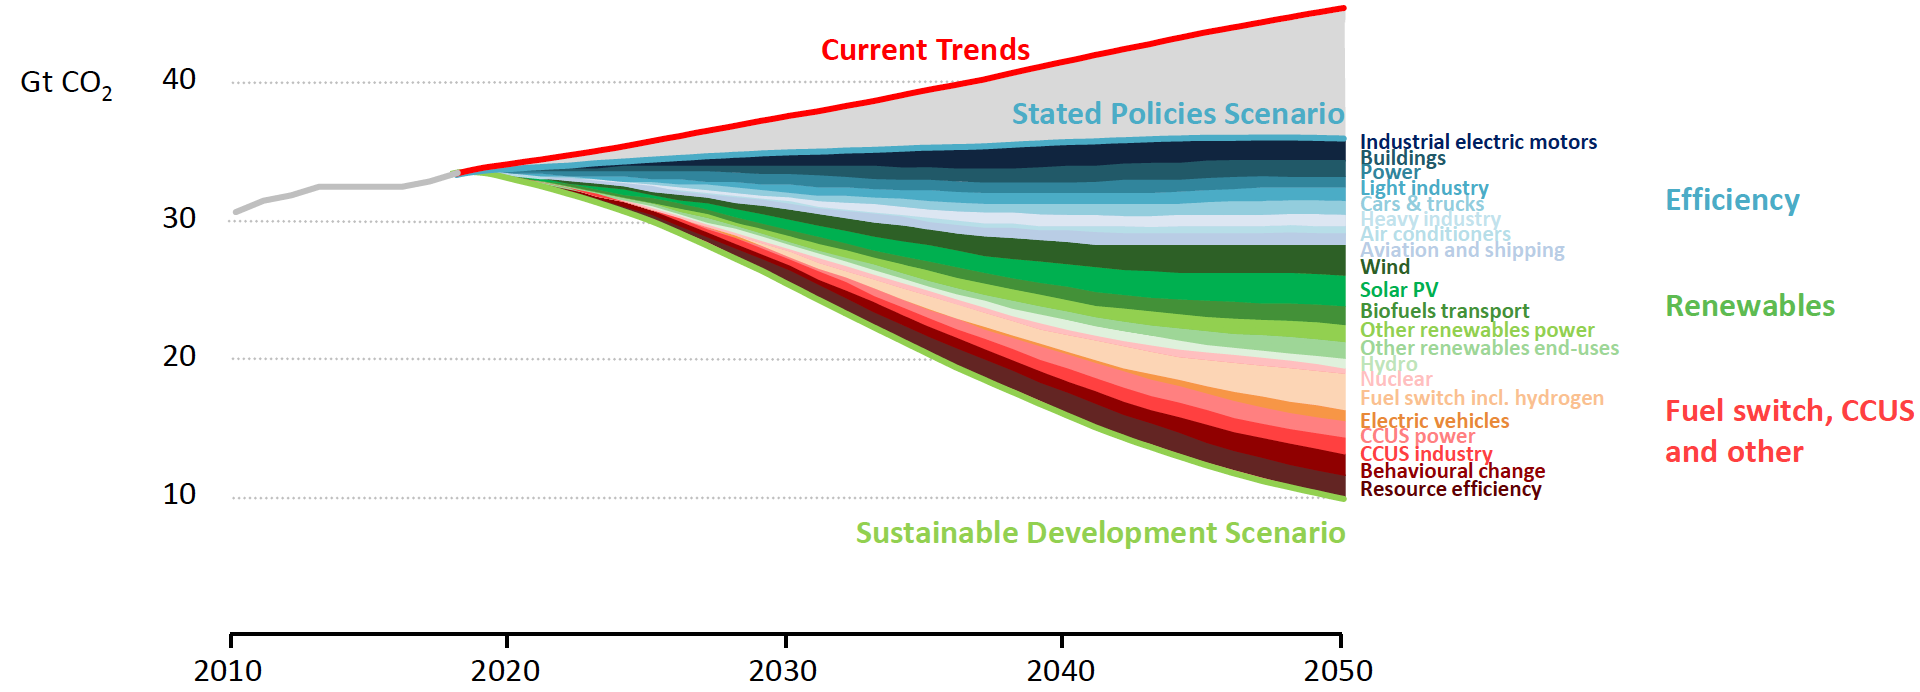
\includegraphics[width=\textwidth]{IEA_WEO_2019.png}
\caption{Energy-related CO2 emissions and reductions by sources in the Sustainable Development Scenario \cite{iea2020world}.}
\label{fig:intro:IEA_WEO_2019}
\end{figure}

In the general perspective to decrease the \gls{GWP} of the primary energy mix, \gls{VRES} like wind and solar, have already emerged as the keystone to defossilise the energy system. However, their intermittency and space disparity could hold back their vaster integration in the future. To address this issue, due to some limitations (\eg range, power, costs) of electricity-focused solutions like \gls{DC} lines, the transport and long-term storage of the renewable electricity produced in excess should be optimised. This challenge can be tackled by \textit{electrofuels} \cite{rozzi2020}. These fuels represent energy carriers where electricity has the major share in the energy balance of the fuel. In practice, this electricity is mainly converted into hydrogen (\ie electrolysis) and then potentially upgraded into more complex fuels (\eg methane, methanol or ammonia). Even if the share of electricity increases in the energy system through the electrification of the end-use demand, gaseous and liquid fuels will keep on being big players during (and after) the energy transition \cite{Ahlgren2012}. They offer three main advantages: infrastructure compatibility, storage and capacity to link sectors (\ie from electricity to mobility, heat, or industry). Development on electrofuels aims at getting them more and more compatible with existing and mature technologies \cite{Ahlgren2012}. An example is carbon-free ammonia-hydrogen blends burned in spark ignition engines \cite{lhuillier2020experimental} or \gls{CHP} applications \cite{pochet202022}. With a growing share of \gls{VRES}, sector coupling is essential to absorb the surplus of electricity from these intermittent production means \cite{robinius2017linking} and integrate them more cost-effectively \cite{brown2018response, limpensECOS2021}. Besides direct electrification of other sectors (\eg electrical heat pumps, \gls{BEV}), \citet{brown2018synergies} showed that converting power to hydrogen and methane was advantageous at high shares of renewables, in their optimisation of the European whole-energy system. Electrofuels have the ability to couple energy and non-energy sectors \cite{Stancin2020}. For instance, electricity produced in excess from \gls{VRES} can be converted into ammonia through the Haber-Bosch process and subsequently transformed into fertiliser - coupling the power and industry sectors \cite{verleysen2020can}. Gas networks present much more storage potential than electrical network (\eg 50 times more in Germany and 300 times more in France) \cite{Rosa2017}. Where batteries exhibit limited storage capacity (up to 10\,MWh) as well as self-discharge losses, electrofuels are an economical solution for high capacity (from 100 GWh) and long-term (\ie from months to years) storage of energy \cite{child2018role, dias2020energy} (see Figure \ref{fig:intro:Storage_electrofuels}). In their analysis of the German transport sector in 2050, \citet{millinger2021electrofuels} highlighted that producing electrofuels can represent a better usage of the ambient \ce{CO2} than \gls{CCS} to supply hydrocarbon fuels while limiting the curtailment of \gls{VRES}. Moreover, some applications (\eg marine, aviation and heavy-duty transport) will be hard to electrify and keep on requiring high-density energy carriers \cite{horvath2018techno, brynolf2018}. These carriers, currently produced from fossil resources, will still consist of hydrocarbons in a renewable world. This is why this thesis rather uses "defossilisation" rather than "decarbonisation" as carbon will still play a key role in a carbon-neutral energy transition \cite{mertens2020carbon}.

\begin{figure}[htbp!]
\centering
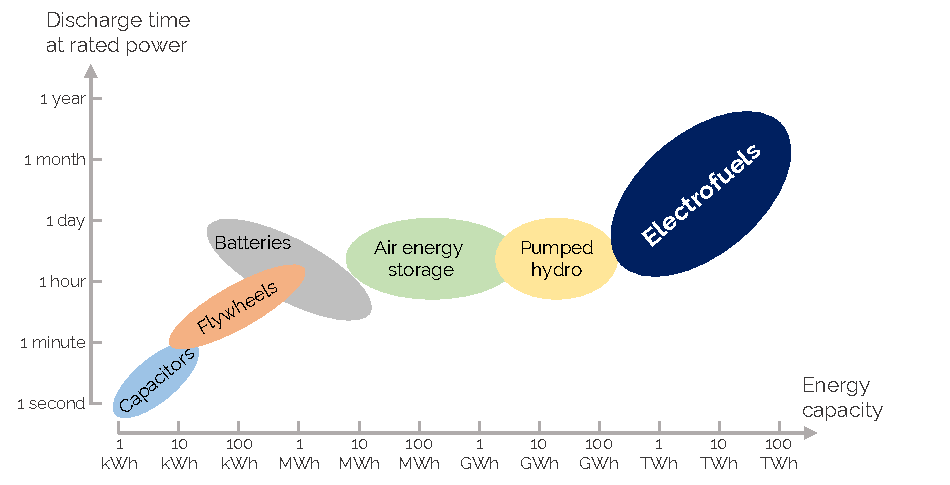
\includegraphics[width=0.9\textwidth]{Storage_electrofuels.pdf}
\caption{Energy carriers and technologies to store electricity. Electrofuels are an economical solution for high capacity and long-term storage of energy. Graph adapted from \cite{ISPT2017}.}
\label{fig:intro:Storage_electrofuels}
\end{figure}

To harvest the maximum potential of synthetic energy carriers in a sustainable transition and maximise the overall system efficiency \cite{mathiesen2015}, it is necessary to study the integration of these fuels within a multi-sector and whole-energy system \cite{Contino2020}. To reach this goal, an energy system optimisation model (ESOM) can optimise the design and the operation of the system to minimise, for instance, its costs or its emissions \cite{zeng2011review}. 

In this research field of energy system planning and scenario analysis, \citet{yue2018review} highlighted that most of ESOMs use a deterministic approach (\ie 75\% out of the 134 reviewed ESOM studies). However, the model structures are inherently uncertain as well as their numerous composing parameters, especially when it comes to define an energy transition strategy for a large-scale system, such as a country. Given the lifetime of the conversion technologies, such strategy implies decisions with long-term impacts (20 to 50 years) where forecasts can be highly unreliable \cite{Moret2017}. Besides the uncertainty on the model structure (not addressed in this work), this long-term and large-system optimisation motivates the need to account for \gls{UQ} and consider it as a major challenge of such models \cite{pfenninger2014energy}. This challenge, along with a large number (\ie more than a hundred) of uncertain parameters and limited information of their distribution, leads to the "curse of dimensionality" \cite{kuo2005lifting}, where the computational burden rapidly explodes with the number of considered uncertain parameters.

On top of dealing with these uncertainties, the reality of decision-makers is a limited foresight into the future \cite{poncelet2016myopic}. In a perfect foresight approach, decision-makers would be able to, from now on, see the ``finish-line of the transition'', \ie 2050 (and beyond), and make the planning decisions once and for all accordingly. On the contrary, they uncover the realisation of these uncertainties step-by-step (\ie in a ``myopic'' way), and progressively act on them to, hopefully, meet the set target to mitigate the climate change. In the objective to respect an overall \ce{CO2}-budget rather than to follow a prescribed \ce{CO2}-emissions trajectory, there was a need for a framework to explore these multiple transition pathways and provide insight about intermediate milestones not to miss. On top of the ``what to do?'', this approach aims at helping the policymakers to answer the  question ``how to do it?''.

Finally, when assessing the robustness of transition pathways provided by \gls{ESOMs}, the literature shows a variety of techniques, \eg Monte-Carlo analysis, stochastic programming or robust optimisation \cite{yue2018review}. However, the robustness is commonly applied to assess the sensibility of the solution regarding the objective function to optimise (\ie the total cost).  Given the complexity of whole-energy system models (\ie multiple sectors and multiple energy carriers) along with the time-scale of the transition and the lot of uncertainties, the total cost does not provide information on the sensibility of the design strategy, \ie the investment decisions. Where \citet{moret2020overcapacity} proposed a method to assess the robustness of a design by investigating the potential overcapacity needed to face uncertainties. However, their work focused on the power sector only and for a target future year, \ie 2035.  The literature was missing an approach to tackle these two challenges: to go beyond the total transition cost encompassing the details of a solution into a single value while assessing the whole-energy system over its whole transition.

\section*{Objectives and tasks}
``\textit{Our task is not to foresee the future, but to enable it.}'' Saint-Exupéry in Citadelle, 1948. In that sense, this thesis aims at providing decision-makers with new methods and informed policies accounting for the intrinsic uncertainties of the future.  Rather than trying, in vain, to answer the question ``What could possibly happen in the future?'', this work rather addresses the ``What could or should we do to make the future possible?''. Given these general context and motivations, the research questions are described as follows:
\begin{itemize}
\item What is the role of electrofuels in the transition pathway of a whole-energy system subject to uncertainties, limited foresight into the future and a \ce{CO2}-budget? What are the key uncertainties driving their import?
\item How to explore the multiple pathway possibilities through the optimisation of a policy, \ie sequence of actions to support a transition?
\item How to assess the robustness of a pathway roadmap defining the design strategy over the transition?
\end{itemize}

To answer these questions, several tasks have been carried out on the whole-energy system model accounting for the uncertainties, the method to explore the myopic pathway of such a system and the approach to assess the robustness of a pathway roadmap.  All this work has been applied to the case of Belgium, a densely populated country with a limited amount of renewable energies, which represents roughly one third of the forecast energy demand \cite{Limpens2020}. This makes it a challenging case to go from a highly fossil-dominated system in 2020 (\ie 73\% of the primary energy mix \cite{spf_economy_2022}) to carbon-neutrality by 2050. 

The model developed and used in the context of this thesis is EnergyScope Pathway \cite{limpens2024pathway}. First introduced by Limpens in his PhD thesis \cite{limpens2021generating}, this model optimises the design and the operation of a whole-energy system over several decades and accounts for the pathway transition from an existing system to a long term target, \ie 2050.  Compared to other models, EnergyScope Pathway introduces a rapid (\ie around 15~min on a personal laptop for the optimisation of a 30-year transition) computational optimisation tool for exploring diverse transition pathways within an entire energy system while maintaining temporal precision (\ie hourly time-resolution) to accurately capture the integration of \gls{VRES}. Based on this model originally implemented in a perfect foresight approach, \ie one overall optimisation for the whole pathway, we have developed the myopic method. In this, the whole time horizon (\ie 30 years) is optimised through a sequence of 10-year long time-windows having a 5-year overlap between each other. To address the question about the role of electrofuels, we have detailed further on their implementation in the model to account for four main ones: hydrogen, methane, ammonia and methanol. Moreover, given their current and (expected) future role into the sector of the \gls{NED}, we have implemented this sector with a similar level of detail as the other sectors of the system, \ie electricity, heat and transport. 

To account for uncertainties, we have used, and adapted to our case study, the work of \citet{Moret2017PhDThesis} and \citet{coppittersthesis} on the uncertainty characterisation and quantification, respecitvely. In his thesis, \citet{Moret2017PhDThesis} developed a framework to obtain uncertainty range for a variety of parameters like cost of purchasing and availability of resources or investment cost and efficiency of technologies. These ranges have then been sampled and propagated through the EnegyScope Pathway via the RHEIA framework developed by \citet{coppittersthesis}. Using the surrogate-modeling approach called \gls{PCE}, this framework allows identifying the uncertain parameters with the biggest impact on the variation of total transition cost or other outputs of interest like the imported amount of electrofuels. 

To explore the different pathway trajectories in this myopic optimisation process, we have applied the \gls{RL} method where an ``agent'' is trained through its interactions with its environment, EnergyScope Pathway, to optimise its policy, \ie sequence of actions to take to support the transition. Starting from the initial state of the energy system in 2020, the agent takes every five years a set of actions until reaching 2050. Although, these actions are taken every five years, they impact the system, for the next ten years - their time window. The intermediate solutions obtained in the middle of the time window are used as a new starting point for the agent that makes a new series of decisions for the next ten years, etc. Repeating the whole transition with different sequences of actions-states allow the agent to come up with an optimised policy towards sustainability, considering the variation of the parameters of its environment.

Finally, in the objective to assess the sensibility to uncertainties of different design transition roadmaps, we have defined an approach to come up with a ``robustness metric''. This approach is based on \gls{PCA} where directions capturing the widest design variations are identified and serve as a frame. Roadmaps resulting from perfect foresight optimisation have been tested in a myopic and uncertain pathways. The results of these myopic runs have then been ``projected'' on the aforementioned frame to be able to compare the robustness of different roadmaps between each other.

\section*{Outline}
This thesis is composed of five chapters to provide answers to the different research questions. Chapter \ref{chap:chap_methodo} brings more details about the different methodological aspects of this work. It starts with the main constraints, parameters and variables of the whole-energy system optimisation model, EnergyScope Pathway. Then, it gives information on the \gls{UQ} approach and the way it has been adapted to the case of Belgium and its transition pathway. Finally, general fundamentals and more case-specific considerations are brought up about the \gls{RL} and \gls{PCA}-based robustness approaches.

Chapter \ref{chap:case_study} presents the case study of this work, \ie Belgium and its energy transition. Without exhaustively detailing the data \cite{limpens2021generating}, this chapter focuses on the main contributions of this work regarding the case study: the \gls{NED}, the implementation of electrofuels and their respective routes of production and consumption, limiting  the cumulative emissions of the transition to a certain \ce{CO2}-budget rather than a prescribed emissions-trajectory and the date related \gls{SMR} as an option to produce nuclear-based electricity in the future.

Chapter \ref{chap:atom_mol} is the first of the three chapters presenting results. In this one, we detail the results of the \gls{GSA} carried out on the Belgian energy transition under the lens of the atom-molecules dilemma. On top of the impact of uncertainties on the total transition cost and the system design in general, we target the impact of having new nuclear capacities by 2040 onward and the driving parameters on the import of electrofuels.

In Chapter \ref{chap:chap_RL}, the rules of the ``\gls{RL} game'' are detailed. In other words, we define the action and state spaces as well as the reward function driving the behaviour of the agent in its quest to optimise its policy. Then, we analyse the results of the learning phase before testing under uncertainties the learned policy versus more ``classic'' myopic optimisation, \ie without the support of such a policy.

After detailing the robustness metric based on the \gls{PCA} approach, Chapter \ref{chap:chap_RobPol} assesses the robustness of different roadmaps resulting of deterministic perfect foresight optimisation under certain conditions: REF, SMR and ROB. The first one, the reference case, considers nominal values for all the uncertain parameters. The SMR case is the one introduced in Chapter \ref{chap:atom_mol} where we allow the model to install \gls{SMR} from 2040 onward. Eventually, the ROB case accounts for the highest values of parameters for those having the biggest impact on the total cost of transition (\ie cost of purchasing energy carriers, industrial \gls{EUD}, interest rate and variable \gls{OPEX} of technologies).

Finally, we draw general conclusions and suggest potential perspectives for future works in terms of uses and further developments of the methodological tools.
%\clearpage

%% -- Chapter 1 - Presentation of EnergyScope TD & Pathway + PCE + RL + PCA ---------------------------------
\chapter{Methodology: Through a variety of complementary tools}
\label{chap:chap_methodo}
\vspace{-0.2cm}
\begin{flushright}
\emph{``Technique aussi brûlante que les derniers bilans du GIEC.''}\\
 Primero (ft. Romeo), in \textit{Deux deux}, 2022
\end{flushright}
\vspace{0.4cm}
%\medskip
%
%\begin{mybox}{Chapter overview}
%\begin{itemize}[left=0em]%[leftmargin=0cm,itemindent=.5cm,labelwidth=\itemindent,labelsep=0cm,align=left]
%\setlength\itemsep{-0.3em}
%\item Belgian energy system overview%Case studies: the Belgian energy systems during the transition (2015-2050).
%\end{itemize}
%\vspace{-0.3cm}
%
%\emph{This chapter is an improved and extended case study version of \citet{Limpens_belgian_2020}}.
%\end{mybox}
%
%\medskip

Assessing the robustness of a whole-energy system transition pathway calls a variety of methodological tools. First and foremost, such an extensive system needs to be represented, \ie modelled, to further be optimised. This model requires some characteristics to capture the peculiarities of this system such as the intermittency of \gls{VRES}, the coupling between the different energy and non-energy sectors and a pathway vision to pave the way from where we are to where we want to go.  Then, as looking into the future (\ie up to 2050 in this work) comes with its lot of uncertainties, these have to be assessed carefully in terms of characterisation and quantification. The former aims at defining the range over which parameters of the model vary. The latter allows assessing the impact that such uncertainties can have on the output of the model. Finally, meeting the environmental objectives while minimising the cost of the system, accounting for this decision-making process, the uncertainties, and potential shocks/crisis, require therefore a framework to assess the relevance and the timing of the decisions throughout the transition. This work encompasses the optimisation of the policy, \ie set of actions to take along the transition with a specific methodology to assess its robustness. 

Detailing the different tools needed to answer the research questions, this chapter starts with the presentation of the whole-energy system optimization model, EnergyScope Pathway and its myopic formulation. Then, it focuses on the uncertainties, their characterisation as well as their quantification. Finally, an agent-based \acrfull{RL} approach is detailed to address the sequential decision-making process in the uncertain transition with limited vision in the future. The robustness of these policies is assessed via the use of the \gls{PCA}.

\section*{Contributions}
\label{sec:meth:contributions}
The main methodological contribution of this work is the implementation of the \gls{RL} approach to simulate and optimise the behaviour of an artificial agent interacting with its environment, \ie the the whole-energy system through its transition. Given the uncertainties and potential shocks of the future, this approach allows the agent to play the transition in a sequential, \ie myopic, way and optimise the choice and the timing of its actions. This optimization is done through trial and error where the agent repeats the transition with a new set of uncertainties. 

Then, to support this step-by-step transition with limited foresight in the future, we have extended the EnergyScope Pathway model \cite{limpens2021generating}. Originally developed to optimise the transition in one global optimisation up to 2050, \ie perfect foresight, part of this thesis consisted in making this model able to optimise the same transition but with sequential more limited time windows, \ie myopic approach. Besides its shorter computational time, this approach is more representative an actual decision process with limited foresight in the future \cite{babrowski2014reducing}.

The third principal methodological contribution is the use of \acrfull{PCA} to assess the robustness of a policy, \ie how much the optimal pathway is affected by the uncertainties. Given the uncertainties and the timespan of the transition, this approach allows highlighting the main \og directions'' of variation of the system design (\ie the installed capacities). After this step of identification, strategies and policies can be projected on these directions to see how robust they are to the overall transition uncertainties.

Finally, more minor methodological developments are part of this thesis. Following an approach similar to \citet{guevara2022modeling}, we have extended the ranges of uncertainty developed by \citet{Moret2017} to the pathway optimisation. After assessing the relevance of using \acrfull{PCE} on the optimisation of a whole-energy system \cite{limpens2020impact}, we have applied this uncertainty quantification method on the snapshot model subject to different emission-constraints \citet{rixhon2021role} as well as the pathway model. Eventually, starting from the initial investigation of \citet{goffauxpathway}, this work has converged to the most relevant formulation of the salvage value for the model EnergyScope. This aims at considering the residual value of assets that would still be in place after the end of the optimisation. It avoids penalising capital-intensive and long-lasting asset.In this formulation, the capacities that have been anticipatively decommissioned are removed from the total installed capacities. Therefore,  Therefore, this penalises decisions that would lead to investments that are later decommissioned before having reached the end of their lifetime.

\section*{Other authors' main contribution statement}
Novelty does not stand in the reinvention of the wheel.  This thesis, instead, finds its fundamentals in great tools previously developed by other authors. As developers of the building blocks of the main contributions of this thesis, three main authors are to be mentioned for having brought a significant part of the methodological work. Based on Stefano Moret's monthly whole-energy system model (\ie EnergyScope) \cite{moret2016strategic}, Gauthier Limpens has developed the hourly version of the snapshot model (\ie EnergyScope TD) \cite{limpens2019energyscope}, as well as the perfect foresight pathway model \cite{limpens2024pathway}, to which I personally contributed too. Diederik Coppitters has developed the RHEIA framework allowing to quantify the impact of uncertainties and carry out robust optimisation of energy systems \cite{coppittersthesis}. The current work used this framework for the first of these functionalities. Finally, Stefano Moret extensively assessed the uncertainty characterisation on the Swiss energy system \cite{Moret2017}. This thesis follows the same methodology, updating the uncertainty ranges for the pathway model.

\section[EnergyScope Pathway]{Whole-energy system transition model optimisation: EnergyScope Pathway}
\label{sec:meth:ES}

This work optimises the entire transition pathway from a known system in 2020 up to 2050 thanks to EnergyScope Pathway \cite{limpens2024pathway}. According to pathway models review (see Appendix \ref{app:ESPathway_choice}), EnergyScope Pathway can be categorised as an investment and operation optimisation model that assesses the whole-energy system, has a hourly time-resolution and is an open-source documented model. Moreover, it maintains a low computational cost (\ie around 15 minutes for a 30-year pathway with a hourly discretisation). From the perfect to the myopic foresight of the transition optimisation, this section presents only the main constraints of the former approach to further dig into more details about the latter. The reader is invited to refer to Appendix \ref{app:ESPathway_full_formulation} for more details about the formulation of the model and its extension from, EnergyScope TD, the a snapshot model, optimising a target future year with a greenfield approach \cite{geidl2006greenfield}. More extensive information about the formulation choices, for instance, can be found in \cite{limpens2024pathway} and the documentation \cite{readthedocs_pathway}.

\subsection{Perfect foresight: One global optimisation of the transition}
\label{subsec:meth:PF}

The whole-energy system model developed in this work originates from the perfect foresight (PF) formulation (\Cref{fig:meth_path_methodology_core}) of EnergyScope---the entire transition is computed in one optimisation, assuming a complete but uncertain knowledge of the different parameters until 2050 \cite{limpens2024pathway}. Each representative year is represented via the the variables and constraints of the snapshot model, EnergyScope TD \cite{limpens2019energyscope}. Then, to draw a consistent pathway between these years, additional constraints aim at linking them, \eg limiting the modal shifts within some energy sectors.

\begin{figure}[htbp!]
\centering
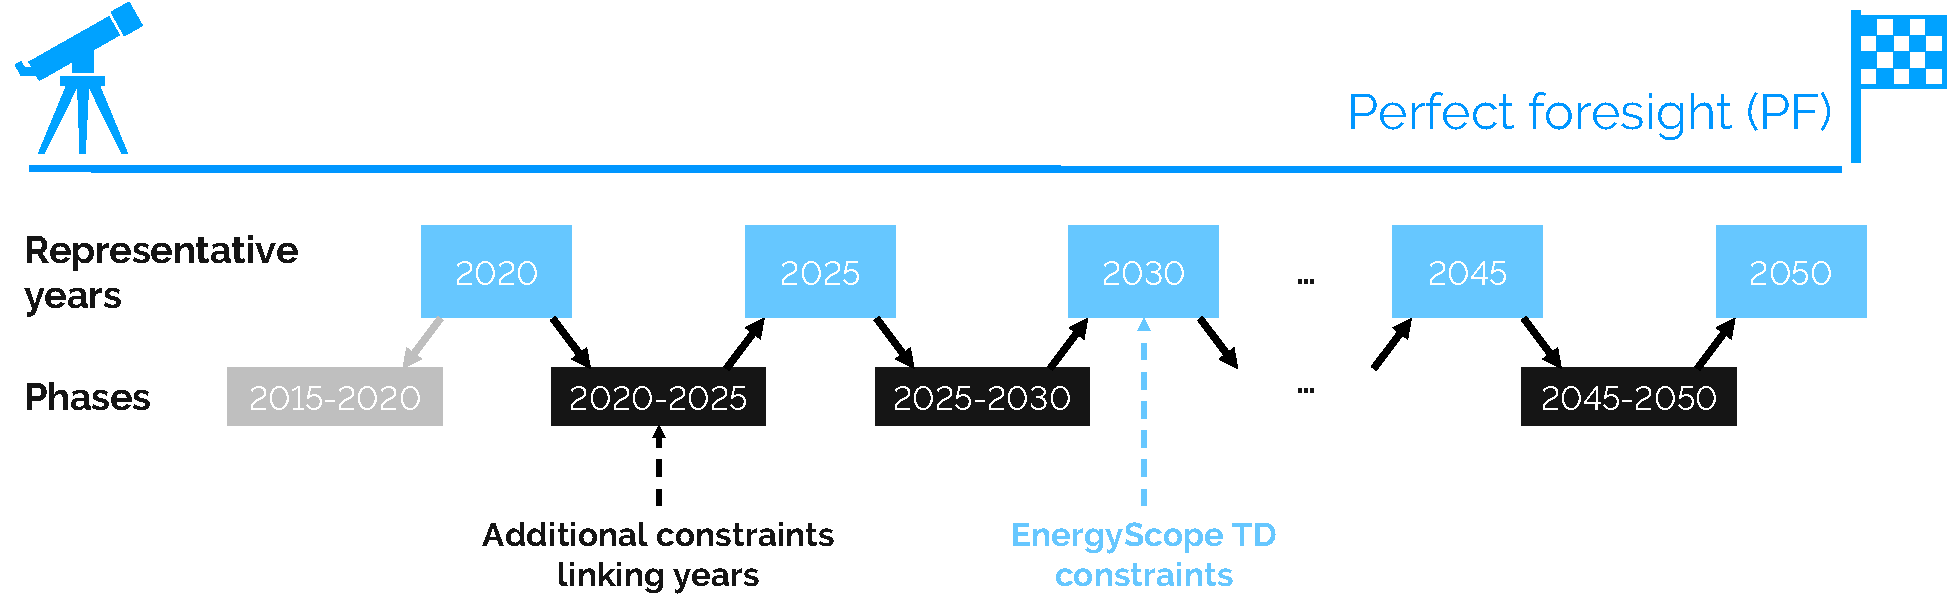
\includegraphics[width=\textwidth]{ES_Pathway.pdf}
\caption{Illustration of the pathway methodology based on an existing energy system model. The methodology spans from 2020 to 2050, with one representative year every five years. The model \acrfull{ESTD} is applied in 7 representative years (light blue boxes). The formulation includes additional constraints (black boxes) that link the years together. The pathway's initialisation assumes that all capacities installed in 2020 were built during the pseudo-phase of 2015-2020 (grey box). The overall problem is defined as the pathway model.}
\label{fig:meth_path_methodology_core}
\end{figure}

The objective function of the pathway model, \ie the total transition cost $\textbf{C\textsubscript{tot,trans}}$, is computed as the sum of the total \gls{CAPEX}, \textbf{C\textsubscript{tot,capex}}, and the \gls{OPEX}, \textbf{C\textsubscript{tot,opex}} (see Equation (\ref{eq:obj_func_v2})).

\begingroup
\vspace{-0.3cm}
\belowdisplayskip=2pt
\abovedisplayskip=2pt
\begin{flalign} 
% Objective function + investment 
\label{eq:obj_func_v2}%1
% adding 25pt space, otherwise flalign with two "&" would flush to the extreme 
\hspace{0pt} \min \text{  } & \textbf{C\textsubscript{tot,trans}} = \textbf{C\textsubscript{tot,capex}} + \textbf{C\textsubscript{tot,opex}}.&%\\
\end{flalign}
\endgroup

%\label{eq:Capex_v2_app}
%& \textbf{C\textsubscript{tot,capex}} =
%\sum_{\mathclap{p \in \text{\emph{PHASE}}\cup \{2015\_2020\}}} 
%\textbf{C\textsubscript{inv,phase}}(p)
%-
%\sum_{\mathclap{i \in \emph{TECH}}} 
%\textbf{C\textsubscript{inv,return}}(i)\\
%  \label{eq:Copex_tot_v2_app}%5
%& \textbf{C\textsubscript{tot,opex}} =  \textbf{C\textsubscript{opex}}(2020)
%+ \emph{t\textsubscript{phase}}\cdot \tau\textsubscript{\emph{phase}}(p) \cdot \sum_{\mathclap{p \in \emph{PHASE}|y\textsubscript{start}\in \emph{P\_START}(p),y\textsubscript{stop}\in \emph{P\_STOP}(p)}} 
% \Big(\textbf{C\textsubscript{opex}}(y\textsubscript{start}) + \textbf{C\textsubscript{opex}}(y\textsubscript{stop}) \Big)/2&\\
%\label{eq:path_annu_factor_app}
%& \tau\textsubscript{\emph{phase}}(p) = 1/(1+\emph{i\textsubscript{rate}})^{\emph{diff\_2015\_year(p)}} &
%% GL_correction_v2 %% & \tau\textsubscript{\emph{phase}}(p) = 1/(1+\emph{i\textsubscript{rate}})^{\emph{diff\_2015\_year(p)}} &

The total \gls{CAPEX} is the difference between the total investments done during the transition, $\textbf{C\textsubscript{inv,phase}}$, and the residual value of the assets that would still be in place after the end of the transition, $\textbf{C\textsubscript{inv,return}}$ (see Equation  (\ref{eq:CAPEX_v2})).

\begingroup
\begin{flalign} 
\belowdisplayskip=2pt
\abovedisplayskip=2pt
\label{eq:CAPEX_v2}
\hspace{0pt}&\textbf{C\textsubscript{tot,capex}} =
\sum_{\mathclap{p \in \text{\emph{PHASE}}\cup \{2015\_2020\}}} 
\textbf{C\textsubscript{inv,phase}}(p)
- \sum_{\mathclap{j \in \emph{TECH}}} \textbf{C\textsubscript{inv,return}}(j),&
\end{flalign}
\endgroup

\noindent
where $\textbf{C\textsubscript{inv,phase}}$ is given as the sum over all the  newly installed technologies at the phase $p$, $\textbf{F\textsubscript{new}}(p)$, multiplied by the average investment costs, $\emph{c\textsubscript{inv}}$,  of the year starting and ending the corresponding phase, $\emph{y\textsubscript{start}}$ and $\emph{y\textsubscript{stop}}$ respectively (see Equation (\ref{eq:PhaseInv})).

\begingroup
\belowdisplayskip=2pt
\abovedisplayskip=2pt
\begin{flalign} 
\hspace{0pt} 
\label{eq:PhaseInv}%5
&\textbf{C\textsubscript{inv,phase}}(p) = \sum_{\mathclap{j \in \emph{TECH}}} \textbf{F\textsubscript{new}}(p,j)\cdot \tau\textsubscript{\emph{phase}}(p)\cdot \emph{c\textsubscript{inv}}(p,j)&\forall p \in \emph{PHASE},
\end{flalign}
\endgroup

\noindent where $\tau\textsubscript{\emph{phase}}$ is the annualised phase factor and $\emph{c\textsubscript{inv}}(p,j)$ is the arithmetic average of the investment cost of the technology $j$ at the beginning and the end of the phase, $\emph{c\textsubscript{inv}}(\emph{y\textsubscript{start}},j)$ and $\emph{c\textsubscript{inv}}(\emph{y\textsubscript{stop}},j)$. The discount rate accounted for in the annualisation factor is considered as identical for all the technologies of the system. In practice, the discount rate would vary depending on the technology investment risk. Depending on the technology readiness level, private investors would be more or less risk-averse. However, EnergyScope only considers the vision of a central-planner where a single agent makes the investment decisions without differentiating the sources of the capitals, \ie private and public. Assuming a differentiated discount rate would require to make assumptions about the private-public distribution of the capitals. For this reason, we have decided to keep an identical value of discount rate for all the technologies.

Similarly, the salvage value is computed in the proportion of the remaining years of life versus the initial lifetime of an installed capacity of a technology from which the anticipatively decommissioned part, $\textbf{F\textsubscript{decom}}$, is removed (see Equation (\ref{eq:salvage}))

\begingroup
\belowdisplayskip=2pt
\abovedisplayskip=2pt
\begin{flalign} 
\label{eq:salvage}%5
&\textbf{C\textsubscript{inv,return}}(j) = \sum_{\mathclap{p \in \emph{PHASE}\cup \{2015\_2020\}}} 
\hspace{0.5cm}
 \tau_{phase}(p)\cdot \emph{c\textsubscript{inv}}(p,j) \cdot
&\notag\nonumber
\end{flalign}
\begin{flalign}
& 
\hspace{1.7cm}
\frac{remaining\_years(j,p)}{\emph{lifetime}(y\textsubscript{start},j)} \left( \textbf{F\textsubscript{new}}(p,j) - 
\sum_{\mathclap{p2 \in \emph{PHASE}}} 
\textbf{F\textsubscript{decom}}(p2,p,j)\right)&
\forall j \in \emph{TECH}.
\end{flalign}
\endgroup

About the total \gls{OPEX} of the transition, $\textbf{C\textsubscript{tot,opex}}$, on top of the initial costs in 2020, we assume that the \gls{OPEX} of a phase is equal to the average operational costs, $ \textbf{C\textsubscript{opex}}$,  of $\emph{y\textsubscript{start}}$ and $\emph{y\textsubscript{stop}}$, multiplied by the duration of a phase $\emph{t\textsubscript{phase}}$ equal to 5 years in our case (see Equation (\ref{eq:Copex_tot_v2})).

\begingroup
\begin{flalign} 
  \label{eq:Copex_tot_v2}%5
&\textbf{C\textsubscript{tot,opex}} =  \textbf{C\textsubscript{opex}}(2020)
+ \emph{t\textsubscript{phase}}\cdot \tau\textsubscript{\emph{phase}}(p) \cdot \sum_{\mathclap{p \in \emph{PHASE}}} 
\textbf{C\textsubscript{opex}}(p),&
\end{flalign}
\endgroup

\noindent
where $\textbf{C\textsubscript{opex}}(p)$ is the arithmetic average of the operational cost at the beginning and the end of the phase $p$,  $\textbf{C\textsubscript{opex}}(y\textsubscript{start})$ and $\textbf{C\textsubscript{opex}}(y\textsubscript{stop})$. The operational cost of a year, $y$, $\textbf{C\textsubscript{opex}} (y)$, is the sum of the costs related to maintenance and operation of technologies, $ \textbf{C\textsubscript{maint}}$, and the consumption of resources, $\textbf{C\textsubscript{op}}$ (see Equation (\ref{eq:opex_yearly})).


\begingroup
\belowdisplayskip=2pt
\abovedisplayskip=2pt
\begin{flalign} 
\hspace{0pt} 
\label{eq:opex_yearly}
&\textbf{C\textsubscript{opex}} (y) = \sum_{\mathclap{j \in \emph{TECH}}} \textbf{C\textsubscript{maint}}(y,j) + \sum_{\mathclap{i \in \emph{RES}}} \textbf{C\textsubscript{op}}(y,i) & \forall y \in \text{\emph{YEARS}},
\end{flalign}
\endgroup

\noindent
where the costs related to each representative year are:

\begingroup
\belowdisplayskip=2pt
\abovedisplayskip=2pt
\begin{flalign} 
% Objective function + investment 
% adding 25pt space, otherwise flalign with two "&" would flush to the extreme left
\hspace{0pt} 
 \label{eq:c_maint}%4
 &\textbf{C\textsubscript{maint}}(y,j) = c_{\text{\emph{maint}}}(y,j) \textbf{F}(y,j) & \forall y \in \text{\emph{YEARS}}, \forall j \in \text{\emph{TECH}}\\ 
  \label{eq:c_op}%5
 &\textbf{C\textsubscript{op}}(y,i) = \sum_{\mathclap{t \in T }} c_{\text{\emph{op}}}(y,i) \textbf{F\textsubscript{t}}(y,i,t) t_{op} (t)  
 & \forall y \in \text{\emph{YEARS}}, \forall i \in \text{\emph{RES}},
 \end{flalign}
 \endgroup

\noindent where the variable $\textbf{F}$ represents the size of the installed capacities (for all technologies $j$) and the variable $\textbf{F\textsubscript{t}}$ is the hourly consumption of the resources; the parameter $c_{\text{\emph{maint}}}$ is the OPEX of the technologies, and the parameter $c_{\text{\emph{op}}}$ is the cost of purchasing resources. For the sake of simplicity, as done by \citet{limpens2024pathway}, the sum over the 8760 hours of the year is written as the sum over $t \in T $. 

The \ce{CO2}-budget for the transition, $\textbf{GWP\textsubscript{tot,trans}}$ is equal to the arithmetic average of the representative years at the beginning and the end of each phase (see Equation (\ref{eq:gwp_tot_transition})). Similarly to initial operational costs to account for the system in place in 2020 (see Equation (\ref{eq:Copex_tot_v2})), $ \textbf{GWP\textsubscript{tot}}(2020)$ accounts for the entire operational emissions in 2020, as the initial cumulative emissions of the transition. Then, as detailed in Section \ref{sec:cs:CO2-budget}, these cumulative emissions is constrained by a budget (see Equation (\ref{eq:limit_gwp_trans})).

\begingroup
\belowdisplayskip=2pt
\abovedisplayskip=2pt
\begin{flalign} 
\label{eq:gwp_tot_transition}
&\textbf{GWP\textsubscript{tot,trans}}= \textbf{GWP\textsubscript{tot}}(2020) + \emph{t\textsubscript{phase}}\sum_{\mathclap{p \in \emph{PHASE}}}\textbf{GWP\textsubscript{tot}}(p) &
\\
\label{eq:limit_gwp_trans}
& \textbf{GWP\textsubscript{tot,trans}} \leq \emph{gwp\textsubscript{lim,trans}},&
\end{flalign}
\endgroup

\noindent
where $\textbf{GWP\textsubscript{tot}}(p)$ is the arithmetic average of the yearly emissions at the beginning and the end of the phase $p$,  $\textbf{GWP\textsubscript{tot}}(y\textsubscript{start})$ and $\textbf{GWP\textsubscript{tot}}(y\textsubscript{stop})$. The computation of these yearly emissions are based on the \acrfull{GWP} of the resources:

\begingroup
\belowdisplayskip=2pt
\abovedisplayskip=2pt
\begin{flalign}
\hspace{0pt}
 \label{eq:GWP_tot}%8
 & \textbf{GWP\textsubscript{tot}}(y)  =    \sum_{\mathclap{i \in \text{\emph{RES}}}} \textbf{GWP\textsubscript{op}}(y,i) 
 & \forall y \in \text{\emph{YEARS}}\\
  \label{eq:GWP_op}%7
 & \textbf{GWP\textsubscript{op}}(y,i) = \sum_{\mathclap{t \in T }} gwp_{\text{\emph{op}}}(y,i) \textbf{F\textsubscript{t}}(y,i,t)  t_{op} (t) & \forall y \in \text{\emph{YEARS}}, \forall i \in \text{\emph{RES}},
\end{flalign}
\endgroup

\noindent
where $gwp_{\text{\emph{op}}}$ is the specific emissions (\ie in kt$_{\ce{CO2},\text{eq}}$/GWh) of each resource. Based on an approach developed by the Intergovernmental Panel on Climate Change (IPCC) \cite{stocker2014climate}, this work considers the indicator ``GWP100a - IPCC2013'' to compute the emissions related to the use of resources. This includes the emissions due to the extraction, the transportation and the combustion of the energy carrier. EnergyScope proposes to account for the embodied emissions of the technologies based on a \gls{LCA}. These stand for extraction of materials, refining, construction and end of life \cite{schnidrig2023integration} and can be one to three times higher than the direct emissions depending on the level of emission reduction \cite{blanco2020life}. However, this work is still in progress and the database is not yet complete. Consequently, it is not included in this work and not accounted for. 

Besides this constraint on the emissions, the main constraint to link years with each other is the one dictating the installed capacities at the end of each year:

\begingroup
\belowdisplayskip=2pt
\abovedisplayskip=2pt
\begin{flalign} 
\label{eq:F_newBuilt}%5
&\textbf{F}(y\textsubscript{stop},j) = \textbf{F}(y\textsubscript{start},j)
 + \textbf{F\textsubscript{new}}(p,j)
 - \textbf{F\textsubscript{old}}(p,j)
 - \sum_{\mathclap{p2 \in \text{\emph{PHASE}} \cup \{2015\_2020\}}} \textbf{F\textsubscript{decom}}(p,p2,j)& \notag \nonumber 
 \end{flalign}
\begin{flalign} 
 &&  \forall p \in \text{\emph{PHASE}}, \emph{y\textsubscript{stop}} \in \emph{Y\_STOP}(p), \emph{y\textsubscript{start}} \in \emph{Y\_START}(p), j \in \text{\emph{TECH}},
 \end{flalign}
\endgroup

\noindent
where the variables $\textbf{F\textsubscript{old}}$ and $\textbf{F\textsubscript{decom}}$ are the capacities respectively having reached the end of their lifetime and prematurely decommissioned. Moreover, to account for the society inertia and to prevent unrealistically fast modal share change, constraints limit this change for the sectors of the low-temperature, the passenger mobility and freight mobility demands. The interested reader will find more information about the formulation choices related to it in the work of \citet{limpens2024pathway}. 

\subsection[Myopic: Sequential optimisation of the transition]{Myopic: Sequential optimisation of the transition with limited foresight}
\label{subsec:meth:MY}

One of the main methodological contributions of this work regarding the development of the whole-energy system model consists in giving it the possibility to optimise the transition pathway in a myopic approach. After introducing the general concept, this section details more the additions brought to the model in terms of implementation.\\

\myparagraph{General concept of the myopic optimisation}\\

Compared to the perfect foresight, the myopic approach (Figure \ref{fig:my_schematic}) has three main advantages: shorter computational time, more realistic representation of the short-sightedness of decision-makers and the ability to capture shocks and unexpected events \cite{mccollum2020energy}. For this reason, several studies are based on this approach \citep{babrowski2014reducing,poncelet2016myopic,nerini2017myopic,heuberger2018impact}. \citet{babrowski2014reducing} analysed the benefit of the myopic approach to reduce the computational time. \citet{poncelet2016myopic} uses this approach to analyse the expansion planning of the power sector beyond 2050 to assess the realism of the decision making process brought up by the myopic implementation. \citet{nerini2017myopic} analysed the impact of the horizon windows and overlapping time.  Overall these studies decided to choose the myopic approach to analyse the speed of change compared to a perfect foresight approach.
 % rajout du Réalisme 
Moreover, the myopic approach allows a sequential optimisation process that opens the doors to decision-making/policy-learning methodologies, like assessing shock events. This approach is used by \citet{heuberger2018impact} who assessed the speed of integration of technologies due to these events. 
In their analysis of the overcapacity in European power systems, \citet{moret2020overcapacity} emphasised that such a ``possibility of \textit{recourse}" is very appropriate to address uncertainty gradually unfolding over time. Consequently, the development of the myopic approach with an overlap between two successive time windows has been implemented. This sequential optimisation framework also represents the foundations of the further implementation of the agent-based reinforcement learning framework (see Section \ref{sec:meth:RL}).

\begin{figure}[htbp!]
\centering
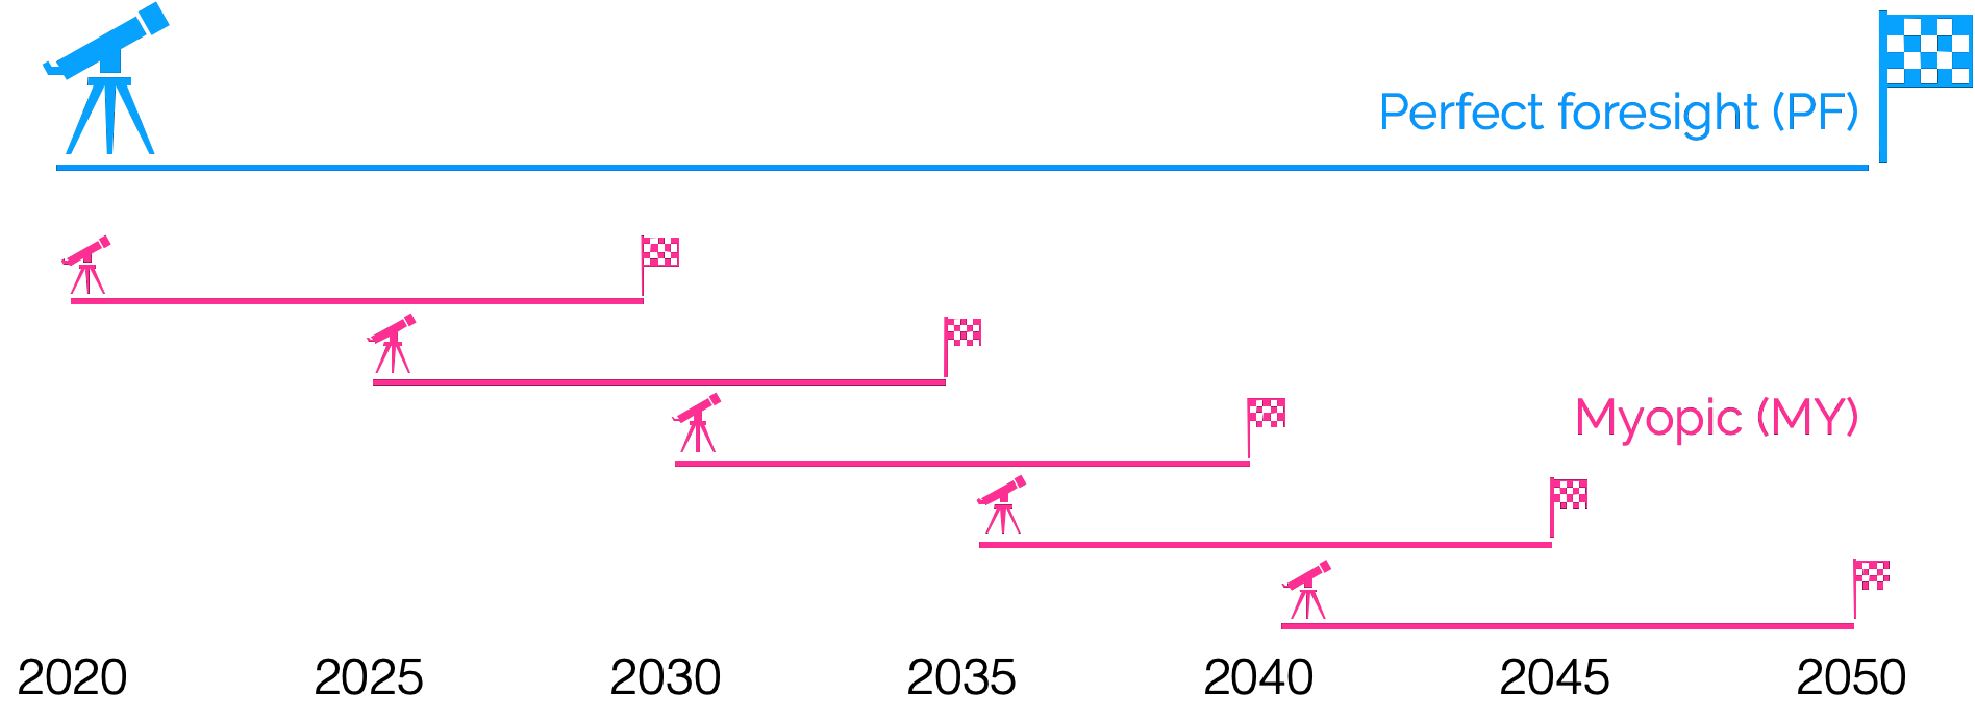
\includegraphics[width=\textwidth]{MY_schematic.pdf}
\caption{The myopic approach (in pink) uses several instances of the pathway model (illustrated in Figure \ref{fig:meth_path_methodology}). In this example, the pathway instance has a time horizon of 10 years ($N\textsubscript{year,opti}=10$) with a 5 year-overlap ($N\textsubscript{year,overlap}=5$). As a comparison the Perfect foresight (in blue) has a time horizon of 30 years.}
\label{fig:my_schematic}
\end{figure}

After optimising, in design and operation, one time window (\eg from 2020 to 2030), the intermediate system design (\ie the installed capacities) is set as initial conditions for the start of the next time window (\eg from 2025 to 2035) as well as the historical investment decisions (\ie $\textbf{F\textsubscript{new}}$, $\textbf{F\textsubscript{old}}$ and $\textbf{F\textsubscript{decom}}$) (see Figure \ref{fig:my_schematic_2}). Consequently, the solution obtained at the end of the first time window (\eg 2030) as well as potential investment decisions between the start of the second time window and this end-year are discarded. In other words, they are not taken into account for the optimisation of the second time window since the new final year is further into the future. This process goes on until the stated end of the transition (\ie 2050, in this case).

\begin{figure}[htbp!]
\centering
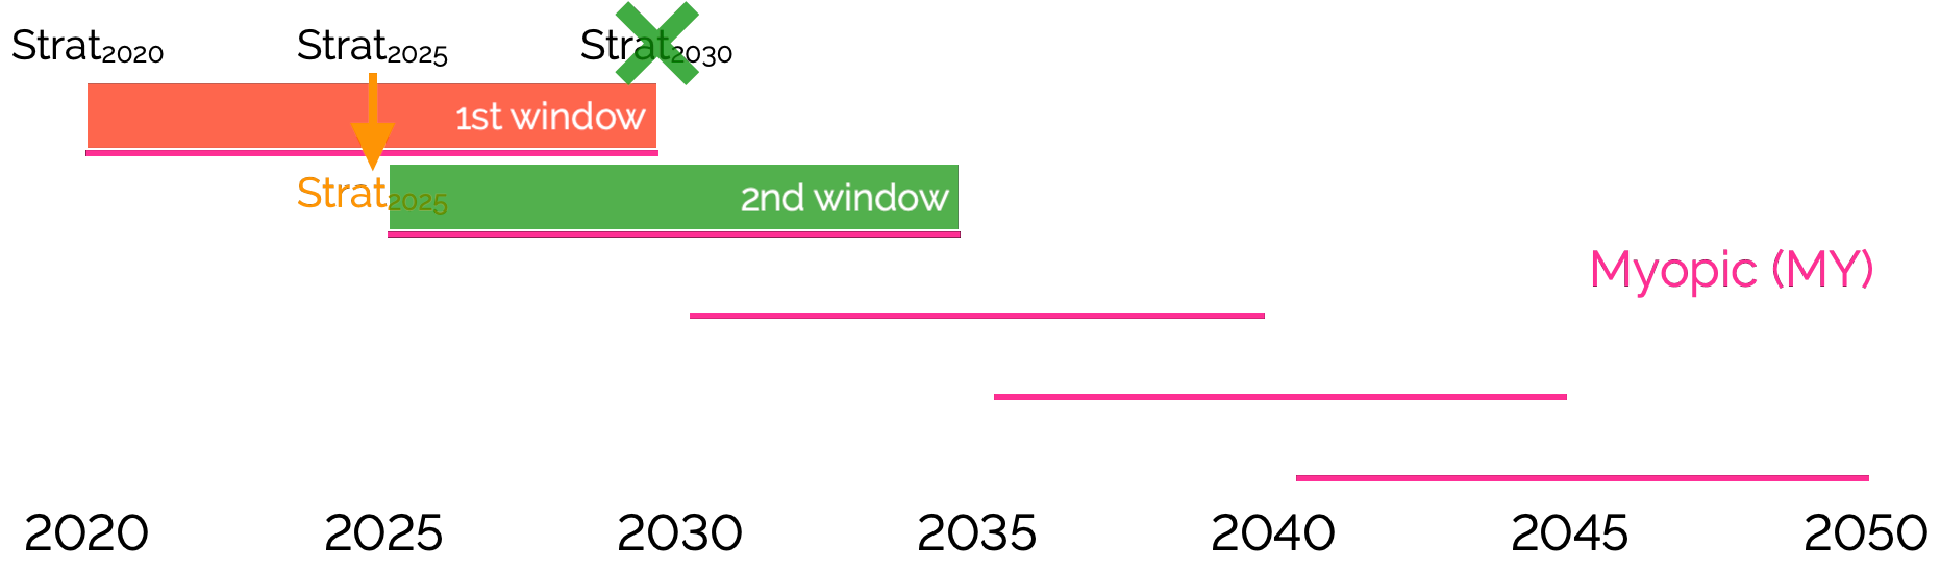
\includegraphics[width=\textwidth]{MY_schematic_2.pdf}
\caption{Sequential optimisation of the transition pathway in the myopic approach: (i) first time-window optimisation, (ii) set-up of the initial conditions of the second time-window, (iii) second time-window optimisation discarding intermediate results}
\label{fig:my_schematic_2}
\end{figure}

\myparagraph{Additional sets, parameters and variables}\\

\noindent
The major add-on from the original EnergyScope Pathway model \cite{limpens2021generating} to the myopic version developed in this thesis, is the possibility to carry out the optimisation on a limited time window, of which the duration is defined by $N\textsubscript{year,opti}$. Moreover, there is also the possibility of having an overlap between two consecutive time windows. The timespan of this overlap is defined by the parameter $N\textsubscript{year,overlap}$. The philosophy followed behind the development of the myopic approach was to add another layer on top of the perfect foresight model in order to make it more modular. For this reason, the already existing constraints are marginally adapted. This way, the newly developed model can easily be used to perform a perfect foresight optimisation by setting the time window to $N\textsubscript{year,opti}=$30 years (\ie between 2020 and 2050) and the overlap between the time windows to $N\textsubscript{year,overlap}=$0.  Consequently, as it is fundamental to define, on the one hand, the actual time window on which the system is optimised, and on the other hand, the history, \ie what has already been optimised earlier in the transition, four new sets are implemented: $\text{YEARS}\textsubscript{WND}$, $\text{YEARS}\textsubscript{UP TO}$, $\text{PHASE}\textsubscript{WND}$ and $\text{PHASE}\textsubscript{UP TO}$ (see Table \ref{tab:path_my_sets}).

\begin{table}[htbp]
\caption[New SETs for myopic pathway formulation.]{New SETs for myopic pathway formulation.} 
\label{tab:path_my_sets}
%\begin{minipage}{\textwidth}
\centering
%\resizebox{\textwidth}{!}{
\begin{tabular}{l c l}
\toprule
\textbf{Set}      & \textbf{Index}	 &	\textbf{Description}\\
\midrule
$\text{YEARS}\textsubscript{WND}$ 	&	$y\in$Y	& 	\pbox{20cm}{\vspace{1mm} Representative years of the \\ time window to optimise}\\
$\text{YEARS}\textsubscript{UP TO}$ &	$y\in$Y	& 	\pbox{20cm}{\vspace{1mm} Representative years including the \\ years already optimised, \ie the history}\\
$\text{PHASE}\textsubscript{WND}$ &  $\emph{p}\in$P & 	\pbox{20cm}{\vspace{1mm} Phases of the time window to optimise}\\
$\text{PHASE}\textsubscript{UP TO}$ &  $\emph{p}\in$P & 	\pbox{20cm}{\vspace{1mm} Phases including the phases \\ already optimised, \ie the history}\\
\bottomrule
\end{tabular}%}
%\end{minipage}
\end{table}

$\text{YEARS}\textsubscript{WND}$ and $\text{PHASE}\textsubscript{WND}$ substitute $\text{YEARS}$ and $\text{PHASE}$ in the constraints defined in the pathway model in Section \ref{subsec:meth:PF}. These two sets aim at setting the optimization to a more limited time window. Progressing through the transition, $\text{YEARS}\textsubscript{UP TO}$ and $\text{PHASE}\textsubscript{UP TO}$ allow keeping track of the history of the investments (\eg technologies installation, decommissioning or retirement), the consumption of resources, the cumulative amount of emissions, etc.

On top of these four specific sets, some artefacts were also necessary to avoid computational rounding errors. For instance, the first year of a time window is the result of the optimisation of the previous one. Therefore, optimising again this first year could lead to rounding errors preventing from the optimization to converge. For this reason,  the set $\text{YEAR}\textsubscript{ONE}$ accounts for the first representative year of the time window to optimise that is excluded from $\text{YEARS}\textsubscript{WND}$ to avoid these errors. This remark stays valid for any time window except the first one of the transition where the year 2020 is optimised even though its technological strategy is set according to the actual system presented in Appendix \ref{app:bel_2020}. Finally, as the end of time windows changes for each of them, the parameter $remaining\_years$ has to be updated accordingly to keep a meaningful definition of $\textbf{C\textsubscript{inv,return}}$ in Equation (\ref{eq:salvage}).\\

\myparagraph{Myopic pathway implementation}\\

\noindent
Starting this work in 2017, AMPL Optimization Inc. has developed a Python \gls{API} called amplpy \cite{amplpy}. In a nutshell, this API allows the pre/post-processing of an ampl optimisation problem by accessing its features (\eg constraints,parameters, variables, objective function) from within Python. Using this \gls{API}, this updated version of the model interacts with the AMPL problem representing the optimisation of the whole-energy system transition pathway as represented in Figure \ref{fig:MY_process_code}. \\


\begin{figure}[htbp!]
\centering
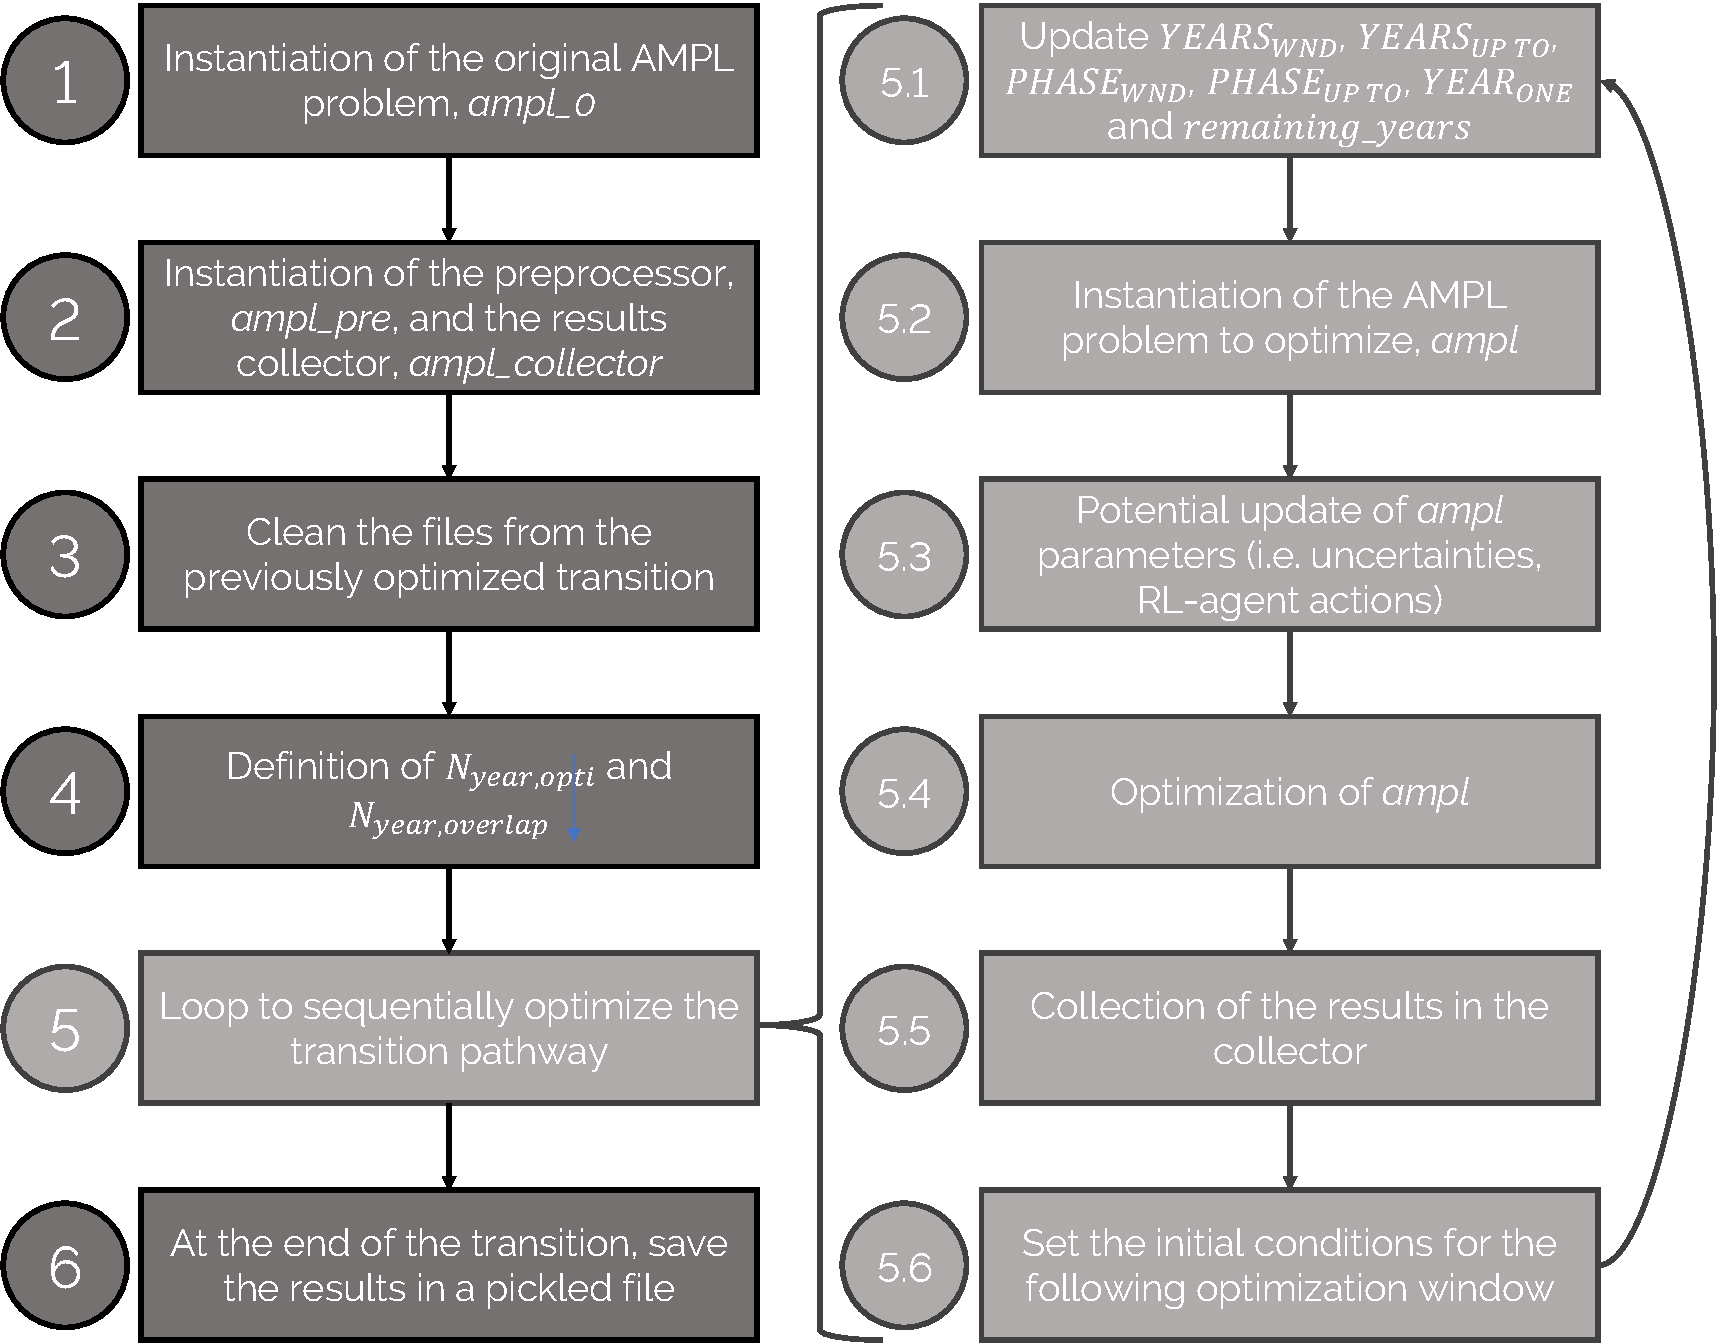
\includegraphics[width=10cm]{MY_process_code.pdf}
\caption{Schematic of the iterative optimisation of the whole-energy system transition pathway.}
\label{fig:MY_process_code}
\end{figure}

\myparagraph{Impact of myopic formulation on the system}\\

\noindent
In line with the work of \citet{babrowski2014reducing}, the computational time is reduced drastically (\ie by 55\%). On top of this, we observed that the resulting design, \ie the technological mix, remains similar.  Given the continuous change of the input parameters over the considered time frame, the perfect foresight and myopic approaches results are very similar, like in \cite{krey2006vergleich}: less than 1\% cost difference over the transition, similar system designs by 2050 and slight shifts in time in terms of adoption of technologies. 

The main difference lies in the myopic transition itself and especially in the earlier deployment of PVs and offshore wind turbines. These induce the reinforcement of the grid that is a capital-intensive and long-lifetime asset. This is mostly due to impact of the salvage value, Equation (\ref{eq:salvage}), in the objective function. Since this is now the transition cost over a more limited time window (\ie 10 years rather than 30 years), a bigger salvage value, deduced from the total investments, leads to a temporary better optimum at early stages of the transition. A more detailed comparison between the myopic and perfect foresight approaches is available in Appendix \ref{app:my_vs_pf}.

\section{Uncertainty quantification}
\label{sec:meth:UQ}
In their systematic review, \citet{yue2018review} highlighted that a wide majority of studies addressing the optimisation of energy systems (\ie 75\% out of the 134 reviewed studies) were not investigating the impact of uncertainties. However, disregarding these impacts can have drastic consequences on the system design. For instance, historical low \gls{NG} prices have led to overcapacity of \gls{CCGT} in Europe \cite{moret2020overcapacity}. This is why accounting for uncertainty in \gls{ESOMs} is crucial \cite{mavromatidis2018uncertainty}, especially when it comes to optimise several decades in an inherently uncertain future \cite{peace2008insights}.

This section aims at briefly presenting the methods followed to first characterise these uncertainties, then to quantify their impact on different outputs of interest of the model (\eg amount of molecules imported from abroad, the installed capacity of \gls{SMR} or the total transition cost) and finally, the screening and selection of the parameters to analyse.

\subsection{Uncertainty characterisation}
\label{subsec:uncert_charac}
Characterising precisely the uncertainty---ideally with their respective probability density functions (PDFs)---of the thousands of parameters in the model is daunting if not impossible because of lack of data \cite{marnay2006addressing}. Therefore, we used a workaround developed by \citet{Moret2017} that defines relative ranges of variation for different groups of parameters. These ranges have been adapted for the Belgian energy system and the pathway formulation. Moreover, some ranges have been added to account for new parameters coming from the pathway formulation described in Section \ref{sec:meth:ES} like the society inertia. Like other works \cite{li2019renewables,coppitters2021robust} and given the scarcity of information, the uncertain parameters are assumed to be independent and uniformly distributed between their respective lower and upper bounds. Alternatives like PERT or Gaussian distributions could also have been considered \cite{coppittersthesis}.

%\Cref{tab:UC_short} gives the uncertainty ranges of some key parameters. A particular attention is to pay to the potential installation of \gls{SMR}, at the bottom of \Cref{tab:UC_short}. As detailed in \Cref{sec:cs:technologies}, the commercial availability of such a technology is uncertain but would not be before 2040. Consequently, for \gls{SMR}, the parameter $f_{\mathrm{max,SMR}}$ influences the maximum capacity to install to translate somehow the readiness of this technology. As SMRs are foreseen, if installed, to be around the same locations (\ie Tihange and Doel) as the conventional nuclear power plants and using the same area in kW/ha, the same 6\,GW are assumed to be the maximum capacity for SMRs. If it is (i) smaller than 0.6, there is no possibility to install \gls{SMR} during the transition; (ii) between 0.6 and 0.8, these 6~GW can be installed only in 2050; (iii) between 0.8 and 0.9, these can be installed from 2045 onward and; (iv) higher than 0.9, the prescribed maximum capacity can be installed from 2040 onward. Based on the local sensitivity analysis carried out by \citet{PATHS2050}, the current work also considers a [-40\%; +44\%] range on the CAPEX of SMR, on top of the uncertainty about the availability. Finally, the the cost of purchasing renewable electrofuels presents a wide range, [-64.3\%; +179.8\%], like the other imported commodities.

%The exhaustive list of the parameters accounted in this work is presented in Appendix \ref{app:UC_full}.

%\begin{table}[htbp!]
%\caption{Illustration of the uncertainty characterisation for different parameters for the year 2025. $^{(a)}$ Per \cite{Moret2017PhDThesis}, \og I: investment-type, II: operation-type (constant uncertainty over time), III: operation-type (uncertainty increasing over time)\fg. $^{(b)}$ The nominal value of each parameter is 0, meaning no variation compared to the nominal values of the impacted parameter in the model. $^{(c)}$ This range has been inferred from the local sensitivity analysis performed by \citet{PATHS2050}.}
%\label{tab:UC_short}
%\centering
%\resizebox{\textwidth}{!}{
%\begin{tabular}{l l l c c c}
%\toprule
%\multirow{2}{*}{\textbf{Category}} & \multirow{2}{*}{\textbf{Parameter}} & \multirow{2}{*}{\textbf{Meaning}} & \multirow{2}{*}{\textbf{Type}$^{(a)}$}  & \multicolumn{2}{c}{\textbf{Relative variation$^{(b)}$}}\\
%    & & & &	 min 	&	 max \\ 	
%\midrule		
%\multirow{2}{*}{\textbf{Cost of purchasing}} & $c_{\mathrm{op,fossil}}$ & Purchase fossil fuels & II & -64.3\% & 179.8\% \\
%& $c_{\mathrm{op,electrofuels}}$ & Purchase electrofuels & II & -64.3\% & 179.8\% \\
%\midrule
%\multirow{5}{*}{\textbf{Investment cost}} &$c_{\mathrm{inv,car}}$ & CAPEX car  & I & -21.6\% & 25.0\% \\
%& $c_{\mathrm{inv,e\_prop}}$ & CAPEX electric motor & I & -39.6\% & 39.6\% \\
%& $c_{\mathrm{inv,fc\_prop}}$ & CAPEX fuel cell engine & I & -39.6\% & 39.6\% \\
%& $c_{\mathrm{inv,PV}}$ & CAPEX PV & I & -39.6\% & 39.6\% \\
%& $c_{\mathrm{inv,nuclear\_SMR}}$ & CAPEX \gls{SMR}$^{(c)}$ & I & -40.0\% & 44.0\% \\
%\midrule
%\multirow{1}{*}{\textbf{Consumption}} &$\eta_{\mathrm{e\_prop}}$ & Consumption electric vehicles & I & -28.7\% & 28.7\% \\
%\midrule
%\multirow{2}{*}{\textbf{Potential installed capacity}} &$f_{\mathrm{max,PV}}$ & Max capacity PV & I & -24.1\% & 24.1\% \\
%& $f_{\mathrm{max,windon}}$ & Max capacity onshore wind & I & -24.1\% & 24.1\% \\
%\midrule
%\multirow{2}{*}{\textbf{Hourly load factor}} & $c_{\mathrm{p,t,PV}}$ & Hourly load factor PV & II & -22.1\% & 22.1\% \\
%& $c_{\mathrm{p,t,winds}}$ & Hourly load factor wind turbines & II & -22.1\% & 22.1\% \\
%\midrule
%\multirow{2}{*}{\textbf{Resource availability}} & $avail_{\mathrm{elec}}$ & Available electricity import & I & -32.1\% & 32.1\% \\
%& $avail_{\mathrm{biomass}}$ & Available local biomass & I & -32.1\% & 32.1\% \\
%\midrule
%
%\multirow{2}{*}{\textbf{End-use demand}} & $pass\_EUD$ & Passenger mobility EUD & III & -7.5\% & 7.5\% \\
%& $industry\_EUD$ & Industry EUD & III & -20.5\% & 16.0\% \\
%\midrule
%
%\multirow{4}{*}{\textbf{Miscellaneous}} &$i_{\mathrm{rate}}$  & Discount rate & I & -46.2\% & 46.2\% \\
%& $\Delta_{\mathrm{change,freight}}$ & Modal share change freight mobility & - & -30\% & 30\% \\
%& $\Delta_{\mathrm{change,pass}}$ & Modal share change passenger mobility & - & -30\% & 30\% \\
%& $f_{\mathrm{max,SMR}}$ & Potential capacity \gls{SMR} & - & 0 & 1 \\
%
%\bottomrule							
%
%\end{tabular}}
%\end{table}

Following the methodology defined by \citet{Moret2017}, uncertainties of types I (investment-type) and II (operation-type, constant uncertainty over time) keep the same range width for the whole transition. In other words, unlike type III parameters, this width is not expanding (nor narrowing) for the different representative years of the transition. However, parameters with an uncertainty increasing over time, type III, (\ie end-use demands, in this case) will have a wider and wider range over the transition (see Figure \ref{fig:ranges_transition}). In this work, a +50\% linear increase has been set between the width of the range of such parameters in 2025 and the same ranges in 2050. This choice leads to an industrial \gls{EUD} that could be, in 2050, -30.8\% compared to its nominal value. This potential drop compared to the reference is in line with the work of \citet{My2050}. In their work, the total energy demand in the industry sector in 2050 could be between -19\% to -50\% of the reference value, depending on the scenario. In \Cref{fig:ranges_transition}, this means that for type III uncertainties only, $R_{2050}^+$ is 50\% bigger than $R_{2025}^+$ and $R_{2050}^-$ is 50\% smaller than $R_{2025}^-$. For uncertainties of types I and II, the relative variation versus the nominal value remain the same over the transition. Inspired by \citet{guevara2022modeling}, the values of the uncertain parameters are set at a fixed relative position from the nominal values for each sampled transition---the values do not zigzag from 2025 to 2050 within the bounds (\Cref{fig:ranges_transition}).

\begin{figure}[htbp!]
\centering
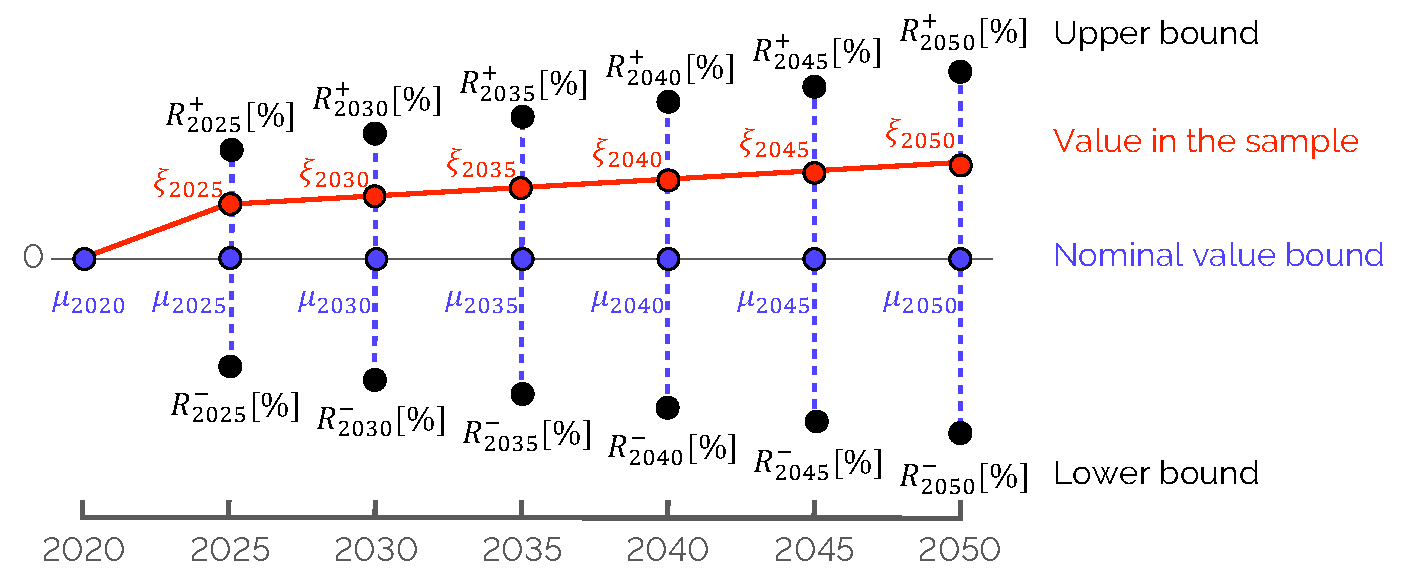
\includegraphics[width=0.7\textwidth]{ranges_transition.pdf}
\caption{Expansion of the width of uncertainty range for type III parameters. $\mu_{2020}$, $\mu_{2025}$, ...,  $\mu_{2050}$ are the nominal values equal to 0 as the uncertain parameters represent a relative increase/decrease of actual parameters of the model. $R^+$ and $R^-$ are respectively the upper and lower bounds of the range and $\xi_{2025}$, $\xi_{2030}$, ...,  $\xi_{2050}$ are the values taken by one parameter for a specific sample of the \gls{GSA} for each of the representative years of the transition, always starting from the nominal value in 2020, $\mu_{2020}$. The graph has been adapted from \cite{guevara2022modeling}.}
\label{fig:ranges_transition}
\end{figure}

\newpage
Finally, the model accounts for thousands of parameters. The computational burden to consider all of them separately would be completely overwhelming ($\sim 10^7$ model runs\footnote{As detailed in Section \ref{subsec:pce}, the number of runs required for the \gls{GSA} is proportional to the factorial of the number of uncertain parameters. As second order \gls{PCE} is the minimum to ensure accuracy of the surrogate model, considering thousands of independent uncertain parameters would lead to millions of runs, if no more.}). Similarly to other works \cite{Moret2017,limpens2020impact}, the model parameters that would follow the same uncertainty have been grouped to one single uncertain parameter. On top of mitigating the computational burden, this aims at grouping parameters that are closely linked with each other. For instance, the uncertainty on the cost of purchasing renewable electrofuels, $c_{\mathrm{op,electrofuels}}$, identically affects the cost of e-hydrogen, e-methane, e-ammonia and e-methanol. Indeed, besides their respective specificities, each of these fuels will be similarly affected by the variation of cost of electricity or the electrolyser, that drive the majority of their cost of purchasing \cite{h2coalition}. Similarly, the uncertainties impacting the industrial demand, $industry\_\emph{EUD}$, alters equally the industrial high- and low-temperature and electricity demands as well as the non-energy demand.

\subsection{Polynomial Chaos Expansion}
\label{subsec:pce}

To avoid the avoid the computational burden of well-known method like Monte-Carlo analysis \cite{yue2018review}, we used \gls{PCE} to carry out a \gls{GSA}. \gls{PCE} is an approach for surrogate-assisted \gls{UQ} that propagates uncertainties in input parameters through the system model. This allowed us to assess statistical moments on the quantity of interest and determine Sobol' indices~\cite{coppitters2020robust}. To construct a PCE of the EnergyScope Pathway model, we employed the open-source Python framework RHEIA~\cite{coppitters2022rheia,readthedocs_rheia}. Where the first part of this section is dedicated to the mathematical definition of this approach, the second details its choice and summarises the comparison made with another approach (\ie Morris method) in a previous work \cite{limpens2020impact}.\\

\myparagraph{Definition}\\

\noindent
The PCE model ($\hat{M}$) is a representation of the relationship between the input parameters and the output variable of interest (\ie the value of the objective function, see Equation (\ref{eq:obj_func_v2})) in the EnergyScope Pathway model ($M$). This representation is constructed as a truncated series of multivariate orthonormal polynomials $\bm{\Psi}$, weighted by coefficients $u$:

\begin{equation}
\hat{M} \left( \bm{\xi} \right) = \sum_{\bm{\alpha} \in \mathcal{A}^{d,p}} u_{\bm{\alpha}} \bm{\Psi}_{\bm{\alpha}} \left( \bm{\xi} \right) \approx M \left( \bm{\xi} \right), 
\end{equation}

\noindent where the vector $\bm{\xi} = (\xi_1,\xi_2, \dots \xi_d)$ comprises the independent random input parameters (see Section \ref{sec:cs:uncertainty}), $d$ corresponds to the number of input distributions and $\bm{\alpha}$ is a multi-index, \ie a vector of non-negative indices of length $d$, where each index corresponds to the degree of each univariate polynomial that forms the basis of the multivariate polynomial $\bm{\Psi_{\bm{\alpha}}}$. The coefficients ($u_0, u_1, \dots, u_{P+1}$) are quantified using a regression method applied to orthonormal polynomials~\cite{Sudret2014}. As uniform distributions are considered, the Legendre polynomials are adopted, as they are the associated family of polynomials that are orthogonal with respect to standard uniform distributions~\cite{Sudret2014}.

A truncation scheme is implemented to restrict the number of multivariate polynomials in the series. This is done based on two factors: a specified limiting polynomial order ($p$) and the number of uncertain parameters ($d$) involved. The multivariate polynomial order $|\bm{\alpha}|$ is the summation of the orders for each univariate polynomial in the multivariate polynomials space. Thus, only the multi-indices corresponding to an order that is less than or equal to the specified limiting order are retained and stored in the truncated series denoted as $\mathcal{A}^{d,p}$:

\begin{equation}
\mathcal{A}^{d,p} = \left \{ \bm{\alpha} \in \mathbb{N}^d : |\bm{\alpha}| \leq p \right \}. 
\end{equation}

The number of multi-indices satisfying this condition is as the cardinality of $\mathcal{A}$, \ie the number of its elements:
\begin{equation}
\mathrm{card} \left( \mathcal{A}^{d,p} \right) = {p + d \choose p} = \dfrac{\left( d + p \right) !}{d! p!} = P + 1.
\label{eq:pce:nterms}
\end{equation}

To ensure a well-posed least-square minimisation, it is recommended to have a number of training samples at least twice the number of coefficients~\cite{Sudret2014}. Therefore, $2 \left( P+1 \right)$ samples are evaluated in the system model, and the model response for each quantity of interest is recorded. To generate the training samples, the quasi-random Sobol' sampling technique is employed~\cite{bratley2003implementing}. As a low-discrepancy sequence, this technique exhibits the main advantage to investigate efficiently and (almost) uniformly the hypercube of uncertainties, unlike uniformly distributed random numbers.

The process of defining the polynomial degree includes incrementally increasing it until a desired level of accuracy is achieved~\cite{coppitters2022rheia}. Starting with $p=1$, a PCE is constructed and the \gls{LOO} error is evaluated. If the \gls{LOO} error is below a specified threshold ($\sim 1\%$), the corresponding polynomial order is considered sufficient for generating an accurate PCE. However, if the error exceeds the threshold, the order is increased, and additional samples are generated following the rule of Equation\,(\ref{eq:pce:nterms}).

For the specific study of this work, a polynomial order of 2 is necessary (with 1260 training samples as per Equation\,(\ref{eq:pce:nterms})) to achieve a \gls{LOO} error below \SI{1}{\%} for the total transition cost.

Lastly, the statistical moments can be analytically derived from the PCE coefficients, eliminating the need for further model evaluations. The mean $\mu$ and standard deviation $\sigma$ are obtained as follows:
\begin{align}
\mu &= u_0,\\
\sigma^2 &= \sum_{i \neq 0 } u_{i}^2 .
\label{eq:pce:statmom}
\end{align}

Furthermore, the Sobol' indices can also be determined analytically. The total-order Sobol' indices ($S_i^{T}$) assess the overall influence of a stochastic input parameter on the performance indicator, encompassing all possible interactions:

\begin{equation}
S_i^{T} = \sum_{\bm{\alpha} \in A_i^T}^{} u_{\bm{\alpha}}^2/\sum_{i=1}^P u_i^2 ~~~~~~ A_i^T = \{\bm{\alpha} \in A | \alpha_i > 0\}.
\end{equation}

Here, $A$ denotes the collection of all PCE coefficients, and $\alpha_i$ corresponds to the coefficient associated with the uncertain parameter $i$.\\

\myparagraph{Qualitative ranking based on Sobol' indices}\\

When a \gls{LOO} error of 1\% cannot be achieved, Sobol' indices can still provide a qualitative ranking to identify the most impacting parameters on the output of interest (see Table \ref{tab:methodo:Sobol_ranking_order_1_2}). A first-order \gls{PCE} to assess the uncertainties on the total transition cost has a \gls{LOO} error of 16\%. However, it has the main advantage to require significantly fewer runs than more accurate second-order \gls{PCE} (70 versus 1260) while computing similar Sobol' indices for the most impacting parameters, and consequently giving similar ranking.

\begin{table}[htbp!]
\caption{Total Sobol' indices of the uncertain parameters over the total transition cost via \gls{PCE} of orders 2 and 1 having a \gls{LOO} error of 1\% and 16\%, respectively. The similar rankings (and indices) show the validity of using the faster (even though less accurate) lower order \gls{PCE} to rank the most impacting uncertain parameters.}
\label{tab:methodo:Sobol_ranking_order_1_2}
\begin{minipage}{\textwidth}
\centering
\resizebox{0.8\textwidth}{!}{
\begin{tabular}{l c c|c c}
\toprule
\multirow{3}{*}{\textbf{Parameter}}  & \multicolumn{4}{c}{\textbf{Ranking (Sobol' index)}}\\
& \multicolumn{2}{c|}{PCE order 2} & \multicolumn{2}{c}{PCE order 1}\\
& \multicolumn{2}{c|}{LOO error 1\%} & \multicolumn{2}{c}{LOO error 16\%}\\
\midrule
Purchase electrofuels & 1 & (46.8\%) & 1 & (43.5\%) \\
Industry EUD & 2 & (23.2\%) & 2 & (18.3\%) \\
Discount rate & 3 & (12.0\%) & 3 & (12.1\%) \\
Purchase fossil fuels & 4 & (5.7\%) & 5 & (3.5\%) \\
Variable OPEX of technologies & 5 & (3.1\%) & 6 & (2.4\%)\\
Purchase biofuels & 6 & (2.6\%) & 4 & (4.1\%) \\
\bottomrule							
\end{tabular}}
\end{minipage}
\end{table}





\myparagraph{Comparison with a proven method}\\

\noindent
Besides being an in-house used method, an early step of this thesis consisted in assessing \gls{PCE} with similar approach used in the literature \cite{limpens2020impact}. 

After characterising the uncertainty ranges, \citet{Moret2017} quantified the impact of these uncertainties on the snapshot model of EnergyScope,  \ie ranking them, using the Morris method \cite{morris_factorial_1991}.  This method, as a statistical analysis, relies on individually randomised one-factor-at-a-time designs. Given the $d$ model parameters $\vec{\xi}=(\xi_1,\xi_2,...,\xi_d)$, the first step of the method consists in generating independent random samples of $\vec{\xi}$ in a standardised and discretised $p$-level \textit{region of experimentation}, $\omega$. In this \textit{region of experimentation}, each $\xi_i$, varying in the interval $[\xi_{i,min},~\xi_{i,max}]$, can take a random discrete value as follows :
\begin{equation}
  \xi_{i}=\xi_{i,min}+j\cdot\frac{1}{p-1}\left(\xi_{i,max}-\xi_{i,min}\right)~~\text{with }j\in\{0,1,...,p-1\}
\end{equation}

Then, given these random one-factor-at-a-time samples, Morris method defines, for a given set of $\vec{\xi}$, the elementary effect of the $i$th parameter ($EE_i$) as :
\begin{equation}
  EE_{i}=\frac{M(\xi_1,\xi_2,...,\xi_i+\Delta,...,\xi_d)-M(\vec{\xi})}{\Delta},
\end{equation}

\noindent where $M$ is the objective function, $\vec{\xi}\in\omega$, except $\xi_i\leq1-\Delta$ and $\Delta$ is a set multiple of $1/(p-1)\left(\xi_{i,max}-\xi_{i,min}\right)$. As in other studies \cite{Sin2009,Moret2017,Moret2017PhDThesis}, we consider $p$ as even and $\Delta=p/[2(p-1)]\left(\xi_{i,max}-\xi_{i,min}\right)$.\\

Finally, in order to evaluate the importance of the $i$th parameter over an output, Morris method relies on $F_i$, the distribution of $r$ elementary effects. Computing the mean, $\mu_{i}=\mu(F_{i})$, and the standard deviation, $\sigma_{i}=\sigma(F_{i})$, of the $F_{i}$ distribution, allows ranking the parameters based on their influence on the concerned output. Usually, in Morris method, $p$ and $r$ respectively get values as follows : $p\in \{4,6,8\}$ and $r\in [15;100]$ depending on, $d$, the number of uncertain parameters. The higher this number is,  the higher shall be, simultaneously, $p$ and $r$. In the following comparative analysis, we set $p$ and $r$ to their maximum values, respectively $8$ and $100$ in order to get the most reliable parameters ranking.\\

Beyond the original Morris method, we used the standardised elementary effects, $SEE_{i}$, formulation \cite{Sin2009}, given by
\begin{equation}
    SEE_{i}=EE_{i}\cdot\frac{\sigma(\xi_i)}{\sigma(M)}.
\end{equation}
Among other things, the $SEE$ allows comparing the influence of different inputs on the same output or compare the influence of a same parameter on different outputs, even if these parameters or outputs are significantly different in terms of variation range or average amplitude. Moreover, this standardised analysis does not require any additional model evaluations.\\
Therefore, in the following results, we rather use
\begin{equation}
\mu^*_{i}=\mu(\vert SF_{i}\vert)
\label{eq:mu*}
\end{equation}

to rank parameters among each other. In Equation (\ref{eq:mu*}), $SF_{i}$ is the distribution formed by the $r$ standardised elementary effects, as done in \citet{Moret2017PhDThesis}.

In \cite{limpens2020impact}, we have assessed the \gls{PCE} approach, comparing the Top-14 most impacting parameters obtained from this approach with the one provided by the improved Morris method based on $\mu^*_{i}$. Even if the output of each method does not have the same physical meaning, both methods can rank the parameters by their impact on the total annual  cost  of  the  energy  system. Both rankings were very similar which validates the use of \gls{PCE} in the rest of this work.


\subsection{Preliminary screening and selection}
\label{subsec:screening}

After the initial phase of grouping (Section \ref{subsec:uncert_charac}), a preliminary screening was necessary to identify the key parameters to account for in this \gls{GSA}. \citet{rixhon2021role} performed a similar sensitivity analysis on the 2050 Belgian whole-energy system under different \ce{CO2}-limits using the snapshot model, EnergyScope TD \cite{limpens2019energyscope}. Screening the results of this work, we have discarded some parameters with negligible impact such as CAPEX of electrolysers or variation of the freight demand. Parameters are considered as ``negligible'' if their Sobol' index is below the threshold $=1/d$, $d$ being the total number of uncertain parameters \cite{Turati2017}. On top of this selection, we have added others that were intrinsic to the pathway formulation, \eg modal share changes, or related to the integration of \gls{SMR}, $f_{\mathrm{max,SMR}}$. The exhaustive list of these 34 parameters is presented in Section \ref{sec:cs:uncertainty}.


\section{Agent-based reinforcement learning to support myopic energy transition}
\label{sec:meth:RL}

The transition towards carbon-neutrality of a whole-energy system (\ie including all streams of energy carriers and demands) is uncertain. Therefore, instead of establishing single-shot definitive plans towards 2050 (and beyond), policy makers rather go through multiple rolling-horizon short-term decisions. Yet, these decisions can have long-term impacts, 20 to 50 years. The long-term future is intrinsically uncertain and could be the place for potential sudden unexpected events. Meeting the environmental objectives without prescribed \ce{CO2}-pathway while minimising the cost of the system, accounting for this decision-making process, the uncertainties, and potential shocks/crises, requires a framework to assess the relevance and the timing of the decisions throughout the transition. 

To address this issue, several approaches have already been used. Among them,  multi-stage stochastic programming is often put forward as a promising method. Stochastic programming formulates the problem as a mathematical program with probabilistic constraints or objective functions. These models explicitly consider the uncertainty by incorporating probability distributions for the uncertain parameters. The goal is to find an optimal decision that minimises/maximises the expected value of the objective function while satisfying the probabilistic constraints, modelled as a scenario tree.  At each stage of the problem, here the transition pathway of a whole-energy system, the model has the possibility of recourse, \ie to adapt the decisions made at earlier stages, in the response to unveiled uncertainties \cite{grossmann2016recent}. Using MARKAL model \cite{fishbone1981markal}, \citet{kanudia1998robust} assessed a multi-stage stochastic optimisation of the transition of Quebec between 1995 and 2035 accounting for high/low mitigation action plan and high/low growth scenarios. The authors found that hedging strategies, adapting with the future uncertainties, were outperforming the perfect foresight and deterministic optimisation of the different scenarios. However, stochastic programming is usually applied to limited number of uncertainties, \ie up to 10, and relies on probability distributions that are often difficult to define properly. Increasing the number of these uncertainties in stochastic programming increases exponentially the computational burden that limits the use of such a method in \gls{IAMs} \cite{nicolas2021robust}. Based on the approach of \citet{bertsimas2004price}, and similarly to \citet{Moret2017PhDThesis}, \citet{nicolas2021robust} rather opted for the robust optimisation of the global pathway up to 2200 given different temperature deviation targets, \ie 2 or 3°C by 2200 via the use of uncertainty budget, $\Gamma$, in the TIAM-World model \cite{loulou2005documentation}. Considering 9 climate parameters and their respective lower and upper bounds, the idea behind the uncertainty budget stems from the improbability of all parameters simultaneously reaching one of their two extreme values.  However, robust optimisation fails to provide a comprehensive hedging strategy, that can help guide near-term actions, like stochastic programming.

To keep the best of both worlds, \ie stochastic programming and robust optimisation, we decided to investigate the \gls{RL} approach, and its policy optimisation mechanism, to explore myopic transition pathways under uncertainties. Indeed, policymaking for transitioning a whole-energy system can be viewed as an iterative process of learning from policy implementation efforts, involving ongoing analysis of energy policy challenges and experimenting with various solutions \cite{howlett1995studying}. \gls{RL} exhibits two main advantages: its effectiveness to handle uncertainties and the model-free approach where an accurate representation of the real world is not needed to optimise the policy \cite{perera2021applications}. 

This section aims at presenting the general concepts of this approach. Then, its application to the myopic optimisation of a whole-energy system is introduced as well as the policy optimisation algorithm. 

\subsection[Reinforcement Learning fundamentals]{Reinforcement Learning fundamentals and application to energy systems}
\label{subsec:meth_RL_fundamentals}

\Gls{RL} is a subfield of machine learning focused on training an agent to make sequential decisions by interacting with an environment to achieve specific goals (see Figure \ref{fig:RL_Fundamentals}). Unlike supervised learning, where data is labelled, and unsupervised learning, where patterns are inferred from unlabelled data, reinforcement learning deals with learning from interaction, typically through trial and error. This way, \gls{RL} is considered as active learning \cite{cao2020reinforcement}. Starting from an initial state, the agent takes an action that impacts its environment. The latter feeds back the agent with a reward and the new state (see Figure \ref{fig:RL_Fundamentals}). This goes on until reaching the end of the episode. When the episode is done, the agent starts again from an initial state, takes an action and so on. 

\begin{figure}[!htbp]
\centering
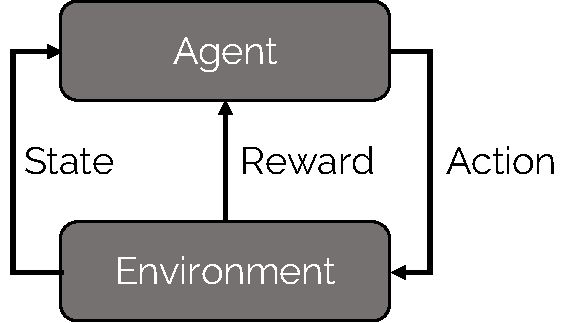
\includegraphics[width=0.3\textwidth]{RL_Fundamentals.pdf}
\caption{General concept of \acrfull{RL} as the interactions between the agent and its environment. The agent takes some action that has an impact on the environment which feeds back the agent with a reward and the new state. The objective of the agent is to optimise its policy, \ie mapping between the state it is at and the action to take, by maximising its cumulative reward.}
\label{fig:RL_Fundamentals}
\end{figure}

The agent learns to optimise its policy by maximising the cumulative reward over time. This policy refers to the strategy or mapping from states to actions that the agent employs to make decisions. Essentially, it defines the behavior of the agent in the environment. The ultimate goal of the agent is often to find an optimal policy, which maximises the expected cumulative reward over time.  All these concepts and interactions between the agent and its environment are formalised as a \gls{MDP} \cite{sutton2018reinforcement}, represented by the tuple $<s,a,T,r,\pi,\gamma>$.  The Markov property of such a decision process states that a decision is made only based on this tuple and not on the history/path that has led to it. In this tuple, $s\in S$ is the state defined in a certain state space, $S$, that represents the observable parts of the environment that the agent uses to make decisions; $a\in A$ is the action among the action space, $A$; $T$ is the probability of transitioning from one state $s$ to another state $s'$ given a specific action, $a$: $T(s,a,s'): \text{Pr}\left(s'|s,a\right)$; $r$ is the reward received by the agent when taking the action $a$ from state $s$, $r(s,a)$; $\pi$ is the policy telling the action to take depending on the current state and; $\gamma$ is the discount factor that controls the importance of future rewards versus immediate rewards. During the learning/optimisation process, the agent acts according to the exploitation-exploration trade-off. In the exploitation, the action $a$ is directly given by the mapping provided by the current policy $\pi$,  depending on the state $s$. In the exploration, the action is randomly picked within the action space. For further information, the interested reader is invited to refer to work of \citet{sutton2018reinforcement} or the course given by \citet{davidsilver_RL_online} available online.

Due to the increasing complexity of the systems and the integration of uncertainties, the last decades have seen the emergence of publications where \gls{RL} is applied to energy systems \cite{cao2020reinforcement,perera2021applications}. In their respective reviews, \citet{cao2020reinforcement} and \citet{perera2021applications} highlighted groups of problems addressed with \gls{RL} in the research field of energy systems: building energy management system (BEMS), optimisation of dispatch and operational control closely linked with the energy market and the optimal power flow problem in the grid, micro-grid management, electro-mobility or even demand-side management or optimal control of energy system devices like maximum power point tracking (MPPT) of wind turbines and \gls{PV} panels.  The major novelty of this thesis is the application of \gls{RL} to a new kind of energy system problem: the optimisation of the transition pathway of a whole-energy system. In this sense, the objective is to optimise a policy to support this transition subject to uncertainties.

\subsection{Problem formulation and algorithm}
\label{subsec:meth_RL_algo}
At the initial state, \ie the energy system in 2020, the agent gets an initial observation, $\bm{o}_0$. An observation represents a set of the characteristics of the environment accessible to the agent for it to take the next action. The state, though, is the exhaustive list of these characteristics. Even though an observation is a subset of the state, this work uses these two words interchangeably. Then, it takes an action, $\bm{a}_0$, impacting its environment, \ie the energy system limited transition over the first decision window (2020-2030). Through this interaction with its environment, the agent is given a reward, $r_1=r\left(\bm{a}_0 | \bm{o}_0 \right)$, and ends up in a new state, \ie the energy system in 2025, characterised by a new observation, $\bm{o}_1$, and so on (see Figure \ref{fig:Schematics_RL}).


\begin{figure}[!htbp]
\centering
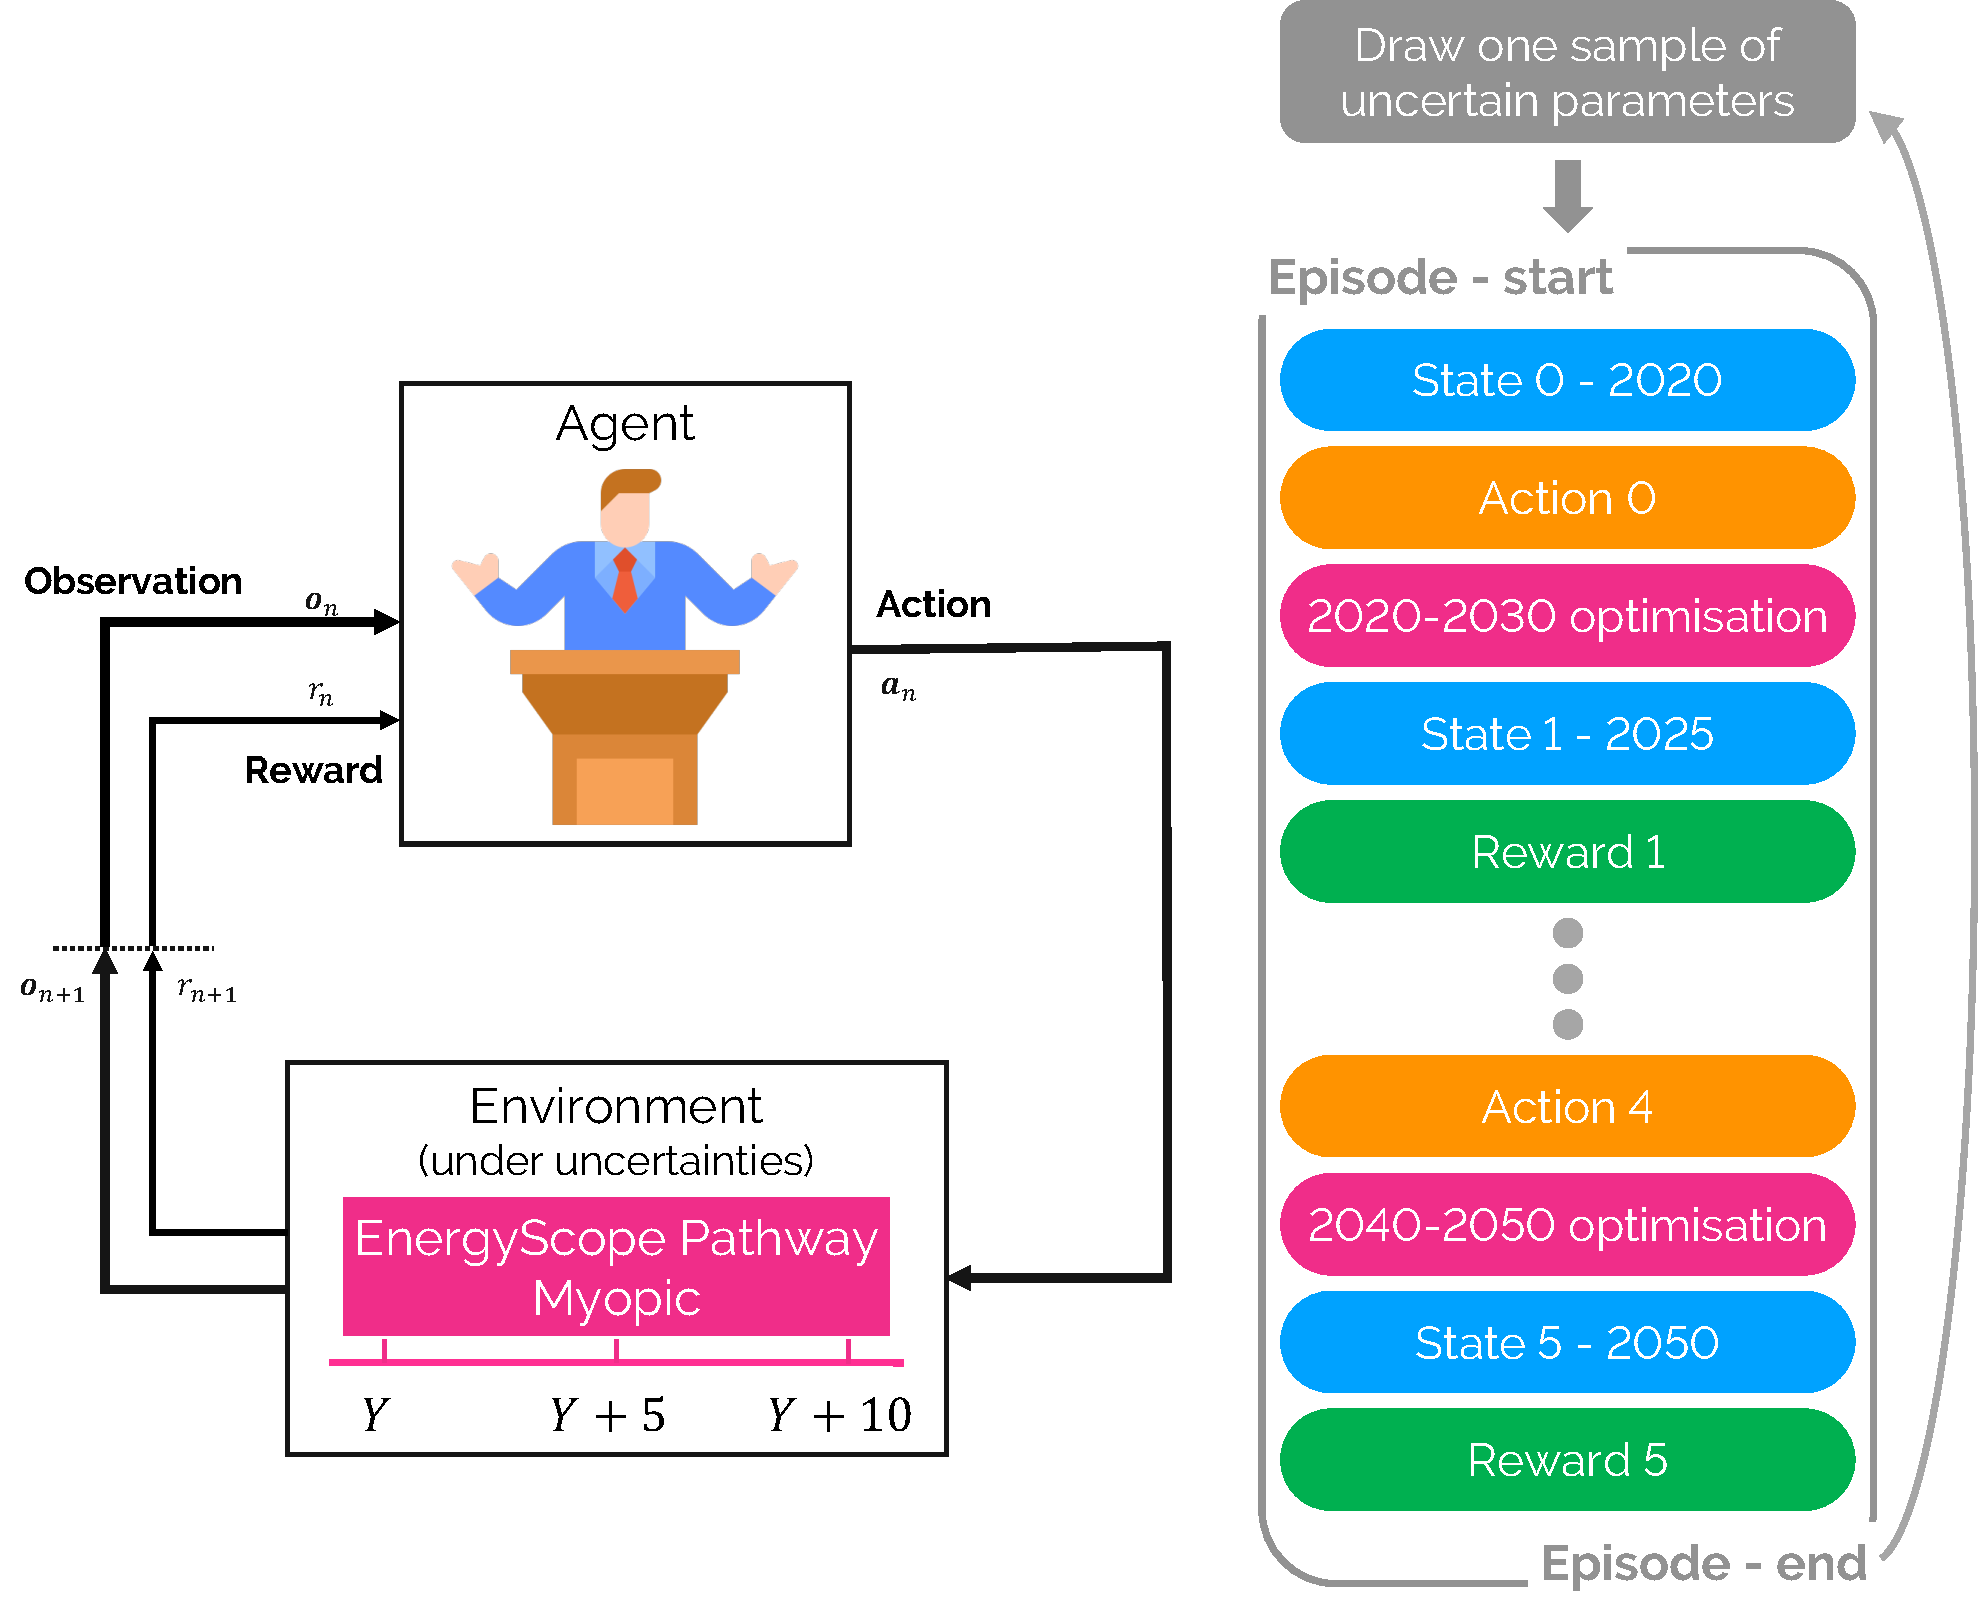
\includegraphics[width=0.8\textwidth]{Schematics_RL.pdf}
\caption{\Acrfull{RL} framework made of the agent interacting with its environment, \ie the energy-system model on a limited decision window of 10 years.}
\label{fig:Schematics_RL}
\end{figure}

A learning episode is a succession of such learning steps. In the context of the transition pathway between 2020 and 2050, an episode can come to an end for different reasons. First, if the actions taken by the agent make the optimisation infeasible, the episode is prematurely stopped before reaching 2050. Similarly, cumulative emissions of the system over the predefined \ce{CO2}-budget (see Section \ref{sec:cs:CO2-budget}) lead to an anticipated end of the episode. Finally, the ``natural'' end is the prescribed end of the transition, \ie 2050. Consequently, the maximum value of steps for an episode is equal to $N=5$. 

\newpage
Before jumping to the choice of the learning algorithm, it is worth noting that we opted for the combination of \gls{RL} with \gls{DNN}, called \gls{DRL}. Among others, one of the main drawbacks of traditional \gls{RL} algorithms, \ie without the use of \gls{NN},  is that it suffers from the ``curse of dimensionality'' when facing problems with continuous action and state spaces (see Chapter \ref{chap:chap_RL}). By approximating the state-action function with its parameters (\ie weights and biases), \gls{DNN} can address this difficulty. 

Given the assumed absence of knowledge of the agent about the dynamics of the environment, \ie its transition or reward functions, we needed a so-called ``model-free'' learning algorithm. In practice, in a model-free approach, the agent estimates the optimal policy directly from experience and without estimating the dynamics of the environment. However, model-free methods suffer from two major drawbacks: their sample inefficiency and their sensitivity with respect to their hyper-parameters (\eg learning rates, exploration constants) \cite{haarnoja2018soft}. The former leads to a too expensive computational burden while the second requires meticulous settings to get good results.  To overcome these two challenges, we needed to chose between an ``on-policy'' or ``off-policy'' algorithm. In a nutshell, in on-policy learning, the agent learns the value function or policy based on the data it generates by following its current policy whereas, in off-policy, the agent can learn from data collected by any policy, not just the one it is currently following, which provides greater flexibility and potential for reusing data stored in the so-called replay buffer. This makes off-policy algorithms more data efficient and ensuring better exploration by reusing past experiences or even following random exploration \cite{haarnoja2018soft}.

To optimise the mapping between the observations and the actions, the policy $\pi\left(\bm{a}_n | \bm{o}_n\right)$, an objective function, $\bm{J}(\pi)$, is built on the cumulative rewards collected during each episode. Finally, a back-propagation process updates the weights and biases of the \gls{NN} during the learning of the agent. Among the wide variety of \gls{RL} algorithms applied in energy systems \cite{perera2021applications}, this work opted for \gls{SAC} \cite{haarnoja2018soft} to train and update the \gls{NN}.  Like other actor-critic-based algorithms, \gls{SAC} works with two \gls{NN} in parallel: the actor learning the control policy and the critic judging the actor (see Figure \ref{fig:Actor-critic}).

\begin{figure}[!htbp]
\centering
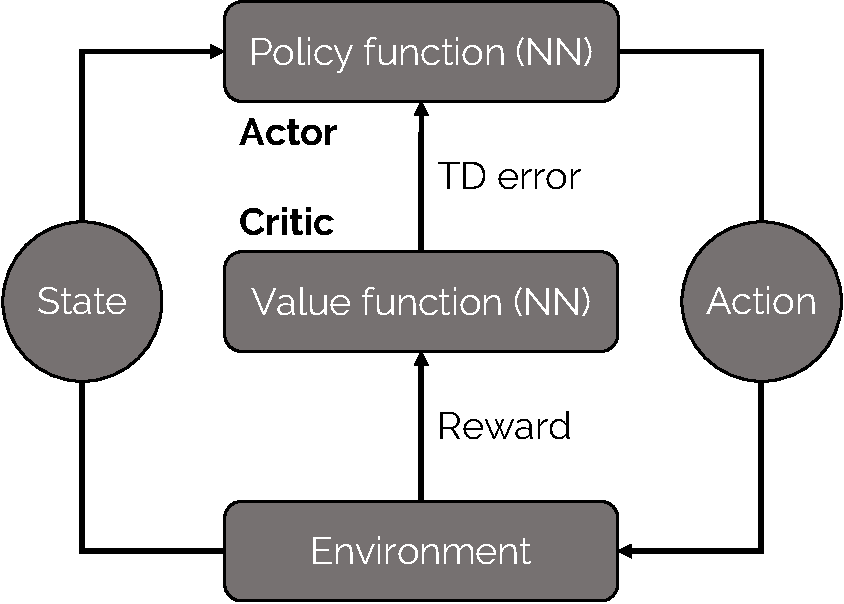
\includegraphics[width=0.5\textwidth]{Actor-critic.pdf}
\caption{General concept of actor-critic-based algorithms. The two \gls{NN} are trained against each other for the actor to improve the control policy and for the critic to provide a better judgement of the actor's action via the temporal-difference (TD) error. Graph adapted from \cite{cao2020reinforcement}.}
\label{fig:Actor-critic}
\end{figure}

\gls{SAC} is a model-free and off-policy actor-critic deep \gls{RL} algorithm based on the entropy-augmented objective function (see Equation (\ref{eq:SAC_objective})). The word ``augmented'' here is in opposition to the conventional \gls{RL} objective function that is only based on the cumulative reward, \ie first term of Equation (\ref{eq:SAC_objective}). In the \gls{RL} context, the entropy, also called ``Shannon entropy'', stands for the randomness or stochasticity of the policy.

\begin{equation}
    \label{eq:SAC_objective}
    \bm{J}(\pi) = \underset{\pi}{\mathbb{E}}\left[\underset{n=0}{\overset{N_{ep}}{\sum}}\gamma^n r_n\left(\bm{o}_n,\bm{a}_n \right) - \zeta \log \left(\pi\left(\bm{a}_n | \bm{o}_n\right) \right) \right],
\end{equation}

\noindent
where $\gamma$ is the discount factor and $\zeta$ the temperature parameter. $\gamma$ determines how much importance we want to give to future rewards within an episode. $\zeta$ balances the trade-off between exploitation of proven actions via the return maximisation, \ie $\sum_{n=0}^{N_{ep}}\gamma^n r_n\left(\bm{o}_n,\bm{a}_n \right)$, and exploration through the entropy term, \ie $\log \left(\pi\left(\bm{a}_n | \bm{o}_n\right) \right)$. This way, \gls{SAC} ensures sample efficiency while improving exploration \cite{haarnoja2017reinforcement} and robustness \cite{ziebart2010modeling}. In their work, \citet{haarnoja2017reinforcement} showed a lower sensitivity of \gls{SAC} to hyper-parameters. These make \gls{SAC} a state-of-the-art algorithm and one of the most efficient model-free deep RL method nowadays \cite{haarnoja2017reinforcement}. In this thesis, we used the open-source \gls{SAC} package developed by \textsc{Stable-Baselines3} \cite{raffin2021stable} where the policy \gls{NN} is a fully connected multilayer perceptron (MLP) built with \textsc{TensorFlow} \cite{abadi2016tensorflow}. For further information on \gls{RL} and the \gls{SAC} algorithm, the interested reader is invited to refer to the works of \citet{sutton2018reinforcement} and \citet{haarnoja2018soft}, respectively.

\section{Robustness assessment via PCA}
\label{sec:meth:PCA}
When optimising a transition pathway of a whole-energy system, including its uncertainties, capturing the variance of design (\ie installed capacities of each technology) can become overwhelming due to the curse of dimensionality. For the case study detailed in Chapter \ref{chap:case_study}, this consists of 113 possibles technologies over 7 representative years. To tackle this challenge, we have developed a methodology based on the \acrfull{PCA}. The philosophy behind this approach is to identify key-combinations of design variables capturing most of the system variance, beyond the sole objective function, \ie total transition cost, but without having to compare each design variable individually. This methodology provides two main outputs. First and foremost, using the model runs necessary to quantify the impact of the uncertain parameters on the total cost of the transition (see Section \ref{sec:meth:UQ}), it gives a metric on which to assess the robustness of different energy transition policies. Where the total transition cost is a single value representing the entire system and analysing individually all technologies would be overwhelming, this metric gives the happy medium. Second, these ``directions of variation'' can highlight key modal shifts or highly varying design strategies over the transition. After introducing the general concept of \gls{PCA}, this section aims at detailing the methodology proposed to obtain these ``directions of variation'' and to assess the robustness of policies.

\subsection{Principal Component Analysis: General concept}
\label{subsec:meth:PCA:PCA}
Born in the early 20th century \cite{pearson1901on,hotelling1933analysis}, the \acrfull{PCA} finds its fundamentals from the \gls{SVD}. \gls{SVD} is a generalisation, to an arbitrary (\ie not necessary square) matrix, of the spectral theorem stating that a normal matrix can be diagonalised by an orthonormal basis of eigenvectors.  The core concept of principal component analysis (PCA) involves simplifying the original dataset with numerous interconnected variables by reducing its dimensionality while preserving as much variability within the data. This is accomplished by transforming the $p$-dimension data, $\mathbf{x}$, into a new set of variables called principal components (PCs), $\mathbf{z}$. These components are uncorrelated and arranged in such a way that the first ones retain the majority of the variability found in the original dataset. On the other hand, the final PCs pinpoint directions where there is minimal variation, indicating nearly constant linear relationships among the original variables \cite{jolliffe2002principal}. 

The PCs are computed based on the covariance matrix of $\mathbf{x}$, $\mathbf{\Sigma}$, where the diagonal of this matrix gives the variance of the $i^{\text{th}}$ variable and the other elements give the covariance between the $i^{\text{th}}$ and the $j^{\text{th}}$ variables where $i\neq j$. Out of this matrix, $\mathbf{\alpha_k}$ is the eigenvector of $\mathbf{\Sigma}$ corresponding to its $k^{\text{th}}$ highest eigenvalue $\lambda_k$. These eigenvectors are orthogonal to each other so that they represent independent directions in the original feature space. These eigenvectors are also normalised such that $\mathbf{\alpha_k}^{T}\mathbf{\alpha_k}=1$ \cite{jolliffe2002principal}, where $\mathbf{^T}$ means the transpose vector. This makes it easier to interpret the relative importance of each principal component in explaining the variability of the data. Finally, this ensures a fair comparison between the original features. Without normalization, variables with larger scales would dominate the principal components, potentially skewing the results and leading to misinterpretation of the principal components. In other words, given this normalization, $\mathrm{var}\left(z_k\right)=\lambda_k$, where $\mathrm{var}\left(z_k\right)$ is the variance of $z_k$. Moreover, this means that the coefficient $\alpha_{ki}$, \ie the component of $ \mathbf{\alpha_k}$ related to the $i^{\text{th}}$ original variable, $x_i$,  gives its weight in the $k^{\text{th}}$ PC, \ie $z_k$. This PC captures $\lambda_k$ variance of the original data. In other words, a high absolute value of $\alpha_{ki}$ means that $x_i$ has a significant impact in the direction given by the $k^{\text{th}}$ PC \cite{zdybal2022advancing}. 

Easier to represent in two dimensions, let us consider a vector $\mathbf{x}$ composed of the variables $x_1$ and $x_2$, $p=2$, and 25 realisations of them (See Figure \ref{fig:PCA_intro_original}). 

\begin{figure}[!htbp]
\centering
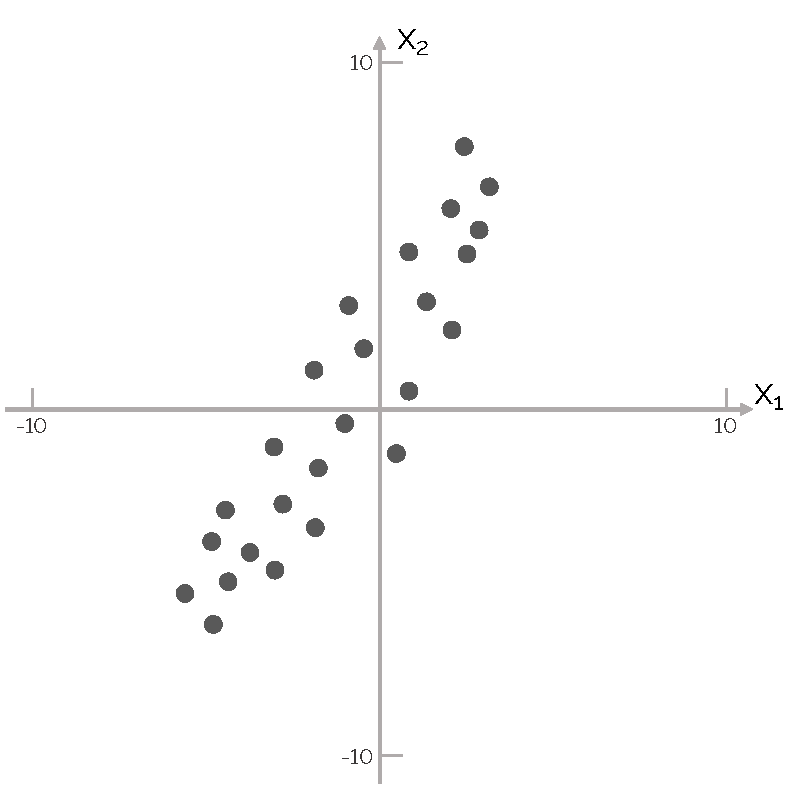
\includegraphics[width=0.4\textwidth]{PCA_intro_original.pdf}
\caption{Original observations of a two-dimension dataset, $x_1$ and $x_2$.}
\label{fig:PCA_intro_original}
\end{figure}

From these observations, the main objective of \gls{PCA} is to find the linear combination, \ie projection, of the original variables that maximise their spread, \ie variance (see Figure \ref{fig:PCA_intro_proj}).  Another way to understand this is to look at the other side of the same coin. Indeed, \gls{PCA} also looks for properties that allow reconstructing the original features as accurately as possible. In practice, it aims at minimising the total reconstruction error that is the average squared distance between the original observations and their respective projection. 

\begin{figure}[!htbp]
\centering
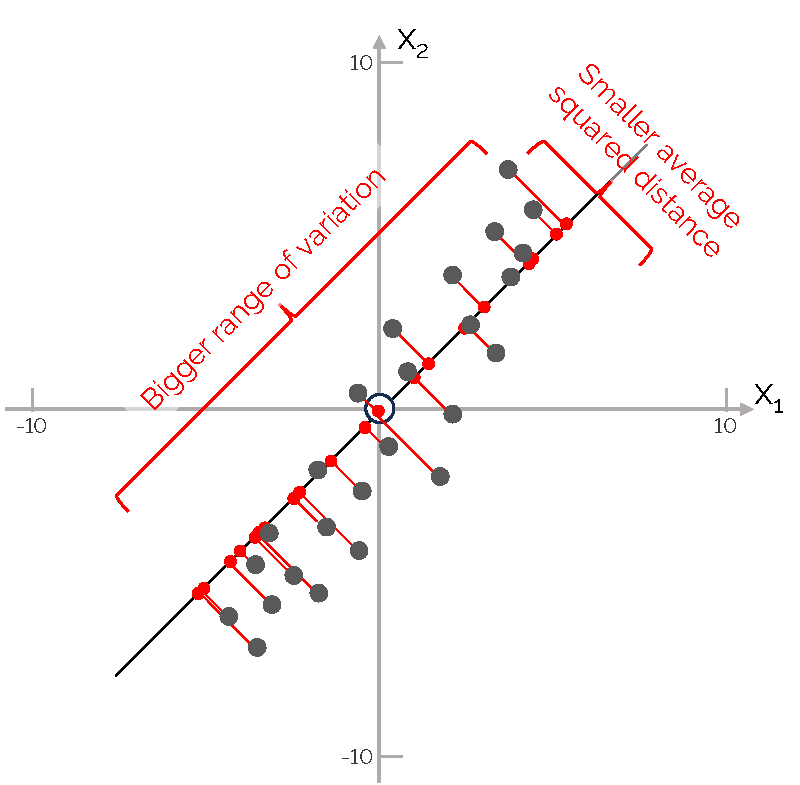
\includegraphics[width=0.4\textwidth]{PCA_intro_proj_1.pdf}
\hspace{1.5cm}
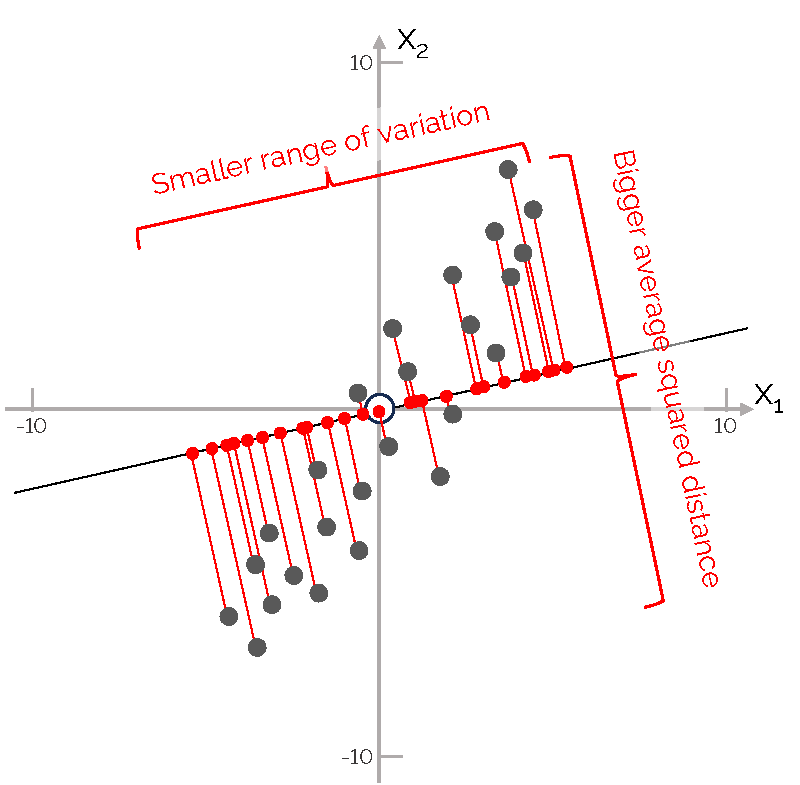
\includegraphics[width=0.4\textwidth]{PCA_intro_proj_2.pdf}
\caption{Two different projections (red dots) of the original observations (grey dots). Projection on the left captures a bigger variance than the projection on the right. At the same time, the average squared distance between the original observations and their respective projection is smaller for the projection on the left. Consequently, the left projection is closer to be the first PC than to the right projection.}
\label{fig:PCA_intro_proj}
\end{figure}

Mathematically, the first \gls{PC}, $z_1$, is a linear function, $\mathbf{\alpha_1^{T}x}$,  of the different variables of $\mathbf{x}$ with maximum variance:

\begingroup
\belowdisplayskip=2pt
\abovedisplayskip=2pt
\begin{flalign}
\hspace{0pt}
  \label{eq:PCA_z1}%7
 z_1=\sum_{j=1}^{p} \alpha_{1j}x_j=\mathbf{\alpha_1^{T}x}=\alpha_{11}x_1+\alpha_{12}x_2.
\end{flalign}
\endgroup

\noindent
Then, $z_2=\mathbf{\alpha_2^{T}x}$, is another linear function of $\mathbf{x}$, uncorrelated with $z_1$ and capturing the remaining variance. These linear transformations can be seen as projection of the original data on the principal direction, \ie PCs (see Figure \ref{fig:PCA_intro_PCA}).

In the general cases of $p$ original variable, one can write $z_k=\mathbf{\alpha_k^{T}x}$ as the $k^{\text{th}}$ PC. There can be up to $p$ PCs even though, usually, most of the variance of the original data can be captured by $m$ PCs where $m\ll p$. The interested reader is invited to refer to the work of \citet{jolliffe2002principal} for further mathematical demonstrations, information and examples.

\begin{figure}[!htbp]
\centering
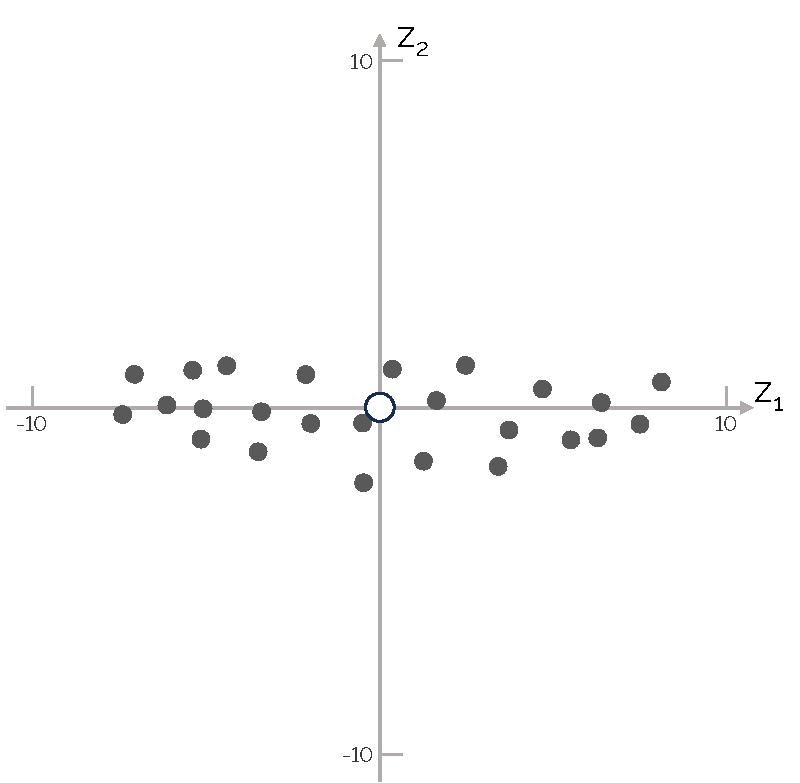
\includegraphics[width=0.4\textwidth]{PCA_intro_PCA.pdf}
\caption{Projection of the original observations with respect to their PCs. The variation of the realisations was more significant in the direction of $x_2$ than $x_1$. Once projected with respect to their PCs, the variation is even more significant in the direction of $z_1$ than in either of the original variables, as it captures most of their variance. }
\label{fig:PCA_intro_PCA}
\end{figure}

\subsection{Principal components of the transition}
\label{subsec:meth:PCA:transition}
As introduced, the objective is to define the main technological drivers of the variation through the transition to 2050 subject to uncertainties. To do so, before calculating the PCs of the transition, three preliminary steps are necessary: (i) selection of the right data, (ii) data scaling and, (iii) outliers management. Like any other dimension-reduction process, \gls{PCA} has to be supplied with relevant data to reach the stated objective.  Like the normalization of the eigenvectors (see Section \ref{subsec:meth:PCA:PCA}), data scaling is fundamental to compare features having potentially different units and/or order of magnitude. Then, properly handling the outliers allows reaching the relevant level of metric between the too vague information of the sole total transition cost and too many details hidden in the peculiar/outlying cases. After this preprocessing, PCs can be computed for each of the representative year of the transition. Finally, PCs that indicate similar directions in different years are averaged into one single PCs of transition. The different PCs of transition give a bigger picture over the whole transition.\\

\myparagraph{Data selection}\\

\noindent
To characterise the variations of design within the transition under uncertainties, we have focused on the installed capacities, $\textbf{F}(y,j)$ for all $y \in \text{\emph{YEARS}}$ and $j \in \text{\emph{TECH}}$ (see Equation (\ref{eq:F_newBuilt})). Even though these represent only the design part of the result of the optimisation, focusing on the installed capacities gives a direct information regarding the required capital investments (see Equation (\ref{eq:CAPEX_v2})) and, more indirectly, the operation. In other words, it captures the technological landscape of the transition.  Having defined the type of variable to consider, we need to assemble a relevant dataset. This is given by the runs to quantify the impact of the uncertain parameters on the total cost of transition required by the method described in Section \ref{sec:meth:UQ}. Overall, the original dataset is $\textbf{x}(y,j,s)$ where, on top of $y$ and $j$ previously defined, $s \in [1,2,...,S]$ stands for the sample number of the uncertainty quantification method. For the investigated case detailed in Chapter \ref{chap:atom_mol}, this represents $S=1260$ samples resulting from the perfect foresight optimisation of the transition pathway under uncertainties. Appendix \ref{app:UQ_tech_cap} gives the distribution of the installed capacities among the different end-use sectors from the \gls{GSA}. Finally, among the seven representative years of the transition, we do not consider 2020 as it is the initialisation year for which the design of the system is fixed, to be representative of the actual design that was in place in Belgium in 2020 (see Appendix \ref{app:bel_2020}). In other words, we focus here only on the years 2025, 2030, 2035, 2040, 2045 and 2050. This gives the whole dataset considered in this \gls{PCA} (see Figure \ref{fig:PCA_data}). \\

\begin{figure}[!htbp]
\centering
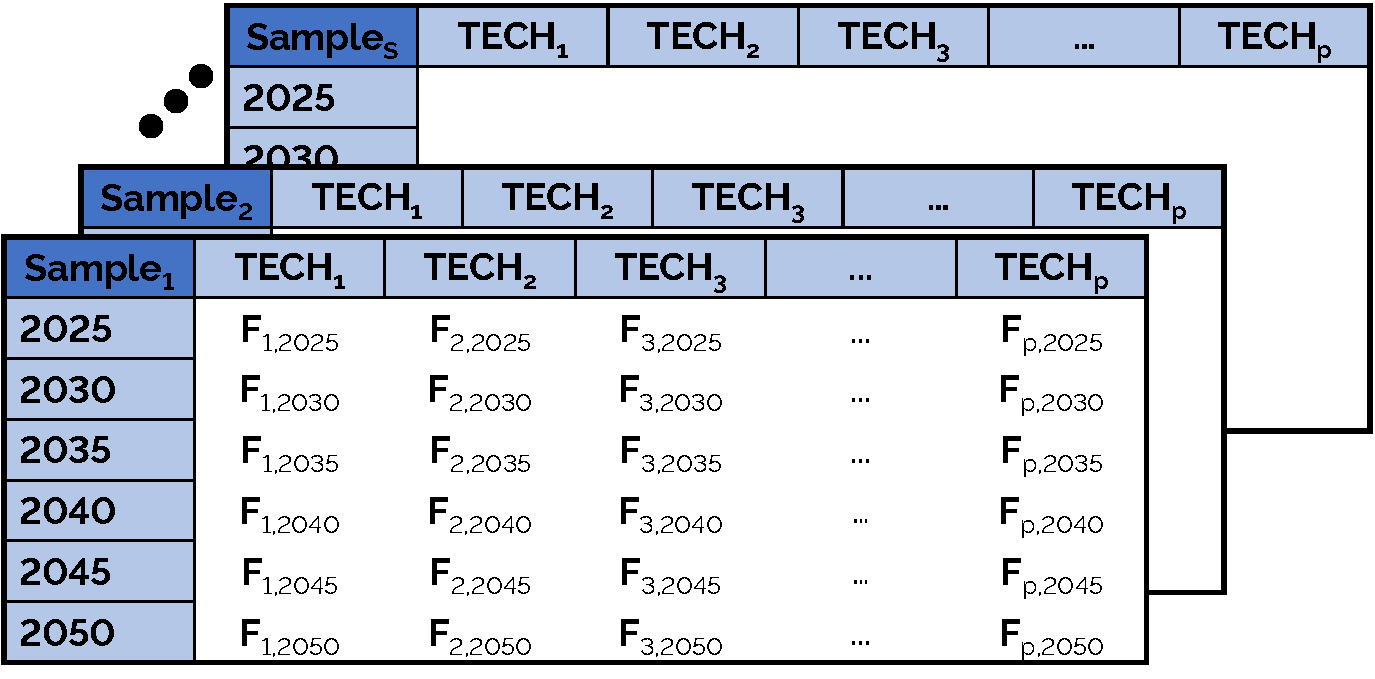
\includegraphics[width=0.8\textwidth]{PCA_data.pdf}
\caption{Original raw data considered in the \acrfull{PCA} of the variation of the design strategy through the transition, $\textbf{x}(y,j,s)$, accounting for the $p$ possible technologies to install.}
\label{fig:PCA_data}
\end{figure}

\myparagraph{Data scaling}\\

\noindent
Preprocessing the dataset before employing a method to reduce dimensionality, like \gls{PCA}, can greatly affect the structure of the simplified representation and the characteristics of the features extracted from the dataset \cite{parente2013principal,peerenboom2015dimension}. Scaling the original raw data via normalization, \ie reducing data to $[0, 1]$ interval has a double purposes: to assess variables (i) representing different sorts of features, with different units (\eg installed capacity of electricity and mobility technologies) and, (ii) ranging over the different orders of magnitude (\eg installed capacity of private and public mobility) (see Appendix \ref{app:bel_2020}).  Consequently, the first part of this data preprocessing consists in scaling the installed capacities versus their respective sector and representative year (see Equation (\ref{eq:PCA_scaling_0})). The sectors, as defined in EnergyScope, are the electricity, \gls{HT} heat, \gls{LT} heat, passenger mobility, freight mobility, \gls{NED}, storage and infrastructures. For instance, the installed capacity of \gls{PV} panels in the year $y$ of the sample $s$ is scaled by the maximum installed capacity in the electricity sector in the year $y$ among all the samples.

\begin{equation}
 \label{eq:PCA_scaling_0}
\textbf{x}^{*}(y,j,s)=\frac{\textbf{x}(y,j,s)}{\mathrm{max}_{sec,y}\left(\textbf{x}(y,j,s)\right)}
 \quad \forall y \in \text{\emph{YEARS}}, sec \in \text{\emph{SECTORS}}
\end{equation}

Then, to give ``directions/metrics'' representative to the size of each sector within the energy system, we added another weight based on the relative share of commodity produced by each sector. For the case study of Belgium detailed in Chapter \ref{chap:case_study}, this gives a higher weight for electricity and low-temperature heat sectors (see Figure \ref{fig:Share_EUD_sectors}). 

\begin{figure}[!htbp]
\centering
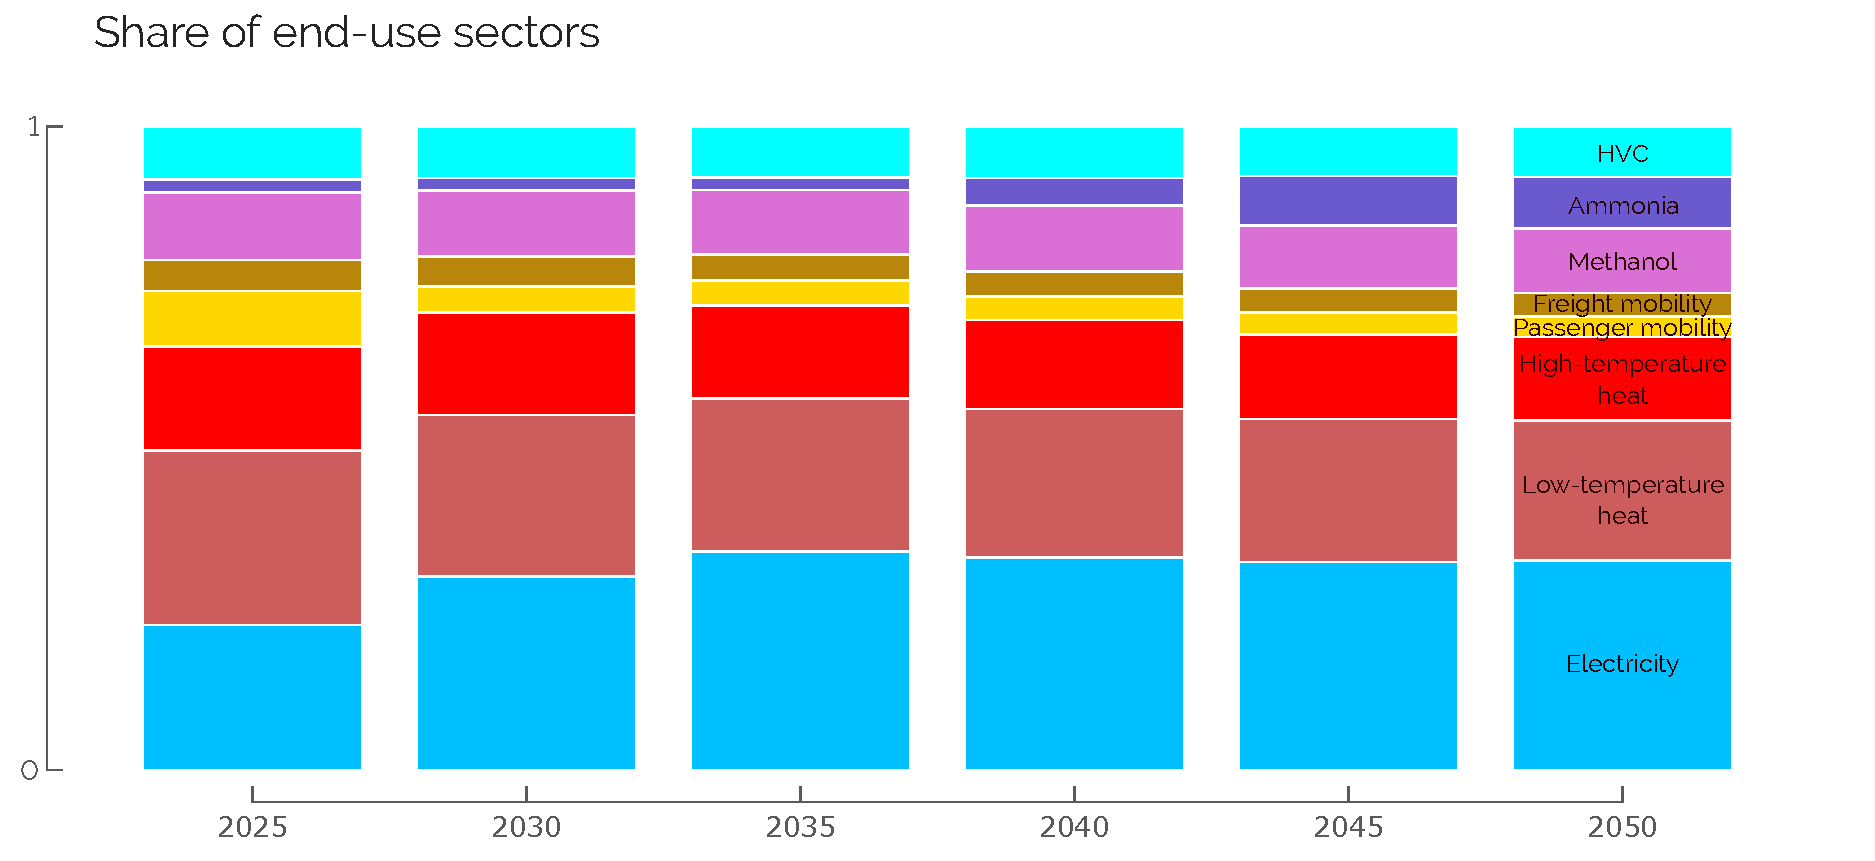
\includegraphics[width=1\textwidth]{Share_EUD_sectors.pdf}
\caption{Multiplying factor for each of the end-use sectors in the case of Belgian energy transition. These shares are based on results of the reference scenario (REF) where nominal values are considered for the uncertain parameters and the transition is optimised through the perfect foresight approach. Over the transition, sectors like electricity (\ie from 22\% in 2025 to 33\% in 2050) or ammonia (\ie from 2\% to 8\%) become more important due to sector coupling, \eg e-mobility or ammonia-\gls{CCGT}.}
\label{fig:Share_EUD_sectors}
\end{figure}

To do so, we have arbitrarily considered these shares from the REF case, where the pathway is optimised according to the perfect foresight approach and considering all the uncertain parameters to their nominal values (see Chapter \ref{chap:atom_mol}).  The end-use-demands as well as the commodity produced for the sector coupling are based on the results of this deterministic REF case.  For instance, the share of the electricity sector accounts for its \gls{EUD} and the electricity produced to supply other sectors (\eg heat, mobility). Finally, to compare apples with apples, we converted the \gls{EUD} in the mobility sectors, \ie passenger and freight, into the \gls{FEC} they require in the REF case. This gives the second weighing factors to scale data, on top of the ones of Equation (\ref{eq:PCA_scaling_0}), see Equation (\ref{eq:PCA_scaling_1}).

\begin{equation}
 \label{eq:PCA_scaling_1}
\textbf{x}^{**}(y,j,s)=\textbf{x}^{*}(y,j,s)\cdot \text{share}_{\text{EUD}}(y,sec)
 \quad \forall y \in \text{\emph{YEARS}}, sec \in \text{\emph{SECTORS}}
\end{equation}

One can notice that this second scaling factor omits the infrastructure and storage technologies. In the process to define ``metrics'' to assess the robustness of a policy for the case of Belgium, this has a negligible impact. Indeed, the variation of the installed capacity of these technologies are either limited compared to end-use-type (EUT) technologies, \ie limiting their influence in the definition of PCs, or directly linked to these EUT technologies. For instance, \gls{DHN} installed capacity is directly proportional to technologies producing \gls{LT} heat in \gls{DHN} or the additional capacity of grid is caused by additional capacities of \gls{VRES}. \\

\myparagraph{Outliers management}\\

\begin{wrapfigure}{r}{3cm}
\centering
\captionsetup{justification=centering}
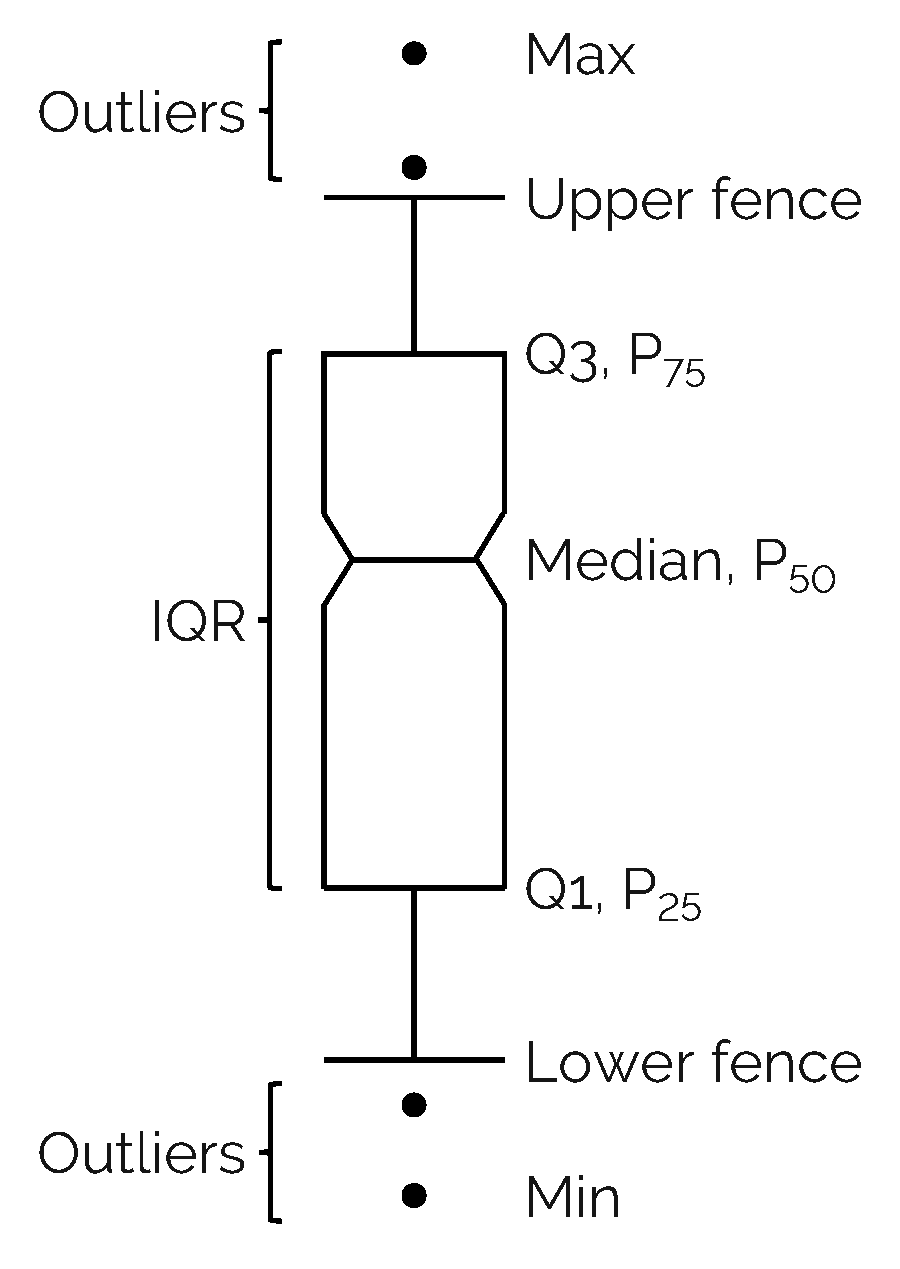
\includegraphics[width=2.8cm]{Schematic_boxplot.pdf}
\caption{}
\label{fig:Schematic_boxplot_methodo}
\end{wrapfigure}

\noindent
Handling outliers is one of the biggest challenges in data science \cite{aguinis2013best}. These are defined as data points differing significantly from the rest of the data set. Being extreme values, outliers influence the overall dataset variance and, consequently, rotate the PCs directions towards them \cite{stanimirova2007dealing}. In the context of \gls{PCA}, outliers could be defined as ``model fit outliers'' as their presence influences the fit of the model. There are several techniques to detect/define and handle the outliers \cite{aguinis2013best}. In this work, detection is performed via the box plot technique, as outliers are identified as those points lying beyond the plot’s whiskers, or fences. These whiskers are themselves constructed as being 1.5 times the \gls{IQR} (Q3 - Q1) higher or lower than the third (Q3) or first quartile (Q1), respectively (see Figure \ref{fig:Schematic_boxplot_methodo}). Therefore, the installed capacity of a technology in the year $y$ of the sample $s$ is defined as an outlier if it falls out of this range compared to the dataset for this specific technology and year. There exist several techniques to handle these outliers depending on their nature or the method used to identify them. Since all the data points correspond to a result provided by the optimisation, we have decided to keep these points but carry out a ``modification'' of them \cite{aguinis2013best}. In practice,  the value of ``high outliers'' or ``low outliers'' is set to the upper or lower fence, respectively. In practice, this modification narrows the variation range of features presenting outliers and, consequently, reduces their weight in the different PCs.\\

\myparagraph{Principal components of each representative year}\\

\noindent
Now that data are selected and preprocessed, principal components are first computed for each representative year separately, using the Python package \textsc{PCA} from \textsc{sklearn.decomposition}. As explained in Section \ref{subsec:meth:PCA:PCA}, the number of PCs per year to retain can go up to the number of considered variables (\ie 73 in our case study\footnote{73 technologies out of the 113 in total as we do not consider the 15 infrastructure technologies nor the 25 storage technologies.}) which is intractable. Moreover, the first PCs keep track of most of the variance of the system whereas the last ones present a smaller interest. Choosing the appropriate threshold involves a trade-off. Retaining too few principal components may result in loss of important information, while retaining too many may lead to unclear analysis. For each of the representative years of the transition (except 2020), we compute the PCs that capture 90\% of the total variance of this year \cite{jolliffe2002principal}. At the end of this step, a list of $m$ PCs is obtained, \ie $\text{PC}_{y,i}$ where $y$ stands for the representative year between 2025 and 2050 and 

\begin{equation}
\label{eq:PC_year}
\sum_{i=0}^m\text{var}\left(\text{PC}_{y,i}\right)\geq 90\% \sum_{i=0}^p\text{var}\left(\text{PC}_{y,i}\right) \quad \forall y \in \text{\emph{YEARS}},
\end{equation}

\noindent
where $m$ is presumably different for each representative year and $p$ is the total number of variables, hence the maximum number of PCs. For the entire transition, it gives a total of $M=34$ $\text{PC}_{y,i}$.\\

\myparagraph{Principal components of the transition}\\

\noindent
The final step consists in defining metrics on the whole transition based on the $\text{PC}_{y,i}$ computed for each representative year, separately. To do so, all the $\text{PC}_{y,i}$ from every year are sorted together in a descending order based on their respective variance. Then, starting with the one with the highest absolute variance, all the other $\text{PC}_{y,i}$ similar to it are clustered together. The similarity between two PCs is defined according to the cosine similarity approach, especially appropriate in high-dimensional positive spaces \cite{xia2015learning}. Indeed, as detailed in Section \ref{subsec:meth:PCA:PCA}, a PC represents a vector for which the components are related to each variable of interest. Therefore, in this work, PCs are considered similar if their cosine similarity, $S_C (A,B)$, is either greater or equal to 90\% or lower or equal to -90\% (see Equation (\ref{eq:cos_similarity})). It is important to consider the second case as \gls{PCA} gives the magnitude of variation within the original feature space via the components of the eigenvectors, regardless of the direction of these vectors. For instance, in a two-dimension original space, if the first PC has $(\sqrt{2}/2;\sqrt{2}/2)$ as eigenvector, this could also be $(-\sqrt{2}/2;-\sqrt{2}/2)$. The second vector being the opposite of the first, they are considered as equivalent in the regard of \gls{PCA}.

\begin{equation}
\label{eq:cos_similarity}
S_C (A,B):= \cos(\theta) = {\mathbf{A} \cdot \mathbf{B} \over \|\mathbf{A}\| \|\mathbf{B}\|} = \frac{ \sum\limits_{i=1}^{n}{A_i  B_i} }{ \sqrt{\sum\limits_{i=1}^{n}{A_i^2}} \cdot \sqrt{\sum\limits_{i=1}^{n}{B_i^2}} } \geq 90\%\text{ or } \leq -90\%,
\end{equation}

\noindent
where $A$ and $B$ represent two different PCs.  The components of these similar PCs are then averaged to form the first PC of the transition, $\text{PC}_{\text{transition},1}$. Then, the process repeats with the next $\text{PC}_{y,i}$ with the highest absolute variance but that has not been integrated in the construction of $\text{PC}_{\text{transition},1}$, to form $\text{PC}_{\text{transition},2}$. This goes on until the sum of the absolute variance of the $N$ $\text{PC}_{y,i}$ used to construct these $\text{PC}_{\text{transition}}$ is greater or equal to $\alpha$\% of the sum of the absolute variance of all the $M$ $\text{PC}_{y,i}$, \ie the ``total transition variance'', generated at the previous step:

\begin{equation}
\label{eq:PC_transition}
\sum_{i=0}^N\text{var}\left(\text{PC}_{y,i}\right)\geq \alpha\% \sum_{i=0}^M\text{var}\left(\text{PC}_{y,i}\right)
\end{equation}

In our case, we have decided to set the value of $\alpha$ to 85\% as, beyond this value, the marginal gain of captured variance becomes too ``costly'' with regard to the number of $\text{PC}_{\text{transition}}$, \ie the level of details, to account for (see Figure \ref{fig:PC_y_share_tot_var}).  Besides being the metrics to assess the robustness of roadmap, these $\text{PC}_{\text{transition}}$ also point out the technologies that are more sensitive to uncertainties and are more likely to impact the overall variance of the transition design.

\begin{figure}[!htbp]
\centering
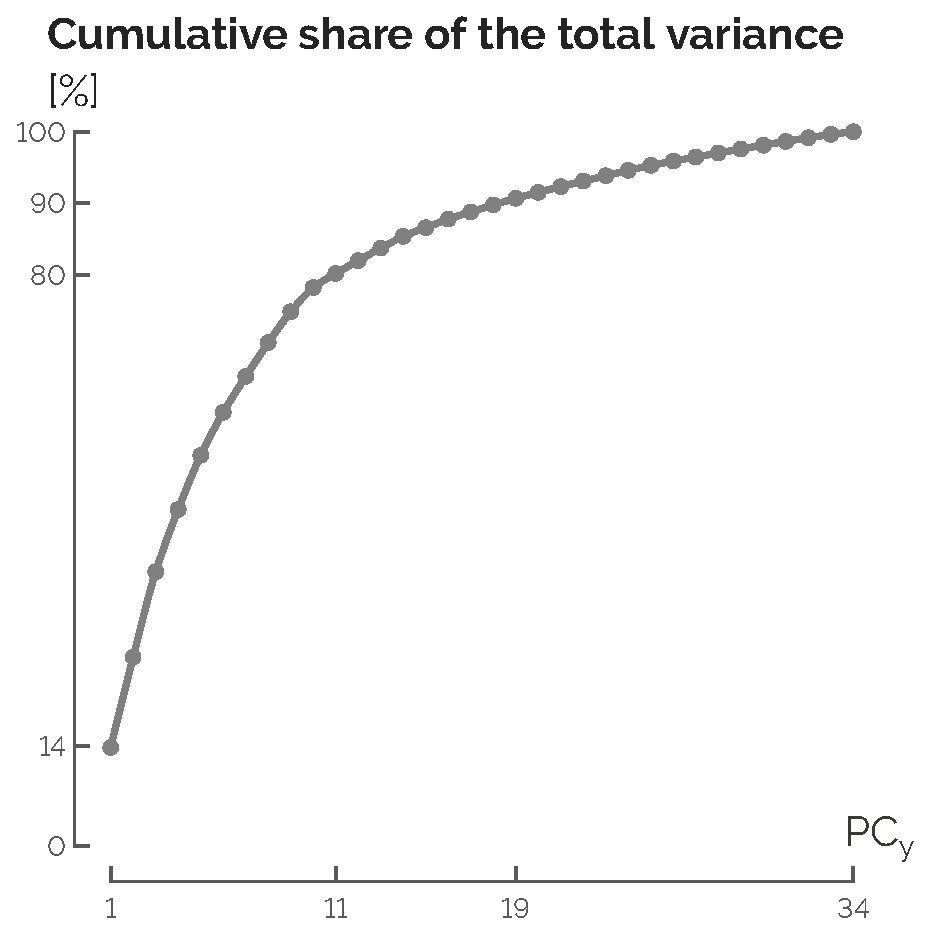
\includegraphics[width=0.5\textwidth]{PC_y_share_tot_var.pdf}
\caption{Cumulative share of the sum of the transition variance versus the number of $\text{PC}_{\text{transition}}$. Passing a certain threshold, here 85\%, the number of $\text{PC}_{\text{transition}}$ to consider increase significantly compared to the share of transition variance that they capture.}
\label{fig:PC_y_share_tot_var}
\end{figure}

\newpage
\myparagraph{Robustness assessment of roadmaps}\\

\noindent
In their analysis, \citet{moret2020overcapacity} assessed the additional capacities after the realisation of uncertainties, the so-called \textit{possibility of recourse} \cite{grossmann2016recent}. These adaptations from the initial investments lead to overcapacity where assets are built but not used because the values taken by uncertain parameters make them cost inefficient. To address the same question of overcapacity in the context of energy transition pathway with progressively revealed uncertainties, we have adapted the method of \citet{moret2020overcapacity} (see Figure \ref{fig:Methodo_Robustness}). Roadmaps are defined by setting minimal installed capacities based on the results of different transition pathway optimisations. The $\text{PC}_{\text{transition}}$ are the metrics on which the results from the myopic pathway optimisation subject to minimal installed capacities set by these roadmaps are projected. 

\begin{figure}[!htbp]
\centering
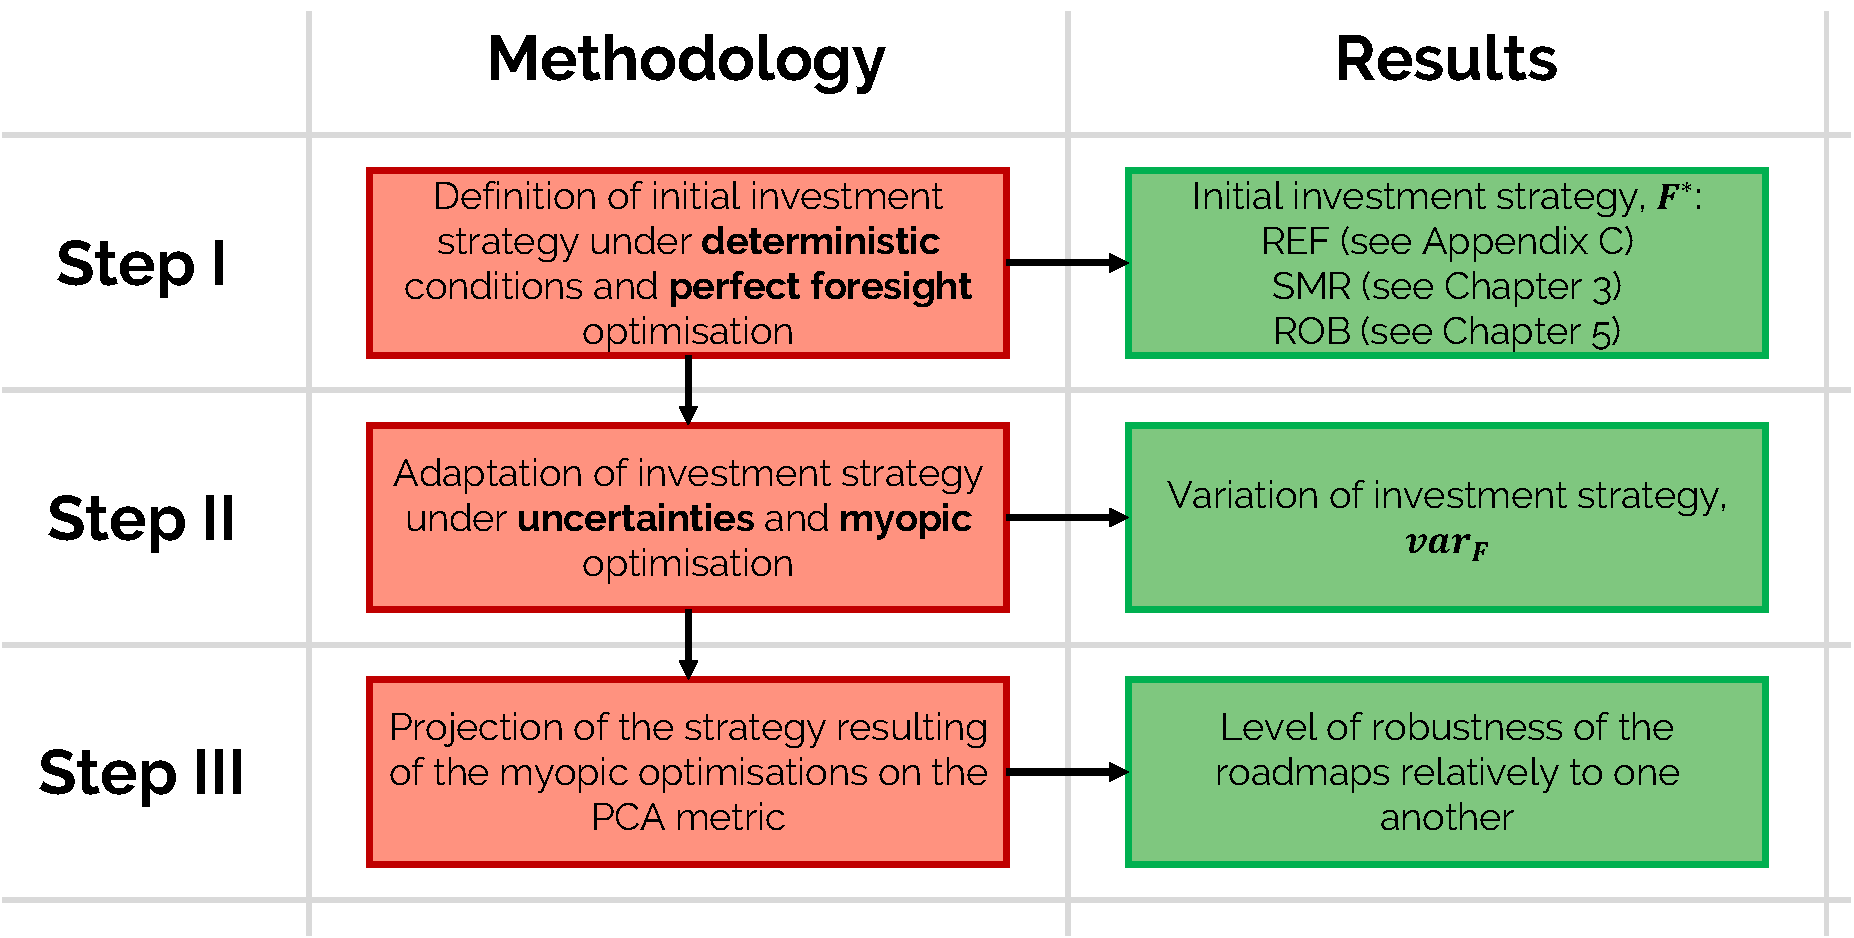
\includegraphics[width=0.8\textwidth]{Methodo_Robustness.pdf}
\caption{Overview of the three-step methodology to assess the robustness of roadmaps. Schematic adapted from \cite{moret2020overcapacity}.}
\label{fig:Methodo_Robustness}
\end{figure}

In conclusion, a roadmap would be defined as more robust than another one if the projection of its myopic runs on the different $\text{PC}_{\text{transition}}$ spans on a more narrow range (see Figure \ref{fig:Projection_PC_transition}). The bounds of this ``range of projection'' are computed as the mean, $\mu$, of the projected data $\pm$ a 95\% confidence level, CL, on the margin of error, MOE:
$$
\text{range of projection} = [\mu-\mathrm{MOE}; \mu + \mathrm{MOE}],
$$

\noindent
where the margin of error, MOE,  is computed thanks to standard error of the mean, SEM, and assuming a Student's, distribution, t,  of the $N$ projected data:
$$
\text{MOE} = \mathrm{SEM}\cdot \mathrm{PPF}_{\mathrm{t}}\left((1+\mathrm{CL})/2,N-1\right),
$$

\noindent
where $\mathrm{PPF}_{\mathrm{t}}$ is the percent point function (\ie inverse of cumulative distribution function) of the Student's distribution.

\begin{figure}[!htbp]
\centering
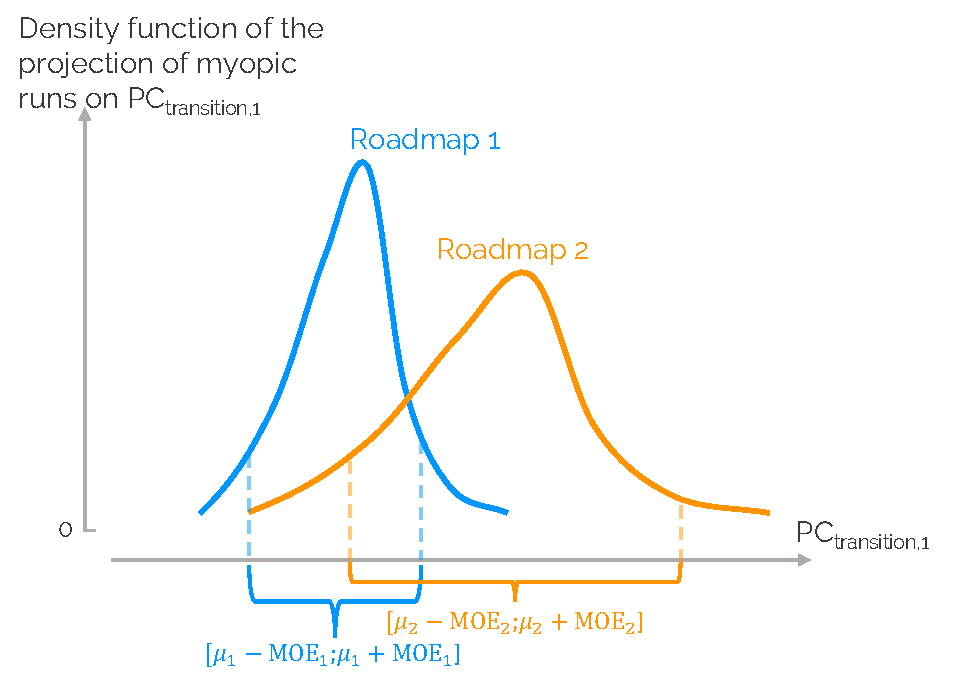
\includegraphics[width=0.65\textwidth]{Projection_PC_transition.pdf}
\caption{Projection on the first PC of the transition, $\text{PC}_{\text{transition},1}$, of the different myopic runs under uncertainties based on different roadmaps. Given that the distribution resulting from roadmap 1 spans over a more narrow range of this PC of the transition, we conclude that this roadmap is more robust than roadmap 2 according to the direction of variation described by $\text{PC}_{\text{transition},1}$.}
\label{fig:Projection_PC_transition}
\end{figure}


\clearpage


%% -- Chapter 2 - UQ on a snapshot model, assessment of electrofuels ---------------------------------
%\chapter{Electrofuels and uncertainties in a target future year}
%\label{chap:chap_electro_uq}
%%!TEX root = ../thesis_main.tex
%!TEX encoding = UTF-8 Unicode

In this chapter aims at showing the first step of uncertainty quantification and highlight a first insight in terms of impacting parameters. It'd also highlight that depending on the gwp\_limit 
\section{From a cost-optimised to a carbon-neutral Belgian energy system: progressive defossilisation}
\label{sec:chap_2_ses_sec2}
In this section, I'd include the section 2 of the electrofuels+UQ paper (\url{https://www.mdpi.com/1996-1073/14/13/4027})(without 2.2 where I presented EnergyScope that I'd include in Chapter 1).

\subsection{Electrofuels}
\label{subsec:chap2_electrofuels}
This section would be as the section 2.1 of the electrofuels+UQ paper (\url{https://www.mdpi.com/1996-1073/14/13/4027}), where I present more specficially how electrofuels are implemented in the model

\subsection{Reference Case Study: The Belgian Energy System in 2050}
\label{subsec:chap2_case_study}
Basically section 2.3 of the electrofuels+UQ paper (\url{https://www.mdpi.com/1996-1073/14/13/4027}), where I present more specficially how electrofuels are implemented in the model where I present what a cost-optimised (without gwp-constraint) Belgian energy system would look like

\subsection{A step by step defossilisation of the snapshot system}
\label{subsec:chap2_defossilisation}
As in section 2.4, quickly show how we implement the defossilisation without having an entire pathway.

\section{Results}
\label{sec:chap2_results}
Similar to Section 4 of the electrofuels+UQ paper (\url{https://www.mdpi.com/1996-1073/14/13/4027}). There'll be work to generate up-to-date results as the model evolved (no more FC\_cars but BEV, for instance)
\subsection{Statistical analysis of the cost}
\label{subsec:chap_2_stat_analysis}

\subsection{Critical parameters}
\label{subsec:chap_2_crit_param}

\section{Discussion and perspective with the literature}
Similar to section 5.1 of the electrofuels+UQ paper (\url{https://www.mdpi.com/1996-1073/14/13/4027})

%\clearpage

%% -- Chapter 3 - Case study -----------------------------
\clearemptydoublepage
\chapter{Case study: the Belgian energy system} 
\label{chap:case_study}
%\begin{flushright}
%%%\emph{``For the things we have to learn before we can do them, we learn by doing them.''}\\%Each wrong scenario you have analysed, is a wrong decision you won't made.''}\\
%%%Aristote
%\emph{All models are wrong, but some are useful.}\\
%George P. Box
%\end{flushright}

%\medskip
%
%\begin{mybox}{Chapter overview}
%\begin{itemize}[left=0em]%[leftmargin=0cm,itemindent=.5cm,labelwidth=\itemindent,labelsep=0cm,align=left]
%\setlength\itemsep{-0.3em}
%\item Belgian energy system overview%Case studies: the Belgian energy systems during the transition (2015-2050).
%\end{itemize}
%\vspace{-0.3cm}
%
%\emph{This chapter is an improved and extended case study version of \citet{Limpens_belgian_2020}}.
%\end{mybox}
%
%\medskip

As detailed by \citet{limpens2024pathway}, the analysis carried out in this work can be applied to any regional whole-energy system. As a densely-populated and highly-industrialised country with limited local renewable potentials (\ie mainly solar and wind representing up to 50\% of the primary mix by 2050), the transition of Belgium from a fossil-dominated system in 2020 (Appendix \ref{app:bel_2020}) to carbon-neutrality in 2050 makes it an intricate case study. Moreover, this case study and the subsequent analyses can be transferred - to some extent - to other industrialised countries highly dependent on fossil fuels with limited local renewable potentials (\eg the Netherlands or Germany) \cite{dommisse2020modelling}. This chapter presents the different demands to satisfy, with a particular focus on the non-energy demand, as well as the resources available and the conversion technologies to supply those. For a comprehensive understanding and detailed descriptions of the technologies, please refer to the documentation \cite{readthedocs_pathway}. Then, the uncertainty ranges considered for some of the parameters are detailed. Finally, the \ce{CO2}-budget over the 2020-2050 transition is presented.

\section*{Contributions}
\label{sec:cs:contributions}
First, as pointed out by \citet{rixhon2022integration}, where most of the studies assessing whole-energy system integrate energy demands (\ie electricity, heart and mobility), the \acrfull{NED} is often not considered. The latter is defined as ‘\textit{energy products used as raw materials in the different sectors; that is not consumed as a fuel or transformed into another fuel}’ \cite{Eurostat2019}. The previous analyses carried out with \gls{ESTD} considered the non-energy demand as the related primary energy needs, \ie either natural gas or \gls{LFO}. To minimise the total cost of the system, the model simply selected the cheapest between the two resources (\ie natural gas). This work goes one step further and accounts for the \gls{NED} as a demand of three commodities (\ie \gls{HVC}, ammonia and methanol) as well as with associated production technologies. This allows bringing the non-energy sector to a similar level of details as the other sectors.  Keeping the same methodology to define \gls{EUD} in EnergyScope as \citet{Limpens2020}, this work considers updated values given the latest release of the \og EU reference scenario 2020 : energy, transport and GHG emissions: Trends to 2050 \fg by the European Commission \cite{EuropeanCommission2021}.

Second, given the focus of this work on the electrofuels, the case study includes a more explicit representation of them: where the previous definition of the case study considered only renewable hydrogen and methane \cite{limpens2021generating}, now, e-ammonia and e-methanol (as well as their fossil-based equivalents), are implemented in the case study. As detailed later on, these electrofuels are considered as renewable in the sense that their \gls{GWP} is zero. This more explicit representation of the molecules themselves also comes with a more exhaustive integration of the ways to produce and use them in the system. For instance, considering the case of ammonia, on the top of the import routes, the Haber-Bosch process ,on one hand, is accounted for to supply this molecule. On the other hand, ammonia-driven \gls{CCGT} or ammonia-cracking-to-hydrogen are included as ways to consume it.

Third, as nuclear energy could be a real game-changer in the energy transition worldwide \cite{IEA2022nuclear}, and especially in Belgium, this thesis has integrated the uncertain potential to install \gls{SMR} from 2040 onward.

Fourth, where previous works considered a prescribed \ce{CO2} trajectory to reach carbon-neutrality by 2050 \cite{limpens2021generating, limpens2024pathway}, the case study analysed in this thesis is subject to a \ce{CO2}-budget for the transition, \ie limiting the total amount of emissions over the transition. Based on the estimated world budget provided by the \gls{IPCC} to limit the global warming to +1.5°C by the end of the century, the grandfathering approach has been used to allocate part of this budget to the Belgian energy transition.

Finally, to a smaller extent, this work includes updated values for some parameters compared to the work of \citet{limpens2021generating}. The main change concerns the cost and performance of private mobility vehicles, which is specifically a key components in the European \cite{biresselioglu2018electric} and Belgian \cite{BFP_mob} energy transitions. Based on the work of \citet{national2013transitions}, \citet{limpens2021generating} excessively favoured \gls{FC} car versus \gls{BEV}. Besides their lower efficiencies (\ie about 50\% less efficient), \gls{FC} car had the lion share of the private mobility, compared to \gls{BEV} given the higher CAPEX (\ie up to 10\% more expensive) and limited range (\ie 24kWh battery) of the latter, in previous works \gls{limpens2021generating,rixhon2021role}. In these, the more limited potential to import electricity from abroad and produce it locally via \gls{VRES} forced the model to rather electrify the low-temperature heat sector rather than the private mobility running on supposedly infinitely available renewable hydrogen. To align with other similar works on the modelling of whole-energy system \cite{schnidrig2021modelling, EuropeanCommission2021}, the CAPEX and efficiency of fuel cell cars have been increased. Regarding \gls{BEV}, while the CAPEX has been kept unchanged, the efficiency and the battery capacity, \ie the range, have been increased. As seen in the results, this change of data made \gls{BEV} often more competitive than its hydrogen-based equivalent. 

\section{End-use demands}
\label{sec:cs:demand}
End-use demands, exogenously imposed as inputs to the model, are characterised by yearly quantities to satisfy and are also distributed over the different hours of each representative years of the transition, in order to account for their daily or seasonal variability \cite{Limpens2020,limpens2021generating}. In this work, the yearly end-use demands (EUD) for all sectors are calculated from the forecast proposed by the European Commission for Belgium (Appendix 2 in report \cite{EuropeanCommission2021}). 

\subsection{Non-energy demand}
\label{subsec:cs:NED}
The \gls{NED} currently represents around 20\% of the final energy consumption in Belgium \cite{FPSEconomy2021}.  This section summarises the rationale of adding a higher level of details to the\gls{NED} compared to what was done in the previous version of the case study \cite{limpens2021generating}. Then, it explains the methodology used to quantify this demand.\\

\myparagraph{Definition and historical trend}\\

\noindent
The \gls{NED} can be split into four main categories of final molecules \cite{IEA2018_petrochemicals}: (i) \gls{HVC} (worldwide production of $\sim$365Mt/year, equivalent to $\sim$4770TWh/year); (ii) ammonia ($\sim$185Mt/year, equivalent to $\sim$964TWh/year); (iii) methanol ($\sim$100Mt/year, equivalent to $\sim$540TWh/year) and (iv) the other products. \Gls{HVC} gather the light olefins (e.g. ethylene, propylene) and aromatics (benzene, toluene, xylene – BTX), mainly for the production of plastics, synthetic fibers or rubber. Their production today relies mainly on petroleum products such as naphtha, ethane or liquified petroleum gas. Ammonia is  mainly used for the production of fertilizers ($\sim$80\% of global ammonia consumption). Its production is dominated by fossil gas via steam methane reforming to produce hydrogen, used as feedstock in the Haber-Bosch process. Methanol is mainly converted to formaldehyde (resin) but also used for the production of other chemicals (e.g. solvents and gasoline-blends). Currently, its synthesis, like ammonia, is mainly relying on natural gas via steam methane reforming. Finally, the other products gather all chemicals not mentioned in the other categories such as bitumen, lubricants and other heavy products from oil refineries \cite{daioglou2014energy}.\\

Over the recent history, there has been a relatively constant evolution of three main categories of the final consumption for non-energy use in Belgium, \cite{statbel_NED_2019}: (i) naphtha and \gls{LPG} (between 59\% and 67\% of the total final consumption, around 59.4\,TWh in 2019), (ii) fossil gas (between 9\% and 14\%, 11.8\,TWh in 2019), and (iii) others (\ie bitumen, coal tar and other oil products) (between 21\% and 28\%). Naphtha and \gls{LPG} are consumed in a naphtha cracker, which results in ethylene and propylene, what will be considered as \gls{HVC} in the rest of this work. Similarly, fossil gas, as non-energy carrier, is used in steam methane reformer to produce the required hydrogen to the synthesis process of ammonia. The small shares of bitumen and coal tar are respectively used for roadworks and to produce synthetic gas through gasification. Finally \og other oil products'' take into account, indistinguishably, tar and sulphur as well as by-products of the refineries (\eg \gls{BTX}). About methanol, there is currently no production plant in Belgium even if the country plays a role in trading this commodity between its neighbouring countries and consumes part of what it imports.\\

\myparagraph{Methodology of quantification}\\

\noindent
The non-energy demand studied in this analysis focuses on the chemical industry (more than 90\% of the non-energy use in Belgium) and, similarly to other studies \cite{IEA2018_petrochemicals, daioglou2014energy}, is split between the three aforementioned main groups of products (\ie \gls{HVC}, ammonia and methanol). Before describing these three demands, this study excludes bitumen, coal tar and \og other oil products\fg. The first two represent marginal shares of the current non-energy use (\ie 4\% and 5\% respectively) in such a way that they should not affect the conclusions provided by this study. As described previously, the latest are mostly by-products from refineries that the system uses because they are available. However, in a perspective of defossilisation, since the future of fossil-based refineries is unclear, they have not been implemented in this study nor their by-products.\\

Regarding \gls{HVC}, the future of their production is highly uncertain. Because of the new regulations and strategies promoting recycling and limitation of single-use plastics \cite{EU_plastics}.  Besides this uncertainty, Belgium stays a major exporter as approximately 2/3 of plastic raw materials produced locally are exported abroad \cite{agoria_plastics}. Even if a significant part of \gls{HVC} produced in Belgium is not locally consumed, this demand has been set based on the assumption that Belgium will keep its industrial activity in this sector. In other words, this assumption does not deduce the part of local production  of \gls{HVC} being then exported (and not consumed locally), unlike ammonia and methanol, which will be more traded commodities in the future (as energy carriers and non-energy products). Therefore, the actual demand of \gls{HVC} is inferred from the consumption of naphtha and \gls{LPG} as non-energy use as well as energy-carrier in the chemical and petrochemical industries \cite{statbel_NED_2019}. This assumption is based on the fact that, in the conversion processes to produce \gls{HVC} from naphtha or \gls{LPG}, these fuels also serve as energy-carrier to supply the process itself. Then, given the respective efficiencies (1.83t$_{\text{naphtha}}$/t$_{\text{HVC}}$ and 1.67t$_{\text{LPG}}$/t$_{\text{HVC}}$) \cite{IEA2018_petrochemicals}, the current demand of \gls{HVC} is estimated equal to 3069\,kt, without making distinctions between the different chemicals (\ie ethylene, propylene and \gls{BTX}). \\

The ammonia sector in Belgium is quite different: the country locally produces and imports ammonia much more than it exports it. Thanks to a database from the United Nations \cite{UN_statistics} and the National Bank of Belgium, it has been identified that, over the last ten years, Belgium has imported 1010\,kt of ammonia, exported 105\,kt and locally produced 990\,kt on average. Therefore, on top of the local production, the net import (\ie import minus export) is also included in this non-energy demand. This gives a current demand of 1895\,kt of ammonia.\\

Concerning the demand of methanol, similarly to ammonia, this work solely considers the net imports as there is no local production in Belgium. To define the actual non-energy demand of methanol, only a 51\%-share of this net import is kept since, according to the Methanol Institute and \gls{MMSA}, this share is used for formaldehyde production in Belgium \cite{MMSA51}. Currently, the rest of the methanol is used for energy purposes, mostly as \gls{MTBE} in gasoline blending. This methodology gives a current non-energy demand of methanol of 269\,kt.\\

Eventually, after converting these masses of products into energy content (\ie LHV: \gls{HVC} - 47\,MJ/kg, ammonia - 18.8\,MJ/kg and methanol - 19.9\,MJ/kg), two final assumptions are made: (i) the current shares of each of the three commodities (\ie 77.9\%, 19.2\% and 2.9\% for \gls{HVC}, ammonia and methanol, respectively) are supposed to remain unchanged over the transition; (ii) the overall \gls{NED}, in absolute terms, follows the growing rate presented by \citet{EuropeanCommission2016}, \ie around 7\% between 2020 and 2050.

\subsection{Forecast of the demands over the transition}
\label{subsec:cs:EUD_forecast}
In their latest report \cite{EuropeanCommission2021}, the European Commission forecasts a significant and abrupt increase of the \gls{NED} compared to their previous report \cite{EuropeanCommission2016}, \ie +80\% over the 2020-2030 time window. Given this discrepancy that is unsubstantiated and specific to the case of Belgium, the evolution trend of the \gls{NED} of the current work has been inferred from the previous edition, published in 2016, \cite{EuropeanCommission2016}. Between 2020 and 2050, one observes a noteworthy increase of the electricity (+40\%), passenger (+45\%) and freight mobility (+35\%) demands (see \Cref{fig:cs_demands}). The rise of the non-energy demand is more limited, \ie +6\%, whereas the heating demands is forecast to decrease: -11\% for the low-temperature heat demand and -3\% for the high-temperature heat demand. This is explained by a better insulation of buildings and an improved efficiency of industrial processes. Regarding the center graph of \Cref{fig:cs_demands}, it is the aggregation of the same data as in the left graph but per category, rather than per sector, with the non-energy demand being associated with the industry. This illustrates how industrialised is Belgium, compared to households and services, and, consequently, highly energy-intensive. The right graph of \Cref{fig:cs_demands} gives the passenger and the freight mobility. The sharp increase from 2020 to 2025 is due the COVID-crisis that has significantly reduced these demands in 2020. As far as the hourly discretisation of these demands is concerned, time series are based on historical values of 2015 for the fluctuating parts of electricity and low-temperature heating demands \cite{Limpens2020}. A daily time series is used for the passenger mobility and applied similarly to every typical days. Finally, for the other demands (\ie high-temperature heat, freight mobility, \gls{NED} and constant share of electricity and low-temperature heat demands), the yearly demand is distributed uniformly over the different hours of the year.

\begin{figure}[htbp!]
\centering
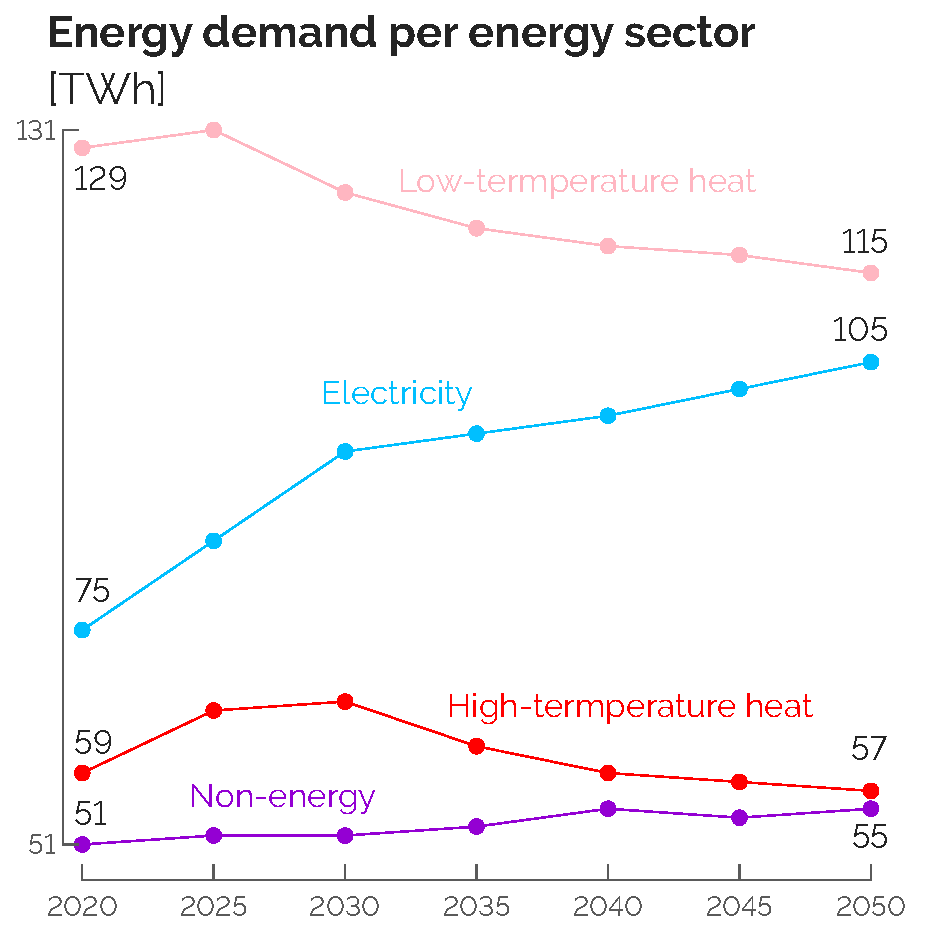
\includegraphics[width=0.49\textwidth]{EUD_sec.pdf}
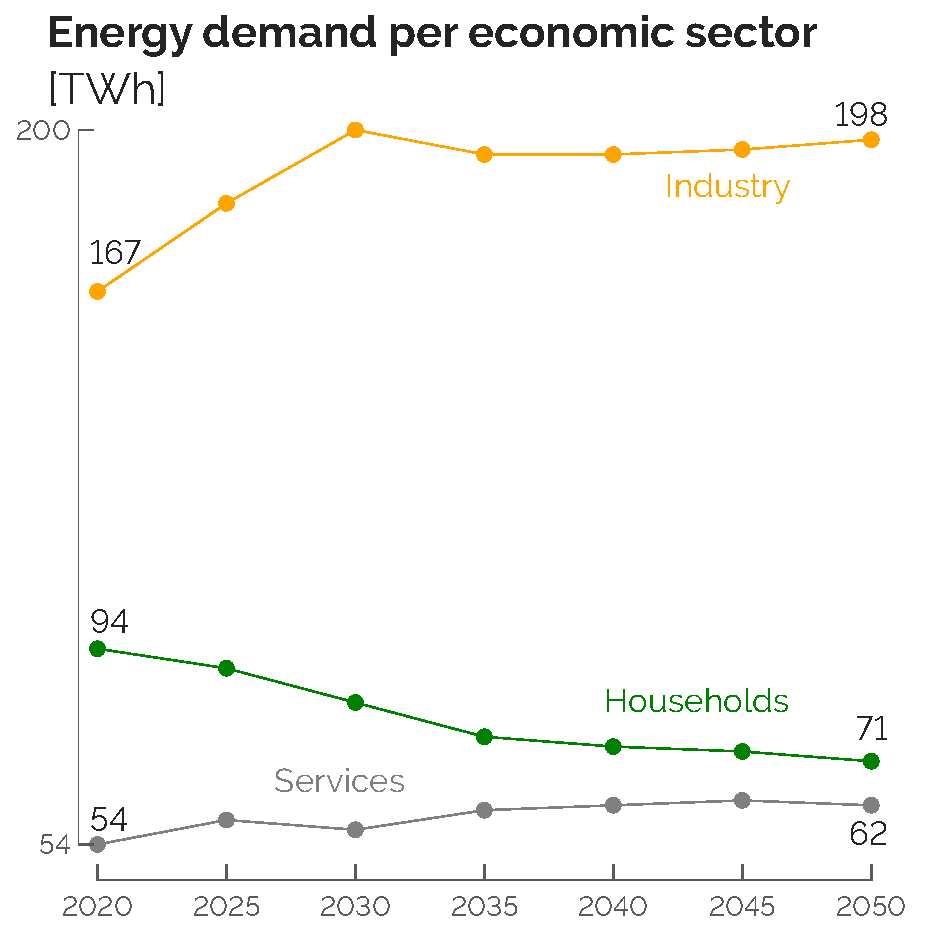
\includegraphics[width=0.49\textwidth]{EUD_cat.pdf}
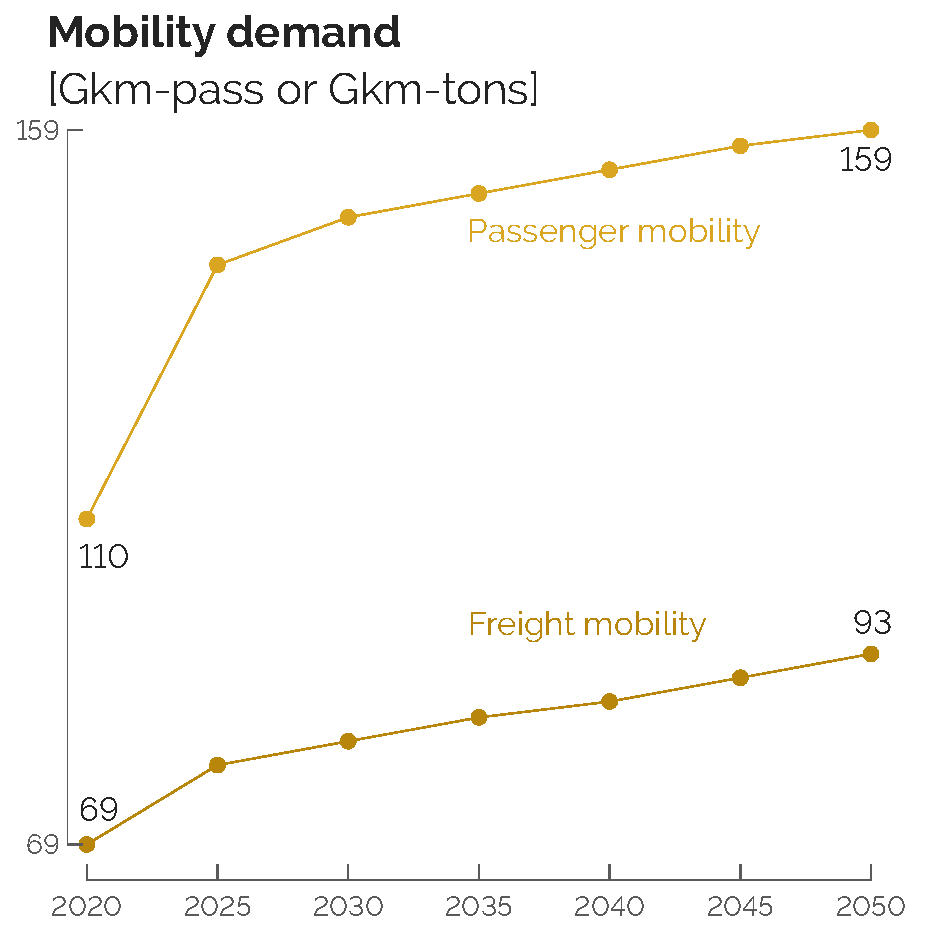
\includegraphics[width=0.49\textwidth]{EUD_mob.pdf}
\caption{EnergyScope splits the whole-energy system end-use demands (EUD) into two sets: (non)-energy and transport-related. This figure presents the nominal values of each of these demands. In the center graph, the non-energy demand has been fully associated with the industrial demand. As detailed previously, the non-energy demand is expressed in tons of physical products (\ie \glsxtrfull{HVC}, ammonia and methanol) and then translated into their respective energy equivalent, in TWh.}
\label{fig:cs_demands}
\end{figure}


\section{Resources}
\label{sec:cs:resources}
To supply the aforementioned demands, EnergyScope Pathway implements a variety of resources defined by their cost of purchasing, $\mathit{c}_{\mathrm{op}}$, their global warming potential, $\mathit{gwp}_{\mathrm{op}}$, as well as their 
availability, as detailed by \citet{limpens2024pathway}. First, the evolution of the respective costs of purchasing is presented (see \Cref{fig:cs_resources_cost}). Regarding ``renewable electrofuels'', these are in line with the recent study of \citet{genge2023supply} who carried out an extensive review and ``meta-analysis\cite{grant2009typology,page2021prisma} of 30 studies on the supply costs of chemical energy carriers''. Then, besides their cost, the resources are either limited or unlimited in terms of availability and either renewable or not. The limitation in terms of availability can be direct or indirect. On the one hand, woody (23.4\,TWh) and wet biomass (38.9\,TWh) are arbitrarily limited by their local potentials and the consumption of waste (17.8\,TWh) and coal (33.4\,TWh) is assumed not to exceed the current use. On the other hand, wind, solar, hydro and uranium are limited by the technical potentials of \gls{PV} panels (59.2\,GW), onshore (10\,GW) and offshore (6\,GW) wind turbines, run-of-the-river power plants (0.1\,GW) and nuclear power plants (6\,GW), respectively. In line with the work of \citet{PATHS2050} and the maximum capacity of conventional nuclear reactors that have been installed in Belgium, the same 6\,GW are assumed to be the maximum capacity for \gls{SMR}. Imported electricity is limited in two ways: the potential of instantaneous capacity of interconnection with neighbouring countries (\ie 11.9\,GW by 2050 \cite{ELIA_2050}) and a limitation to 30\% of the yearly electricity end-use demand (\ie 32.4\,TWh by 2050) \cite{limpens2021generating}. In the current work, the electrofuels (\ie e-methane, e-hydrogen, e-methanol and e-ammonia) are assumed to be ``sustainable" in the sense that they do not increase the concentration of \ce{CO2} in the atmosphere \cite{rixhon2021terminology}. In practice, it means that their \gls{GWP} is assumed to be zero in the model. Regarding specifically these electrofuels, the \citet{h2coalition} has carried out an extensive techno-economic analysis to estimate their respective cost of purchasing, after having identified some key locations from which importing these energy carriers (\eg Chile, Australia or Morocco). As the amount to import from each of these locations is hard to forecast, the current work considers the average cost between the different locations. Besides these, every other resource has its specific \gls{GWP} like coal ($\mathit{gwp}_{\mathrm{op,coal}}=0.40$\,kt$_{\ce{CO2},\text{eq}}$/GWh), natural gas ($\mathit{gwp}_{\mathrm{op,NG}}=0.27$\,kt$_{\ce{CO2},\text{eq}}$/GWh) or the fossil-based molecules equivalent to the electrofuels (\eg $\mathit{gwp}_{\mathrm{op,ammonia}}=0.46$\,kt$_{\ce{CO2},\text{eq}}$/GWh or $\mathit{gwp}_{\mathrm{op,methanol}}=0.41$\,kt$_{\ce{CO2},\text{eq}}$/GWh).

\begin{figure}[htbp!]
\centering

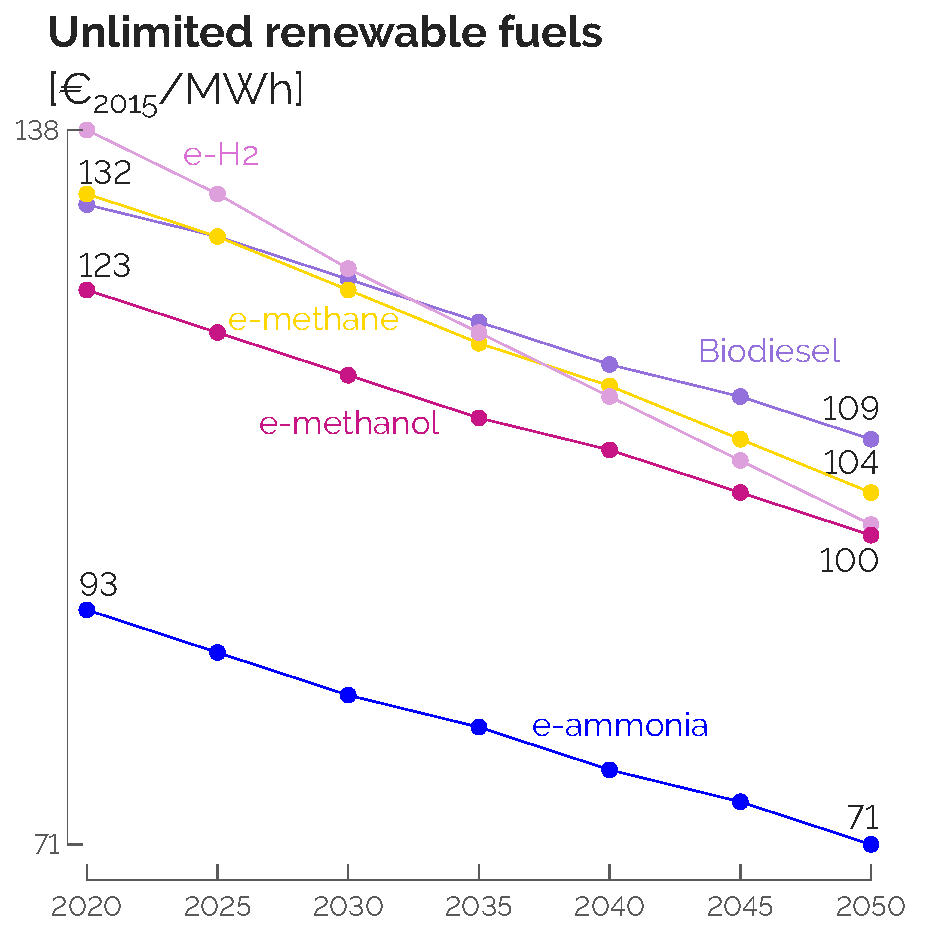
\includegraphics[width=0.49\textwidth]{Res_ren.pdf}
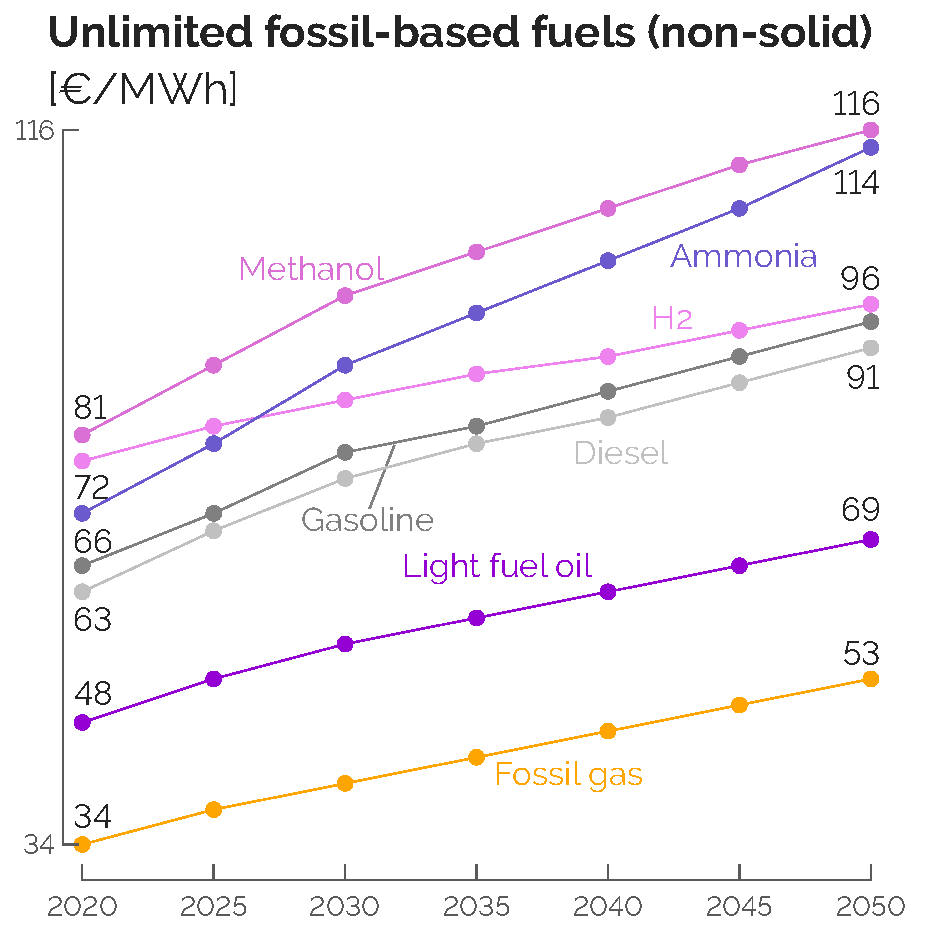
\includegraphics[width=0.49\textwidth]{Res_foss.pdf}
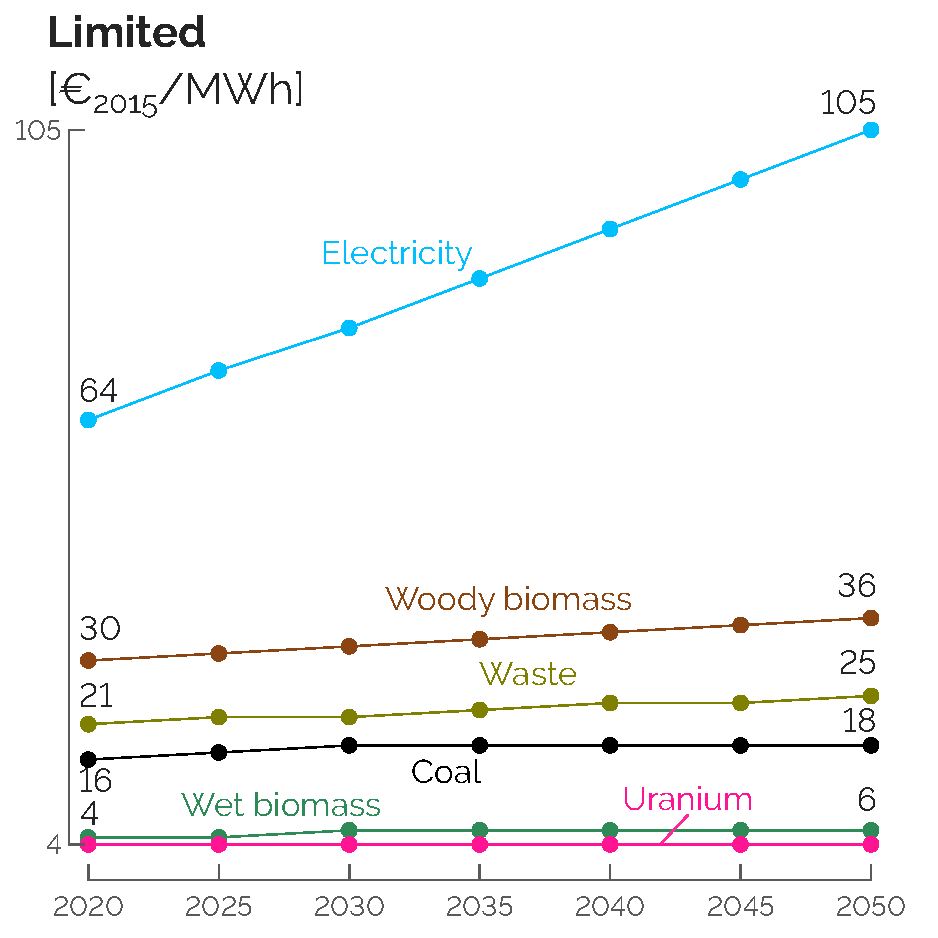
\includegraphics[width=0.49\textwidth]{Res_others.pdf}
\caption{Cost of purchasing the different resources. Besides the free local renewables (\ie sun, wind and hydro) limited by technical potentials, EnergyScope accounts for renewable energy carriers and their respective fossil counterparts (left and center graphs). These fuels can be imported from abroad without limitation on their availability. Other carriers are limited either by their local potentials (\ie biomass and waste) or other considerations like the power grid interconnections or the capacity of nuclear power plants.}
\label{fig:cs_resources_cost}
\end{figure}


\section{Conversion technologies}
\label{sec:cs:technologies}
As the end-use demands are defined as energy (and non-energy with the \gls{NED}) services rather than a certain quantity of oil or solar irradiance, for instance, technologies are implemented to convert these resources into the end-use demands. Besides their CAPEX, OPEX and lifetime defined in Section \ref{sec:meth:ES}, production and conversion technologies (\ie \gls{CCGT}, car or boiler) have a conversion efficiency whereas storage technologies (\ie thermal storage, battery or molecule storage) exhibit their own charge/discharge losses. There are also infrastructure technologies. They encompass, for instance, the power grid, the \gls{DHN} or technologies to produce intermediate energy carriers (\eg wood pyrolysis, biomethanolation or steam methane reforming to produce hydrogen). Not digging into too much details about the exhaustive list of these technologies presented in previous works \cite{limpens2021generating}, this section rather focuses on the implementation of \glsxtrfull{SMR} then the technologies to supply the \glsxtrfull{NED}.\\

\subsection{Small modular reactor}
\label{subsec:cs:SMR_tech}

A specific attention is to put on the implementation of \gls{SMR} whereas the 6\,GW of conventional nuclear are assumed to drop to 2\,GW in 2025 and total phase-out by 2035. Similarly to the analysis of \citet{PATHS2050}, a Belgian consortium for energy research, and in line with the Belgian Nuclear Research Centre (SCK-CEN) \cite{SCK-CEN_SMR}, \gls{SMR} are implemented with the features listed in \Cref{tab:SMR_features}. Where most of the features are similar to conventional nuclear power plants, it differs from these on two main points: their potential year start, 2040, and their flexibility. Indeed, unlike the current nuclear power plants, constrained in the model to produce a constant power output at every hour of the year (\ie baseload production as it is actually the case in Belgium), SMRs, are flexible in the sense that their production can vary between 0 and their full capacity independently at any hour of each representative year. Here, we simplify SMRs as only producing electricity and disregard the heat produced by the nuclear reaction. This is considered as lost to the atmosphere.

\begin{table}[htbp!]
\caption{Nominal features of the SMRs in EnergyScope. \gls{SMR} exhibits the advantage to have a fully flexible production (\ie between 0 to the full capacity) unlike conventional nuclear that is constrained to produce a constant baseload at every hour of the year.}
\label{tab:SMR_features}
\begin{minipage}{\linewidth}
\centering
\begin{tabular}{l c c}
\toprule
\textbf{Feature} & \textbf{Value} & \textbf{Unit}\\
\midrule
CAPEX & 4850 & €/kW \\
Annual OPEX & 103 & €/kW/year \\
Lifetime & 60 & year \\
Efficiency & 40\% & -\\
Maximum capacity & 6 & GW \\
Annual availability & 85\%\footnote{\label{foot:avail_SMR}This annual availability accounts for yearly maintenance where the reactors might not operate or, at least, not at their maximum capacity. } & -\\
Operational year & 2040\footnote{\label{foot:op_year_SMR}2040 is the soonest year at which \gls{SMR} could be available, optimistically assuming industrial prototypes being completed by 2035 and 5 additional years for their commercial installation.} & - \\
Flexibility & Full & - \\
\bottomrule							

\end{tabular}
\end{minipage}
\end{table}


%\begin{table}[htbp!]
%\caption{Nominal features of the SMRs in EnergyScope. \gls{SMR} exhibits the advantage to have a fully flexible production (\ie between 0 to the full capacity) unlike conventional nuclear that is constrained to produce a constant baseload at every hour of the year.}
%\label{tab:SMR_features}
%\centering
%\begin{tabular}{l c c|c}
%\toprule
%\multirow{2}{*}{\textbf{Feature}} & \multirow{2}{*}{\textbf{Value}} & \multirow{2}{*}{\textbf{Unit}} & \textbf{Similarity with}\\
% & & & \textbf{conventional nuclear}\\
%\midrule
%CAPEX & 4850 & €/kW & \checkmark\\
%Annual OPEX & 103 & €/kW/year & \checkmark\\
%Lifetime & 60 & year & \checkmark\\
%Efficiency & 40\% & -& \checkmark\\
%Maximum capacity & 6 & GW & \checkmark\\
%Annual availability & 85\%\footnote{\label{foot:avail_SMR}This annual availability accounts for yearly maintenance where the reactors might not operate or, at least, not at their maximum capacity. } & -& \checkmark\\
%\midrule
%Operational year & 2040\footnote{\label{foot:op_year_SMR}2040 is the soonest year at which \gls{SMR} could be available, optimistically assuming industrial prototypes being completed by 2035 and 5 additional years for their commercial installation.} & - & \xmark\\
%Flexibility & Full & - & \xmark\\
%\bottomrule							
%
%\end{tabular}
%\end{table}

For the sake of comparison, the \gls{LCOE} of the principal technologies to produce electricity, based on the computation used by \citet{limpens2021generating}, are detailed (see \Cref{fig:LCOE}). Not including here the cost of integrating a technology in the system (\eg reinforcement of the grid and storage capacities for \gls{VRES}), the \gls{LCOE} aims at aggregating and normalizing the CAPEX and OPEX of technologies providing a common commodity, \ie electricity. Compared to the other flexible generation units (\ie \gls{CCGT}), \gls{SMR} is significantly more cost-effective. Besides being about six times more capital-intensive in €/kW, the investment is amortized over a longer expected lifetime (\ie 60 years versus 25 for \gls{CCGT}). Moreover, the cost of purchasing uranium driving \gls{SMR} is expected to remain stable and low whereas the expected increase of the cost of purchasing fossil fuels dominates the \gls{LCOE} of \gls{CCGT}. In addition, one sees that \gls{CCGT} supplied by e-ammonia outcompetes its e-methane equivalent, unlike their respective fossil-based equivalent. This due to the fact that e-ammonia, not requiring carbon capture, is expected to be more cost-effective to produce versus e-methane \cite{h2coalition}. On the contrary, fossil-based ammonia, mostly relying on steam methane reforming, requires additional steps in the production process compared to fossil gas, as introduced in Section \ref{subsec:cs:NED}.

\begin{figure}[htbp!]
\centering
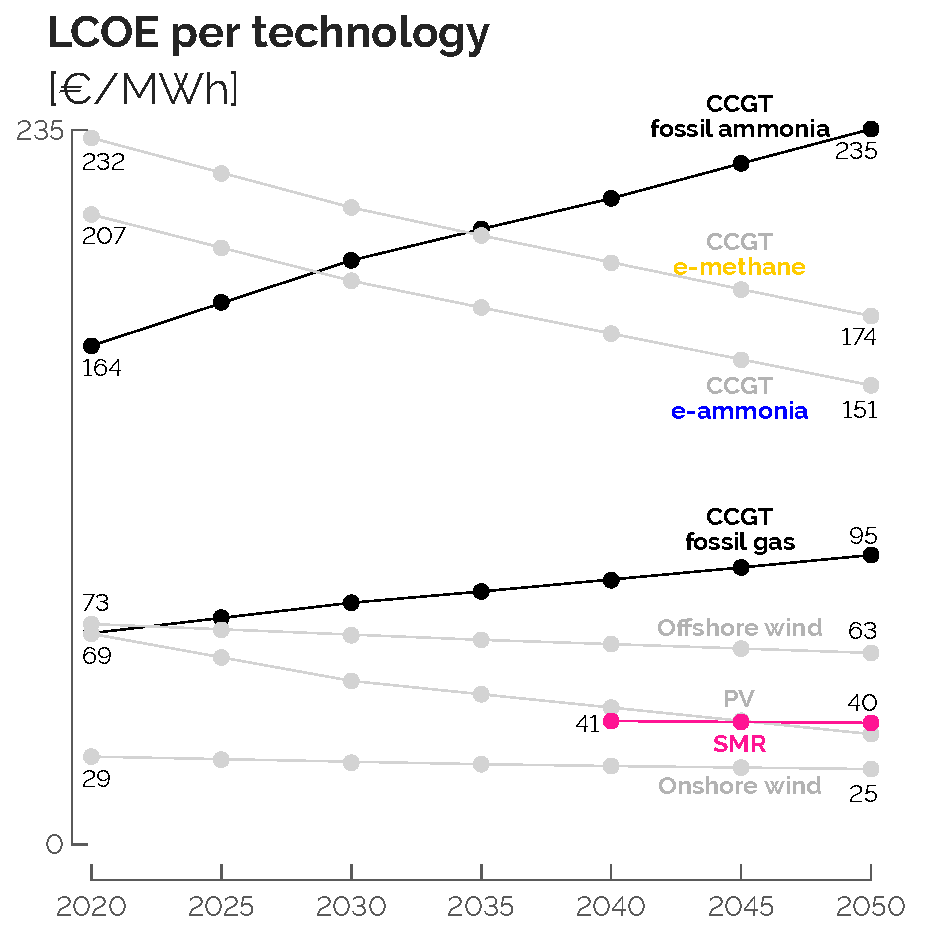
\includegraphics[width=0.49\textwidth]{LCOE_line_2.pdf}
\caption{Levelised cost of energy (LCOE) for the main technologies in the power sector. Gray and black curves are related to technologies runnning on renewable and fossil resources, respectively. Where \gls{SMR} is cheaper than the other flexible options, \gls{CCGT} running on e-ammonia is, a priori, cheaper than its e-methane alternative.}
\label{fig:LCOE}
\end{figure}

\subsection{Technologies supplying the non-energy demand}
\label{subsec:cs:NED_tech}

Different paths are implemented to produce the final molecules of the NED (see \Cref{fig:NED_tech}). Similarly to \citet{tsiropoulos2018emerging}, naphtha, here considered as \gls{LFO}, resulting from refinery operation is modeled as an imported commodity. Presented here for the specific year of 2035, all data and related references can be found in \cite{GIT_NED}. To keep the same level of details with other sectors of the model, the implementation of the conversion technologies consists of a single kind of technology per type of resource to produce a certain product. For instance, in the model, there is only one technology to produce \gls{HVC} either from naphtha or from LPG, two liquid fossil hydrocarbons, \ie \gls{NSC}. For ammonia and methanol, the molecules can either be produced locally from other resources or directly imported (with distinction between non-renewable and renewable molecules). 

\begin{figure}[htbp!]
\centering
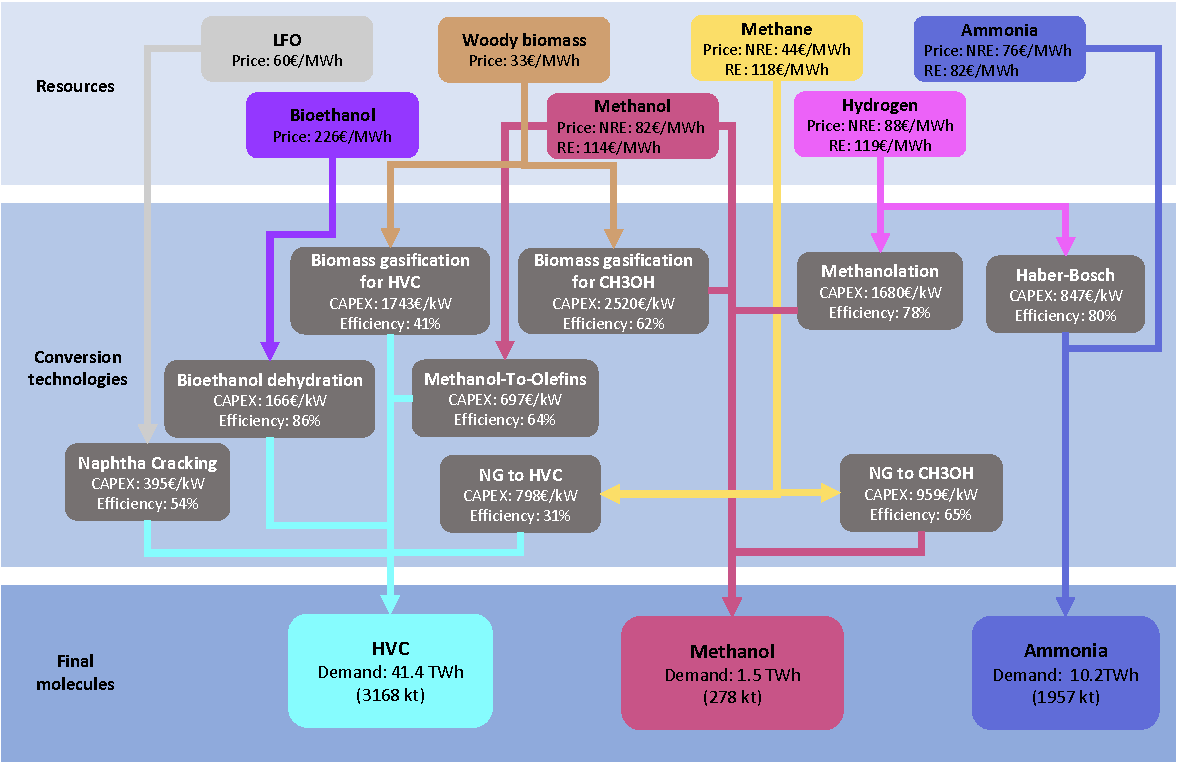
\includegraphics[width=0.8\textwidth]{NED_tech.pdf}
\caption{Schematic view of the different resources able to produce \gls{HVC}, ammonia and methanol with their related conversion technologies (including energy efficiency and their CAPEX - in €/kW of final molecules).  Values stand for 2035. Graph from \cite{rixhon2021comprehensive}}
\label{fig:NED_tech}
\end{figure}

\myparagraph{The impact of integrating the \gls{NED} in the Belgian whole-energy system}\\

\noindent
Works of \citet{rixhon2021comprehensive,rixhon2022integration} assessed the impact of the integration of the \gls{NED} in the case of Belgium, using EnergyScope TD (see Appendix \ref{app:ESTD}).  This snapshot model, \ie optimising the system in a target future year (\ie 2050 in this case) considering a green field approach, investigated the defossilisation of the system. To analyse the whole-energy system at different ``climate targets'', the model forced the total emissions to decrease by reducing their upper limit while optimising the total cost. In practice, 10\% steps of \gls{GWP} reduction were made from the ``reference scenario - 100\%''. This strategy gave the following points of analysis: 100\% (\ie cost-optimum with no limitation on the total \gls{GWP}), 90\%, 80\%, ..., down to 0\% (\ie  carbon-neutrality).\\

First and foremost, when the \gls{NED} is implemented with this higher level of details, we highlighted that woody biomass was ``cannibalised'' to produce methanol, instead of high-temperature heat, in the cost-optimum situation. At more ambitious ``climate targets'', e-methanol rises as the keystone to defossilise the \gls{NED} sector as \gls{MTO} becomes the favoured option to produce \gls{HVC}, representing the major share of the \gls{NED}. Then, including the \gls{NED} affects the selection of the technologies for the satisfaction of the heat and the electricity demands. The additional high-temperature demand required by the \gls{NED} forces the system to invest in more efficient technologies like \gls{CHP} instead of \gls{CCGT}. This additional heat demand mostly supplies naphtha-cracking substituted by \gls{MTO} at more ambitious ``climate targets'' to produce \gls{HVC}. To a lesser extent, to respect the emissions-caps, integrating the \gls{NED} leads to a higher integration of solar-\gls{PV} to support the electrification of the low-temperature heat sector.\\


For further details on these analyses, the interested reader is invited to refer to aforementioned for further published works.

\section{Uncertainty ranges}
\label{sec:cs:uncertainty}
As detailed in Section \ref{sec:meth:UQ}, accounting for uncertainty in \gls{ESOMs} is crucial \cite{mavromatidis2018uncertainty}, especially when it comes to optimise several decades in an inherently uncertain future. The fundamental step in this ambition is to characterise these uncertainties. In this work, following the approach of \citet{Moret2017PhDThesis}, we have defined range of uncertainties for the model parameters. \Cref{tab:UC_short} gives the uncertainty ranges of some key parameters. Like other works \cite{li2019renewables,coppitters2021robust}, the uncertain parameters are assumed to be independent and uniformly distributed between their respective lower and upper bounds. A particular attention is to pay to the potential installation of \gls{SMR}, at the bottom of \Cref{tab:UC_short}. As detailed before, the commercial availability of such a technology is uncertain but would not be before 2040. Consequently, for \gls{SMR}, the parameter $f_{\mathrm{max,SMR}}$ influences the maximum capacity to install to translate somehow the readiness of this technology. Arbitrarily, we have then assumed the following probability of availability of such a technology: 10\% of chance to be installable from 2040, 20\% from 2045 and 40\% from 2050\footnote{In other words, if this parameter, ranging between 0 and 1, is (i) smaller than 0.6, there is no possibility to install \gls{SMR} during the transition; (ii) between 0.6 and 0.8, these 6~GW can be installed only in 2050; (iii) between 0.8 and 0.9, these can be installed from 2045 onward and; (iv) higher than 0.9, the prescribed maximum capacity can be installed from 2040 onward. }. Based on the local sensitivity analysis carried out by \citet{PATHS2050}, the current work also considers a [-40\%; +44\%] range on the CAPEX of SMR, on top of the uncertainty about the availability. Finally, the the cost of purchasing renewable electrofuels presents a wide range, [-64.3\%; +179.8\%], like the other imported commodities.

The exhaustive list of the parameters accounted in this work is presented in Appendix \ref{app:UC_full}.

\begin{table}[htbp!]
\caption{Illustration of the uncertainty characterisation for different parameters for the year 2025. }
\label{tab:UC_short}
\begin{minipage}{\linewidth}
\centering
\resizebox{\textwidth}{!}{
\begin{tabular}{l l l c c c}
\toprule
\multirow{2}{*}{\textbf{Category}} & \multirow{2}{*}{\textbf{Parameter}} & \multirow{2}{*}{\textbf{Meaning}} & \multirow{2}{*}{\textbf{Type}\footnote{\label{foot:type_uncert_range}Per \citet{Moret2017PhDThesis}, \og I: investment-type, II: operation-type (constant uncertainty over time), III: operation-type (uncertainty increasing over time)\fg. }}  & \multicolumn{2}{c}{\textbf{Relative variation\footnote{\label{foot:nom_val_uncert}The nominal values of each of the parameters is 0, meaning no variation compared to the nominal values of the impacted parameter in the model. }}}\\
    & & & &	 min 	&	 max \\ 	
\midrule		
\multirow{2}{*}{\textbf{Cost of purchasing}} & $c_{\mathrm{op,fossil}}$ & Purchase fossil fuels & II & -64.3\% & 179.8\% \\
& $c_{\mathrm{op,electrofuels}}$ & Purchase electrofuels & II & -64.3\% & 179.8\% \\
\midrule
\multirow{5}{*}{\textbf{Investment cost}} &$c_{\mathrm{inv,car}}$ & CAPEX car  & I & -21.6\% & 25.0\% \\
& $c_{\mathrm{inv,e\_prop}}$ & CAPEX electric motor & I & -39.6\% & 39.6\% \\
& $c_{\mathrm{inv,fc\_prop}}$ & CAPEX fuel cell engine & I & -39.6\% & 39.6\% \\
& $c_{\mathrm{inv,PV}}$ & CAPEX PV & I & -39.6\% & 39.6\% \\
& $c_{\mathrm{inv,nuclear\_SMR}}$ & CAPEX \gls{SMR}\footnote{\label{foot:range_SMR}This range has been inferred from the local sensitivity analysis performed by \citet{PATHS2050}.}& I & -40.0\% & 44.0\% \\
\midrule
\multirow{1}{*}{\textbf{Consumption}} &$\eta_{\mathrm{e\_prop}}$ & Consumption electric vehicles & I & -28.7\% & 28.7\% \\
\midrule
\multirow{2}{*}{\textbf{Potential installed capacity}} &$f_{\mathrm{max,PV}}$ & Max capacity PV & I & -24.1\% & 24.1\% \\
& $f_{\mathrm{max,windon}}$ & Max capacity onshore wind & I & -24.1\% & 24.1\% \\
\midrule
\multirow{2}{*}{\textbf{Hourly load factor}} & $c_{\mathrm{p,t,PV}}$ & Hourly load factor PV & II & -22.1\% & 22.1\% \\
& $c_{\mathrm{p,t,winds}}$ & Hourly load factor wind turbines & II & -22.1\% & 22.1\% \\
\midrule
\multirow{2}{*}{\textbf{Resource availability}} & $avail_{\mathrm{elec}}$ & Available electricity import & I & -32.1\% & 32.1\% \\
& $avail_{\mathrm{biomass}}$ & Available local biomass & I & -32.1\% & 32.1\% \\
\midrule

\multirow{2}{*}{\textbf{End-use demand}} & $pass\_EUD$ & Passenger mobility EUD & III & -7.5\% & 7.5\% \\
& $industry\_EUD$ & Industry EUD & III & -20.5\% & 16.0\% \\
\midrule

\multirow{4}{*}{\textbf{Miscellaneous}} &$i_{\mathrm{rate}}$  & Interest rate & I & -46.2\% & 46.2\% \\
& $\Delta_{\mathrm{change,freight}}$ & Modal share change freight mobility & - & -30\% & 30\% \\
& $\Delta_{\mathrm{change,pass}}$ & Modal share change passenger mobility & - & -30\% & 30\% \\
& $f_{\mathrm{max,SMR}}$ & Potential capacity \gls{SMR} & - & 0 & 1 \\

\bottomrule							

\end{tabular}}
\end{minipage}
\end{table}

\section{\ce{CO2}-budget for the transition}
\label{sec:cs:CO2-budget}
In most of the studies carried out on the pathway optimisation of a whole-energy system, a \ce{CO2}-trajectory is \textit{a priori} set to reach carbon-neutrality by 2050. \citet{nerini2017myopic} used the emission trajectory indicated by the UK's Committee on Climate Change in their analysis of the impact of limited foresight to achieve the target of 80\% reduction of \gls{GHG} by 2050 in the United Kingdom. In their assessment of the impacts of economy-wide emissions policies in the water-energy-land nexus, \citet{licandeo2023assessing} analysed different \ce{CO2}-trajectories considering more or less severe water scarcity for the US. \citet{poncelet2016myopic} with LUSYM (Leuven University SYstem Model) and \citet{PATHS2050} with TIMES-BE also set decreasing emission trajectories in their analysis of respectively the Belgian power sector and whole-energy system.  Others only set the objective as the carbon-neutrality by 2050. For instance, \citet{heuberger2018impact} investigated the impact of different factors (\eg limit of the foresight in the future, availability of \og unicorn technologies\fg or committed versus market-driven decarbonisation strategies) to reach this ultimate objective in the UK system.\\

In this work, the effect of greenhouse gases is cumulative over time and a constraint is set on the overall emissions of the transition---a \ce{CO2}-budget for the transition. This approach is in line with the works defining safe operating spaces within the nine different global planetary boundaries (\ie (i) novel entities, (ii) stratospheric ozone depletion, (iii) atmospheric aerosol loading, (iv) ocean acidification, (v) biogeochemical flows, (vi) fresh water change, (vii) land system change, (viii) biosphere integrity, and, (ix) climate change) \cite{richardson2023earth,steffen2015planetary,rockstrom2009safe}. This ``systemic framework for addressing global anthropogenic impacts on Earth system'' gives quantitative recommendations about the \ce{CO2} concentration, among others, to maintain ``the stability and resilience of Earth system as a whole'' \cite{richardson2023earth}. In their review, \citet{ryberg2020downscaling} identified three main sharing principle categories when considering these safe spaces: \ie \textit{utilitarian}, \textit{egalitarian} and \textit{acquired rights} principles.In a nutshell, the former, mostly applied to the scale of industry sector \cite{ryberg2018bring,brejnrod2017absolute}, aims at maximising the sum of welfare. The second shares the so-called ``budget'' equally among the total population, allocating the same share to each individual \cite{hoff2017bringing,o2018good}. Finally, in \textit{acquired rights} principles, also called ``grandfathering'', the sharing is based on \og maintaining that prior emissions increase future emission entitlements\fg  \cite{knight2013grandfathering}.In this thesis, we have chosen the latter principle to allocate the \ce{CO2}-budget to the Belgian transition. This budget (1.2\,Gt$_{\ce{CO2},\text{eq}}$) corresponds to the proportion of Belgium's emissions in the world emissions in 2020 (34.8\,Gt$_{\ce{CO2},\text{eq}}$ \cite{ourworldindata_CO2_world}) applied to the global budget to have a 66\% chance of limiting warming to 1.5°C of 420\,Gt$_{\ce{CO2},\text{eq}}$ \cite{IPCC_CO2_budget}. Therefore, in this work, a limit has been put on $\emph{gwp\textsubscript{lim,trans}}=1.2\,\text{Gt}_{\ce{CO2},\text{eq}}$ in Eq.\,(\ref{eq:limit_gwp_trans}). This is another sign of the urgency to act to mitigate climate change as this 30-year budget represents only 10 years of the current emissions. \\

Compared to a linear decrease from the current emissions, as done by \citet{limpens2024pathway}, this budget represents a 60\% reduction of the cumulative emissions over the transition.  Appendix \ref{app:CO2_budget} compares the emissions trajectory between the REF case and a case (without \gls{SMR}) where the linear decrease is imposed between 2020 and carbon-neutrality in 2050.
\clearpage

%% -- Chapter 4 - Atom vs. molecule -----------------------------
\clearemptydoublepage
\chapter{The atom-molecules dilemma: deterministic and uncertain analyses} 
\label{chap:atom_mol}
%!TEX root = ../thesis_main.tex
%!TEX encoding = UTF-8 Unicode
\vspace{-0.2cm}
\begin{flushright}
\emph{``It is difficult to make predictions, especially about the future.''}\\
Niels Bohr, in \textit{Bulletin of the Atomic Scientists}, 1971
\end{flushright}
\vspace{0.4cm}

On top of scenarios with more profound behavioural changes, variety of technological pathways are often investigated to meet the ambitions of climate change mitigation. For instance, in their work, \citet{My2050} assessed different scenarios for a climate neutral Belgium by 2050. Depending on the scenarios, the emphasis is put on a higher electrification of the whole-energy system, a higher consumption of hydrogen or more complex moleclules (\ie electrofuels) or a bigger reliance on biomass and the related \gls{BECCS}. Besides these, ``unicorn'' technologies are also investigated \cite{heuberger2018impact}. These technologies have not (yet) reached a high enough maturity, \ie Technology Readiness Level (TRL) 3 to 7, or they face hurdles such as social acceptance. Therefore, they are currently not deployed on a large scale. Among others, nuclear energy finds an interest in the literature \cite{IEA_Nuclear_2022,PATHS2050}. In the form of \acrfull{SMR}, nuclear energy is also discussed in actual current investments (in Belgium for instance \cite{SMRlesoir}).

In the future, deeper integration of \gls{VRES} will come with the bigger electrification of sectors like mobility, low-temperature and industry \cite{IEA2023electrification}. In such a context, there is a case for nuclear energy to produce a reliable low-\ce{CO2}emission electricity \cite{IAEA2008}. This is also in line with the willingness to phase out of imported Russian fossil fuels anchored in the European REPowerEU Plan \cite{REPowerEU}. Unlike the consumption of fossil gas that represents about 80\% of the \gls{LCOE} from \gls{CCGT}, the price of uranium accounts for 25-30\% of \gls{LCOE} from nuclear power plants. This favours nuclear energy against price volatility and for the security of electricity supply, in case of a conflict like the invasion of Ukraine, for instance.

In a country like Belgium, reaching the goal of energy transition will not be a ``winner-takes-all'' situation but rather a combination of solutions \cite{Limpens2020,limpens2021generating}. However, this chapter focuses on this atom-molecules dilemma. Often compared, if not opposed, to local renewables like wind and solar \cite{suna2016nuclear,khatib2016economics}, this chapter rather assesses the integration of nuclear energy in the future versus the need to import renewable molecules from abroad, in a country where the local potential of \gls{VRES} is limited compared to its \gls{EUD}. 

Section \ref{sec:atom_mol:results_deter} targets the impact of integrating \gls{SMR} from 2040 onward on the whole-energy system, in a deterministic way (\ie considering only nominal values of the parameters). 

In their review, \citet{yue2018review} pointed out that uncertainties were accounted for either snapshot models (\ie optimizing a single target future year), to assess a single energy sector (\ie the power sector, most of the time) or with limited number of uncertain parameters, \ie about ten, in a stochastic programming approach to optimize a transition pathway with a small number of time stages, \ie two or three. Here, the uncertainty quantification addresses the total transition pathway of the whole-energy system, with 34 uncertain parameters (see Appendix \ref{app:UC_full}). Accounting for uncertainties presented in Section \ref{sec:meth:UQ}, Section \ref{sec:atom_mol:results_uq} will identify the key factors driving higher or lower imports of electrofuels as well as the installation of \gls{SMR}, by the end of the transition, \ie 2050.

Relying on nuclear energy for some is highly controversial. On top of purely techno-economic aspects, non-exhaustively mentioned beforehand, there are other ethical, societal or even political considerations to account for when addressing this question \cite{kempf2022}. In the same sense, on top of ethical or geopolitical aspects, one could question the availability of the imported electrofuels, assumed to be unlimited in this work (see Chapter \ref{chap:case_study}). In their work, \citet{lefebvre2022electrofuel} investigated this topic for the case of Belgium considering lower and upper bounds in terms of availability based on, on the one hand, the already signed agreements with the exporting countries and, on the other hand, their maximal technological potential of \gls{VRES}, respectively. Their lower bound resulted in a total availability of electrofuels that is one order of magnitude lower than the needs provided by the cost-optimum carbon-neutral Belgium in 2050. Like the rest of this thesis, the purpose here is only to expose the impact of integrating \gls{SMR} as well as the need of importing electrofuels in the Belgian energy landscape, on a strictly techno-economical point of view with a cost-based optimisation. This is why, for the sake of transparency, the model and the data are documented and openly available online \cite{readthedocs_pathway} and in the Appendices \ref{app:EnergyScope} and \ref{app:case_study}.

\section{Deterministic impact of integrating \gls{SMR} in 2040}
\label{sec:atom_mol:results_deter} 
In this section, like in the rest of the thesis, the \textbf{REF} case is without any deployment of \gls{SMR} anytime during the transition and whereas in the \textbf{SMR} case this technology is available, up to 6\,GW (see Chapter \ref{chap:case_study}), from 2040 onward. After investigating the deployment of \gls{SMR} through the power sector, the first part of this section focuses on this impact on the whole-system level considerations (\ie overall transition costs, primary energy mix and yearly emissions per sector). The second part will address the impact of \gls{SMR} on each of the other sectors of the system.

\subsection{Power sector}
\label{subsec:atom_mol:results_deter_power_sector}
\gls{SMR} is deployed as soon as available, \ie 2040, to their maximum capacity, 6\,GW, substituting other flexible power generation units (see \Cref{fig:results_deter_tech_cap_elec}). There is no ammonia-\gls{CCGT} at the end of the transition and an anticipatory reduction of methane \gls{CCGT} (\ie 2.1\,GW in 2040 versus 3.7\,GW for the REF case). To a lesser extent, the last 2\% deployment of solar-\gls{PV} is slightly delayed as the capacity in 2025 is 1.3\,GW smaller than in the REF case. Overall, given the smaller efficiency of \gls{SMR}, \ie 40\% versus 51\% for ammonia-\gls{CCGT}, the restriction on yearly availability and the slightly higher electrification (\Cref{fig:results_deter_layer_elec}), the total power capacity installed by 2050 is 3.5\% higher for the SMR case. In their work, \citet{PATHS2050} also showed that \gls{SMR} first substitutes ``e-fuels/hydrogen'' turbines before reducing the need for \gls{PV}. However, in their ``Central'' scenario where no \gls{SMR} is installed by 2050, they rely on 96.6\,GW of \gls{PV}, 63\% more than the 59.2\,GW potential considered in our work and about 15 times more than the current installed capacity, \ie 6.5\,GW. \\

\begin{figure}[htbp!]
\centering
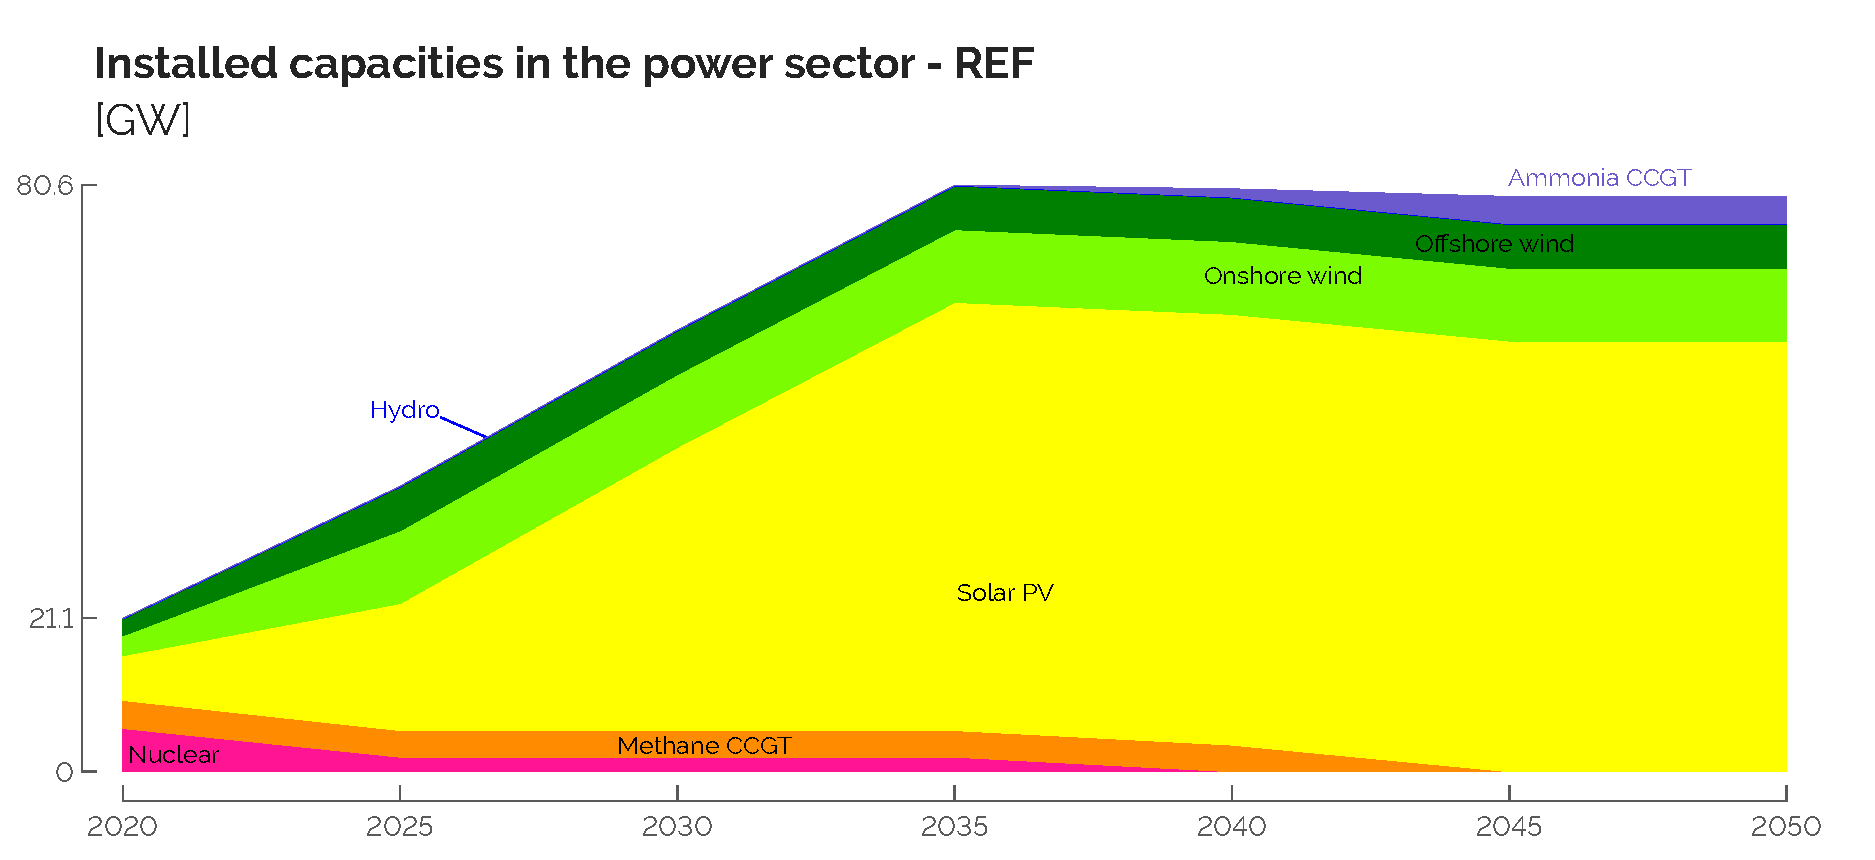
\includegraphics[width=0.8\textwidth]{Elec_Tech_Cap_REF.pdf}
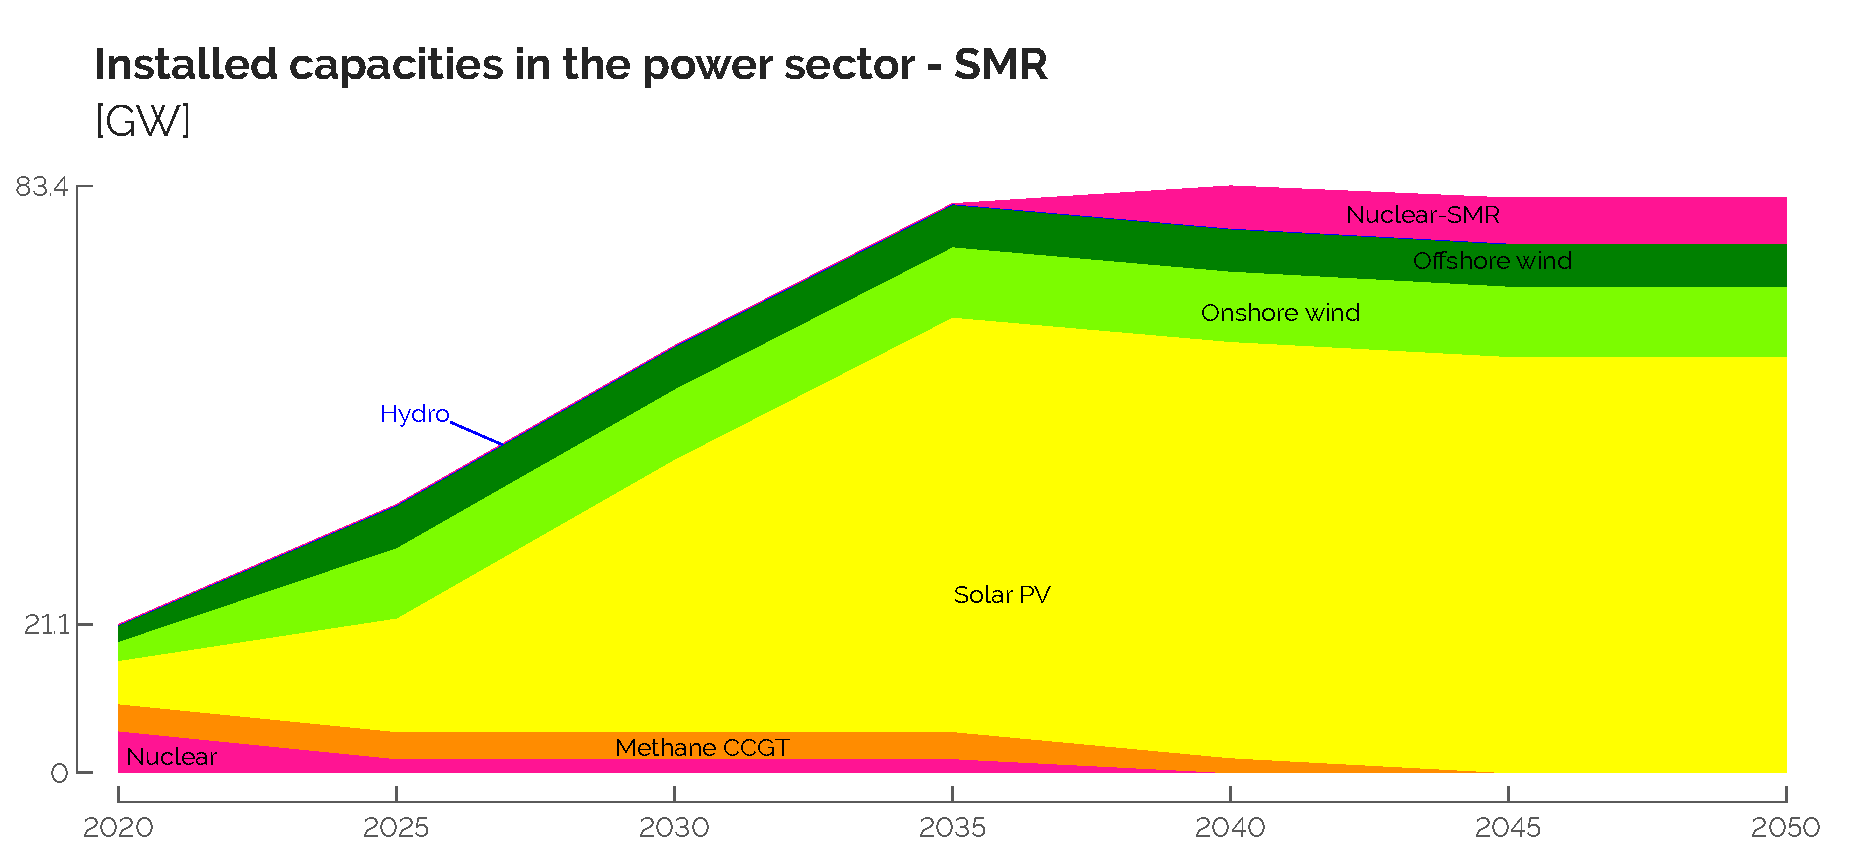
\includegraphics[width=0.8\textwidth]{Elec_Tech_Cap_SMR.pdf}
\caption{As soon as available (\ie 2040), \acrfull{SMR} is deployed to their maximum potential (\ie 6\,GW) to substitute more expensive flexible generation units (\ie gas and ammonia \gls{CCGT}).}
\label{fig:results_deter_tech_cap_elec}
\end{figure}

When assessing the electricity production-versus-consumption-balance (\Cref{fig:results_deter_layer_elec}), \gls{SMR}, as a cheaper, flexible and low-emitting power generation system, produces to its full capacity. Given the 15\% maintenance off-time assumed in this work, this represents 44.6\,TWh by 2050. In comparison, in 2020, conventional nuclear power plants produced 34.4\,TWh Belgium. This resurgence of nuclear electricity occurs at the expense of other, although more efficient, technologies: \gls{CCGT} and industrial \gls{CHP}. Besides the unchanged end-use-demand compared with the REF case, we observe a slight increase of the electrification of the rest of the system: +9.4\% which corresponds to +5.8\,TWh, mostly consumed by electric heaters in industry (+48\%) to produce industrial high-temperature heat.

\begin{figure}[htbp!]
\centering
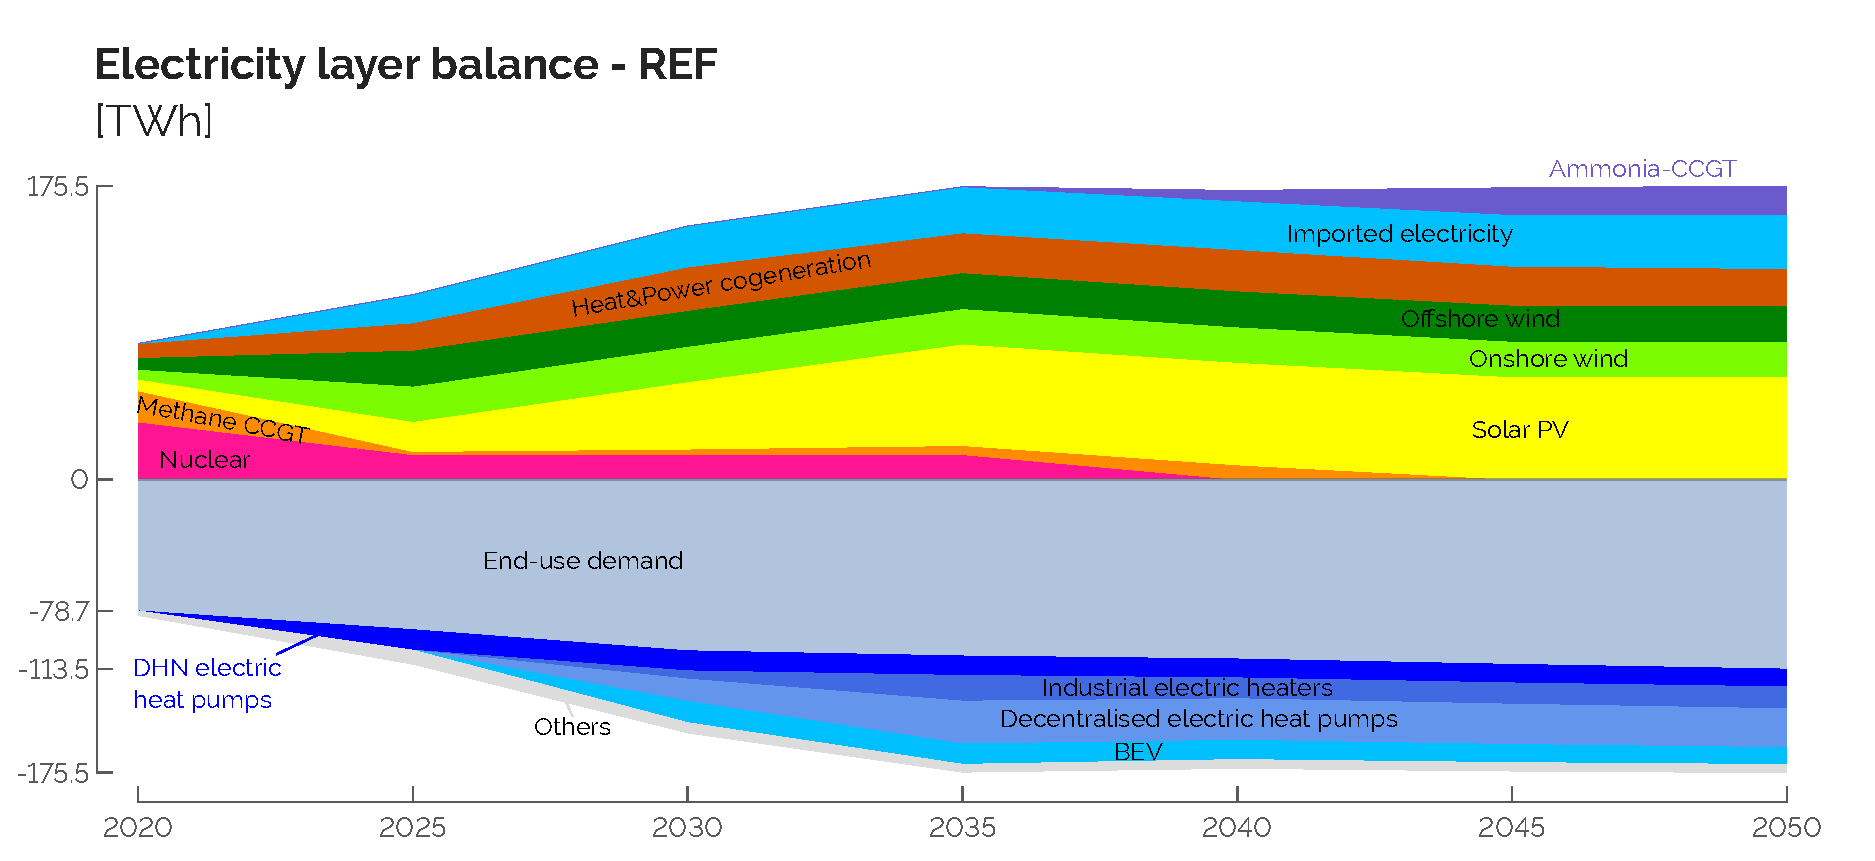
\includegraphics[width=0.8\textwidth]{Elec_Layer_REF.pdf}
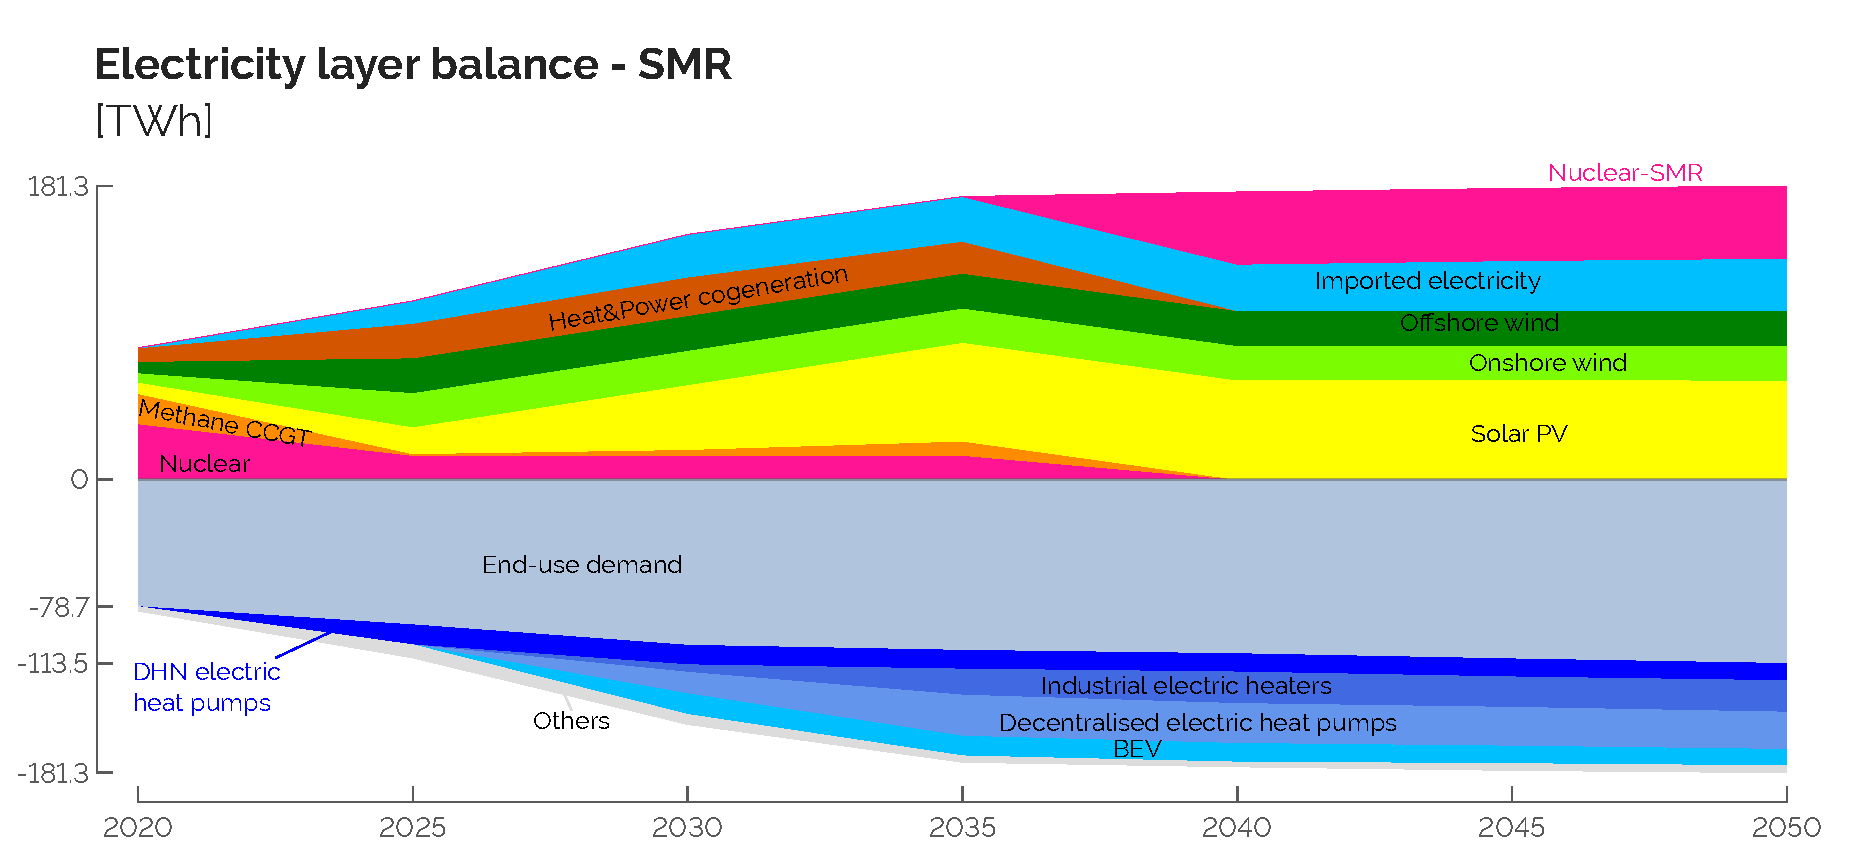
\includegraphics[width=0.8\textwidth]{Elec_Layer_SMR.pdf}
\caption{The production of electricity from \gls{SMR} substitutes more efficient technologies (\ie \gls{CCGT} and \gls{CHP}) and boosts the electrification of the rest of the system, mostly the industrial high-temperature heat sector.}
\label{fig:results_deter_layer_elec}
\end{figure}


\subsection{System-level impacts}
\label{subsec:atom_mol:results_deter_overall}
First of all, the 6\,GW \gls{SMR} installed from 2040 allow reaching a 3.3\% (-36.9\,b€) cheaper overall transition (\Cref{fig:results_deter_overall_emissions_sector}). Over the 30-year transition, this represents an annual cost saving equal to 0.2\% of the Belgian GDP. Thanks to the perfect foresight approach, the model knows ahead that cheaper and low-emitting \gls{SMR} will be available in the future. As the model can freely spend the constrained \ce{CO2}-budget over the transition, cost-savings also occur before 2040. These early-stage cost-savings are equally shared between the extended use of cheaper \gls{LFO} to produce \gls{HVC} and the delayed deployment of \gls{PV}. Then, the capital-intensive investments in \gls{SMR}, mostly recovered by the end of the transition as salvage value, are widely compensated by the smaller resource-related OPEX. This leads, at the end, aggregating the OPEX and the annualised CAPEX, to a system that is yearly 4.4\,b€ (8.8\%) cheaper by 2050 than in the REF case (Figure \ref{fig:results_deter_overall_emissions_sector}).

\begin{figure}[htbp!]
\centering
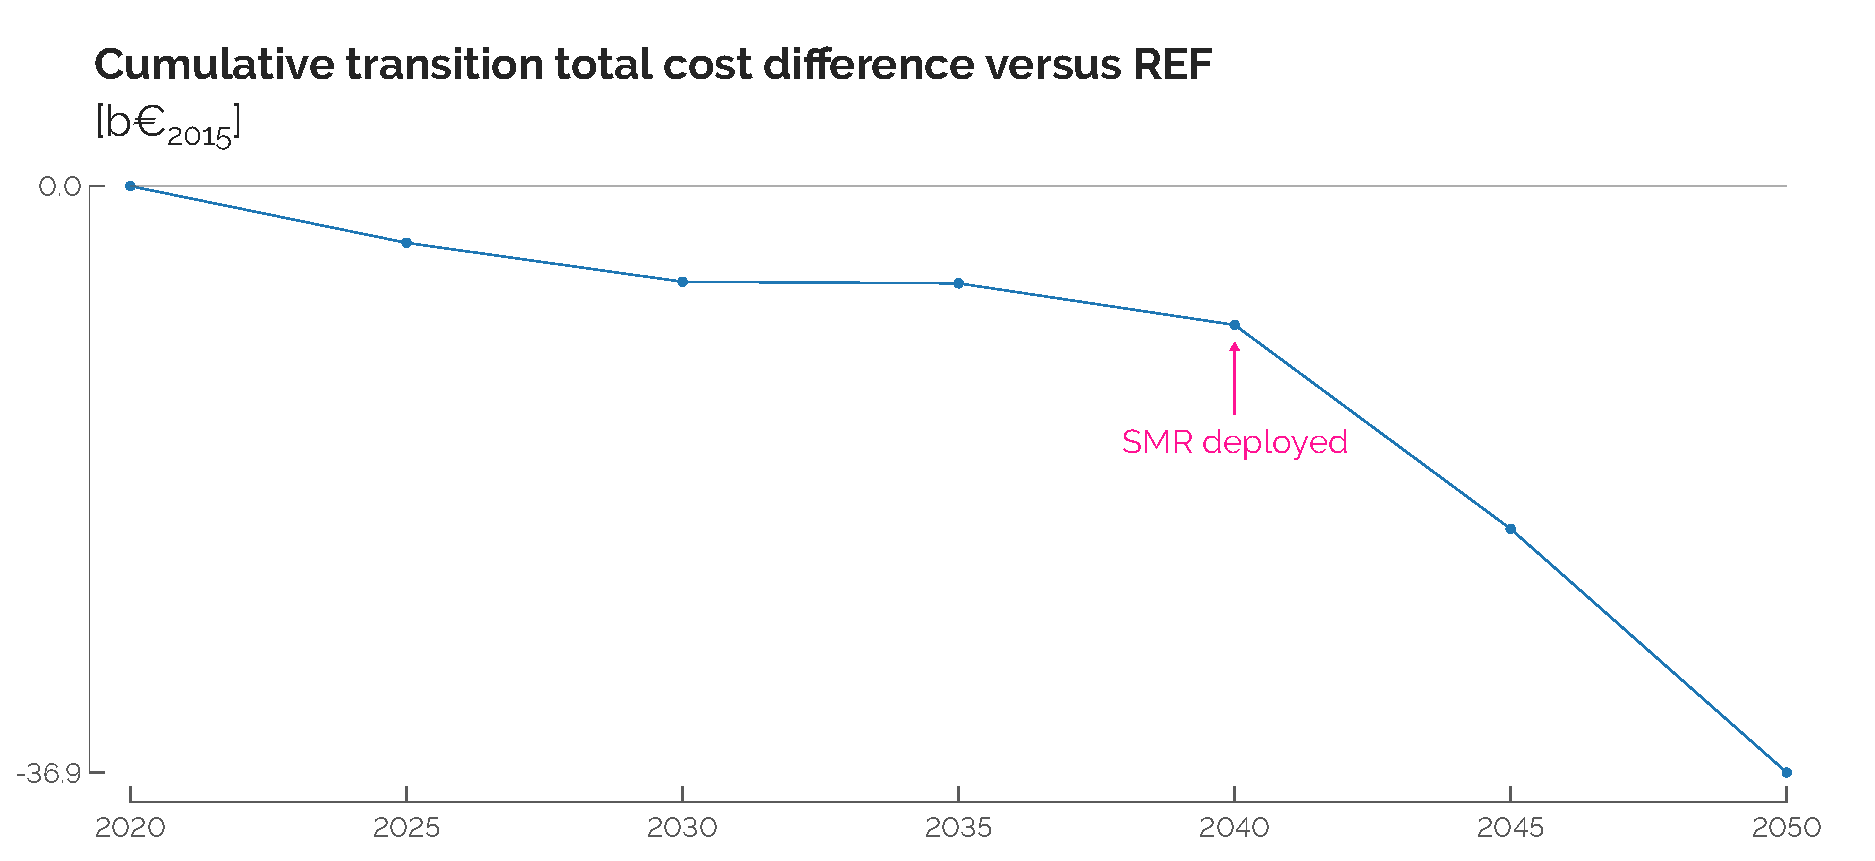
\includegraphics[width=0.8\textwidth]{Cum_total_cost_diff_REF.pdf}
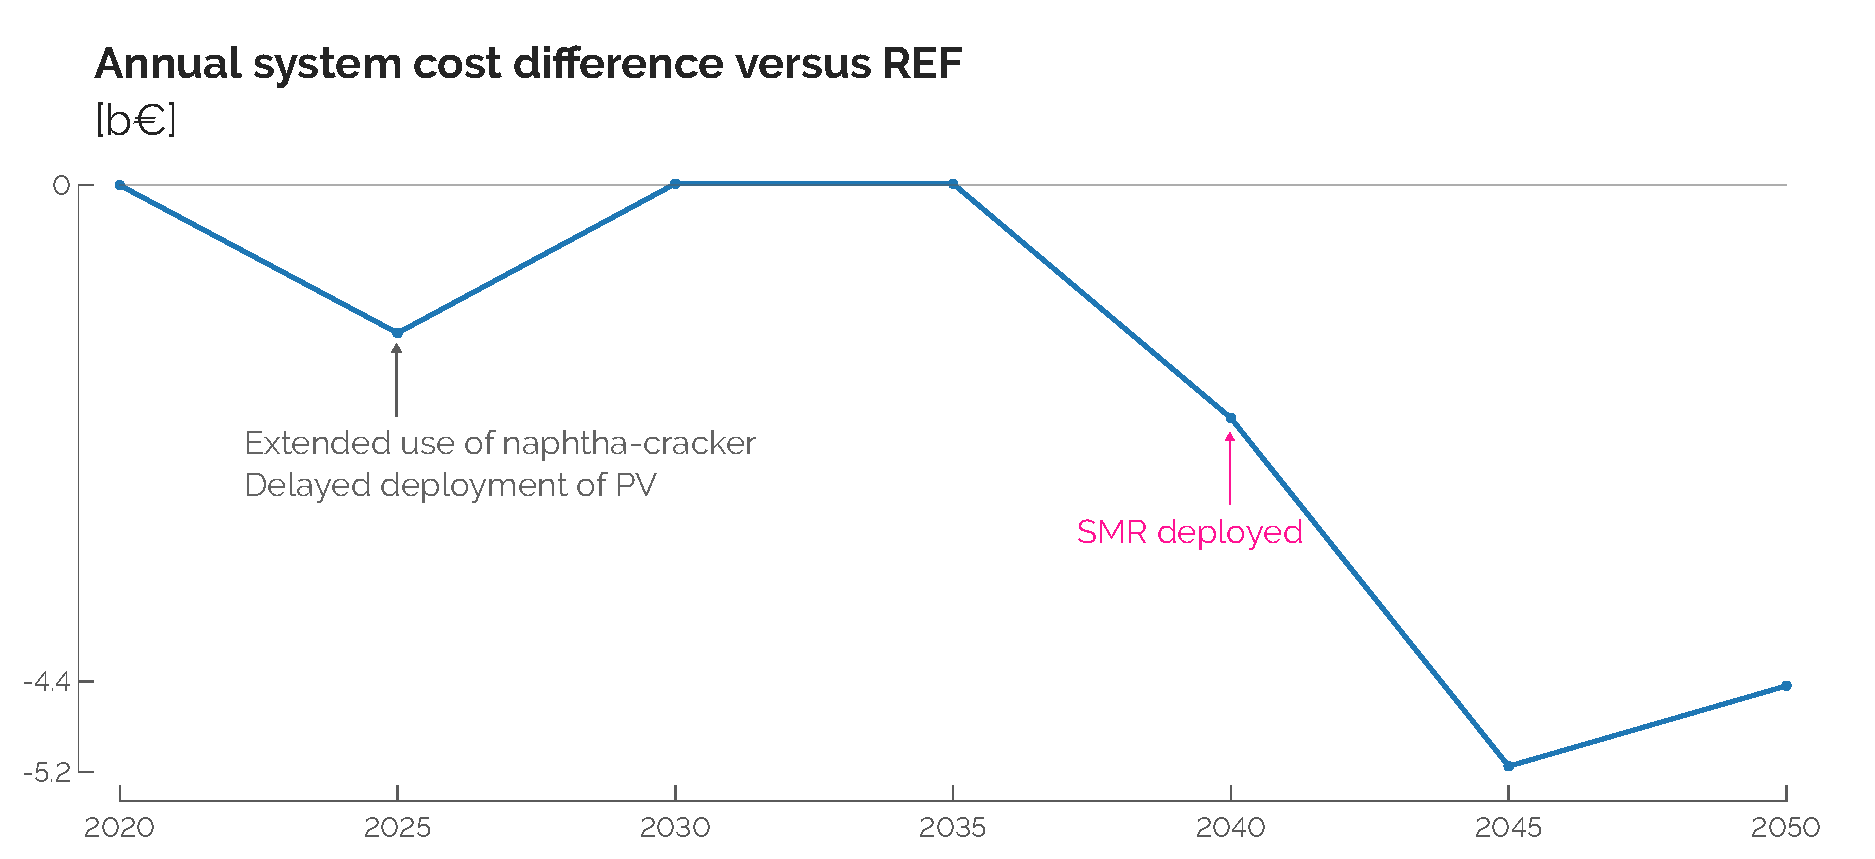
\includegraphics[width=0.8\textwidth]{System_cost_DIFF.pdf}
\caption{(Top) Cumulative transition cost and (down) annual system cost differences between the SMR and the REF cases. Including \gls{SMR} ends up in a cheaper overall transition (-36.9\,b€) and cheaper whole-energy system by 2050 (-4.4\,b€).}
\label{fig:results_deter_overall_emissions_sector}
\end{figure}

Extending the use of naphtha-cracker and, to a lesser extent the postponing the deployment of PV, lead to higher \ce{CO2}-emissions at the beginning of the transition that are then compensated by the deployment of \gls{SMR} (\Cref{fig:GWP_per_sector_diff}). 

\begin{figure}[htbp!]
\centering
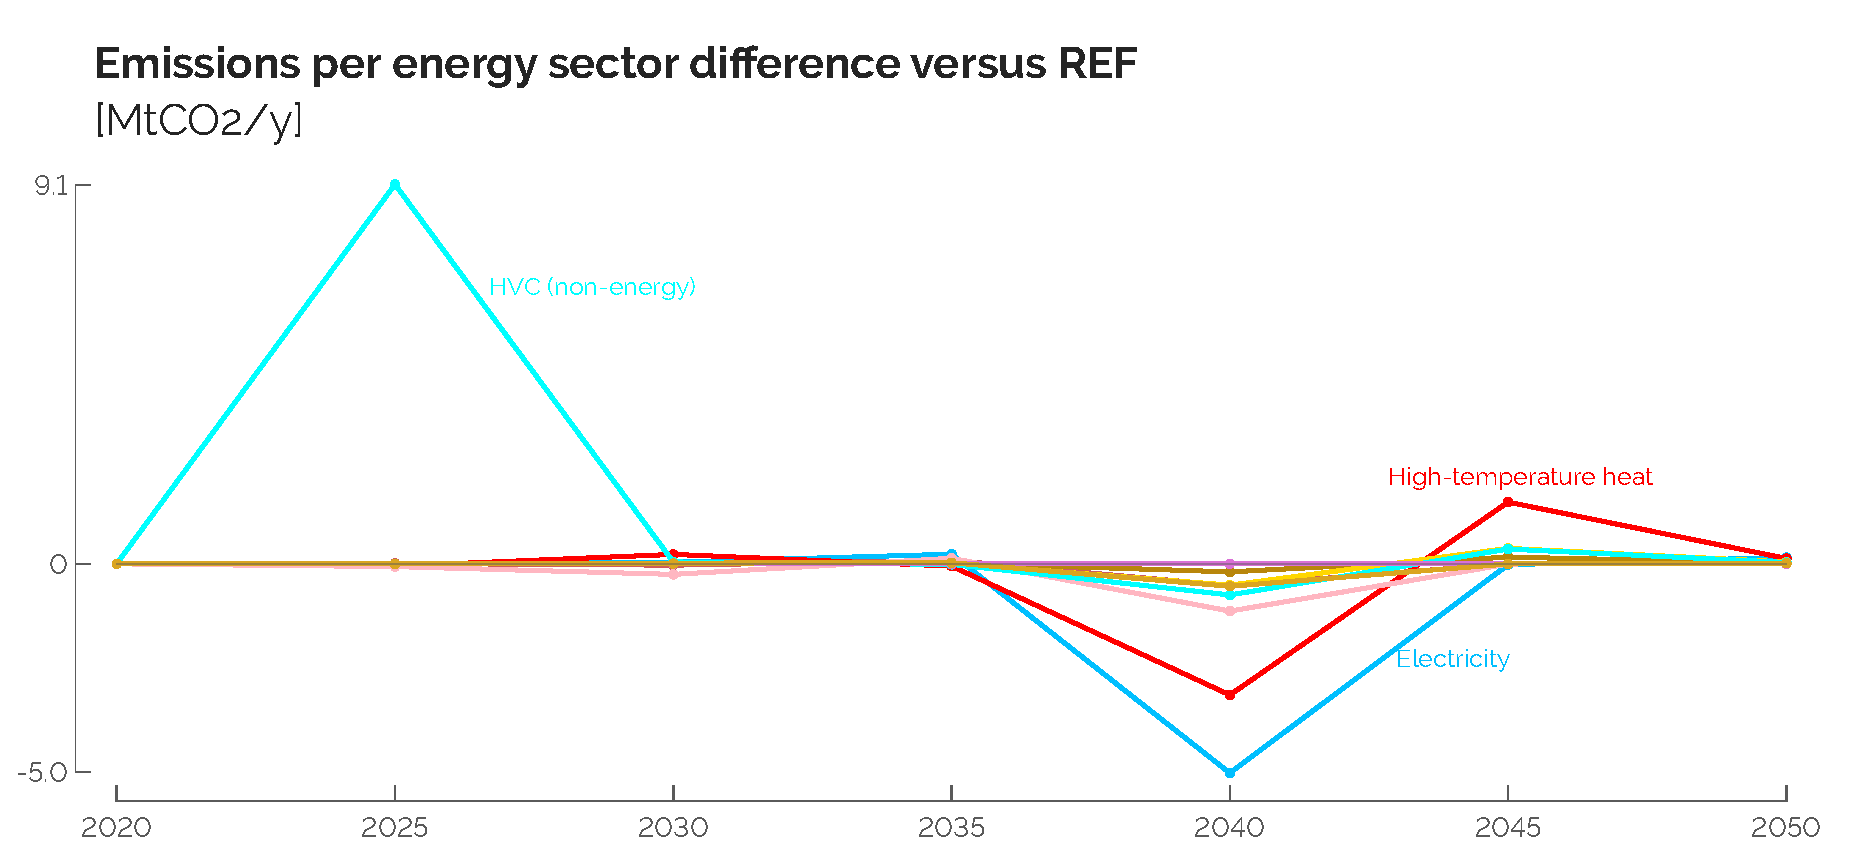
\includegraphics[width=0.8\textwidth]{GWP_per_sector_diff.pdf}
\caption{Emissions per energy sector differerence between the SMR and the REF cases. The deployment of \gls{SMR} from 2040 onward allows maintaining longer the use of \acrfull{LFO} for the production of \acrfull{HVC}.}
\label{fig:GWP_per_sector_diff}
\end{figure}

Then, considering the primary energy mix shown in \Cref{fig:results_deter_energy_mix}, three phases in the transition can be identified. Before 2040, thanks to the perfect foresight approach, the model finds it more economical in 2025 to keep on using 33.2\,TWh of \gls{LFO} to produce \gls{HVC} through naphtha/LPG-cracking. In 2040, uranium-driven \gls{SMR} substitutes the electricity originally produced from industrial \gls{CHP} and \gls{CCGT} running respectively on fossil gas and renewable ammonia. Finally, from 2045 onward, the significant drop in the consumption of electrofuels comes from the same industrial \gls{CHP}. This is the illustration of the atom-molecules dilemma where the consumption of local renewables is, on its side, not much affected. In other words, \gls{SMR} competes with importing electrofuels while both support the integration of local solar and wind energies. Then, like the power sector, the SMR case ends up in a less efficient whole-energy system by 2050 at it consumes 47\,TWh (+12.7\%) primary energy more to supply an unchanged \gls{EUD}. Interestingly, in both cases, given the assumptions made on the \gls{GWP} of the resources (\ie $\mathit{gwp}_{\mathrm{op,electrofuels}}=0$\,kt$_{\ce{CO2},\text{eq}}$/GWh and $\mathit{gwp}_{\mathrm{op,uranium}}=0.004$\,kt$_{\ce{CO2},\text{eq}}$/GWh), the constraint on the \ce{CO2}-budget leads to ``carbon-neutrality'' by 2050\footnote{The model being constrained to keep on using all the waste that would keep on being locally produced, the system in 2050 reaches a $\sim 3.5\,Mt_{\ce{CO2},\text{eq}}$/year.}.

\begin{figure}[htbp!]
\centering
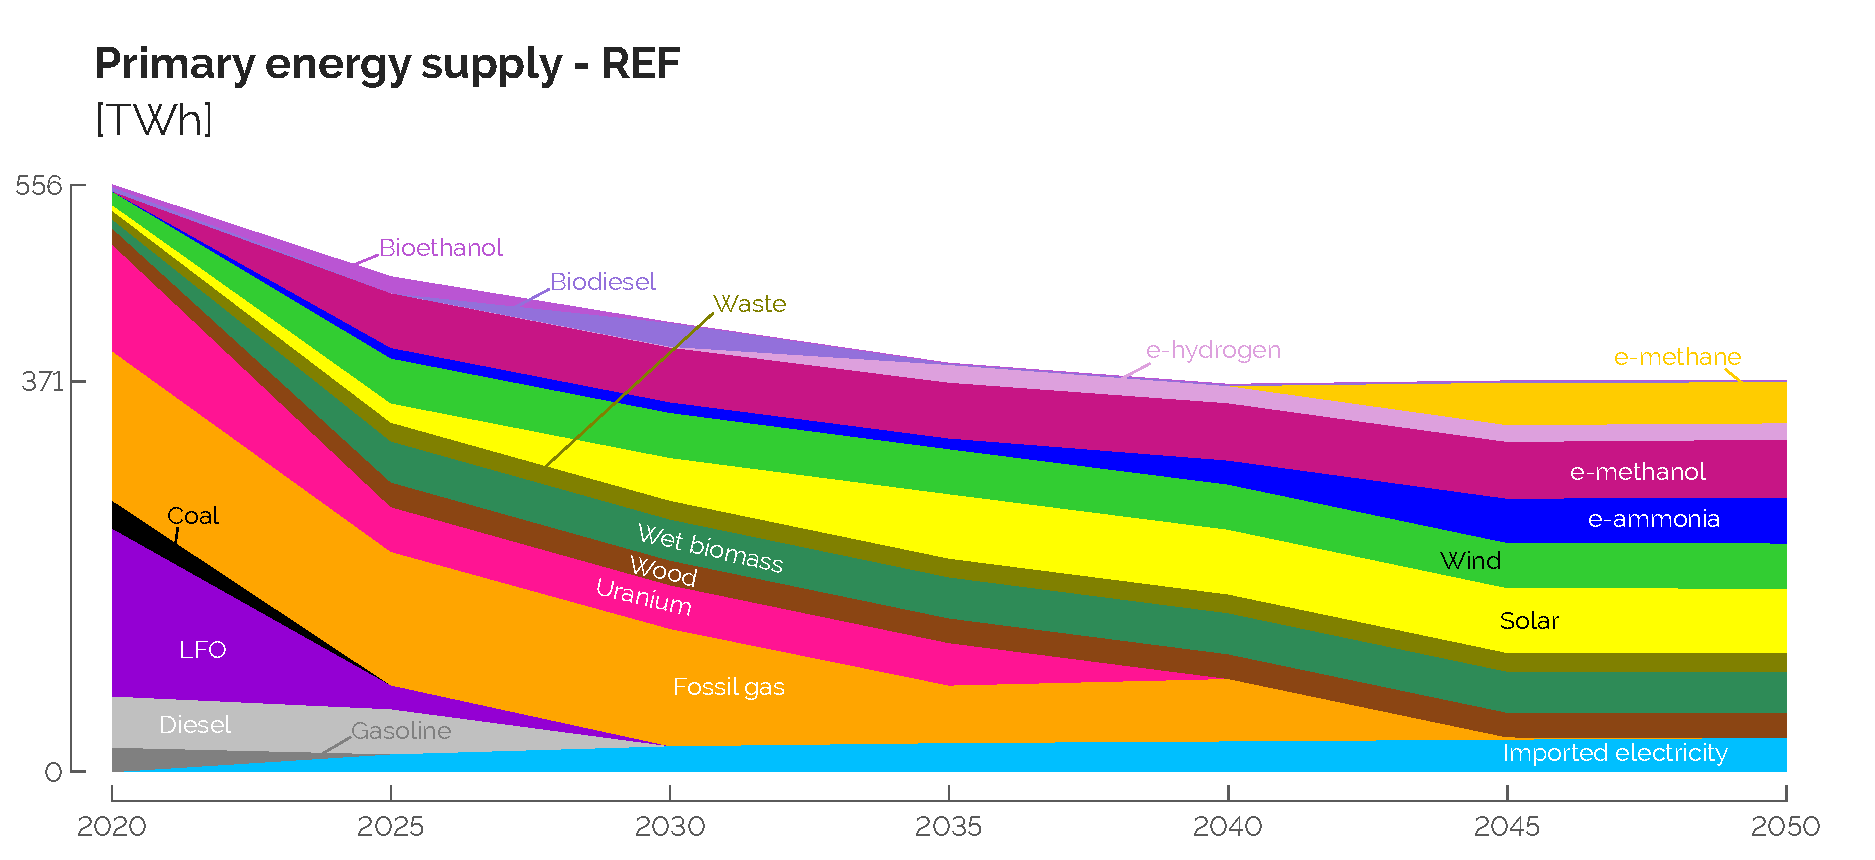
\includegraphics[width=0.8\textwidth]{Primary_mix_REF.pdf}
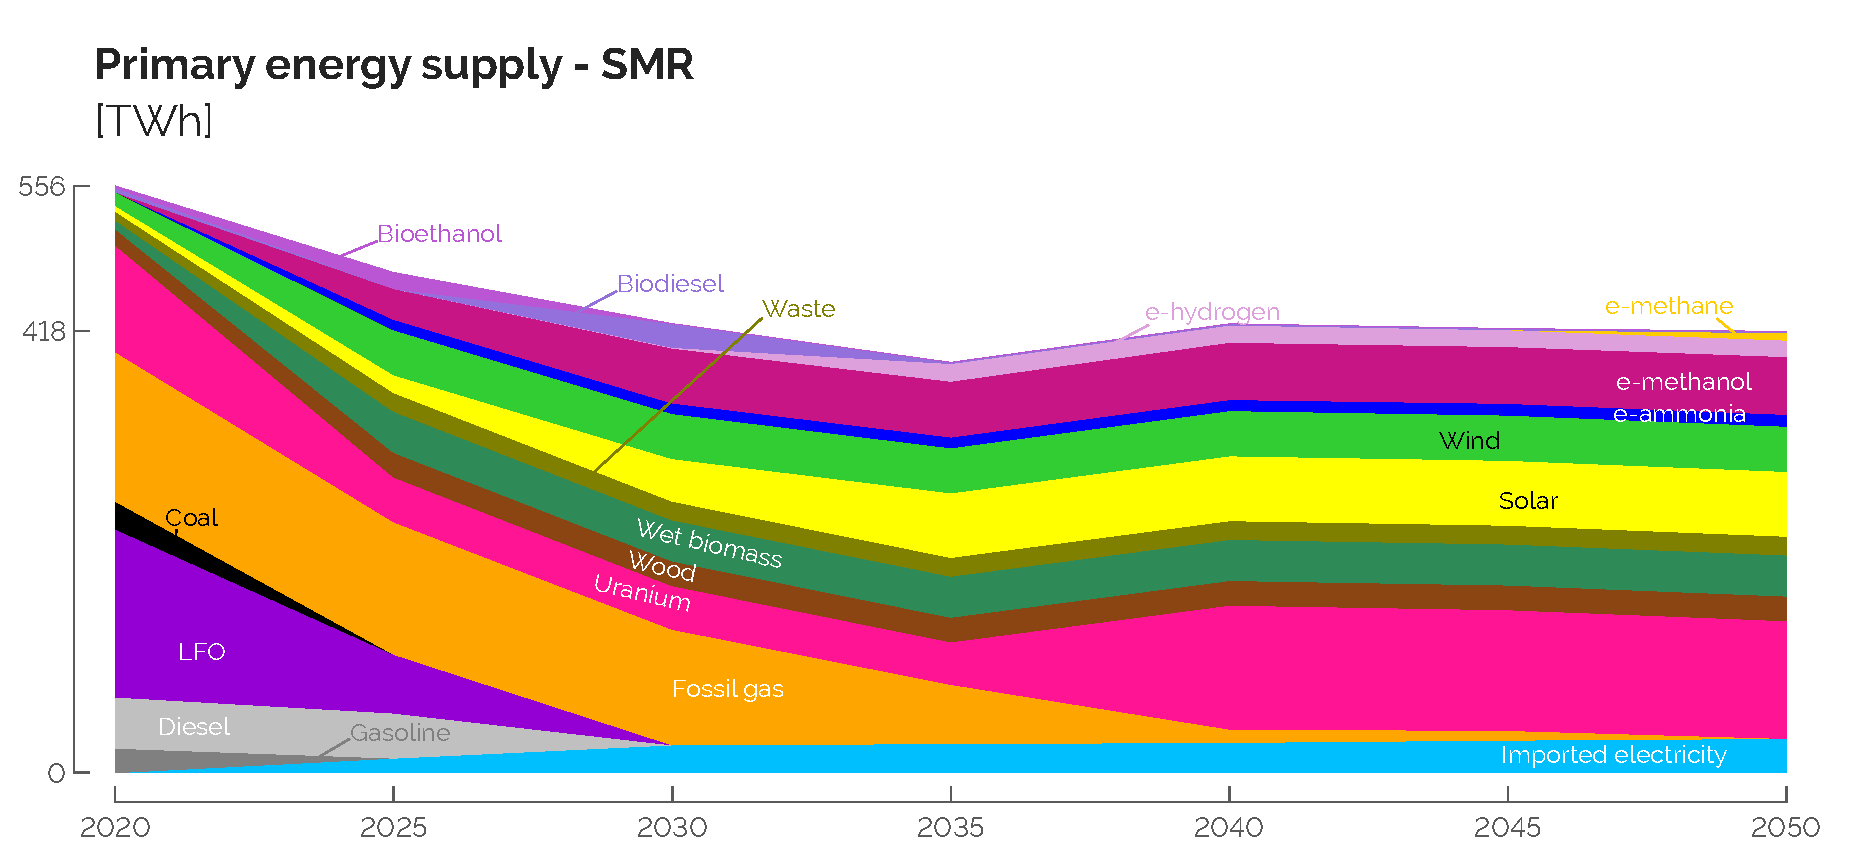
\includegraphics[width=0.8\textwidth]{Primary_mix_SMR.pdf}
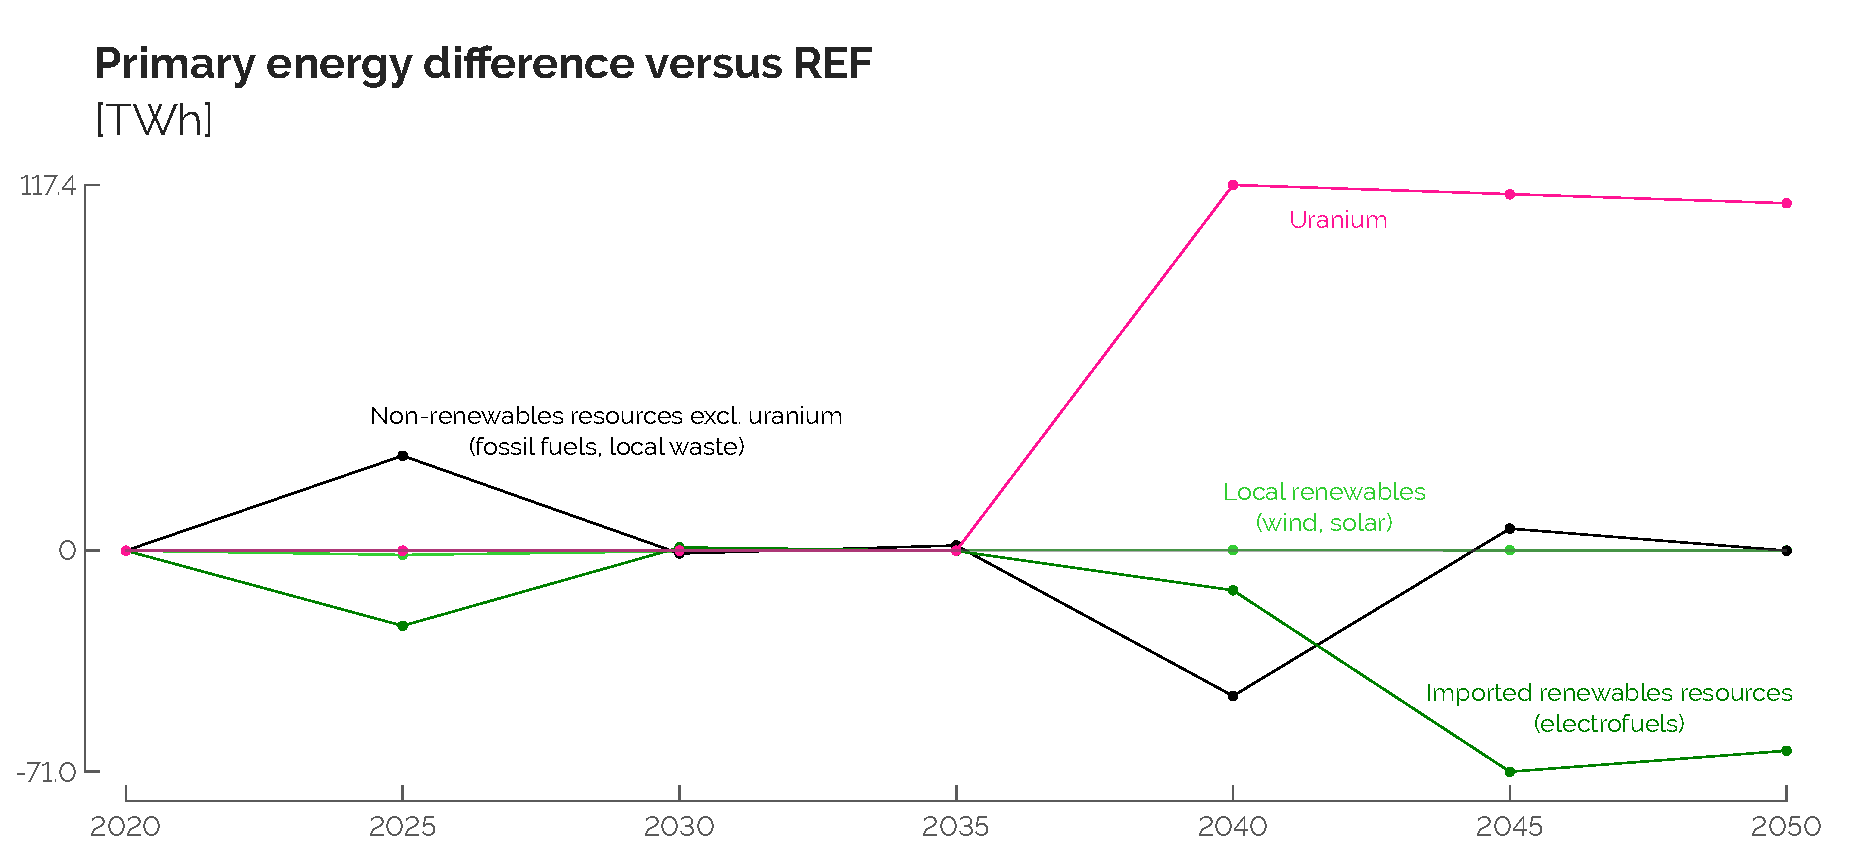
\includegraphics[width=0.8\textwidth]{Primary_mix_diff_uranium.pdf}
\caption{(Top) Primary energy mix over the transition for the REF and SMR cases. (Down) Difference of the mix between the two cases after aggregation per category. In line with \citet{rixhon2021terminology},uranium is considered as a non-renewable resource. It is nevertheless dissociated from other non-renewable resources for the sake of clarity. The imported electricity is split between imported non-renewable and renewable resources between the current share of renewables, \ie 37.41\% \cite{eurostat_share_re_elec}, and an assumed 100\%-renewable European electricity mix by 2050.}
\label{fig:results_deter_energy_mix}
\end{figure}

\subsection{Non-power sectors}
\label{subsec:atom_mol:results_deter_others}

Beyond the direct impact that \gls{SMR} has on the power sector, it also affects the other sectors. This is due to the sector-coupling typical of a whole-energy system optimisation \cite{contino2020whole}.\\

\myparagraph{High-temperature heat}\\

The main impact of including \gls{SMR} from 2040 onward on the high-temperature heat sector is (i) its higher direct electrification and (ii) the reduction of more efficient heat-and-power co-generation in the benefit of single-output industrial boilers. In the REF case, industrial electric heaters are mainly used to absorb, instead of curtailing, the ``over-production" of the 59\,GW solar-PV when fully deployed, in the sunny days. With \gls{SMR}, by 2050, an additional 1.7\,GW (+13\%) of these heaters can rely on a more constant supply of defossilised electricity. This increases the load factor (31\%) and yearly production (48\%) of these industrial electric heaters. Then, given the 44.6\,TWh of electricity produced by \gls{SMR}, cogeneration units are less relevant and, by 2050, 2.6\,GW industrial gas boilers completely substitute \gls{CHP} to produce 16.6\,TWh (\ie 23\%) of the total production of high-temperature heat.\\

\myparagraph{Low-temperature heat}\\

This sector is marginally impacted. In both cases, the major shift of supply from decentralised to centralised productions operates early in the transition, to hit the constraint that \gls{DHN} cannot supply more than 37\% of the \gls{LT}-heat production. Then, from a mix between oil (53\%), gas (43\%) and wood (4\%) boilers for the decentralised production of \gls{LT}-heat in 2020, the system shifts towards electric \gls{HP} only by 2035. Similarly for the centralised production of \gls{LT}-heat, electric \gls{HP} remains the most efficient and economic option.\\

\myparagraph{Mobility}\\

The passenger mobility is not affected either as the electrification of the system is preferentially done in this sector with \gls{BEV} substituting \gls{ICE} cars for the private sector by 2030. About the public mobility, trains and tramways supply their \textit{a priori} set maximum share, respectively, 50\% and 30\% complemented by \gls{CNG} buses substituting diesel-driven buses. Similarly, considering the freight transport, technology shifts (\ie from diesel to \gls{FC} trucks) or modal shares (\ie 53\%-47\% split between \gls{NG} and (bio)-diesel boats) are identical between the two cases.\\

\myparagraph{Non-energy demand}\\

The supply of ammonia (\ie from Haber-Bosch to direct import of renewable ammonia) and methanol (\ie import of renewable methanol) are unchanged between the two cases. However, as introduced previously, to produce \gls{HVC}, the full substitution of naphtha/LPG-cracking by \gls{MTO} is delayed as the emissions of the former are compensated by the later integration of \gls{SMR}.

\section{Uncertainty quantification on the cost, the atom and the molecules}
\label{sec:atom_mol:results_uq}
Besides the detailed understanding of the deterministic results, it is important to challenge these conclusions accounting for the uncertainty of the parameters \cite{guevara2020machine}. After briefly assessing the \acrfull{GSA} on the total transition cost (Section \ref{subsec:atom_mol:results_uq_cost}), this section investigates more deeply the atom-molecules dilemma (Section \ref{subsec:atom_mol:results_atom_mol}). The Sobol' indices are computed for import of renewable molecules and installed capacities of \gls{SMR}.

\subsection{Total transition cost}
\label{subsec:atom_mol:results_uq_cost}
Exhaustively listed in Appendix \ref{app:UQ_transition_cost}, \Cref{tab:UQ_short} gathers the most impacting parameters on the total transition cost. Per \citet{Turati2017}, parameters are considered as ``impacting'' if their Sobol' index is above the threshold $=1/d$, $d$ being the total number of uncertain parameters after the pre-selection phase. In this case, $d=34$, and, consequently, the threshold is equal to 2.9\%. \Cref{tab:UQ_short} shows that the cost of purchasing electrofuels is the most impacting parameter. On the contrary, the potentiality to install \gls{SMR} and its CAPEX have much lower influence on the variation of the total transition cost. Given the uncertainty characterisation presented in Section \ref{sec:cs:uncertainty}, there are 60\% chance that no \gls{SMR} could be installed. In other words, the variation of the parameter $f_{\mathrm{max,SMR}}$ has zero impact on the variation of the total transition cost in 60\% of the samples. Then, in perspective with the scenario analysis of Section \ref{sec:atom_mol:results_deter}, the 3.3\% reduction has been observed when \gls{SMR} is installed from 2040 onward. This represents only 10\% of the samples. Moreover, when it is possible, \gls{SMR} is always installed thanks to its characteristics: cheap and low-emitting fuel, the long lifetime leading to lower annualised CAPEX and higher salvage value. However, given its limited deployment, up to 6\,GW, \gls{SMR}-related parameters have a lower impact on the variation of the total transition cost. On the contrary, more expensive renewable electrofuels are always imported, to a smaller or larger extent depending on the sample. For instance, in the REF case (Section \ref{subsec:atom_mol:results_deter_overall}), the imported electrofuels represent, by 2050, 152.9\,TWh (\ie 41\% of the primary energy mix) with an average 93€/MWh cost of purchasing and, over the entire transition, a 273\,b€ cumulative OPEX (\ie 25\% of the total transition cost).

Given the relatively wide uncertainty range (\ie up to [-30.8\%; +24.0\%] by 2050) and, above all, the major share among the total demand, between 53\% and 60\%, the industrial \gls{EUD} is the second most impacting parameter. 

Then, as the driving factor for the annualisation and the salvage value of the assets, the interest rate has a 12\% Sobol' index. The model considers an overall interest rate for the entire system (\ie 1.5\% as a nominal value). In practice, the interest rate would vary depending on the technology investment risk. This variation would have, for instance, a major impact on the \gls{LCOE} of technologies like nuclear power plants \cite{world_nuclear_asso}, given the important capital needs and long time horizons \cite{IEA_Nuclear_2022}.

Finally, the cost of purchasing fossil fuels is also a key parameter in terms of variation of the total transition cost. However, due to the ambitious \ce{CO2}-budget, phasing out of fossil fuels is urgent and makes their impact smaller than their renewable alternatives.

\begin{table}[htbp!]
\caption{Total Sobol' indices of the uncertain parameters over the total transition cost. Where the cost of purchasing electrofuels is the top-1 parameter, \gls{SMR}-related parameters have a negligigble impact on this cost.}
\label{tab:UQ_short}
\centering
\begin{tabular}{l c c}
\toprule
\textbf{Parameter}  & \textbf{Ranking} & \textbf{Sobol' index} \\	
\midrule
\textbf{Purchase electrofuels} & 1 & 46.8\% \\
Industry EUD & 2 & 23.2\% \\
Interest rate & 3 & 12.0\% \\
Purchase fossil fuels  & 4 & 5.7\% \\
$\vdots$ & $\vdots$ & $\vdots$\\
\textbf{Potential capacity \gls{SMR}} & 11 & 0.9\% \\
$\vdots$ & $\vdots$ & $\vdots$\\
\textbf{CAPEX \gls{SMR}} & 33 & $<$0.1\% \\
\bottomrule							

\end{tabular}
\end{table}

\Cref{fig:UQ_PDF_total_transition_cost} shows the \gls{PDF} of the total transition cost given the 1260 samples. Stretching between 660\,b€ and 2050\,b€, the mean, the median and the nominal value (\ie REF case) are close to each other, respectively 1180\,b€, 1160\,b€ and 1080\,b€. Similarly to the analysis carried out by \citet{coppitters2023optimizing}, one observes here that the distribution is right-skewed. It could then be qualified as ``fragile" as the top 50\% of the samples cover a bigger range (\ie between 1160 and 2050) than the bottom 50\% of the samples (\ie between 660 and 1160). In other words, the bad scenarios, resulting in a total transition cost higher than the median, have a bigger effect on this cost.

\begin{figure}[htbp!]
\centering
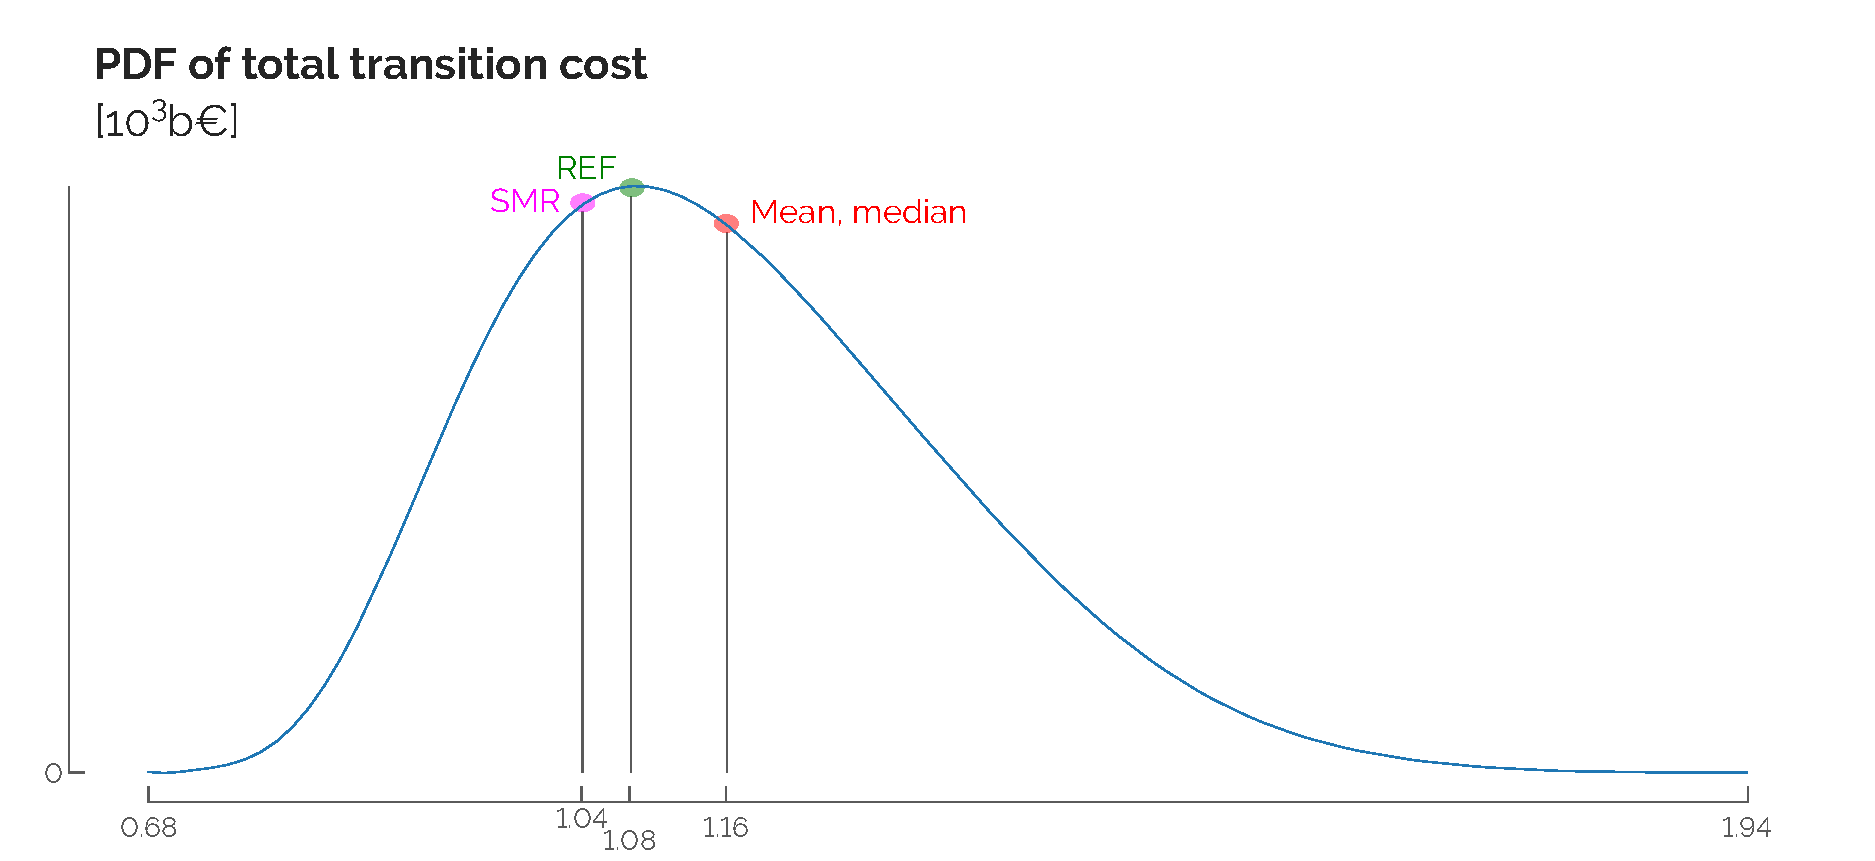
\includegraphics[width=0.8\textwidth]{UQ_PDF_total_transition_cost.pdf}
\caption{\acrfull{PDF} of the total transition cost. The mean, $\mu=1.18\cdot10^3$\,b€, is slightly higher than the median ($P_{50}=1.16\cdot10^3$\,b€) and the nominal cases cost, $1.08\cdot10^3$\,b€ and $1.04\cdot10^3$\,b€ respectively for the REF and SMR cases. Also, with a standard deviation, $\sigma=197$\,b€, a 95\%-confidence interval would be about [0.8; 1.6]$\cdot10^3$\,b€.}
\label{fig:UQ_PDF_total_transition_cost}
\end{figure}

\subsection{Atom and molecules}
\label{subsec:atom_mol:results_atom_mol}
The samples used to carry out the \gls{GSA} on the total transition cost, also provide the distribution of other outputs of the model like the import of renewable electrofuels over the transition. As the general trends are increasing, discrepancies exist between the different energy carriers (see \Cref{fig:results_uq_electrofuels}).
%
%\begin{figure}[htbp!]
%\centering
%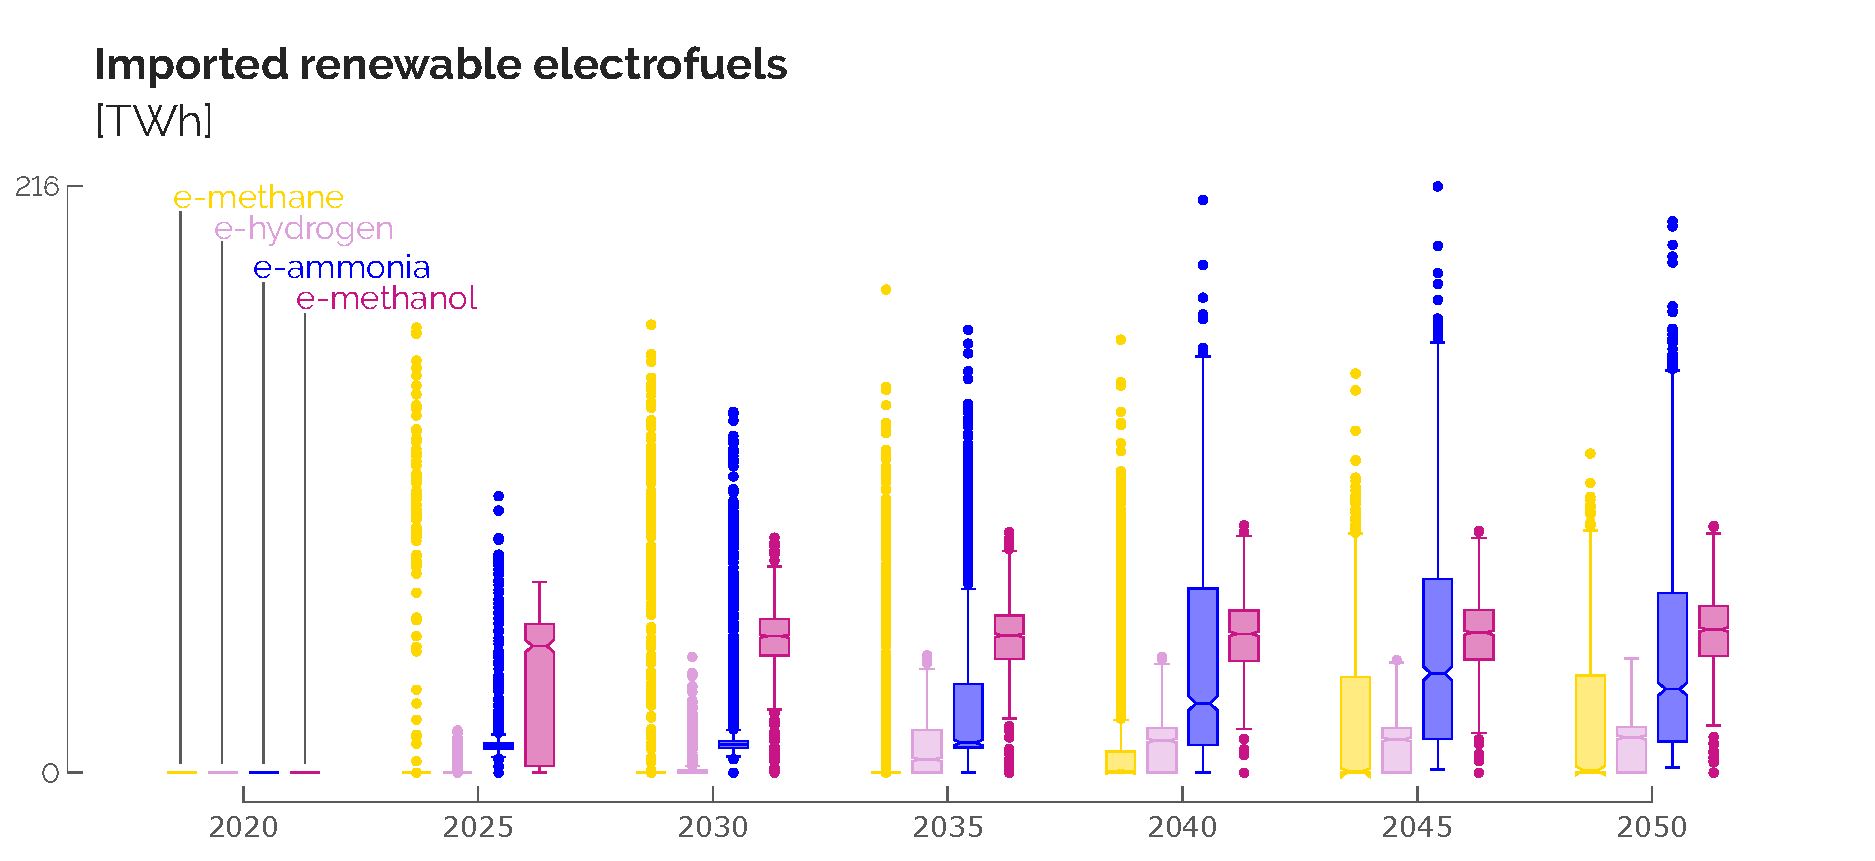
\includegraphics[width=0.7\textwidth]{UQ_Electrofuels.pdf}
%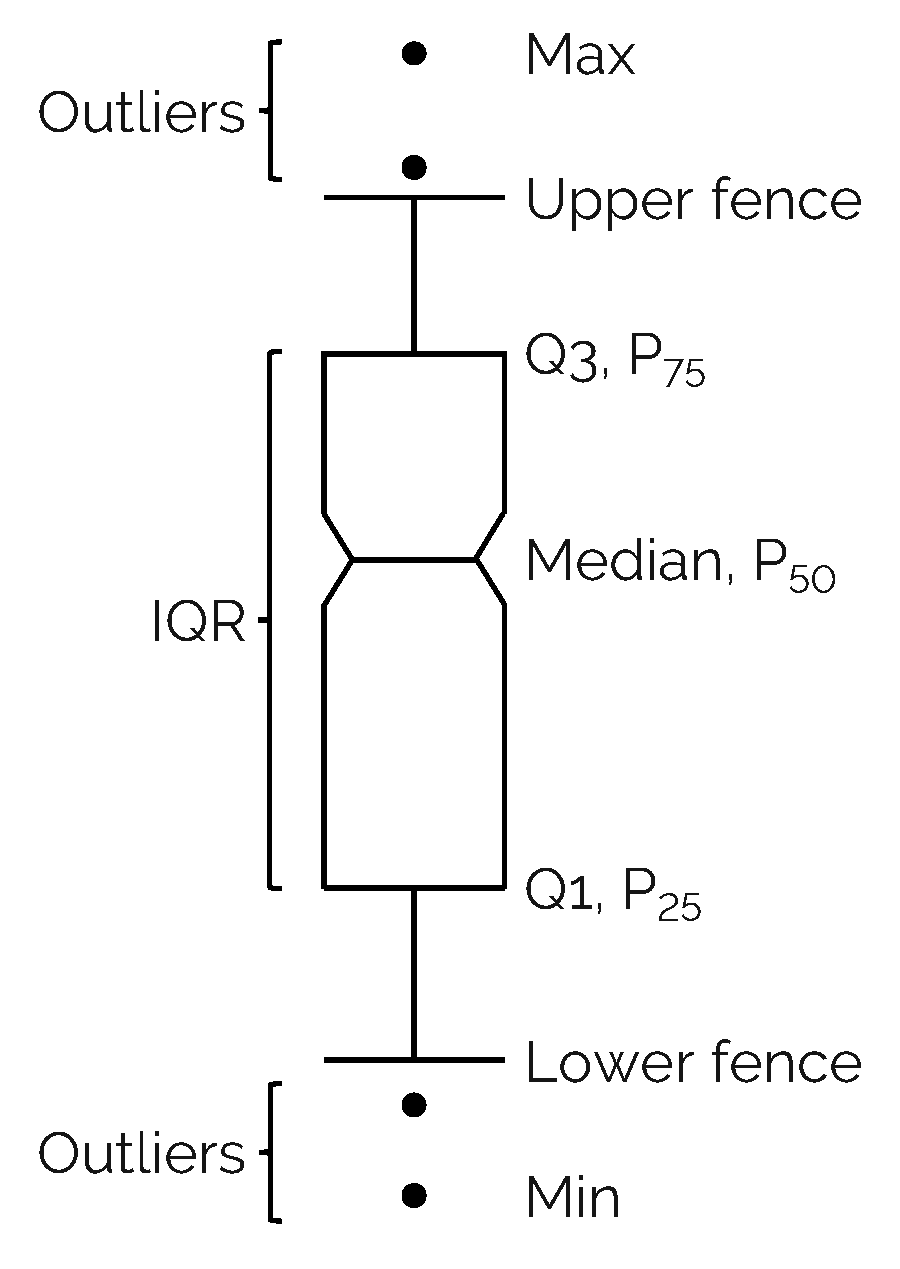
\includegraphics[height=4cm]{Schematic_boxplot.pdf}
%\caption{Distribution of the imported renewable electrofuels over the transition. Starting from no electrofuel in 2020, their respective import rises progressively along the transition (\ie increasing median) at different growth rates and with different ranges of values. Observations being either 1.5 times the interquartile range (IQR) less than the first quartile (Q1) or 1.5 times the interquartile range greater than the third quartile (Q3) are defined as outliers.}
%\label{fig:results_uq_electrofuels}
%\end{figure}

\begin{figure}[htbp!]
\centering
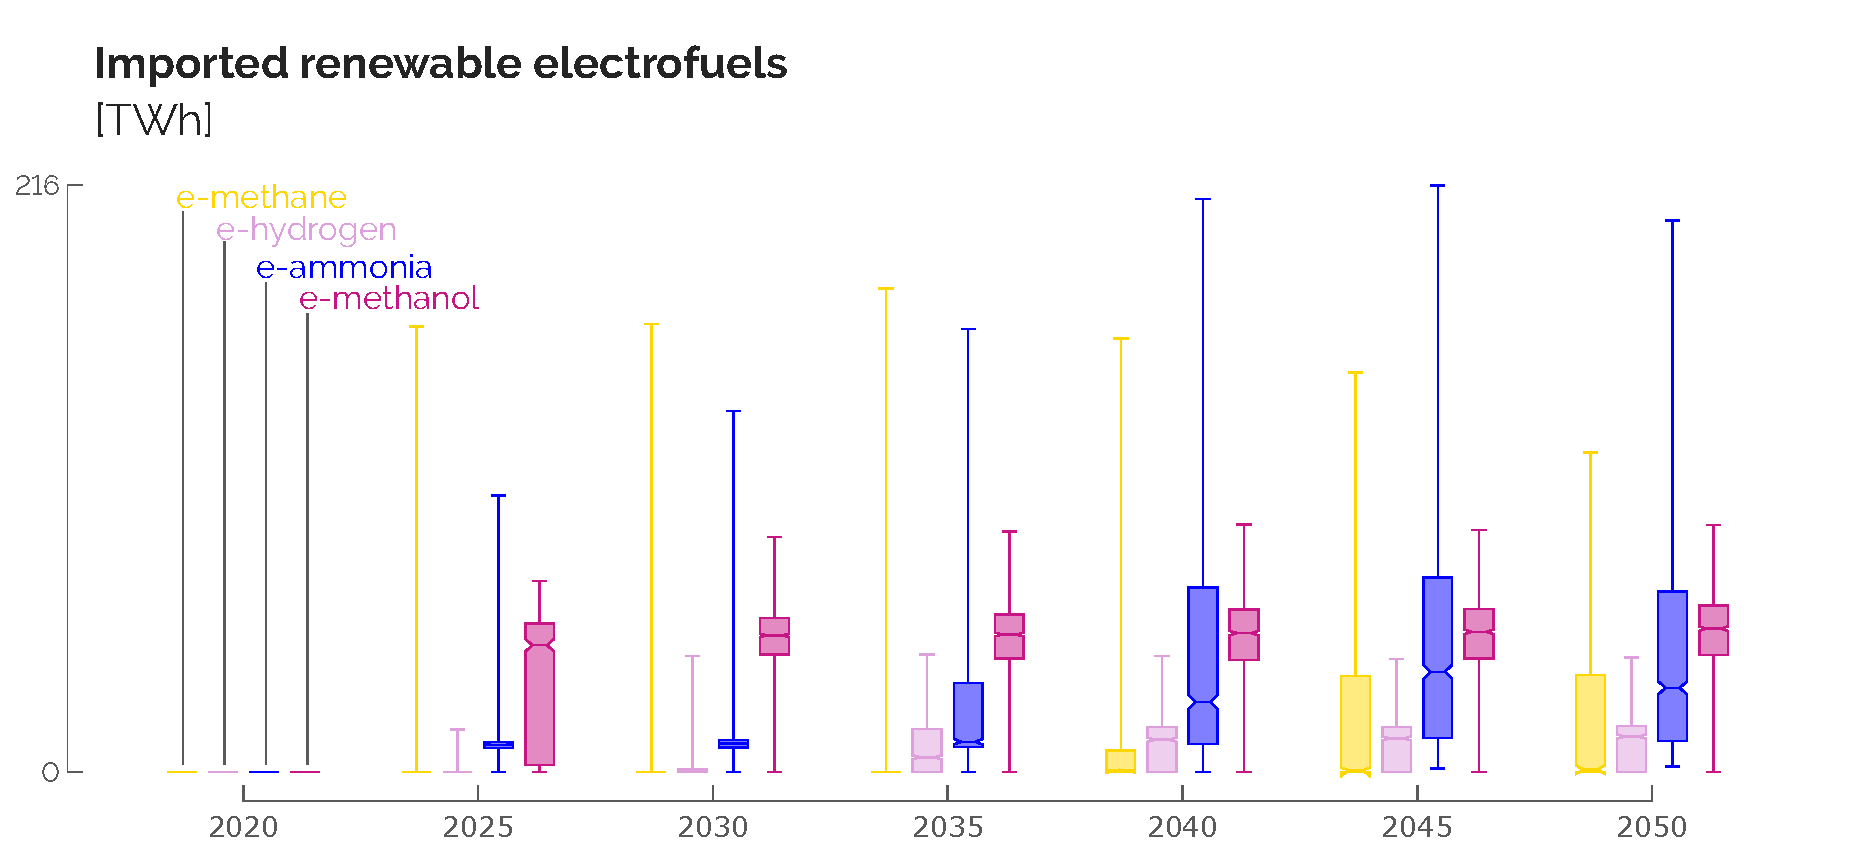
\includegraphics[width=0.7\textwidth]{UQ_Electrofuels_no_outlier.pdf}
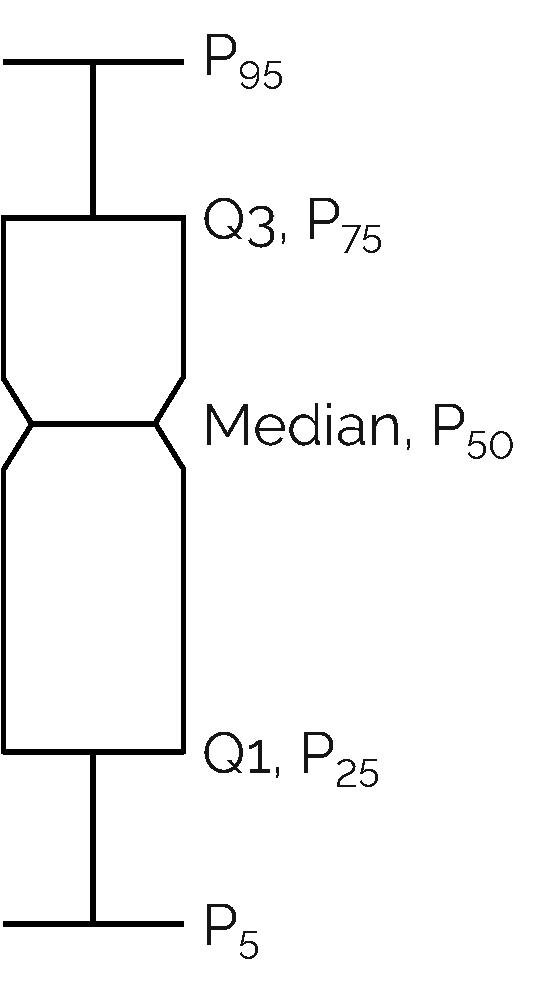
\includegraphics[height=3.8cm]{Schematic_boxplot_no_outlier.pdf}
\caption{Distribution of the imported renewable electrofuels over the transition. Starting from no electrofuel in 2020, their respective import rises progressively along the transition (\ie increasing median) at different growth rates and with different ranges of values. }
\label{fig:results_uq_electrofuels}
\end{figure}

E-methane, as the renewable alternative to fossil methane, substitutes it, sometimes at a very early stage of the transition, 2025, and large extent, 163\,TWh, which is more than 6\% more than the total import of electrofuels in the REF case. The necessity to import this molecule is progressive through the transition to supply mostly industrial \gls{CHP} and boilers. 

E-hydrogen becomes rapidly the main stream of hydrogen in the system, to reach a median and a maximum values of, respectively 13.0\,TWh and 42.1\,TWh in 2050. Hydrogen is more frequently used in the mobility sector. Like in the REF case, fuel cell trucks are often the first option but, in some outlying cases, fuel cell cars and buses appear to completely substitute respectively \gls{BEV} cars and \gls{CNG} buses by 2050. Moreover, some samples lead to local production of methanol via the methanolation process, to produce up to 17.8\,TWh of methanol (\ie 33\% of the total supply of methanol of the nominal REF and SMR cases). 

Then, the imported e-ammonia rapidly becomes cost-competitive against its fossil alternative (see Chapter \ref{chap:case_study}). At early stage of the transition, e-ammonia substitutes fossil ammonia and the Haber-Bosch process. Where the initial purpose of ammonia is to satisfy a relatively limited \acrfull{NED} (\ie 10 $\pm$ 3\,TWh by 2050), the variation of its import is mostly due to the higher or lower need for ammonia-\gls{CCGT} as a flexible option to produce electricity. From 2035, out of the four considered electrofuels, the imported e-ammonia is the one exhibiting the largest uncertainty with, for instance, an interquartile range (IQR)\footnote{The interquartile range is the difference between the third quartile ($Q3$ or $P_{75}$) and the first ($Q1$ or $P_{25}$). It is an indicator of statistical dispersion around the median, $Q2$ or $P_{50}$.} of about 50\,TWh. In some extreme cases, e-ammonia is the most imported molecules, \ie up to 216\,TWh or 58\% of the total primary mix. 

Likewise, e-methanol early becomes the selected option to supply methanol even though alternatives like biomass-to-methanol are selected to supply, on average, 5\% of the demand in methanol. Its \gls{NED} represents, on average, 3\% of the total consumption of methnaol. The variation of imported e-methanol is due to its role in the industrial production of \gls{HVC} through the \acrfull{MTO} process as it represents 95\% of the total consumption. For the remaining 2\%, methanol is also used to supply the freight transport sector via boats or trucks. More detailed statistics including the different sources of supply and consumption of gas, hydrogen, ammonia and methanol are provided in Appendix \ref{app:UQ_electrofuels}.\\

This part assesses the space of uncertainties, like \citet{pickering2022diversity} who investigated the space of feasibility to reach carbon neutrality in Europe. The trend lines of the key parameters can be drawn for these imports and the installed capacities of \gls{SMR} in 2050. We picked 2050 as it is the time of the transition where electrofuels, if imported, are imported in the largest amount compared to the other years of the transiton.Next to the name of a parameter, one can read its Sobol' index versus the output of interest. For these outputs of interest, different from the total transition cost, the \gls{LOO} error is around 20\%. Even though this is higher than the threshold of \SI{1}{\%}, the Sobol' indices allow ranking the most impacting parameters (see Section \ref{subsec:pce}). Box plots also point out the distribution of this output for the extreme low or high values of some parameters.

For the import of e-methanol, industrial \gls{EUD} is, by far (\ie $\sim$80\% Sobol' index), the key factor (Figure \ref{fig:results_uq_samples_methanol}). Due to its own \gls{NED} but, above all, since it is the low-emitting alternative picked by the model to supply the significant \gls{NED} of \gls{HVC}, the lower this demand, the lower the need to import e-methanol, and vice versa. 

\begin{figure}[htbp!]
\centering
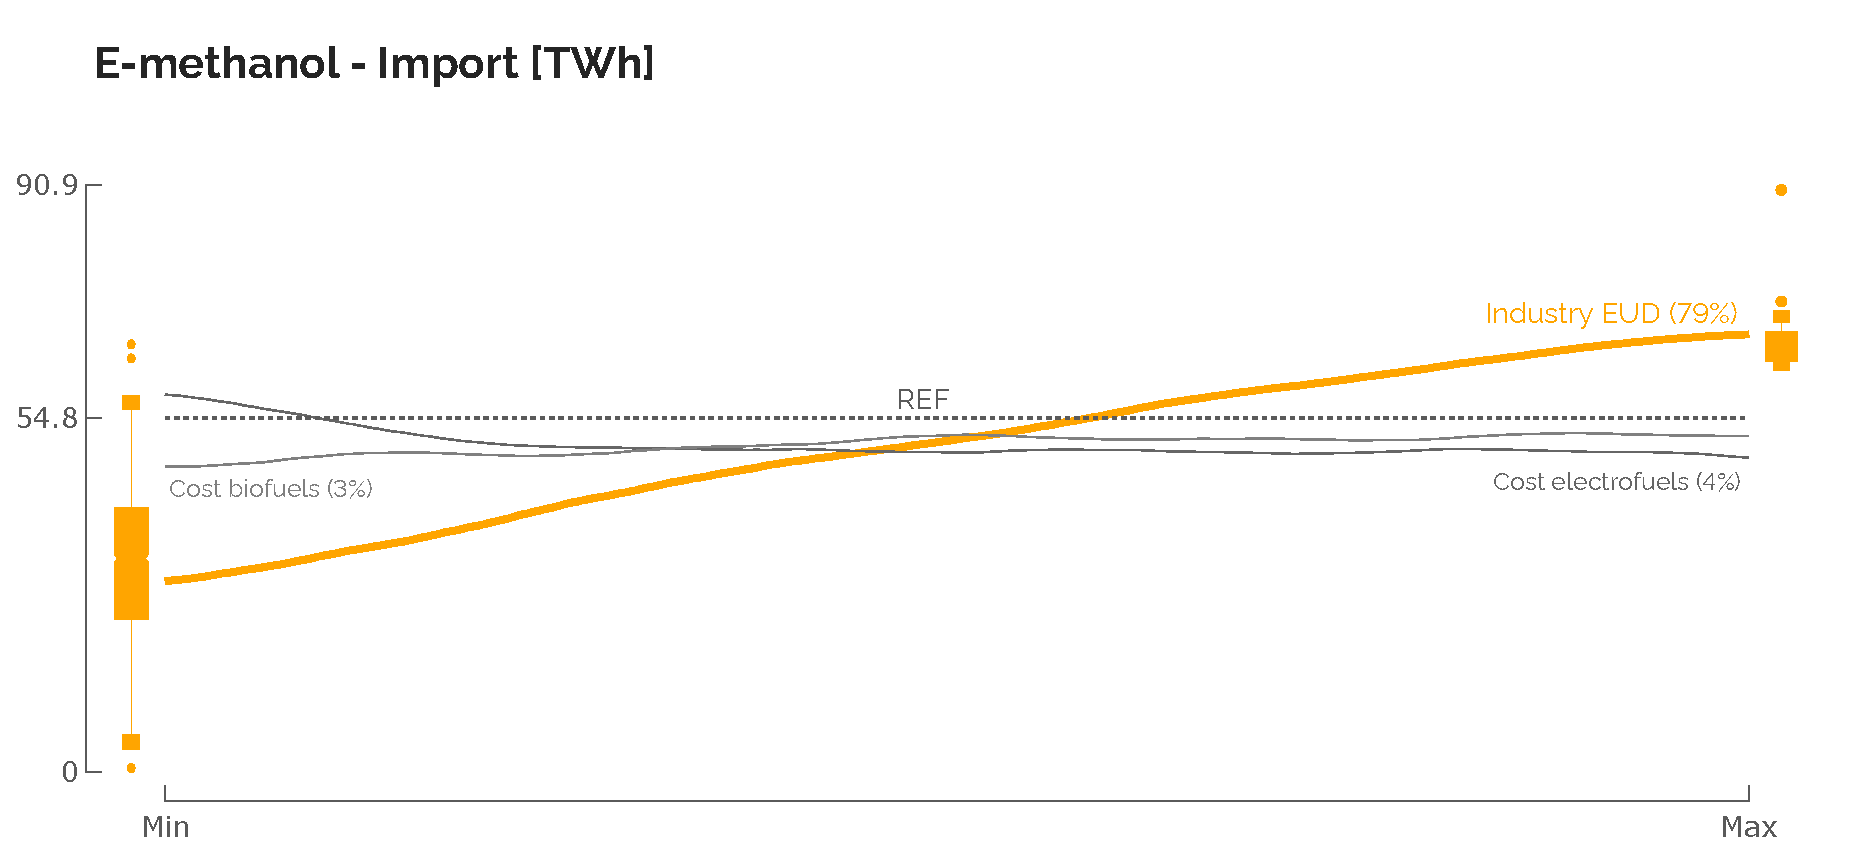
\includegraphics[width=0.8\textwidth]{UQ_Methanol_samples_2.pdf}
\caption{Trend lines of the key parameters on the import of e-methanol in 2050. Around these lines, box plots point out the distribution of the output of interest for the extreme values (either bottom-15\% or top-15\%) of some parameters. The grey dashed line gives the value of the output of interest in the REF case. }
\label{fig:results_uq_samples_methanol}
\end{figure}

As aforementioned, the industrial \gls{EUD} impacts the most the import of e-methane (Figure \ref{fig:results_uq_samples_gas}). This parameter directly dictates the demand of industrial high-temperature heat for which industrial gas \gls{CHP}, and industrial gas boilers to a lower extent, represent, on average over all the samples, respectively 25.6\% and 6.1\% of the total production. Then, considering the smaller-impact parameters, we notice that \gls{SMR} plays a non-negligible role. Indeed, if deployed, \gls{SMR} produces abundant low-emitting electricity for industrial electric heaters that substitute, even completely in some cases, gas alternatives. This confirms the observation made in Section \ref{subsec:atom_mol:results_deter_others}. Highly available local biomass also leads to smaller import of e-methane to supply bio-hydrolysis and produce methane-equivalent gas. Finally, and surprisingly, costs of purchasing electrofuels and fossil fuels have a positive and negative correlation with the amount of e-methane, respectively. In other words, by 2050, more expensive electrofuels result in more e-methane import. On the contrary, cheaper electrofuels result in higher import of fossil methane. Given the techno-economic optimum sought by EnergyScope, if electrofuels are more expensive, the system will, overall, import less of them, especially e-ammonia, mainly used by \gls{CCGT}. Subject to the \ce{CO2}-budget for the transition, the system goes towards more efficient technologies, like industrial methane-\gls{CHP} to substitute e-ammonia-\gls{CCGT} in the production of electricity. First running on fossil gas, these \gls{CHP} consume more e-methane by 2050. On the contrary, if electrofuels are cheaper, there is more import of them, and especially of e-ammonia. This leaves room for more emitting and cheaper resources to be used while respecting the \ce{CO2}-budget, \ie coal in industrial boilers that produce, in these cases, on average 24\% of the high-temperature (HT) heat in 2050. In these cases, the use of coal in 2050 highlights that, with a sharper decrease of the emissions at early stages in the transition, the model finds a solution including highly-emitting resources (\eg coal) while respecting the \ce{CO2}-budget. Consequently, there is smaller investment in methane \gls{CHP}, and consequently import of e-methane as more abundant renewable electricity is produced via e-ammonia-\gls{CCGT} and more HT-heat is supplied by industrial coal boilers. Even though we might expect that no more coal will be consumed in Belgium by 2050, the model still has the opportunity to use it if the \ce{CO2}-budget allows it. About the cost of purchasing fossil fuels, the parameter has mainly an impact on the import of fossil \gls{NG} as the most versatile energy carrier in the whole-energy system. If \gls{NG} is more expensive, the system will import less of it. Subsequently, the investments in methane-\gls{CHP} and boilers are more limited. This ends up in smaller need for e-methane by 2050.

\begin{figure}[htbp!]
\centering
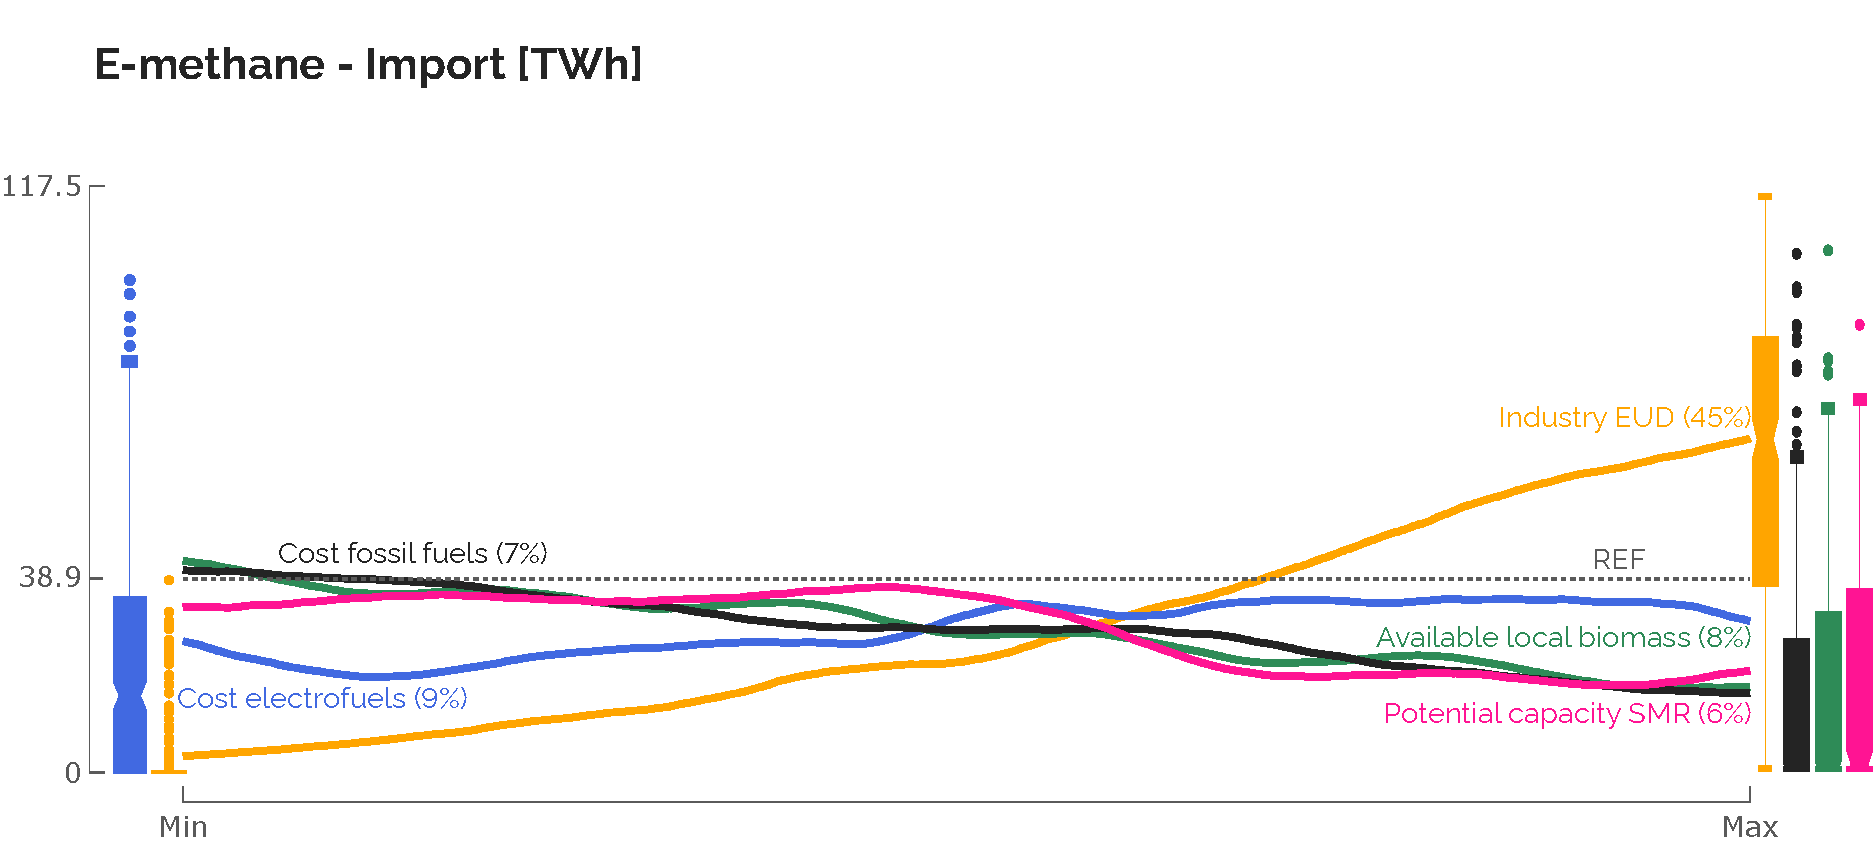
\includegraphics[width=0.8\textwidth]{UQ_Gas_samples_2.pdf}
\caption{Trend lines of the key parameters on the import of e-methane in 2050. Around these lines, box plots point out the distribution of the output of interest for the extreme values (either bottom-15\% or top-15\%) of some parameters. The grey dashed line gives the value of the output of interest in the REF case. }
\label{fig:results_uq_samples_gas}
\end{figure}

In relation to e-hydrogen, the sensitivity analysis highlights its dependence on various driving parameters, particularly those linked to the transport sector (Figure \ref{fig:results_uq_samples_H2}). The utilisation of e-hydrogen is most prevalent in \gls{FC} trucks, followed by \gls{FC} cars and buses to a lesser extent (Appendix \ref{app:UQ_electrofuels}). The adoption of fuel cell engines in trucks contributes, on average, to 63.5\% of the total road freight transport, thereby affecting the level of e-hydrogen imports. Consequently, the smaller is the CAPEX of fuel cell engines, the more the system imports e-hydrogen. Similarly, the cost of purchasing electrofuels influences e-hydrogen imports. Subsequently, the cost of purchasing biofuels emerges as the third most influential parameter. Indeed, biodiesel trucks are the mostly picked alternative to \gls{FC} trucks to provide, on average, 27.6\% of the total. Additionally, \gls{CNG} buses are preferred in public road transport (34.9\%), followed by \gls{FC} buses (11.2\%) competing with biodiesel and hybrid biodiesel buses, accounting for 27.8\% and 26.1\%, respectively. Finally, the last noticeable parameter at stake is the CAPEX of electric vehicles. In competition with \gls{BEV} that stand for 83.4\% on average of the private mobility sector, the cheaper these cars are, the more cost-competitive are these vehicles, and vice versa, versus \gls{FC} cars (\ie 13.7\% of the total passenger mobility, on average).

\begin{figure}[htbp!]
\centering
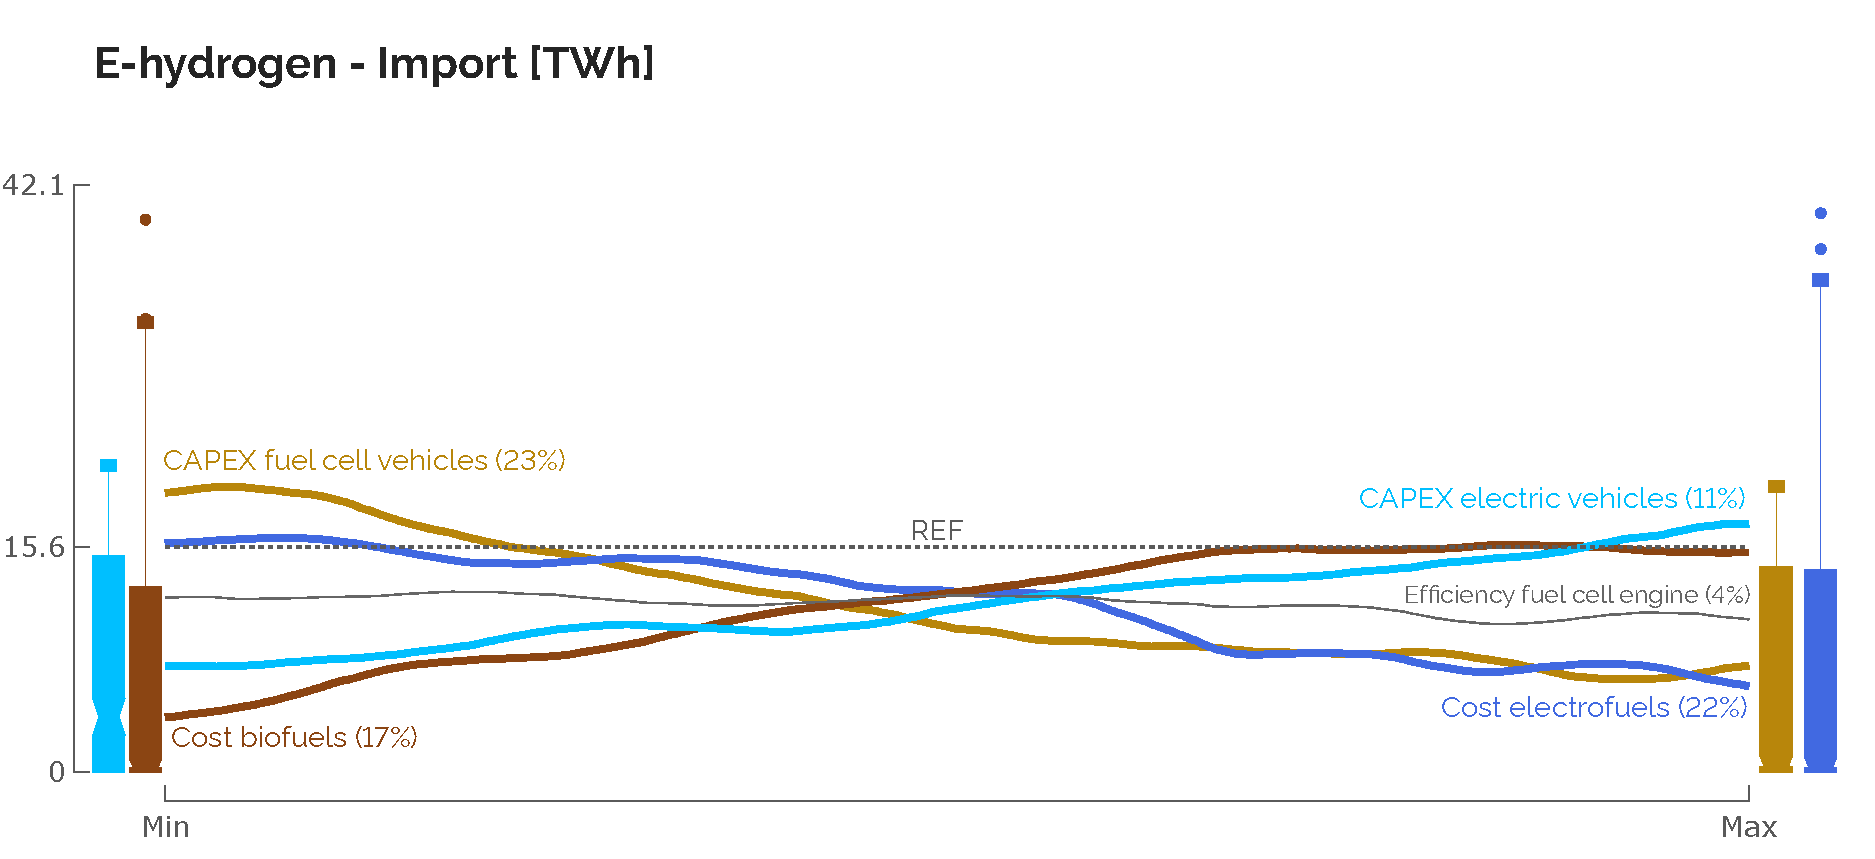
\includegraphics[width=0.8\textwidth]{UQ_H2_samples_2.pdf}
\caption{Trend lines of the key parameters on the import of e-hydrogen in 2050. Around these lines, box plots point out the distribution of the output of interest for the extreme values (either bottom-15\% or top-15\%) of some parameters. The grey dashed line gives the value of the output of interest in the REF case. }
\label{fig:results_uq_samples_H2}
\end{figure}

As already pointed out in Section \ref{subsec:atom_mol:results_deter_power_sector}, the installation of \gls{SMR} drastically reduces the import of e-ammonia (Figure \ref{fig:results_uq_samples_ammonia}). As ammonia \gls{CCGT} is the biggest consumer of ammonia by the end of the transition, low-emitting and cheaper electricity produced by \gls{SMR} (40 versus 151 €/MWh$_{\text{elec}}$) substitutes these \gls{CCGT}. With a higher cost of purchasing electrofuels, this import of e-ammonia drops down to 2.0\,TWh, 95.4\% less than in the REF case. Then, with a 12\%-Sobol' index, the cost of purchasing electricity from abroad, considered as renewable by 2050 and, therefore, a direct competitor to e-ammonia \gls{CCGT}, also affects the need of this molecule, especially when this cost is low.

\begin{figure}[htbp!]
\centering
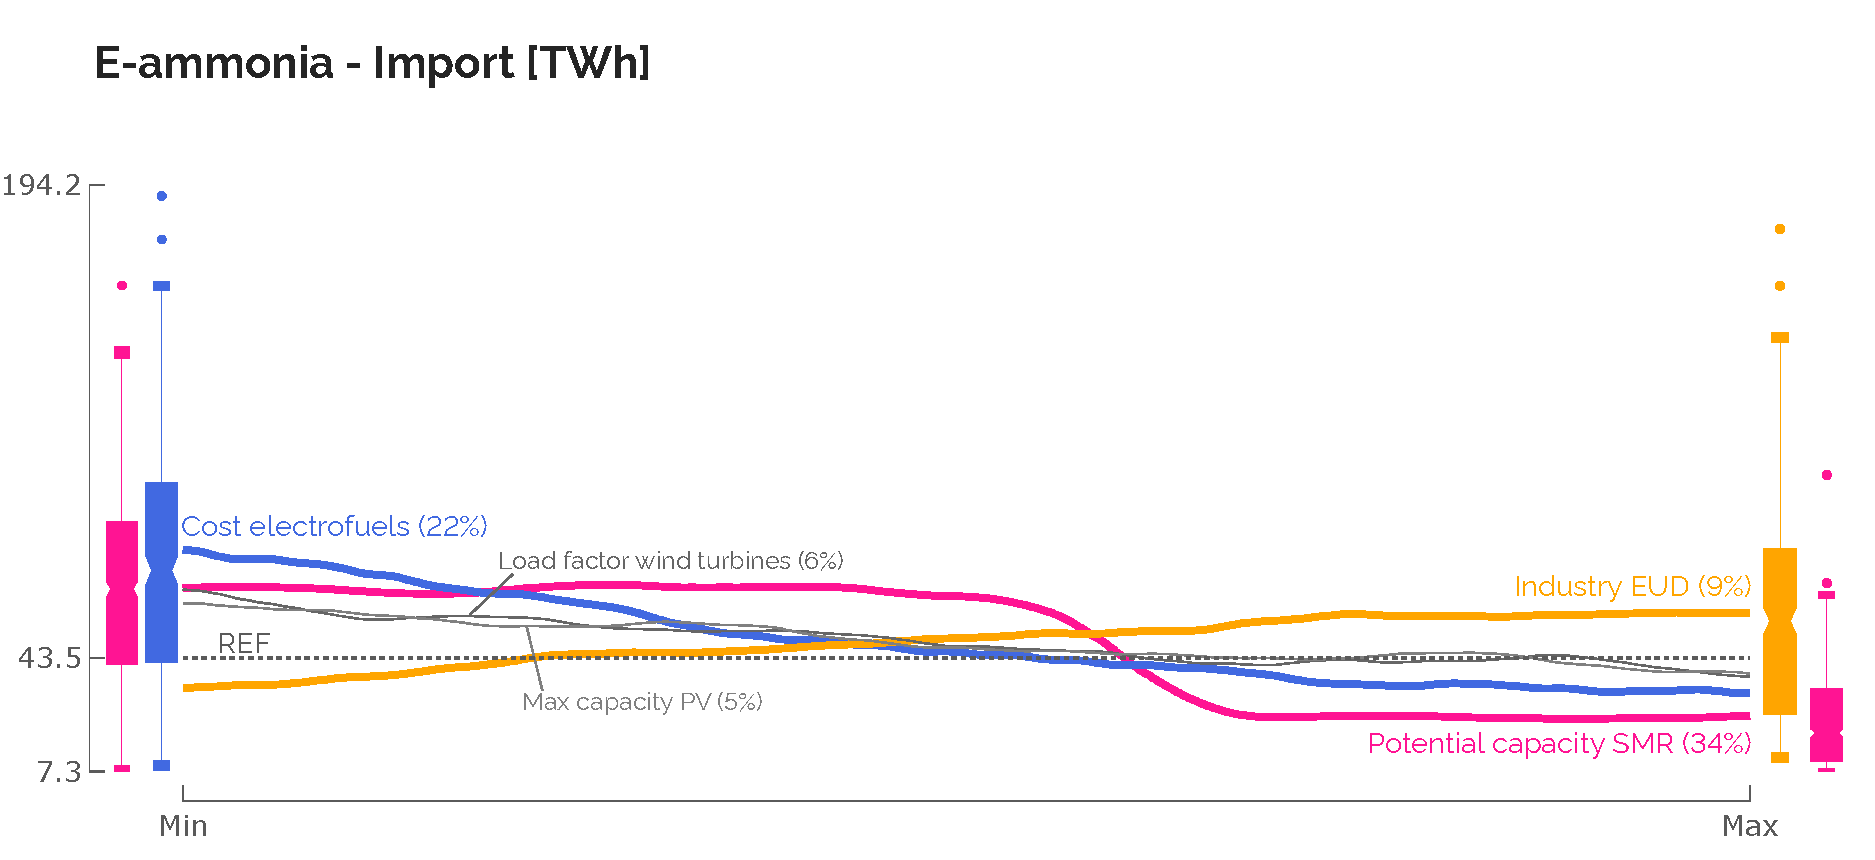
\includegraphics[width=0.8\textwidth]{UQ_Ammonia_samples_2.pdf}
\caption{Trend lines of the key parameters on the import of e-ammonia in 2050. Around these lines, box plots point out the distribution of the output of interest for the extreme values (either bottom-15\% or top-15\%) of some parameters. The grey dashed line gives the value of the output of interest in the REF case. }
\label{fig:results_uq_samples_ammonia}
\end{figure}

For the installed capacity of \gls{SMR}, it is the availability of the technology that drives its installation (Figure \ref{fig:results_uq_samples_SMR}). Not shown here but all the samples of the \gls{GSA} highlight that \gls{SMR} is installed to its maximum capacity, \ie 6\,GW, as soon as possible. In other words, the only parameter ``Potential capacity \gls{SMR}'' dictates the installation of this technology. In practice, we observe that as soon as this parameter is equal or higher than 0.9, 0.8 and 0.6, 6\,GW \gls{SMR} is installed from 2040, 2045 and 2050, respectively. Large range (-40\%; +44\%) of its CAPEX has a negligible impact on the installed capacity, with a Sobol' index of 0.9\%. This is explained by the long lifetime of the technology (60 years) and the salvage value recovered by 2050.

\begin{figure}[htbp!]
\centering
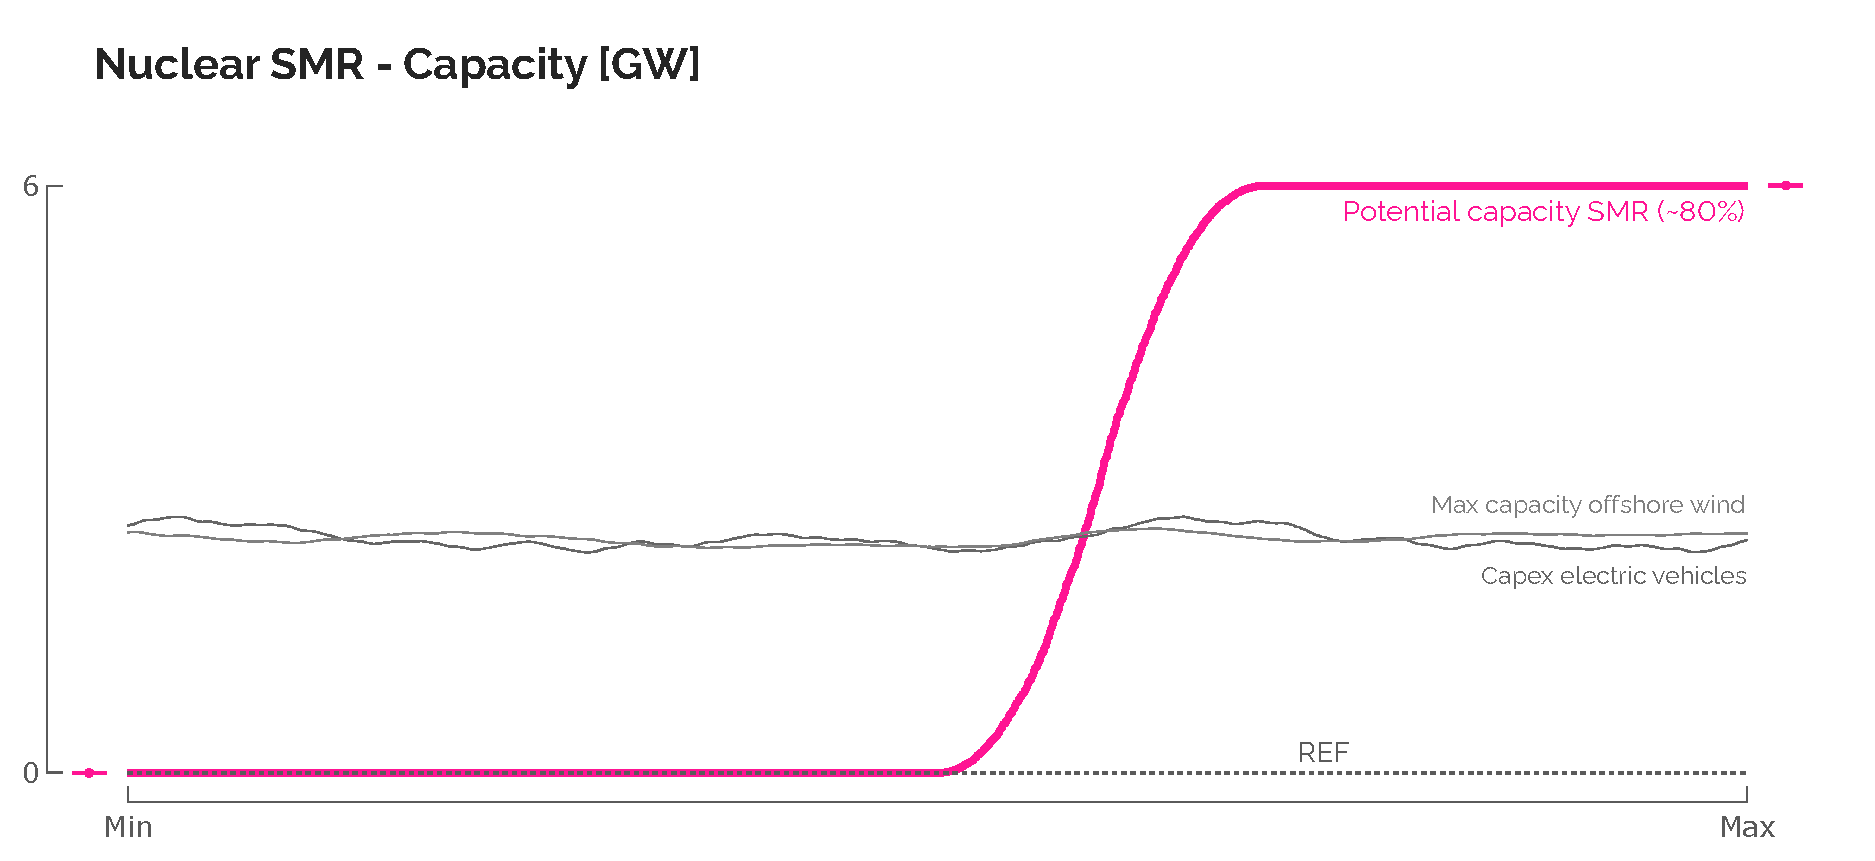
\includegraphics[width=0.8\textwidth]{UQ_SMR_samples_2.pdf}
\caption{Trend lines of the key parameters on the installed capacity of \gls{SMR} in 2050. Around these lines, box plots point out the distribution of the output of interest for the extreme values (either bottom-15\% or top-15\%) of some parameters. The grey dashed line gives the value of the output of interest in the REF case. }
\label{fig:results_uq_samples_SMR}
\end{figure}

\subsection{Local renewables}
\label{subsec:atom_mol:results_uq_VRES}
In line with results given in Section \ref{sec:atom_mol:results_deter}, the \gls{GSA} shows that \gls{SMR} has negligible impact on the deployment of local \gls{VRES} (\ie \gls{PV}, onshore and offshore wind turbines). Whereas the installed capacities of onshore wind is totally driven by the uncertainty on its maximum potential, Sobol' indices change for the most impacting parameters on the deployment of \gls{PV} and offshore wind (see Figure \ref{fig:results_uq_pdf_local_ren}). The key factor that drives the installed capacities of these two technologies is mostly their respective maximum potential, especially at the end of the transition, much more than their CAPEX. Given its higher \gls{LCOE} (\Cref{fig:LCOE}), \gls{PV} is more impacted in the short-term by the variation on the cost of purchasing electrofuels supplying e-methane (and e-ammonia to a lesser extent) \gls{CCGT}. However, this impact gets negligible by 2050.

\begin{figure}[htbp!]
\centering
\includegraphics[width=0.49\textwidth]{Sobol_PV.pdf}
\includegraphics[width=0.49\textwidth]{Sobol_WIND_OFFSHORE.pdf}
\caption{Impacting parameters on the deployment of \gls{PV} and offshore wind over the transition. Progressively, the impact of the uncertainty on the maximum potential increases, unlike the one on the cost of purchasing electrofuels.}
\label{fig:results_uq_pdf_local_ren}
\end{figure}


\section{Conclusions}
\label{sec:atom_mol:conclusions}
Given its lower \gls{LCOE} (40\,€/MWh$_{\text{elec}}$) and the important share of the investment recovered via its salvage value (between 79\% and 96\%), \gls{SMR} is installed as soon as available. It directly substitutes other flexible power generation units (\ie CCGT) and provides, by 2050, 44.6\,TWh, 25\% of the total electricity production. Consequently, this reduces the need to produce electricity via \gls{CHP} and allows increasing by 48\% the high-temperature heat produced by electric heaters. Besides these two sectors, the others (\ie low-temperature heat, mobility and non-energy demand) are marginally or not impacted by the integration of \gls{SMR}.

Given the ambitious \ce{CO2}-budget (\ie 30-year budget representing 10 years of the current emissions), the global sensitivity analysis highlights the biggest impact of the cost of purchasing electrofuels on the variation of the total transition cost, around 45\%. On the contrary, parameters directly related to \gls{SMR} (\ie its availability and its CAPEX) have limited impact, below 1\%. This \gls{GSA} also points out the key drivers for the import of renewable electrofuels and the installation of \gls{SMR} by 2050. Besides the cost of purchasing electrofuels (\ie the lower this cost, the bigger the imports), it shows that available \gls{SMR} would have mainly a direct impact on e-ammonia, by substituting the ammonia \gls{CCGT} that is the biggest consumer of this molecule. Indirectly, this parameter will also reduce the import of e-methane by reducing the need for gas \gls{CHP} and gas boilers. About e-hydrogen and e-methanol, their imports are impacted by the other technologies in competition in the transport sector and the industrial demand, respectively.

In conclusion, this work puts under the spotlight the ``competition'' between \gls{SMR} and imported electrofuels while both of them support the integration of local \gls{VRES}. Betting on \gls{SMR} means letting the emissions go up at early stages of the transition (\ie \gls{LFO} still used in 2025 to produce \gls{HVC}) to end up with an overall transition and a system by 2050 that are 3.3\% and 8.8\% cheaper than in the REF case, respectively. However, given the need to import molecules at earlier stages of the transition, with or without \gls{SMR}, it seems reasonable to keep on investing in the transport and the infrastructure to support these imports. This would allow covering ourselves against the risk of eventually not having \gls{SMR} available by the end of the first half of this century. The perfect foresight approach does not model this risk as the possibility to install or not \gls{SMR} is known in advance. In the EnergyScope Pathway model, assuming the same technology mix as in the SMR case up to 2040 but without installing \gls{SMR} for the rest of the transition, \ie between 2040 and 2050, would require drastic (and quick) changes to still meet the \ce{CO2}-budget: around 44\,b€ of additional cumulative OPEX in purchasing electrofuels, mostly e-ammonia (+32\,TWh by 2050) and e-methane (+31\,TWh) to supply \gls{CCGT} and industrial \gls{CHP}. As a more concrete example, Fluxys, the manager of the gas network in Belgium, already presents significant investments by 2032 (\ie 1.3\,b€) to support this transition in the near future \cite{Fluxys_2023}. 

Chapters \ref{chap:chap_RL} and \ref{chap:chap_RobPol} put in practice the methodology detailed in Chapter \ref{chap:chap_methodo} to come up with a policy to get a system robust to this possibility of finally not having access to \gls{SMR}, as well as other uncertainties, especially when considering a myopic progression through the transition.
\clearpage

%%% -- Chapter 4 - UQ on pathway and focus - Atom versus molecules -----------------------------
%\clearemptydoublepage
%\chapter{From a perfect foresight to a myopic optimisation of the pathway} 
%\label{chap:chap_myopic}
%%!TEX root = ../thesis_main.tex
%!TEX encoding = UTF-8 Unicode
In this chapter, I highlight the advantages of the myopic pathway, the methodological adaptations needed to have a myopic optimisation from EnergyScope Pathway perfect foresight and detail the difference with the perfect foresight for the case study. 

\section{Why and how myopic}
\label{sec:chap3_why_how}
Besides the fact that it is a necessary framework for the application of RL,  explain here why it is interesting, as is, to consider myopic optimisation (time saving, more appropriate to mimic policymakers' shortsightedness, etc.)

Detail the little tweeks to go from a perfect foresight to a myopic optimisation, in terms of implementation.

\section{Case study and results: Belgian energy system under \ce{CO2} trajectory}
\label{sec:chap3_case_study_results}

\subsection{Case study}
{\color{red}Question to HJ and FC : J'hésite sur le cas de référence pour la comparaison en termes de trajectoire \ce{CO2}. Voici ce à quoi je pense:
\begin{enumerate}
\item Comme ce qu'on a présenté dans le papier Pathway, une décroissance linéaire entre les émissions de 2020 et la neutralité carbone en 2050
\item Sur base du budget \ce{CO2} identique à celui de la décroissance linéaire (~1.9Gt\ce{CO2}), imposer au myopique la trajectoire \ce{CO2} issue de l'optimisation perfect foresight. Dans cette option, il y a deux sous-choix:
\begin{itemize}
\item Imposer la neutralité carbone en 2050, comme dans le cas 1.
\item Ne pas imposer la neutralité carbone en 2050
\end{itemize}
\item Sur base du budget \ce{CO2} que je donne implicitement comme objectif à mon agent (~1.2Gt\ce{CO2}), imposer au myopique la trajectoire \ce{CO2} issue de l'optimisation perfect foresight. Dans cette option, il y a deux sous-choix:
\begin{itemize}
\item Imposer la neutralité carbone en 2050, comme dans le cas 1.
\item Ne pas imposer la neutralité carbone en 2050
\end{itemize}
\end{enumerate}
Perso, je choisirais de me rapprocher le plus possible de ce que je fais ensuite avec l'agent. Du coup, ce serait le cas 3  sans imposer la neutralité carbone 2050. Dans ce cas, pour l'avoir observé, le modèle n'atteint pas la neutralité carbone. 

Quel est votre avis sur la question?
}

Define the case study and the \ce{CO2} trajectory. 

\subsection{Results and comparison with Perfect foresight}

\subsection{Discussion and perspective with the literature} 
%\clearpage


% -- Chapter 4 - Reinforcement Learning -
\clearemptydoublepage
\chapter{Reinforcement Learning \ce{CO2}-policy robust optimisation}
\label{chap:chap_RL}
\vspace{-0.2cm}
\begin{flushright}
\emph{``For the things we have to learn before we can do them, we learn by doing them.''}\\
Aristotle, in \textit{The Nicomachean Ethics}, IV$^\text{th}$ century BC
\end{flushright}
\vspace{0.4cm}

Uncertainties about the future along with a large variety of \gls{IAMs} yield an even larger variety of \gls{GHG} emissions reduction pathways \cite{nicolas2021robust}. For instance, several studies \cite{IPCC_CO2_budget,steffen2018trajectories} advocate for actions to take in the near future, especially to keep on track within the 1.5°C (if not, 2°C) increase of global temperature above pre-industrial levels by the end of the century. On the contrary, using his top-down model DICE, \citet{nordhaus2014question} states that immediate and drastic actions are not compulsory to meet the ambition of climate change mitigation. 

To navigate through the myopic transitions not constrained by a prescribed \ce{CO2}-trajectory and investigate the efficiency of different policies, we apply the reinforcement learning approach detailed in Section \ref{sec:meth:RL} on the case study of Belgium. Besides the environment, \ie the myopic transition pathway of the whole-energy system via EnergyScope Pathway (see Chapter \ref{chap:chap_methodo}), the first part of this chapter presents the three key features of interaction between the agent, optimizing its policy, and the environment: actions, states and reward.  Then, the results of this policy optimisation point out strategies to follow, \ie \textit{sweet spots}, in the transitions under uncertainties as well as \textit{no-go zones} where the chances of succeeding the transition, \ie respecting the \ce{CO2}-budget, are very limited. Finally, these results are compared with references, \ie the perfect foresight and the myopic optimisation of the transition under the same uncertainties but without the trained \gls{RL}-agent that can support this transition thanks to its learned policy.

\section*{Contributions}
\label{sec:RL:contributions}
Applying the \gls{RL} approach to the optimization of the myopic transition pathway of a whole-energy system presents several novelties. First of all, as introduced in Section \ref{subsec:meth_RL_fundamentals}, when applied to energy systems, \gls{RL} is more dedicated either to smaller scale systems (\eg \gls{BEMS}, vehicles and energy devices) or to sector-specific, often the power sector, problems (\eg dispatch problems, energy markets and grid) \cite{perera2021applications}. In our case, the sector-coupling, the long-term goal at the end of a multiple-steps transition and the number of uncertain parameters make this application new for \gls{RL}.

Applying \gls{RL} to the optimisation environment of EnergyScope Pathway myopic,  rather than a simulation environment, allows building a hierarchical multi-objective optimisation framework: while the objective of the environment remains the minimisation of the total ``transition'' cost (on the concerned limited time window), the agent optimises its strategy to respect the \ce{CO2}-budget. 

Comparing the \gls{RL}-based results with more conventional approaches, \ie perfect foresight optimisation, highlights the added-value brought by this approach in the exploration of myopic transition pathways.

Usually, applications of \gls{RL} focus more on the result of the learning process, the optimised policy, for optimising the control of a system \cite{perera2021applications}. This thesis also investigates the learning episodes themselves to explore the field of possibilities to succeed the transition.


\section{Definition of the actions, reward and states}
\label{sec:RL:act_states_rew}
As already introduced in Section \ref{subsec:meth_RL_algo}, the environment with which the \gls{RL}-agent interacts is the optimisation of the transition pathway of a whole-energy system on a specific time window, \eg 2020-2030 then 2025-2035 and so on, until 2040-2050 (see Figure \ref{fig:Schematics_RL}). In a nutshell, starting from the initial state of the environment (\ie the whole-energy system in 2020), the agent takes a set of actions that influence the environment, \ie that affects parameters of the Linear Programming in EnergyScope Pathway. Then, the window 2020-2030 is optimised via EnergyScope. Some of the outputs of this optimisation feed the agent with either the new state of the system or the reward, \ie telling the agent how good the actions were at the state he took it. Based on the new state and the reward, the agent takes another set of actions and the window 2025-2035 is optimised. This goes on until 2050.

\subsection{Actions}
\label{subsec:RL:act_states_rew:act}

Defining the levers of action, the core of the policy, to support the transition of a country-size whole-energy system is challenging, especially when accounting for political and socio-technical aspects \cite{castrejon2020making}. In our work, focusing only on the techno-economic aspect, we assume that the actions taken by the agent are directly implemented and impacting the environment. In other words, considering only the techno-economic lens, there is no moderation nor contest towards the agent's actions, as the objective is to assess how far and when within the transition to push the different levers of action. Given the overall objective of the agent to succeed the transition, \ie respecting the \ce{CO2}-budget by 2050, we have defined the actions in this sense. The first action, $\mathrm{act}_{\mathrm{gwp}} \in [0,1]$, aims at limiting the emissions at the representative year ending the concerned time window, $\textbf{GWP\textsubscript{tot}}(y_{\text{end of the window}})$, between the level of emissions in 2020, \ie $\textbf{GWP\textsubscript{tot}}(2020)=123\,\text{Mt}_{\ce{CO2},\text{eq}}$, and carbon-neutrality:

\begingroup
\belowdisplayskip=2pt
\abovedisplayskip=2pt
\begin{flalign} 
\label{eq:RL:act_gwp}
&\textbf{GWP\textsubscript{tot}}(y_{\text{end of the window}})\leq \mathrm{act}_{\mathrm{gwp}} \cdot \textbf{GWP\textsubscript{tot}}(2020). &
\end{flalign}
\endgroup

\noindent
This action is equivalent to setting a national \ce{CO2}-quota.

Three additional actions support the strict limitation of yearly emissions: limiting the consumption of oil, fossil gas and coal. Out of the total \gls{GHG} emissions in Belgium in 2020, oil (\ie so-called ``\gls{LFO}'' in the model) and fossil gas account for roughly 40\% and 31\%, respectively. In 2020, solid fossil fuels (\ie so-called ``coal'' in the model) is much less consumed than oil and gas: \ie 28\,TWh of solid fossil fuels versus 159 and 142\,TWh for oil and fossil gas, respectively. Even though its cost (17€/MWh) makes coal cost-competitive, it is a highly-emitting resource, 0.40\,kt$_{\ce{CO2},\text{eq}}$/GWh. For these reasons, three independent actions limit the consumption of these three fossil resources up to the level of consumption in 2020, $\textbf{Cons\textsubscript{fossil gas}}(2020)$, $\textbf{Cons\textsubscript{LFO}}(2020)$ and $\textbf{Cons\textsubscript{coal}}(2020)$,  over the entire concerned time window, except the first one as this year is the initial condition of the time window and cannot be optimised any more:

\begingroup
\belowdisplayskip=2pt
\abovedisplayskip=2pt
\begin{flalign} 
\label{eq:RL:act_NG}
&\textbf{Cons\textsubscript{fossil gas}}(y)\leq \mathrm{act}\textsubscript{fossil gas} \cdot \textbf{Cons\textsubscript{fossil gas}}(2020) & \forall y \in \text{time window}\\
\label{eq:RL:act_LFO}
&\textbf{Cons\textsubscript{LFO}}(y)\leq \mathrm{act}\textsubscript{LFO} \cdot \textbf{Cons\textsubscript{LFO}}(2020) & \forall y \in \text{time window}\\
\label{eq:RL:act_COAL}
&\textbf{Cons\textsubscript{coal}}(y)\leq \mathrm{act}\textsubscript{coal} \cdot \textbf{Cons\textsubscript{coal}}(2020) & \forall y \in \text{time window}
\end{flalign}
\endgroup

\noindent
where $\mathrm{act}\textsubscript{fossil gas}$, $\mathrm{act}\textsubscript{LFO}$ and $\mathrm{act}\textsubscript{coal}$ can take values between 0 and 1. These complete the action space of the agent, $A\in \mathbb{R}^4_{[0,1]}$.

\subsection{Reward}
\label{subsec:RL:act_states_rew:rew}

When the reward is not properly defined, the agent may optimise its policy for an unintended objective, leading to undesired or subotpimal behavior, \ie the so-called misalignment of the learning objective \cite{christiano2017deep}. Even worse, it can lead to reward hacking (or reward tampering) where the agent exploits loopholes in the reward function to achieve higher rewards without actually performing the desired task \cite{amodei2016concrete}. On the contrary, a proper definition of the reward function increases the sample efficiency, \ie requiring less episode to converge to the optimal policy.  It also makes the policy more stable and able to withstand variations and uncertainties in the environment \cite{henderson2018deep}.

Through its maximisation of the expected return (see Section \ref{subsec:meth_RL_algo}), a \gls{RL}-agent is as sensitive to positive reward, \ie the carrot, as negative reward, \ie the stick.  When the former encourages desired behaviours, the latter can be seen as a penalty or a punishment and discourages the undesirable behaviours \cite{sutton2018reinforcement}. In our case, we have decided to combine these two approaches (see Figure \ref{fig:Reward}).

\begin{figure}[!htbp]
\centering
\includegraphics[width=0.8\textwidth]{Reward.pdf}
\caption{Reward function, $R$. Before reaching 2050, the episode is prematurely ended and a negative reward is given if the optimisation is infeasible or if the \ce{CO2}-budget is exceeded. If the optimisation provides a solution and the \ce{CO2}-budget is not exceeded, the episode continues. Finally, if the episode goes until 2050, the reward is a weighted sum between the capped cumulative emissions and the total transition cost.}
\label{fig:Reward}
\end{figure} 

The reward function is defined in three steps. First of all, taking a set of actions at a certain state might lead to an infeasible optimisation problem. In other words, as actions have a direct impact on some constraints of the problem, they might limit too much the feasible domain to the point where no solution can be found. For instance, the extreme case of aiming at carbon-neutrality, \ie $\mathrm{act}_{\mathrm{gwp}}=0$, and forbidding the use of the three aforementioned fossil fuels, \ie $\mathrm{act}\textsubscript{fossil gas}=\mathrm{act}\textsubscript{LFO}=\mathrm{act}\textsubscript{coal}=0$,  from the beginning of the transition makes the optimisation impossible to solve. In this case, the episode is prematurely ended and the reward is ``highly'' negative, -300. If the optimisation is feasible and the end of the transition, \ie 2050, is not reached, the cumulative emissions so far are evaluated. On the one hand, if these cumulative emissions exceed the \ce{CO2}-budget, $1.2\,\text{Gt}_{\ce{CO2},\text{eq}}$ (see Section \ref{sec:cs:CO2-budget}), the episode is also ended and a penalisation is given to the agent. This penalisation is proportional to the difference between the \ce{CO2}-budget and the actual cumulative emissions.  On the other hand, the episode continues with a zero reward if the \ce{CO2}-budget is not exceeded. Eventually, when reaching 2050, given the main objective of the agent to respect the \ce{CO2}-budget and not to be more ``\ce{CO2}-ambitious'', we cut short the contribution of the cumulative emissions as soon as they are lower or equal to the \ce{CO2}-budget.  On top of that, the reward function includes a secondary objective: the cumulative transition cost. To make the agent sensitive to the cost-impact of its policy, we added the total transition cost in the reward function where the \emph{Trans. cost$_{\text{ref}}$} on Figure \ref{fig:Reward} is equal to $1.1\cdot10^3$\,b€. This value comes from the mean of the total transition costs obtained through the \gls{GSA} performed on the perfect foresight transition pathway optimisation (see Section \ref{subsec:atom_mol:results_uq_cost}). In this final form of the reward, one will notice that overshooting cumulative emissions are more penalising than an overshooting transition cost, \ie weight of 200 for the emissions versus 100 for the cost. The values of these weights are the results of a trial and error to fine-tune the balance between more expensive successes and cheaper failures. This way, we observed that the agent first targeted the respect of the \ce{CO2}-budget and then, to a lesser scale, avoided reaching over-costly transitions.

\subsection{States}
\label{subsec:RL:act_states_rew:states}

Besides the reward, states are the other piece of information provided by the environment to the agent. In \gls{RL}, the purpose of states are to represent the current situation or configuration of the environment in which the agent operates. The primary function of states in RL is to provide the necessary context for the agent to choose appropriate actions based on its current observations and goals \cite{sutton2018reinforcement}. The challenge in the definition of the states is to provide enough information but not too much to avoid overwhelming the agent with non-informative features. 

Consequently, after testing several state spaces and observing the convergence of the reward, we have converged to a four-dimension state space characterizing the energy system at the end of the optimised time window. The first dimension is directly related to the main objective of the agent: respecting the \ce{CO2}-budget until 2050. Therefore, the cumulative emissions emitted so far up to the current step of the transition is the first dimension of the states. Similarly, the cumulative cost of the transition so far constitutes the second dimension of the states to inform the agent about the cost-impact of its actions on the environment. Finally, to enrich the level of details, we have added two other dimensions representative of the key-to-the-transition indicators identified in the Renewable Energy Directive (RED) III of the European Commission \cite{REDIII}: the share of renewables in the primary energy mix and, the energy efficiency. The former is computed as the share of local renewables (\ie wind, solar, hydro and biomass) and imported renewable energy carriers (\ie biofuels and electrofuels) in the total consumption of primary energy. Electricity imported from abroad is not considered in the set of renewable energy carriers even if it can be assumed to be fully renewable by 2050. Finally, even though energy efficiency is usually defined as the ratio between the \gls{FEC} and the primary energy mix, we decided to define this efficiency with a focus on the \gls{EUD}, like in the rest of this thesis. Where electricity, heat and non-energy \gls{EUD} are expressed in terms of energy content, we needed to convert passenger and freight transports into their respective \gls{FEC} to integrate them in the ratio. The information of efficiency fed back by the environment to the agent is the ratio between a ``hybrid'' \gls{EUD} and the consumption of primary energy resources.

\section{Convergence and learning process}
\label{sec:RL:learning}

Before comparing the agent's optimised policy with references, the first step consists in assessing the learning of the \gls{NN}, also called ``training''. For this, numerous episodes are played through the myopic optimisation of the transition pathway of Belgium. At the beginning of each episode, the agent starts with the Belgian energy system of 2020 (see Appendix \ref{app:bel_2020}). Then, a sample of values, drawn for the uncertain parameters, affects the model for the 2020-2030 time window. This single draw will affect the parameters for all the subsequent time windows (see Figure \ref{fig:ranges_transition}).  Then, the agent takes a set of actions, affecting the environment that feeds back the agent with a new state and a reward. This goes on until the end of the episode. For the next episode, similarly to the \gls{UQ} analysis (see Section \ref{sec:meth:UQ}), another sample of uncertain parameters is drawn following the quasi-random Sobol' sampling technique \cite{bratley2003implementing}.

\subsection{Reward and success}
\label{subsec:RL:learning:rew_succ}

The learning phase has been split into batches of 500 steps. %For the first 100 steps of each batch, the \gls{RL}-model collects transitions before learning starts. This makes sure replay buffer is full enough for useful updates. 
At the end of each batch, the up-to-date policy, \ie the \gls{NN}, is saved. This way, we can assess the progress in the learning process and its convergence (see Figure \ref{fig:reward_success}).  The mean reward increases rapidly at the beginning of the learning process before reaching a plateau where the optimisation of the policy becomes more marginal.  As this successes drive indirectly the agent's optimisation, it shows that the reward function (see Figure \ref{fig:Reward}) leads towards more and more successes. However, given the wide range of uncertainty of some parameters and the agent's levers of action, this success rate stays limited at the end of the learning process. In other words, there are conditions where it is impossible for the agent to succeed the transition.

\begin{figure}[!htbp]
\centering
\includegraphics[width=0.49\textwidth]{Mean_reward.pdf}
\includegraphics[width=0.49\textwidth]{Success_rate.pdf}
\caption{Mean reward and success rate of the different learning batches. The stabilisation of the reward curve shows a convergence of the learning process for the agent's point of view. The evolution of the success rate also shows that the reward function aims at more and more successful transitions.}
\label{fig:reward_success}
\end{figure}

\newpage
During the learning process, the algorithm explored numerous transition pathways: 2,037 successful transitions out of 10,751 attempts. 2\% of the total attempts led to infeasible optimisation of the initial time window. On top of that, each pathway provides valuable insight into the possible alternatives --- the primary goal of reinforcement learning. As a side benefit, the collection of all explored pathways also identifies the intermediate milestones to reach and the range of actions that must be avoided or must be taken. Yet, the exploration during this learning process is not exhaustive. The trends provided below are therefore not proven. The randomness of the process and the number of explored transition pathways still give high confidence in the conclusions drawn from these analyses.

There is a range in the reward where failures and successes overlap (see Figure \ref{fig:reward_status}). This area corresponds to either transitions that exceed the \ce{CO2}-budget in 2050 but are cheaper than the total transition cost of reference (see Section \ref{sec:RL:act_states_rew}) or successful transitions that are more expensive. Besides this overlap, we observe that successes account for the majority of the cases where the reward is positive. This is another indication that the reward function is appropriate in this exploration of successful transition pathways. More indirectly, this substantiates that the weights between emissions and cost defined in Section \ref{subsec:RL:act_states_rew:rew} could be used and adapted for another case study.

\begin{figure}[!htbp]
\centering
\includegraphics[width=0.49\textwidth]{Reward_status.pdf}
\includegraphics[width=0.49\textwidth]{Reward_status_2.pdf}
\caption{Reward distribution between successes and failures. Right hand side details at the end of which time-window the failure occurred. The ``tipping year'' is 2040 as failing the transition by 2040 represents 57\% of all the failures. Beyond this point, through this learning process, succeeding the transition represents 38\% of the episodes. }
\label{fig:reward_status}
\end{figure}

\newpage
Considering the end of the time-window where the \ce{CO2}-budget is exceeded, the right hand side of Figure \ref{fig:reward_status} shows that 2040 is the ``tipping year'' for the agent. Beyond this point, through this learning process, the chances to succeed the transition were 38\%. In other words, near-term (2025-2030) actions are necessary to hope succeeding the transition.

\subsection{States}
\label{subsec:RL:learning:states}

The first two dimensions of the state space are the cumulative emissions and costs. They drive the value of the reward and, consequently, the optimisation of the agent's policy. Per definition, the threshold of 1.2\,Gt$_{\ce{CO2},\text{eq}}$ splits the episodes reaching 2050 into successes and failures (see Figure \ref{fig:Cum_gwp_cost}). In the successful transitions, the median cumulative emissions, $\text{P}_{50}$, are about 0.9\,Gt$_{\ce{CO2},\text{eq}}$. Reaching cumulative emissions significantly lower than the \ce{CO2}-budget are possible thanks to efforts made at earlier stages of the transition and the potential to install \gls{SMR} later on. Considering the failures, half of these episodes ended up with cumulative emissions lower or equal to 1.4\,Gt$_{\ce{CO2},\text{eq}}$. As illustrated in Figure \ref{fig:reward_status}, 2040 is identified as the tipping year. Where 98\% of the failures were below the \ce{CO2}-budget in 2035, only 37\% passed this threshold in 2040. This reminds the importance of near-term, 2025-2030, actions to hope for a successful transition.

\begin{figure}[!htbp]
\centering
\includegraphics[width=0.8\textwidth]{Cum_gwp_cost_3.pdf}
\caption{Exploration of the state space over the learning process: cumulative emissions and costs. The majority of successful transitions have cumulative emissions much lower than the \ce{CO2}-budget and are cheaper than the REF case. }
\label{fig:Cum_gwp_cost}
\end{figure}

\newpage
Given the reward function (see Figure \ref{fig:Reward}), the agent optimises its policy by aiming at lowering the total transition cost as soon as it meets the \ce{CO2}-budget. The skewness of the cumulative emissions and costs in 2050 are indications of this reward function (see Table \ref{tab:skewness_gwp_cost}). When succeeding the transitions, the cumulative emissions have a negative skewness: the agent successfully stayed within the budget and most of the cases where close to that budget (median at 0.9 Gt$_{\ce{CO2},\text{eq}}$). On the contrary, the cumulative cost of successful transitions has a positive skewness: the agent successfully reduces the cost of the system as a secondary objective with 30\% of the cases above the reference transition cost. This hierarchy of agent's objective is verified with the failures. When it failed the transition, the agent aimed at reducing the emissions (skewness of 0.61) before minimising the total transition cost (skewness of 0.24). 

\begin{table}[htbp!]
\caption{Skewness of cumulative emissions and costs in 2050. Cumulative emissions are skewed to the left and to the right for the successes and failures, respectively. The skewness of the cumulative costs for successful transitions is higher compared to failures. On top of being the results of the optimisation through EnergyScope, these are influenced by the agent's policy that aims only at lowering the total transition cost as soon as it meets the \ce{CO2}-budget.}
\label{tab:skewness_gwp_cost}
\centering
\begin{tabular}{l c c}
\toprule
\textbf{Status of episode}  & \textbf{Skewness of cumulative} & \textbf{Skewness of cumulative} \\
\textbf{in 2050}  & \textbf{emissions} & \textbf{costs} \\	
\midrule
Success & -0.52 & 0.50 \\
Failure & 0.61 & 0.24 \\
\bottomrule							

\end{tabular}
\end{table}

\newpage
Finally, we observe that the majority of the successful transitions are cheaper than the reference transition cost, 1.1\,b€. Among the parameters impacting the most the total transition cost, we observe that success occurs when, on average,  the cost of purchasing fossil fuels is increased more than the one of electrofuels (see Table \ref{tab:param_RL}). In other words, to have higher chances to succeed a myopic transition, the key factor is to reduce the uncertainty on the cost of purchasing electrofuels or to increase the cost of fossil fuels. Given the skewness that is positive and negative for the electrofuels and the fossil fuels, respectively, these cases represent more than the majority of the successful cases. On top of this, total transition costs of successful episodes are lower due to lower industrial \gls{EUD} and discount rate. These favourable conditions combined with the right agent's actions led to transitions respecting the \ce{CO2}-budget.

\begin{table}[htbp!]
\caption{Uncertain parameters impacting the most the total transition cost, their Sobol' index and, for the successful transitions, their mean of their values between 0 and 100\%, $\mu$, and their skewness, $\gamma$. On top of being supported by the agent's actions, successful transitions occur when the cost of purchasing fossil fuels is more increased than the one of electrofuels.}
\label{tab:param_RL}
\centering
\begin{tabular}{l c c c}
\toprule
\textbf{Parameter}  & \textbf{$\mu$} & \textbf{$\gamma$}  \\	
\midrule
Purchase electrofuels & 50.4\% & 0.004  \\
Industry EUD & 49.8\% & 0.026 \\
Discount rate & 48.4\% & 0.089\\
Purchase fossil fuels  & 55.0\% & -0.068\\
\bottomrule							

\end{tabular}
\end{table}

Besides the cumulative emissions and costs, the agent also observes the share of renewable energy carriers in the primary mix and the efficiency of the system The share of renewable energy carriers in the primary mix allows identifying intermediate milestones along successful transitions (see Figure \ref{fig:RE_in_mix_Efficiency}). From the initial state of 10\% in 2020, a boost of integration of renewables in the near-term is needed to hope for a successful transition. For the successful occurrences to exceed failures, this share increases to 54\% in 2025. Along the transitions, this increase goes with the import of electrofuels and the full deployment of local \gls{VRES}. In 2050, the threshold where occurences of success are more numerous than failures was at 82\% of renewable share. In the REF case of Chapter \ref{chap:atom_mol}, this share reached 86\% by 2050. However, by 2050, Figure \ref{fig:RE_in_mix_Efficiency} shows another ``bump'' at lower share of renewables in the mix. This area corresponds to the possibility to install \gls{SMR}. As uranium is considered as a non-renewable resource \cite{rixhon2021terminology}, installing \gls{SMR} allows lowering the threshold as in the SMR case of Chapter \ref{chap:atom_mol}. Besides these milestones to respect the \ce{CO2}-budget of the transition, one can also look at the other side of the thresholds. Below the near-term threshold of $\sim$60\%, this is the ``no-go zone'' where succeeding the transition becomes unlikely, except if betting on the future installation of \gls{SMR}.

The efficiency, as defined in Section \ref{sec:RL:act_states_rew}, gives less valuable information towards successful transitions. Through the transition, besides the share of success increasing over the failures, the distributions of success and failure indistinguishably spread over the whole range. Similarly than the emissions, we observe a bump at lower efficiencies by 2050 due to the installation of \gls{SMR}.

\begin{figure}[!htbp]
\centering
\includegraphics[width=0.8\textwidth]{RE_in_mix_Efficiency.pdf}
\caption{Exploration of the state space over the learning process: share of renewable energy carriers in the primary energy mix and efficiency. Integration of local \gls{VRES} at early stages then massive import of electrofuels later are needed to secure successful transitions. Below a near-term threshold ($\sim$60\%), the chances of success are limited, \ie no-go zones. Efficiency is a less valuable information for the agent to succeed transitions as failures and successes indistinguishably spread over the whole range.}
\label{fig:RE_in_mix_Efficiency}
\end{figure}

\subsection{Actions}
\label{subsec:RL:learning:actions}

After investigating the intermediate milestones to meet the \ce{CO2}-budget by 2050, this section details the actions the agent has taken during the learning process (see Figure \ref{fig:Actions_learning}). Rows represent the beginning of the time window at which the set of actions is taken. Similarly to the state space, we observe a wide exploration of the action space. The more the agent was able to progress through transition, without exceeding the \ce{CO2}-budget, the bigger is the share of successes compared to failures. Besides this observation, no specific range of values for the different actions at the different timing seems to lead to more successes. Looking at action individually, there does not seem to be any that supports more effectively the transition. The success come from the combination of these actions.

\begin{figure}[!htbp]
\centering
\includegraphics[width=0.8\textwidth]{Actions_learning.pdf}
\caption{Besides the wide exploration of the action space, successes and failures indistinguishably spread over the whole ranges of actions. In other words, it does not seem to be any clear set of actions to support successful transitions.}
\label{fig:Actions_learning}
\end{figure}

To identify the actions that have an actual impact on the environment, we can check if they are binding or not. In a \gls{LP} problem, constraints represent hyperplanes in the domain of variables. In a two-dimension space, these are straight lines (see Figure \ref{fig:Binding_constr}). When the problem is bounded and feasible, these lines are the edges of a convex polygon: the domain of feasibility. The optimal solution, $\textbf{x}^*$, is the combination of variables leading to the optimal value of the objective function. Besides being within the domain of feasibility, it is proven that this optimal solution, when unique\footnote{There are cases where the objective function has the same optimal value along an entire edge. In this case, there is an infinity of solutions and the problem is indeterminate.}, locates on a vertex of the domain \cite{bertsimas1997introduction}. The constraints intersecting at this vertex are considered as binding, actually limiting the objective function to be more optimal. In other words, binding constraints, when tightened, aggravate the objective value function. If these are inequality constraints, as represented in Figure \ref{fig:Binding_constr}, it means that their left and right sides of the equation are equal.

\begin{figure}[!htbp]
\centering
\includegraphics[width=0.7\textwidth]{Binding_constr.pdf}
\caption{Binding versus non-binding constraints. In \gls{LP} where the feasibility domain is non-empty and bounded, the constraints defined a convex feasibility domain in the space of variables (here, x$_1$ and x$_2$). The optimal solution usually locates on a vertex of this domain, \ie the intersection of several constraints (here, constraints 2 and 3) limiting the solution. These constraints are considered as binding, \ie having a limiting impact on the optimal solution.}
\label{fig:Binding_constr}
\end{figure} 

After filtering out failures of the learning episodes and keeping only the successful transitions, only a limited set of the actions are binding and have an actual impact on the result of the optimisation in EnergyScope Pathway (see Figure \ref{fig:Binding_learning}). This allows identifying key actions to support the myopic transition. Limiting the \gls{GWP} in the near-term is a key-factor for success. However, this action has a binding effect on the environment only at the end of the transition. The range over which limiting the use of fossil gas binds the optimisation is wider. Compared to other non-renewable fuels, this is due to the longer use of this energy carrier favoured by its low \gls{GWP} (the second after uranium) and its versatility (applications in the electricity, heat and mobility sectors).

\begin{figure}[!htbp]
\centering
\includegraphics[width=0.8\textwidth]{Binding_learning.pdf}
\caption{Depending on the action and its timing, it is actually constraining the optimisation through EnergyScope Pathway or not. Sweet spots can be identified when considering the limits of \gls{GWP} and fossil gas consumption. Limiting coal consumption is always constraining, unlike \gls{LFO} that is ``naturally'' substituted by EnergyScope Pathway in the near-term.}
\label{fig:Binding_learning}
\end{figure}

When it comes to limiting the use of \gls{LFO} and coal, the conclusions are more straightforward. At the beginning of the transition, most of the 159\,TWh of \gls{LFO} are consumed by naphtha-cracker (46\%) and decentralised boilers (45\%). The remaining 10\% are consumed by industrial boilers. Even though \gls{LFO} represents  30\% of the primary energy mix in 2020, the cost-optimum removes it of the mix without requiring the action of the agent. Naphtha-crackers, decentralised and industrial boilers get substituted by \gls{MTO}, decentralised \gls{HP} and industrial resistors and \gls{CHP}, respectively.  This ``non-bindness'' of limiting \gls{LFO} is an indication that this action could be removed from the agent's levers of action without impacting the optimisation of its policy.

On the contrary, limiting coal is always binding. Before all, this is due because coal is a cheap resource (17\,€/MWh). In other words, the cost-driven environment will favour it. Then, as the maximum amount of coal (28\,TWh) is much smaller than fossil gas and \gls{LFO}, high value of $\mathrm{act}\textsubscript{coal}$ still represents small consumption of coal.

\newpage
\section{Comparison with references}
\label{sec:RL:testing}
After investigating the exploration of myopic transition, this section compares these results with the perfect foresight under uncertainties from the \gls{UQ} analysis presented in Chapter \ref{chap:atom_mol}. To reduce the computational time, the monthly model could also be used to carry out \gls{RL}-based exploration of myopic pathways. Appendix \ref{app:app_RL_TD_MO} presents the comparison between the results obtained from the learning process on the hourly and monthly models.

\gls{RL}-based myopic optimisation provides \ce{CO2}-emissions pathways different from the perfect foresight approach to respect the same \ce{CO2}-budget (see Figure \ref{fig:Gwp_pathway}). However, driven first by this \ce{CO2}-budget, the agent often reaches much lower cumulative emissions when succeeding the transition (see Figure \ref{fig:Cum_gwp_cost}). This comes from the agent's actions that limit the emissions and/or the consumption of fossil resources at the early stages. Thanks to the bigger reduction of emissions at these early stages, the \gls{RL}-based optimisation can benefit from a ``\ce{CO2}-buffer'' at the end of the transition. This buffer is compensated by the end of the transition where 50\% of the myopic transitions reach 2050 with 10 or more remaining Mt$_{\ce{CO2},\text{eq}}$ compared to 4 for the perfect foresight approach. These remaining emissions by 2050 come from the consumption in industrial boilers of waste and coal that account for 3.5\% and 2.4\% on average by 2050. Finally, the long-term vision of the perfect foresight approach results in smoother reduction of the emissions to end up with less emissions by 2050.

The comparison between the failures and the pathways demonstrates the added-value brought by myopic pathway optimisation. In the near-term (2025-2030), levels of emission are similar between perfect foresight and myopic cases that have failed. This shows that limited foresight encourages to strongly act at the early stages. On top of this, following the initial steps of \ce{CO2}-emissions pathways resulting from PF approach would likely ($\sim$80\%) lead to fail the transition. 

\begin{figure}[!htbp]
\centering
\includegraphics[width=0.8\textwidth]{Gwp_pathway_core.pdf}
\caption{Comparison of \ce{CO2}-emissions pathways from the perfect foresight optimisation under uncertainties and the \gls{RL}-based myopic optimisation. }
\label{fig:Gwp_pathway}
\end{figure}

The transition pathways of the annual system cost show another impact of the agent in the \gls{RL}-based exploration (see Figure \ref{fig:System_cost_pathway}). Via its actions and its cost-based reward, the agent can reach systems that are cheaper than any other solution obtained by the perfect foresight approach. The perfect foresight approach gives a wider variability in its cost since this method always found a solution even in worst conditions such as high cost of purchasing resources and high \gls{EUD}. 

\begin{figure}[!htbp]
\centering
\includegraphics[width=0.8\textwidth]{System_cost_pathway_core.pdf}
\caption{Comparison of annual system costs pathways from the perfect foresight optimisation under uncertainties and the \gls{RL}-based myopic optimisation.}
\label{fig:System_cost_pathway}
\end{figure}

\newpage
The analysis of the cumulative costs shows that the \gls{OPEX} is the main difference between myopic and perfect foresight transitions (see Figure \ref{fig:Opex_Capex_Salvage_comp}). Supported by the agent's actions, successful myopic transitions have a lower \gls{OPEX} than the perfect foresight ones.

\begin{figure}[!htbp]
\centering
\includegraphics[width=0.325\textwidth]{Opex_2050_comp_core.pdf}
\includegraphics[width=0.325\textwidth]{Capex_2050_comp_core.pdf}
\includegraphics[width=0.325\textwidth]{Salvage_2050_comp_core.pdf}
\caption{Comparison of cumulative OPEX (left), CAPEX (center) and salvage value (right) in 2050 from the perfect foresight optimisation under uncertainties and the \gls{RL}-based myopic optimisation.}
\label{fig:Opex_Capex_Salvage_comp}
\end{figure}

The cost of purchasing the energy carriers represents about 70\% of the total cumulative \gls{OPEX}. The assessment of the primary energy mix by 2050 highlights that the difference of OPEX between the perfect foresight and the myopic pathways come from the import of electrofuels, and especially of e-ammonia (see Figure \ref{fig:Mix_2050_comp}).  In the majority of the cases, e-ammonia is more than two times more imported in the myopic transitions. Being cheaper than e-methane (see Chapter \ref{chap:case_study}), e-ammonia brings flexibility in the production of electricity via \gls{CCGT} (see Chapter \ref{chap:atom_mol}). Besides the slightly favourable economical conditions (see Table \ref{tab:param_RL}), the myopic optimisations opt to invest massively into importing renewable molecules because of the limited knowledge in the future, and, among others, the availability of \gls{SMR}. This explains why 50\% of the successful transitions reached cumulative emissions below 900\,Mt$_{\ce{CO2},\text{eq}}$ (see Figure \ref{fig:Cum_gwp_cost}).

\begin{figure}[!htbp]
\centering
\includegraphics[width=0.8\textwidth]{Mix_2050_comp_core.pdf}
\caption{Comparison of the primary energy mix in 2050 from the perfect foresight optimisation under uncertainties and the \gls{RL}-based myopic optimisation. The biggest difference is about e-ammonia to supply \gls{CCGT}.}
\label{fig:Mix_2050_comp}
\end{figure}


\section{Conclusions}
\label{sec:RL:conclusions}
In the literature, two options are investigated to explore transition pathways of a whole-energy system: perfect foresight and myopic. In perfect foresight optimisation, a full knowledge of the parameters is assumed over the entire time horizon. To add more realism, myopic optimisation considers a sequence of more limited time windows leading to the end of the time horizon \cite{poncelet2016myopic}. To respect a \ce{CO2}-budget over the transition, this case requires a prescribed \ce{CO2}-trajectory \cite{fais2016impact}. However, since the effect of \ce{CO2}-emissions in climate change is cumulative, the total amount of these emissions matters more than the trajectory itself. Consequently, we have applied the \acrfull{RL} approach on the environment of the Belgian myopic pathway optimisation under uncertainties.

%In the \gls{RL} framework, the agent had four actions to support the 2020-2050 transition: (i) limiting the \ce{CO2}-emissions at the end of each successive time window and limiting the consumption of (ii) fossil gas, (iii) \acrfull{LFO} and (iv) coal. The reward fed back by the environment to the agent focused first on meeting the \ce{CO2}-budget, 1.2\,Gt$_{\ce{CO2},\text{eq}}$ equivalent to 10 years at the current level of emissions. A secondary focus is also put on aiming at a minimum transition cost. To know its progress through the transition, the agent has the information of the cumulative emissions and costs as well the share of renewable energy carriers in the primary energy mix and the system overall efficiency.

This \gls{RL}-based exploration pointed out that short-term actions were needed to hope succeeding such a transition, as also demonstrated by \citet{luderer2018residual}. Where \gls{LFO} becomes less cost-competitive in the near-future, limiting the use of coal should be done at any cost. Then, fossil gas should be replaced by e-methane in the mid-term while putting a strict limit on the overall emissions becomes the most effective action by the end of the transition. The analysis of the share of renewables in the primary energy mix highlighted intermediate milestones to have higher chances to succeed the transition. Below 54\% of renewables in the mix in the near-future, these chances become much more limited, \ie the no-go zone. 

We have compared the results coming from this \gls{RL}-based myopic optimisation with the hourly perfect foresight approach. These myopic optimisations provided pathways respecting the \ce{CO2}-budget that were more drastic in cutting emissions in the short-term than the perfect. Supported by the agent's actions, we could reach cheaper energy system than what the perfect foresight could give. This comparative analysis also pointed out that investing more into renewable electrofuels was the option when knowledge about the future is limited. To do so, it requires reducing the uncertainties of their cost of purchasing. 

Further analyses should assess more accurately the impact of uncertainties on the agent's capacity to succeed the myopic transition. These analyses would aim at identifying the parameters that should necessarily be in specific ranges to allow the agent to succeed. On the contrary, there could be ranges of values for which the chances of success would be much more limited.

In conclusion, via the application of the \gls{RL} approach, we have widely explored the different myopic transition pathways and identified sweet-spots (and no-go zones) to succeed a transition with an ambitious \ce{CO2}-budget target. It also highlighted the actions to take to effectively support a whole-energy system transition.
\clearpage

% -- Conclusion ----------------------------------------------------
%\clearemptydoublepage
%\chapter*[Conclusions]{Conclusions} 
%\addcontentsline{toc}{chapter}{Conclusions}
%%!TEX root = ../thesis_main.tex
%!TEX encoding = UTF-8 Unicode
I took here the same sections as in Gauthier's thesis
\section*{Thesis contributions}
\addcontentsline{toc}{section}{Thesis contributions}
Insist here on the methodological added value of the thesis

\section*{Limitations}
\addcontentsline{toc}{section}{Limitations}
\begin{itemize}
\item Due to the formulation of the salvage value, some technologies remain in place whereas they are not used anymore (see Appendix B.3, e.g. coal boilers and naphtha-cracker). It's better for the system to keep unused assets to recover part of their salvage value than prematurely decommissioning them.
\end{itemize}

\section*{Application outcomes}
\addcontentsline{toc}{section}{Application outcomes}
What this new methodology has brought over when applied to the case of Belgium

\section*{Recommendations and guidance}
\addcontentsline{toc}{section}{Recommendations and guidance}
What to do then for policymakers, how to use the tool

\section*{Perspectives}
\addcontentsline{toc}{section}{Perspectives}
List the future works to build upon the thesis

\begin{itemize}
\item \textbf{Word about sufficiency} oui mais c'est sans doute celle qui est le plus enviable car la moins risqué à tenter d'atteindre, les solutions mirages technologiques, si on y croit trop on met tout la dessus et si ca foire, on est encore plus dans la merde pcq la direction est mauvaise, la solution sobriété, meme si jamais atteint les efforts pr l'atteindre ne seront pas contre productif
\item \textbf{Word about availability of electrfuels} Voir mémoire Ced et Simon
\item Extract a roadmap representative of a multiple-run UQ or RL process.
\item In this work, we only consider emissions related to the use of energy carriers and not the construction
\end{itemize}


Quand je parle de ce que j'ai fait avec RL : Starting from the initial state of the energy system in 2020, the agent takes every five years a set of actions until reaching 2050. Although, these actions are taken every five years, they impact the system, for the next ten years --- their time window. The intermediate solutions obtained in the middle of the time window are used as a new starting point for the agent that makes a new series of decisions for the next ten years, etc. Repeating the whole transition with different sequences of actions-states allow the agent to come up with an optimised policy towards sustainability, considering the variation of the parameters of its environment.

%\clearpage

%\clearemptydoublepage

%%%%%%%%%%%%%%%%%%%%%%%%%%%%%%%%%%%%%%%%%%%%%%%%%%%%%%%%%%%%%%%%%%%%
%%                                                                %%
%%                        BIBLIOGRAPHY                            %%
%%                                                                %%
%%%%%%%%%%%%%%%%%%%%%%%%%%%%%%%%%%%%%%%%%%%%%%%%%%%%%%%%%%%%%%%%%%%%

%\backmatter

%\addcontentsline{toc}{chapter}{Bibliography}
\bibliography{/Users/xrixhon/Development/GitKraken/THESIS/bib_thesis.bib}

%\clearemptydoublepage


%%%%%%%%%%%%%%%%%%%%%%%%%%%%%%%%%%%%%%%%%%%%%%%%%%%%%%%%%%%%%%%%%%%%
%%                                                                %%
%%                        APPENDICES                              %%
%%                                                                %%
%%%%%%%%%%%%%%%%%%%%%%%%%%%%%%%%%%%%%%%%%%%%%%%%%%%%%%%%%%%%%%%%%%%%

\begin{appendices}

% -- Appendix 1 - EnergyScope-------------------------------------
\chapter{EnergyScope Pathway: Its choice and its formulation}
\label{app:EnergyScope}
\section{EnergyScope Pathway: The right model} 
\label{app:ESPathway_choice}

``\textit{Only when single-model results are contextualized by the model's position in the larger ensemble, the reader would be able to have a complete and correct interpretation of the output}" \cite{dekker2023identifying}. Energy system models of varying complexity are valuable tools for guiding policymakers and projecting future trends. These models enable the exploration of different energy scenarios and the assessment of their consequences. Specifically, techno-economic models play a crucial role in identifying technically feasible pathways for the energy transition while considering the associated economic costs. These models can be classified based on two key factors: technical resolution and simulation horizon, as illustrated in Figure \ref{fig:energy_models_classification}.


\begin{figure}[!htbp]
\centering
\includegraphics[width=\textwidth]{Models_classification.png}
\caption{Model can be classified by their core focus: \textbf{Operation} or \textbf{Design}. These categories can be broken down into subcategories. This work focuses on the system planning and scenario analysis models. Inspired from \cite{palmintier2013incorporating}. }
\label{fig:energy_models_classification}
\end{figure}


Increasing the technical resolution of energy system models often comes at the expense of a shorter simulation horizon, and vice versa. For instance, day-ahead grid operation models prioritise accurate grid resolution and capacity reserves in case of foreseeable deviations, but they may not incorporate long-term market trends. Different model classes cater to various needs, with decreasing technical resolution. These include machine-level control, network dispatch, unit commitment, maintenance, power plant expansion, planning for new infrastructure, and scenario analysis. Each class serves a specific purpose, from fine-grained control within a machine to the exploration of multiple assumptions across different scenarios.

% Specific need & criteria

In accordance with the previous classification, models aimed at aiding decision-makers in the energy transition primarily fall under the categories of planning and scenario analysis, with a lower technical resolution than the other classes of model (see Figure \ref{fig:energy_models_classification}). Nonetheless, ensuring technical accuracy is of paramount importance to ensure the effective performance of future energy systems. Hence, these models should meet the following requirements as a minimum:
(i) assessment of intermittent renewable energy integration thanks to an \textbf{hourly resolution} spanning a one-year time horizon;
(ii) accounting for the \textbf{whole-energy system} by including all energy (\ie heat, electricity and mobility) and non-energy flows in different sectors, accounting for their respective greenhouse gas emissions, as well as all resources, conversion processes, and storage technologies;
(iii) exploration of all available options through the \textbf{optimisation of investments and operations};
(iv) consideration of long-term investments throughout the \textbf{transition pathway} process (\ie 30 years up to 2050, in our case); and
(v) ensuring a reasonable \textbf{computational time} (\ie less than one hour on a personal laptop) for analysing different trajectories.
Additionally, to enhance result reproducibility and user understanding, it is advantageous for such models to:
(vi) maintain transparency and preferably be \textbf{open-source}, with accessible data and accompanied by collaborative documentation.

%These requirements can be transposed into criteria that a model should match:
%(i) it should have an hourly resolution spanning a one-year time horizon;
%(ii) it should encompass the entire energy system, including all types of demands (such as heat, electricity, mobility, and non-energy)
%%\footnote{Non-energy demand is often omitted in models while it represents up to 10\%  of worldwide energy demand and up to 20\% in some countries \cite{rixhon2022integration}. \citet{eurostat2019energy} defines the non-energy demand as `\emph{energy products used as raw materials in different sectors, not consumed as a fuel or transformed into another fuel}´.}
%, as well as all resources, conversion processes, and storage technologies;
%(iii) it should optimise the system design, accounting for all the options;
%(iv) it should have a long-term investment horizon, spanning several decades;
%(v) its computational time should be reasonable, typically less than one hour on a personal laptop;
%(vi) it should be open-source, with accessible data and comprehensive documentation.

These requirements are commonly found in reviews on energy system models. In 2010, \citet{Connolly2010} reviewed 68 tools, considering similar criteria (\ie (i-iv) and (vi)), along with others such as the ``popularity'' of the models via the number of downloads/sales or the integration of economic market equilibrium. Eight years later, \citet{lopion2018review} enriched the review of \citet{Connolly2010} using similar critieria and including models developed in the 2010s. In 2014, \citet{pfenninger2014energy} pointed out the current paradigms and challenges to face as well as the emerging approaches to address them in the 21st century energy systems modeling community.  Besides the behavioral and social factors, they also highlighted the challenges related to mutli-sectorial systems, time and space resolution or the open-accessibility of data and models and their ability to account for uncertainties. In 2019, \citet{prina2019transition} reviewed 12 ``\emph{most established}" models, focusing on criteria (i-ii) and (iv). This review was followed by a classification where criteria (i-iv) were taken into account \cite{prina2020classification}. In 2021, \citet{chang2021trends} conducted a survey-based review of 42 models for energy transition modelling, covering all criteria except computational time.
Based on these reviews, models are compared based on all the previous criteria except the computational time (v) (see Table \ref{tab:intro_soa}). Indeed, the latter is hard to compare as models are not applied to the same case study and the information is rarely given. The table includes only the models that achieved partially at least four out of the five criteria. We endeavored to update the model's information by consulting the model's website and repository, yet there is a possibility that some information might have been overlooked or omitted inadvertently.

\begin{table}[!htbp]
\caption{Comparison of existing models that partially satisfy at least four of the five criteria (in alphabetical order). Legend: \checkmark criterion satisfied; {\color{lightgray} \checkmark} criterion partially satisfied; {\color{gray} \xmark} criterion not satisfied. Data from \cite{Connolly2010,prina2020classification,chang2021trends,prina2019transition}}
\label{tab:intro_soa}
\begin{minipage}{\textwidth}
\centering
\resizebox{\textwidth}{!}{
\begin{tabular}{lcccccc}
\toprule
\textbf{Model} & \textbf{Ref.} & \textbf{Hourly} & \textbf{\parbox{2cm}{\centering Whole-energy}}& \textbf{\parbox{2cm}{\centering Optimis. invest. \& operation}} & \textbf{Pathway} & \textbf{\parbox{2cm}{\centering Open-source}} \\
\midrule
Calliope & \cite{Atlason2014,Calliope} & \checkmark & \checkmark & \checkmark & {\color{gray} \xmark}\footnote{Topic is being discussed in the chat of their repository but not yet included in their documentation.} & \checkmark \\
COMPOSE & \cite{COMPOSE} & \checkmark & \checkmark & \checkmark & \checkmark & {\color{lightgray} \checkmark}\footnote{\label{foot:freeundersomespecial}`\emph{Free under some special conditions}´.} \\
DER-CAM & \cite{popovic2017mixed,dercam_website} & \checkmark & {\color{lightgray} \checkmark}\footnote{\label{foot:transportnotsaid} Transport not accounted for.}\footnote{\label{foot:industrynotaccounted} Industry not accounted for.} & \checkmark & {\color{gray} \xmark} \footnote{\label{foot:notpathway} Not specified but time horizon is 1 year.} & {\color{lightgray} \checkmark} \footnote{\label{foot:freeware} Freeware.} \\
DIETER & \cite{zerrahn2017long} & \checkmark & {\color{lightgray} \checkmark} \footref{foot:industrynotaccounted}\footnote{\label{foot:dhnnotaccounted} \gls{DHN} not accounted for.} & \checkmark & {\color{gray} \xmark}\footref{foot:notpathway} & \checkmark \\
E2M2 & \cite{E2M2} & \checkmark & {\color{lightgray} \checkmark} \footref{foot:transportnotsaid}\footref{foot:industrynotaccounted}\footnote{\label{foot:decLTHnotaccounted} Individual heating not accounted for.} & \checkmark & \checkmark & {\color{gray} \xmark}\footnote{\label{foot:paidlicenced} Commercially (paid) licensed.} \\
EMPIRE & \cite{backe2022empire} & \checkmark & {\color{gray} \xmark} \footref{foot:transportnotsaid}\footref{foot:industrynotaccounted}\footref{foot:dhnnotaccounted}\footref{foot:decLTHnotaccounted} & \checkmark & \checkmark & {\color{lightgray} \checkmark}\footref{foot:freeundersomespecial} \\
Ener. Trans. Model & \cite{ETM} & \checkmark & \checkmark & {\color{gray} \xmark} \footnote{The ETM is a simulation model with a simple merit order 'optimisation' for electricity, flexibility and heat.} & \checkmark & \checkmark \\
EnergyPLAN & \cite{lundenergyplan} & \checkmark & \checkmark & {\color{gray} \xmark} \footnote{\label{foot:simulation} Simulation model.} & {\color{gray} \xmark} \footnote{\label{foot:notpathwaystated} Yearly horizon without pathway.} & {\color{lightgray} \checkmark}\footref{foot:freeware} \\
energyRt & \cite{EnergyRT} & \checkmark & \checkmark & {\color{lightgray} \checkmark} \footnote{\label{foot:invopt} EnergyRT optimises investments only.} & \checkmark & \checkmark \\
EnergyScope TD & \cite{limpens2019energyscope} & \checkmark & \checkmark & \checkmark & {\color{gray} \xmark} \footref{foot:notpathwaystated} & \checkmark \\
Enertile & \cite{enertile} & \checkmark & \checkmark \footref{foot:industrynotaccounted} & \checkmark & \checkmark & {\color{gray} \xmark} \footnote{Only for internal use.} \\
ESO-XEL & \cite{heuberger2017electricity} & \checkmark & {\color{gray} \xmark}\footref{foot:transportnotsaid}\footref{foot:industrynotaccounted}\footref{foot:dhnnotaccounted}\footref{foot:decLTHnotaccounted} & \checkmark & \checkmark & \checkmark \\
GENeSYS-MOD & \cite{loffler2017designing} & \checkmark & \checkmark & \checkmark &  \checkmark
%\footnote{\citet{loffler2017designing} applied a pathway transition, but the time resolution was increased to 12h and it uses 3 typical days over a year. \citet{bartholdsen2019pathways} performed a multi-regional pathway (16 nodes) for the case of Germany from 2020 to 2050 with a time step of 5 years. However, the time resolution is 16 time slices representing 4 hours per day and one day per season.}
 & \checkmark \\
H2RES & \cite{herc2021energy} & \checkmark & {\color{gray} \xmark}
%\footnote{\label{foot:h2res} In their review in 2021, \citet{prina2021bottom} classified H2RES as a simulation model on power sector only. In their work, \citet{herc2021energy} presented a new version of H2RES claiming to optimise the power system and partially represent other sectors. Their study applied the model to a transition pathway for Croatia. In the conclusion, it is claimed `\textit{H2RES offers practically unlimited potential for functionality expansion since it is an open-source program}´ which open the doors for future developments to encompass new features.}
&  {\color{lightgray} \checkmark}\footref{foot:h2res} & \checkmark & \checkmark \\ 
iHOGA & \cite{ihoga} & \checkmark & {\color{gray} \xmark}\footref{foot:transportnotsaid}\footref{foot:industrynotaccounted}\footref{foot:dhnnotaccounted}\footref{foot:decLTHnotaccounted} & {\color{lightgray} \checkmark} \footref{foot:invopt} & \checkmark & {\color{lightgray} \checkmark} \footref{foot:freeundersomespecial} \\
IMAKUS & \cite{kuhn2012iteratives} & \checkmark & {\color{lightgray} \checkmark}\footref{foot:transportnotsaid}\footref{foot:industrynotaccounted} & \checkmark & \checkmark & {\color{gray} \xmark} \footref{foot:paidlicenced} \\
OpenDSS & \cite{opendss} & \checkmark & \checkmark & {\color{gray} \xmark} \footref{foot:simulation} & \checkmark & \checkmark \\
Plexos & \cite{energyexemplarplexos9} & \checkmark & {\color{lightgray} \checkmark}\footnote{Does not account for all sectors but allow to implement them according to \citet{waucquez2023validation}.} & \checkmark & \checkmark & {\color{gray} \xmark}\footref{foot:paidlicenced}  \\
PyPSA & \cite{brown2017pypsa,PyPsa} & \checkmark & \checkmark & \checkmark & {\color{lightgray} \checkmark} \footnote{\citet{pedersen2022long} applied PyPSA to a whole energy system split in 37 nodes. Using a myopic approach, the model optimises the energy transition with a 3-hours resolution). } & \checkmark \\
RamsesR & \cite{energistyrelsen2023ramses} & \checkmark & {\color{lightgray} \checkmark}\footref{foot:transportnotsaid}\footref{foot:industrynotaccounted}\footref{foot:decLTHnotaccounted} & \checkmark  & \checkmark & \checkmark \\
ReEDS & \cite{short2011regional} & {\color{gray} \xmark}\footnote{ Seasonal time slice.} & {\color{lightgray} \checkmark}\footref{foot:industrynotaccounted}\footref{foot:dhnnotaccounted}\footref{foot:decLTHnotaccounted} & \checkmark & \checkmark & {\color{lightgray} \checkmark} \footref{foot:freeundersomespecial} \\
TIMES & \cite{loulou2005documentation} & \checkmark & \checkmark & \checkmark & \checkmark & \checkmark\footnote{Model is now open-source with limited access to data \cite{openmod_times_description}.} \\
\bottomrule
\end{tabular}}
\end{minipage}
\end{table}


%\begin{table}[!htbp]
%\caption{Comparison of existing models that partially satisfy at least four of the five criteria (in alphabetical order). Legend: \checkmark criterion satisfied; {\color{lightgray} \checkmark} criterion partially satisfied; {\color{gray} \xmark} criterion not satisfied. Data from \cite{Connolly2010,prina2020classification,chang2021trends,prina2019transition} (part B)}
%\label{tab:intro_soa_bis}
%\begin{minipage}{\textwidth}
%\centering
%\resizebox{\textwidth}{!}{
%\begin{tabular}{lcccccc}
%\toprule
%\textbf{Model} & \textbf{Ref.} & \textbf{Hourly} & \textbf{\parbox{2cm}{\centering Whole-energy}}& \textbf{\parbox{2cm}{\centering Optimis. invest. \& operation}} & \textbf{Pathway} & \textbf{\parbox{2cm}{\centering Open-source}} \\
%\midrule
%Calliope & \cite{Atlason2014,Calliope} & \checkmark & \checkmark & \checkmark & {\color{gray} \xmark}\footnote{Topic is being discussed in the chat of their repository but not yet included in their documentation.} & \checkmark \\
%COMPOSE & \cite{COMPOSE} & \checkmark & \checkmark & \checkmark & \checkmark & {\color{lightgray} \checkmark}\footnote{\label{foot:freeundersomespecial}`\emph{Free under some special conditions}´.} \\
%DER-CAM & \cite{popovic2017mixed,dercam_website} & \checkmark & {\color{lightgray} \checkmark}\footnote{\label{foot:transportnotsaid} Transport not accounted.}\footnote{\label{foot:industrynotaccounted} Industry not accounted} & \checkmark & {\color{gray} \xmark} \footnote{\label{foot:notpathway} Not specified but time horizon is 1 year.} & {\color{lightgray} \checkmark} \footnote{\label{foot:freeware} Freeware.} \\
%DIETER & \cite{zerrahn2017long} & \checkmark & {\color{lightgray} \checkmark} \footref{foot:industrynotaccounted}\footnote{\label{foot:dhnnotaccounted} \gls{DHN} not accounted.} & \checkmark & {\color{gray} \xmark}\footref{foot:notpathway} & \checkmark \\
%E2M2 & \cite{E2M2} & \checkmark & {\color{lightgray} \checkmark} \footref{foot:transportnotsaid}\footref{foot:industrynotaccounted}\footnote{\label{foot:decLTHnotaccounted} individual heating not accounted.} & \checkmark & \checkmark & {\color{gray} \xmark}\footnote{\label{foot:paidlicenced} Commercially (paid) licensed.} \\
%EMPIRE & \cite{backe2022empire} & \checkmark & {\color{gray} \xmark} \footref{foot:transportnotsaid}\footref{foot:industrynotaccounted}\footref{foot:dhnnotaccounted}\footref{foot:decLTHnotaccounted} & \checkmark & \checkmark & {\color{lightgray} \checkmark}\footref{foot:freeundersomespecial} \\
%Ener. Trans. Model & \cite{ETM} & \checkmark & \checkmark & {\color{gray} \xmark} \footnote{The ETM is a simulation model with a simple merit order 'optimisation' for electricity, flex and heat.} & \checkmark & \checkmark \\
%EnergyPLAN & \cite{lundenergyplan} & \checkmark & \checkmark & {\color{gray} \xmark} \footnote{\label{foot:simulation} Simulation model.} & {\color{gray} \xmark} \footnote{\label{foot:notpathwaystated} Yearly horizon without pathway.} & {\color{lightgray} \checkmark}\footref{foot:freeware} \\
%energyRt & \cite{EnergyRT} & \checkmark & \checkmark & {\color{lightgray} \checkmark} \footnote{\label{foot:invopt} EnergyRT optimises investments only, while iHOGA conducts optimisation and simulation without specifying timing or scope.} & \checkmark & \checkmark \\
%EnergyScope TD & \cite{limpens2019energyscope} & \checkmark & \checkmark & \checkmark & {\color{gray} \xmark} \footref{foot:notpathwaystated} & \checkmark \\
%Enertile & \cite{enertile} & \checkmark & \checkmark \footref{foot:industrynotaccounted} & \checkmark & \checkmark & {\color{gray} \xmark} \footnote{ Only for internal use.} \\
%ESO-XEL & \cite{heuberger2017electricity} & \checkmark & {\color{gray} \xmark}\footnote{\label{foot:transportnotsaid_bis} Transport not accounted.}\footnote{\label{foot:industrynotaccounted_bis} Industry not accounted}\footnote{\label{foot:dhnnotaccounted_bis} \gls{DHN} not accounted.}\footnote{\label{foot:decLTHnotaccounted_bis} individual heating not accounted.} & \checkmark & \checkmark & \checkmark \\
%GENeSYS-MOD & \cite{loffler2017designing} & \checkmark & \checkmark & \checkmark &  \checkmark\footnote{\citet{loffler2017designing} applied a pathway transition, but the time resolution was increased to 12h and it uses 3 typical days over a year. \citet{bartholdsen2019pathways} performed a multi-regional pathway (16 nodes) for the case of Germany from 2020 to 2050 with a time step of 5 years. However, the time resolution is 16 time slices representing 4 hours per day and one day per season.} & \checkmark \\
%H2RES & \cite{herc2021energy} & \checkmark & {\color{gray} \xmark}\footnote{\label{foot:h2res} In their review in 2021, \citet{prina2021bottom} classified H2RES as a simulation model on power sector only. In their work, \citet{herc2021energy} presented a new version of H2RES claiming to optimise the power system and partially represent other sectors. Their study applied the model to a transition pathway for Croatia. In the conclusion, it is claimed `\textit{H2RES offers practically unlimited potential for functionality expansion since it is an open-source program}´ which open the doors for future developments to encompass new features.} &  {\color{lightgray} \checkmark}\footref{foot:h2res} & \checkmark & \checkmark \\ 
%iHOGA & \cite{ihoga} & \checkmark & {\color{gray} \xmark}\footref{foot:transportnotsaid_bis}\footref{foot:industrynotaccounted_bis}\footref{foot:dhnnotaccounted_bis}\footref{foot:decLTHnotaccounted_bis} & {\color{lightgray} \checkmark} \footnote{\label{foot:invopt_bis} iHOGA conducts optimisation and simulation without specifying timing or scope.} & \checkmark & {\color{lightgray} \checkmark} \footnote{\label{foot:freeundersomespecial_bis}`\emph{Free under some special conditions}´.} \\
%IMAKUS & \cite{kuhn2012iteratives} & \checkmark & {\color{lightgray} \checkmark}\footref{foot:transportnotsaid_bis}\footref{foot:industrynotaccounted_bis} & \checkmark & \checkmark & {\color{gray} \xmark}\footnote{\label{foot:paidlicenced_bis} Commercially (paid) licensed.} \\
%OpenDSS & \cite{opendss} & \checkmark & \checkmark & {\color{gray} \xmark} \footnote{\label{foot:simulation_bis} Simulation model.} & \checkmark & \checkmark \\
%Plexos & \cite{energyexemplarplexos9} & \checkmark & {\color{lightgray} \checkmark}\footnote{Does not account for all sectors but allow to implement them according to \citet{waucquez2023validation}.} & \checkmark & \checkmark & {\color{gray} \xmark}\footref{foot:paidlicenced_bis}  \\
%PyPSA & \cite{brown2017pypsa,PyPsa} & \checkmark & \checkmark & \checkmark & {\color{lightgray} \checkmark} \footnote{\citet{pedersen2022long} applied PyPSA to a whole energy system split in 37 nodes. Using a myopic approach, the model optimises the energy transition with a 3-hours resolution). } & \checkmark \\
%RamsesR & \cite{energistyrelsen2023ramses} & \checkmark & {\color{lightgray} \checkmark}\footref{foot:transportnotsaid_bis}\footref{foot:industrynotaccounted_bis}\footref{foot:decLTHnotaccounted_bis} & \checkmark  & \checkmark & \checkmark \\
%ReEDS & \cite{short2011regional} & {\color{gray} \xmark}\footnote{ Seasonal time slice.} & {\color{lightgray} \checkmark}\footref{foot:industrynotaccounted_bis}\footref{foot:dhnnotaccounted_bis}\footref{foot:decLTHnotaccounted_bis} & \checkmark & \checkmark & {\color{lightgray} \checkmark} \footref{foot:freeundersomespecial_bis} \\
%TIMES & \cite{loulou2005documentation} & \checkmark & \checkmark & \checkmark & \checkmark & \checkmark\footnote{Model is now open-source with limited access to data \cite{openmod_times_description}.} \\
%\bottomrule
%\end{tabular}}
%\end{minipage}
%\end{table}


From Table \ref{tab:intro_soa}, four models almost check all the boxes (partially the pathway one): Calliope, GENeSYS-MOD, PyPSA and TIMES. \\

\myparagraph{Calliope}\\

\noindent
Calliope is a ``\emph{tool that makes it easy to build energy system models}'' at different geographical scale. Even if the framework offers the possibility of modelling multi-year systems, we did not find a relevant publication on this topic. In fact, the model is typically employed for snapshot analysis, \ie optimization of a target future year. Previous studies have used the model to investigate the phasing out of fossil and nuclear energies in a multi-regional UK power system \cite{pfenninger2015renewables}. More recently, the model has been applied to analyse a scenario of a multi-energy district in Switzerland \cite{pickering2021quantifying}. Moreover, the model has been used with decades of weather data. However, its application has been limited to assessing the impact of inter-year variability in wind and PV on the results, 
rather than evaluating a transition pathway \cite{pfenninger2017dealing}. \\

\myparagraph{GENeSYS-MOD}\\

\noindent
Similarly GENeSYS-MOD presents some limitations. This model is an application of the open-source energy modelling system (OSeMOSYS), itself represented as a model with a poor time discretisation and a heavy computational burden according to \cite{prina2019transition}. \citet{loffler2017designing} applied the model to the world by splitting it into 10 regions and most of the energy demand sectors, leaving to the user the choice of the time resolution.  For their application they used representative years with three days and two time slice per day. \\
%\cite{bartholdsen2019pathways} performed a similar study for the case of Germany with 16 time slices per representative years and motivated this choice as sufficient as \cite{welsch2014incorporating} demonstrates that it gives consistent results compared to using hourly time resolution over a year.  However, with limited number of time slices, storage technologies, especially the ones for inter-month storage, cannot be optimised and thus simplifies the non-yet solved challenge of intermittent renewable energy integration. 
%PyPSA, one of the most promising model thanks to its strong and active community, has also been used to perform a myopic transition \cite{pedersen2022long}.  

\myparagraph{PyPSA}\\

\noindent
Among the open-source models with an active community, PyPSA is one of the best-performing, with a large and active community, development at the state of the art, worldwide applications, and usage not only limited to academia. A study conducted by \citet{bartholdsen2019pathways} centered on Germany employed a representation comprising 16 time slices per representative year. This choice was substantiated by the work of \citet{welsch2014incorporating}, which demonstrated that this level of temporal granularity yields consistent results in comparison to hourly time resolution over a year. However, it is noteworthy that the utilization of a limited number of time slices may oversimplify the optimization of storage technologies, especially those designed for inter-month energy storage. This simplification can be viewed as a pragmatic approach to reduce the computational burden while over-simplifying the challenge of accurately integrating intermittent renewable energy sources. Furthermore, PyPSA, a modeling framework recognized for its robustness and active user community, has also been employed to investigate scenarios related to myopic transitions \cite{pedersen2022long}. \\

\myparagraph{TIMES}\\

\noindent
The TIMES model, short for The Integrated MARKAL-EFOM System, is a well-established framework renowned for its capacity to generate comprehensive energy models. It encompasses a rich array of features, including support for multi-cell modeling, pathway analysis, full-scale representation of energy systems, and the consideration of market equilibrium dynamics, all of which facilitate thorough scenario exploration. This model has a widespread adoption and has been utilized by worldwide institutions such as the \gls{IEA} or technical ones such as VITO (Vlaamse Instelling voor Technologisch Onderzoek) research institute. Notably, TIMES was reported as commercial (\ie not free to download) in 2010 \cite{Connolly2010}. A more recent survey conducted in 2020-2021 confirmed that the model was using a commercial interface \cite{chang2021trends}. Recent developments by the IEA-ETSAP have resulted in a version that is compatible with the open-source solver CBC. In various studies conducted in different regions, including Canada, Sweden, the EU, and Denmark, TIMES has been shown to utilize 12 to 32 time-slices annually \cite{prina2020classification}. To highlight the sensitivity of results to time resolution, \citet{haydt2011relevance} conducted a study focusing on the electrical sector, using up to 12 typical days with an hourly resolution. Regarding data accessibility, while some publications partially present the used dataset, the overall accessibility of TIMES data is not ensured \cite{openmod_times_description}. \\


While Calliope, OSeMOSYS, PyPSA and TIMES frameworks have the potential to be used for evaluating a transition pathway, we have not come across any publication that explicitly demonstrates their application to such cases with an hourly time resolution over significant time slices to accurately capture the seasonality within each representative year. Hence, it appears that none of the models of Table \ref{tab:intro_soa} fully meets the five criteria outlined in the table, topped with the additional consideration of acceptable computational time. This observation is consistent with the findings presented by \citet{prina2019transition} who identified two approaches for optimising the energy transition pathway based on the six criteria. The first approach involves running a snapshot model multiple times using an algorithm that optimises the transition path and validates the operability of the system. The second approach aims to extend a snapshot model to represent the entire transition pathway. However, they excluded this option due to the lack of models that met the requirements of being fast enough and easily adaptable. 
Therefore, they developed a new model based on the first methodology, named EPLANoptTP. It uses a multi-objective evolutionary algorithm to optimise the EnergyPLAN model \cite{lundenergyplan}. To manage computational time, the number of decision variables is limited to three: \gls{PV}, wind turbine and battery capacities. Thus, the model does not investigate all the options (\ie criteria (iii)). 

For the aforementioned reasons, the current work opted for EnergyScope Pathway, an extension of the open-source and documented EnergyScope TD model \cite{limpens2019energyscope} listed in Table \ref{tab:intro_soa}. The latter has a time horizon of one year and does not account for the pathway from an existing energy system to a long-term target.  The pathway version extends the time horizon to decades and accounts for the pathway transition from an existing energy system to a long term target. The computational time is kept low (\ie around 15 minutes on a personal laptop), mostly due to keeping the linear formulation after extending the snapshot model. \citet{limpens2024pathway} provides more detailed insights into the modeling choices made during methodological development.
In the spirit of the EnergyScope project, the code is fully open-source (under the License Apache 2.0, see repo \cite{PESTD_v1_repo}) with a collaborative documentation \cite{readthedocs_pathway}. Compared to existing models, EnergyScope Pathway introduces a rapid computational optimisation tool for exploring diverse transition pathways within an entire energy system while maintaining high temporal precision to accurately capture the integration of intermittent renewables. To the best of our knowledge, there are potentially other frameworks that could be extended to similar capabilities, but their computational times for similar case studies have not been found. 

\section{EnergyScope Pathway and its linear formulation} 
\label{app:ESPathway_full_formulation}

EnergyScope Pathway is the extension of EnergyScope TD \cite{limpens2019energyscope} that follows the snapshot approach \cite{Girones2015}. The objective of this section is to present the fundamental variables and constraints of the latter based on which the former was developed. Formulation choices have been made but they are not discussed here. The interested reader is invited to refer to Appendix B of \cite{limpens2024pathway} for further information in this regard.

\subsection{The starting point: a scenario analysis model}
\label{app:ESTD}

\myparagraph{Typical days to break the curse of dimensionality}\\

\noindent
In the field of bottom-up energy system modelling\footnote{As detailed by \citet{prina2020classification}, bottom-up models offer a detailed analysis of components and interconnections within different energy sectors, allowing for a techno-economic comparison of technologies and assessment of alternatives for achieving energy targets and reducing greenhouse gas emissions. On the contrary, top-down modes, mostly used by economists and administrations, integrate a simplified representation of the energy system as interacting with the other macro-economic sectors.}, one of the biggest challenges is the time resolution \cite{prina2020classification}. With the rise of \gls{VRES}, being able to integrate them and capture their interactions with the rest of the energy system requires an hourly time resolution while optimising a whole year (\ie 8760 hours), if not a whole transition (\ie several decades). This long-term target combined with a fine time resolution usually leads to the so-called ``curse of dimensionality'' \cite{kuo2005lifting}. As an example, running EnergyScope TD over each of the 8760 hours to optimise a single target year takes more than 19h \cite{limpens2019energyscope}.

To break this curse, EnergyScope TD, like other models \cite{Gabrielli2018,Despres2017,Nahmmacher2014}, relies on a subset of representative days called typical days (TDs). This more limited number of days, \ie 12 in the rest of this thesis, clusters the days of the year that have similar time series of demands (\ie varying electricity and heat demands) and weather data (\ie sun, onshore and offshore wind). This way, each day of the year is associated to one of these typical days (see Figure \ref{fig:Typical_days}).

\begin{figure}[htbp!]
\centering
\includegraphics[width=0.9\textwidth]{Typical_days.pdf}
\caption{Association of each day of the year (gray dots) to one of the 12 typical days (TDs) (black dots). Graph adapted from \citet{limpens2019energyscope}.}
\label{fig:Typical_days}
\end{figure}

Finally, to properly capture the inter days dynamics, EnergyScope TD uses the ``Coupling typical days'' method from \citet{Gabrielli2018}. Among others, this allows representing the dynamics and the seasonality of storage capacities. This method as well as the clustering approach selected in our case, \ie k-medoids \cite{Kaufman2009,Park2009}, are extensively detailed and compared to other methods, in the work of \citet{limpens2019energyscope}. \\

\myparagraph{Overview of the snapshot model}\\

\noindent
EnergyScope TD \cite{limpens2019energyscope} is a model that optimises both the investment and operating strategy of a '\emph{whole}'-energy system, encompassing electricity, heating, mobility, and non-energy sectors. According to \citet{contino2020whole}, a model qualifies as a 'whole-energy' system when it considers all energy sectors, including the non-energy demand such as the production of plastics and other materials using feedstocks that are also considered as energy carriers, with the same level of detail.

The model's hourly resolution over a year makes it well-suited for integrating intermittent renewables. Its formulation incorporates a reconstruction method that captures different time scales from the hour to the season while accounting for the inter-weeks patterns of wind. The model optimises the investment decisions and hourly operations over a year, with a computational time of less than a minute on a personal laptop. This characteristic was intentionally incorporated into the model design to facilitate uncertainty quantification and other studies that require numerous iterations \cite{rixhon2021role}.

EnergyScope TD has been successfully applied to various national energy systems, including Switzerland \cite{Limpens_role_2019,limpens2019energyscope}, Belgium \cite{Limpens2020}, Italy \cite{borasio2022deep}, and other European countries \cite{dommisse2020modelling}. Furthermore, it has been extended to a multi-region energy system model \cite{thiran2023validation}, coupled with other energy models \cite{pavivcevic2022bidirectionnal}, or employed to focus on specific sectors such as the networks of electricity, gas, and hydrogen \cite{schnidrig2023role}.\\

\myparagraph{Formulation of the snapshot model}\\

\noindent
The conceptual structure of the model is illustrated in Figure \ref{fig:estd_overview}: given the end-use energy demand, the efficiency and cost of energy conversion technologies, the availability and cost of energy resources, the model identifies the optimal investment and hourly operation strategies to meet the demand and minimise the total annual cost and greenhouse gas emissions of the energy system. Typically, the two objectives are integrated by placing a limit on emissions while simultaneously minimizing the costs. 

 \begin{figure}[!htbp]
\centering
\includegraphics[width=\textwidth]{chp_estd_overview.pdf}
\caption{EnergyScope TD model is a flow model with inputs (Parameters), an optimizing model (Optimisation) and results (Energy strategy). }
\label{fig:estd_overview}
\end{figure}


\myparagraph{Linear formulation}\\

\noindent
The following section illustrates the formulation of the original EnergyScope TD model. The objective function, cost and \gls{GHG} formulation are detailed. The rest of the formulation is detailed and available in a previous work \cite{limpens2021generating}. 
This work uses the following nomenclature: SETs are in capital letters, \textbf{Variables} are in bold and with the first letter in upper case, and \emph{parameters} are in italic. 

\begingroup
\belowdisplayskip=2pt
\abovedisplayskip=2pt
\begin{flalign} 
% Objective function + investment 
\label{eq:obj_func_app}%1
% adding 25pt space, otherwise flalign with two "&" would flush to the extreme left
\hspace{0pt} \min \text{  } & \textbf{C\textsubscript{tot}} = \sum_{\mathclap{j \in \text{\emph{TECH}}}} \Big(\textbf{$\tau$}(j) \textbf{C\textsubscript{inv}}(j) + \textbf{C\textsubscript{maint}} (j)\Big) + \sum_{\mathclap{i \in \text{\emph{RES}}}} \textbf{C\textsubscript{op}}(i)&\\
\label{eq:tau_app}%2
 \text{s.t. } & \textbf{$\tau$}(j) =  \frac{i_{\text{\emph{rate}}}(i_{\text{\emph{rate}}}+1)^{\emph{lifetime}(j)}}{\left(\left(i_{\text{\emph{rate}}}+1\right)^{\emph{lifetime}(j)}\right) - 1} & \forall j \in \text{\emph{TECH}}
% \label{eq:c_inv_app}%3
% & \textbf{C\textsubscript{inv}}(j) = c_{\text{\emph{inv}}}(j) \textbf{F}(j) & \forall j \in \text{\emph{TECH}}\\
% \label{eq:c_maint_app}%4
% & \textbf{C\textsubscript{maint}}(j) = c_{\text{\emph{maint}}}(j) \textbf{F}(j) & \forall j \in \text{\emph{TECH}}\\ 
%  \label{eq:c_op_app}%5
% & \textbf{C\textsubscript{op}}(i) = \sum_{\mathclap{t \in T }} c_{\text{\emph{op}}}(i) \textbf{F\textsubscript{t}}(i,t) t_{op} (t)  
% & \forall i \in \text{\emph{RES}}
 \end{flalign}
 \endgroup
 
The objective, Equation (\ref{eq:obj_func_app}), is the minimisation of the total annual cost of the energy system (\textbf{C\textsubscript{tot}}), defined as the sum of the annualised investment cost of the technologies (\textbf{$\tau$}$\cdot$\textbf{C\textsubscript{inv}}), the operating and maintenance costs of the technologies (\textbf{C\textsubscript{maint}}) and the operating cost of the resources (\textbf{C\textsubscript{op}}).
The annualised factor $\tau$ is computed \emph{a priori} based on the interest rate (\emph{i\textsubscript{rate}}) and the technology lifetime, (\emph{lifetime}), Equation (\ref{eq:tau_app}).


\begingroup
\belowdisplayskip=2pt
\abovedisplayskip=2pt
\begin{flalign} 
% Objective function + investment 
%\label{eq:obj_func_app}%1
%% adding 25pt space, otherwise flalign with two "&" would flush to the extreme left
%\hspace{0pt} \min \text{  } & \textbf{C\textsubscript{tot}} = \sum_{\mathclap{j \in \text{\emph{TECH}}}} \Big(\textbf{$\tau$}(j) \textbf{C\textsubscript{inv}}(j) + \textbf{C\textsubscript{maint}} (j)\Big) + \sum_{\mathclap{i \in \text{\emph{RES}}}} \textbf{C\textsubscript{op}}(i)&\\
%\label{eq:tau_app}%2
% \text{s.t. } & \textbf{$\tau$}(j) =  \frac{i_{\text{\emph{rate}}}(i_{\text{\emph{rate}}}+1)^{\emph{lifetime}(j)}}{\left(\left(i_{\text{\emph{rate}}}+1\right)^{\emph{lifetime}(j)}\right) - 1} & \forall j \in \text{\emph{TECH}}\\
 \label{eq:c_inv_app}%3
 & \textbf{C\textsubscript{inv}}(j) = c_{\text{\emph{inv}}}(j) \textbf{F}(j) & \forall j \in \text{\emph{TECH}}\\
 \label{eq:c_maint_app}%4
 & \textbf{C\textsubscript{maint}}(j) = c_{\text{\emph{maint}}}(j) \textbf{F}(j) & \forall j \in \text{\emph{TECH}}
%  \label{eq:c_op_app}%5
% & \textbf{C\textsubscript{op}}(i) = \sum_{\mathclap{t \in T }} c_{\text{\emph{op}}}(i) \textbf{F\textsubscript{t}}(i,t) t_{op} (t)  
% & \forall i \in \text{\emph{RES}}
 \end{flalign}
 \endgroup

The total investment cost (\textbf{C\textsubscript{inv}}) of each technology results from the multiplication of its specific investment cost (\emph{c\textsubscript{inv}}) and its installed capacity (\textbf{F}), see Equation (\ref{eq:c_inv_app}).  The installed capacity is defined with respect to the main end-uses output type, such as electricity for \gls{PV} or heat for a boiler. The total operation and maintenance costs (\textbf{C\textsubscript{maint}}) are calculated in the same way, Equation (\ref{eq:c_maint_app}). 


\begingroup
\belowdisplayskip=2pt
\abovedisplayskip=2pt
\begin{flalign} 
% Objective function + investment 
%\label{eq:obj_func_app}%1
%% adding 25pt space, otherwise flalign with two "&" would flush to the extreme left
%\hspace{0pt} \min \text{  } & \textbf{C\textsubscript{tot}} = \sum_{\mathclap{j \in \text{\emph{TECH}}}} \Big(\textbf{$\tau$}(j) \textbf{C\textsubscript{inv}}(j) + \textbf{C\textsubscript{maint}} (j)\Big) + \sum_{\mathclap{i \in \text{\emph{RES}}}} \textbf{C\textsubscript{op}}(i)&\\
%\label{eq:tau_app}%2
% \text{s.t. } & \textbf{$\tau$}(j) =  \frac{i_{\text{\emph{rate}}}(i_{\text{\emph{rate}}}+1)^{\emph{lifetime}(j)}}{\left(\left(i_{\text{\emph{rate}}}+1\right)^{\emph{lifetime}(j)}\right) - 1} & \forall j \in \text{\emph{TECH}}\\
% \label{eq:c_inv_app}%3
% & \textbf{C\textsubscript{inv}}(j) = c_{\text{\emph{inv}}}(j) \textbf{F}(j) & \forall j \in \text{\emph{TECH}}\\
% \label{eq:c_maint_app}%4
% & \textbf{C\textsubscript{maint}}(j) = c_{\text{\emph{maint}}}(j) \textbf{F}(j) & \forall j \in \text{\emph{TECH}}\\ 
  \label{eq:c_op_app}%5
 & \textbf{C\textsubscript{op}}(i) = \sum_{\mathclap{t \in T }} c_{\text{\emph{op}}}(i) \textbf{F\textsubscript{t}}(i,t) t_{op} (t)  
 & \forall i \in \text{\emph{RES}}
 \end{flalign}
 \endgroup



The total cost of the resources (\textbf{C\textsubscript{op}}) is calculated as the sum of the end-use over the different time-periods multiplied by the period duration (\emph{t\textsubscript{op}}) and the specific cost of the resources (\emph{c\textsubscript{op}}), Equation (\ref{eq:c_op_app}). To simplify the reading, we write the sum over typical days as $t\in T$ such as in Equation (\ref{eq:c_op_app}). The period $T$ represents the sequence of hours and typical days over a year (8760h)\footnote{The exception is storage level which is optimised over the 365 days of the year instead of typical days.}. The full formulation is detailed in \cite{limpens2019energyscope} or in the documentation \cite{readthedocs_estd_v2.2}.

\begingroup
\belowdisplayskip=2pt
\abovedisplayskip=2pt
\begin{flalign}
 \label{eq:GWP_tot_app}%8
 \phantom{\hspace{0pt} \min \text{  } }
 & \textbf{GWP\textsubscript{tot}}  =    \sum_{\mathclap{i \in \text{\emph{RES}}}} \textbf{GWP\textsubscript{op}} (i) 
 &\\
  \label{eq:GWP_op_app}%7
 & \textbf{GWP\textsubscript{op}}(i) = \sum_{\mathclap{t \in T }} \emph{gwp}_{\text{\emph{op}}}(i) \textbf{F\textsubscript{t}}(i,t)  t_{op} (t) & \forall i \in \text{\emph{RES}}
\end{flalign}
\endgroup

 
The global annual \gls{GHG} emissions are calculated using a \gls{LCA} approach, i.e. taking into account emissions of the resources `\emph{from cradle to use}'. It is based on the indicator `\emph{GWP100a-IPCC2013}´ developed by the \acrfull{IPCC} \cite{IPCC2014}. For climate change, the natural choice as indicator is the \acrlong{GWP}, expressed in ktCO$_2$-eq./year. In Equation (\ref{eq:GWP_tot_app}), the total yearly emissions  of the system (\textbf{GWP\textsubscript{tot}}) are defined as the emissions related to resources (\textbf{GWP\textsubscript{op}}). The total emissions of the resources are the emissions associated to fuels (from cradle to combustion) and imports of electricity (\emph{gwp\textsubscript{op}}) multiplied by the period duration  (\emph{t\textsubscript{op}}), Equation (\ref{eq:GWP_op_app}).
Thus, this version accounts only for operation without accounting for the \gls{GWP} emitted during the construction of the technologies. This makes the results comparable with metrics used in the reports by the European Commission and the \acrfull{IEA}.


The above equations (Equations (\ref{eq:obj_func_app}) - (\ref{eq:GWP_op_app})) represent only a part of the formulation and illustrate the syntax that is used. Those representing the energy balance, network implementation, sectors representation, etc. are not presented in this work but are detailed in the latest version of the model, see \cite{limpens2021generating} and in the documentation \cite{readthedocs_estd_v2.2}. 

Finally, energy storage has two dimensions to be optimised: (i) the hourly power flow, encompassing both charging and discharging and, (ii) the stored energy quantity (also referred to as 'storage level'). EnergyScope TD optimises the former based on the hourly resolution of the typical days and the latter over the entire span of 8760 hours in a year. This formulation allows for the effective integration of a wide range of energy storage technologies, spanning short-term solutions like small thermal storage units and daily-use batteries, to longer-term options such as hydro-dam storage for seasonal storage, and even large-scale thermal storage for intra-week patterns. A previous study investigated the roles of various storage technologies, considering their sectoral applications and temporal aspects, within the context of the Swiss energy system \cite{Limpens_role_2019}.

\subsection{Extending the model for pathway optimisation}
\label{sec:path_methodo}

In this section, we delve into the extension of EnergyScope TD from a static yearly snapshot model to a comprehensive pathway model. While snapshot models provide insights into the energy system for individual years, they lack the capacity to capture the dynamics inherent in investment strategies throughout a transition period. The proposed approach involves segmenting the transition into five-year intervals. This approach results in seven instances of EnergyScope TD -- called representative years -- spanning the 30-year transition period, covering the years from 2020 to 2050. To bridge these representative years, we introduce additional constraints that capture the investments changes between consecutive periods, accounting for societal inertia and evaluating both the cost implications and emissions of the transition (see Figure \ref{fig:meth_path_methodology}). Overall, these constraints are integrated into a linear framework, ensuring computational efficiency, with an approximate computational time of 14 minutes on a personal laptop (2.4 GHz Intel Core i5 quad-core). Simplification and choices were necessary to implement linearly the problem while keeping a tractable computational time. In this section, the retained formulation is presented.

\begin{figure}[!htbp]
\centering
\includegraphics[width=\textwidth]{ES_Pathway.pdf}
\caption{The pathway methodology relies on 7 representative years (blue boxes) where the model \gls{ESTD} is applied. Moreover, the formulation accounts for linking constraints (black boxes) and an initial condition (grey box). The overall problem is the pathway model.}
\label{fig:meth_path_methodology}
\end{figure}

The proposed formulation relies on representative years, selected every 5 years from 2020 to 2050.  The period between two of them is called `\emph{PHASE}´.
For each of these 7 representative years, the EnergyScope TD model is run  using the relevant data (such as energy demand, technology costs or \gls{GHG} emissions constraints). 

As a consequence, a new dimension `\emph{year}' is added to all \textbf{Variables} and parameters, except the interest rate (\emph{i\textsubscript{rate}}) assumed constant during the transition. This new dimension is necessary to represent the changes of technology and resource characteristics over the representative years. 
As an example, the investment cost (\emph{c}\textsubscript{\emph{inv}}) of solar photovoltaic panels could drastically vary in the next decades (e.g. data used ranges between 1220 to 870  [€\textsubscript{2015}/kW] between 2020 and 2035). \\

\myparagraph{Linking years}\\

\noindent
At this stage, all years are independent. In the following, we introduce new constraints to link representative years. The formulation allows to install new capacity (\textbf{F\textsubscript{new}}), remove a capacity that has reached  its lifespan (\textbf{F\textsubscript{old}}) or decommission a technology prematurely (\textbf{F\textsubscript{decom}}). These capacity changes occur during a phase, this implies that there is no capacity change during a representative year. Figure \ref{fig:path_eg_igcc} illustrates the concept.

\begin{figure}[!htbp]
\centering
\includegraphics[width=\textwidth]{path_e.g._tech.pdf}
\caption{Example of how the technology capacities and associated variables are evolving. The example uses a technology with a 20 years lifetime. Initially 1~GW of capacity exists (\textbf{F\textsubscript{new}} during phase $2015\_2020$). Then another 1~GW is deployed (\textbf{F\textsubscript{new}} during phase $2020\_2025$). 15 years later, a part of the capacity reaches its lifetime limit and is removed (\textbf{F\textsubscript{old}} phase $2035\_2040$). 
Moreover, during the latter phase, additional capacity is decommissioned  prematurely (\textbf{F\textsubscript{decom}}). Finally, the technology reaches its expected lifetime and is fully withdrawn (\textbf{F\textsubscript{old}}).}
\label{fig:path_eg_igcc}
\end{figure}

\begingroup
\belowdisplayskip=2pt
\abovedisplayskip=2pt
\begin{flalign} 
\label{eq:F_newBuilt_app}%5
&\textbf{F}(y\textsubscript{stop},i) = \textbf{F}(y\textsubscript{start},i)
 + \textbf{F\textsubscript{new}}(p,i)
 - \textbf{F\textsubscript{old}}(p,i)
 - \sum_{\mathclap{p2 \in \text{\emph{PHASE}} \cup \{2015\_2020\}}} \textbf{F\textsubscript{decom}}(p,p2,i)& \notag \nonumber 
 \end{flalign}
\begin{flalign} 
 &&  \forall p \in \text{\emph{PHASE}}, \emph{y\textsubscript{stop}} \in \emph{Y\_STOP}(p), \emph{y\textsubscript{start}} \in \emph{Y\_START}(p), i \in \text{\emph{TECH}}
 \end{flalign}

\endgroup
 
Similarly to a mass balance, Equation (\ref{eq:F_newBuilt_app}) is the technology capacity balance. The constraint forces the installation or withdrawing of capacities between two representative years: 
at the end of the phase (\emph{y\textsubscript{stop}}), the available capacity is the one used in the next representative year (\textbf{F}(\emph{y\textsubscript{stop}})). This capacity is equal to the one available in the previous representative year (\textbf{F}(\emph{y\textsubscript{start}})) plus the new installed capacity (\textbf{F\textsubscript{new}}) minus the capacity that has reached its lifetime (\textbf{F\textsubscript{old}}) minus the early decommissioned capacity (\textbf{F\textsubscript{decom}}). One notices that the capacity available for each representative year depends on a year (\emph{y\textsubscript{start}} or \emph{y\textsubscript{stop}}), while the other capacity changes depend on a phase (\emph{p} or \emph{p}2). Moreover, the decommissioning term depends on another phase, which is the one when the technology decommissioned has been built. As an illustration, Figure \ref{fig:path_eg_igcc} gives an example where 0.5 GW of a capacity built in 2015\_2020 is decommissioned in 2030\_2035 (\textbf{F\textsubscript{decom}}(2030\_2035,2015\_2020,i)). 

 \begingroup
\belowdisplayskip=2pt
\abovedisplayskip=2pt
\begin{flalign} 
 & \textbf{F\textsubscript{decom}}(p,p2,i) = 0 \hspace{-2cm}&
\notag \nonumber
 \end{flalign}
\begin{flalign} 
  \label{eq:F_decomNonPhysic1_app}
& &  \forall i \in \emph{TECH}, p\in \emph{PHASE}, p2 \in \emph{PHASE} \cup \{2015\_2020\} | \emph{decom\textsubscript{allowed}}(p,p2) = 0 & 
 \end{flalign}
  \begin{flalign}
 \label{eq:Fold_def_app}%1
&\textbf{F\textsubscript{old}} (p,i) =  
\hspace{3mm}\text{if} ( \emph{age} = \text{`\emph{STILL\_IN\_USE}'}) \text{ then} 0   &   &\notag\nonumber\\
&\hspace{2cm}\text{else } \left(\textbf{F\textsubscript{new}}(age,i)  - \sum_{\vspace{5mm}\mathclap{p2 \in \text{\emph{PHASE}}}} \textbf{F\textsubscript{decom}} (p2,age,i)\right)    & \notag\nonumber\\
&& \hspace{-5cm} \forall p \in PHASE , \forall j \in TECH | age \in AGE(p,j)
 \end{flalign}
\endgroup

In linear programming, a solution might be mathematically correct, while not making sense in practice. As an example, a technology could be decommissioned before being built ($ \emph{p} < \emph{p\textsubscript{built}}$). Equations (\ref{eq:F_decomNonPhysic1_app}-\ref{eq:Fold_def_app})  allow preventing these non-sense while keeping the formulation linear. 
Equation (\ref{eq:F_decomNonPhysic1_app}) forces the decommissioned capacity to zero when technology will be built after.
To do so, a parameter (\emph{decom\textsubscript{allowed}}) is defined \emph{a priori} and is equal to 0 or 1 when decommissioning is not possible or possible, respectively. 
Equation (\ref{eq:Fold_def_app}) defines the capacity reaching its lifetime limit at a certain phase, the concept is illustrated in Figure \ref{fig:path_eg_igcc}. For each phase, a set (\emph{AGE}) is calculated \emph{a priori}. It relates, for a given phase and technology, when the technology was built.  
In the case the technology has already reached its lifetime limit, the set (\emph{AGE}) returns the phase when the technology has been built. The first part of Equation (\ref{eq:Fold_def_app}) indicates that the technology is still available, and thus no capacity needs to be removed. The second part of the equation represents the capacity that reached its expected lifetime minus a part of the capacity that would have been decommissioned. 
As an example, Figure \ref{fig:path_eg_igcc} shows a 20 years lifetime technology with 1~GW of capacity installed before 2020. 
The `if' in Equation (\ref{eq:Fold_def_app}) is linear as it is applied to a parameter and not a variable. 

 \begingroup
\belowdisplayskip=2pt
\abovedisplayskip=2pt
\begin{flalign} 
 \label{eq:Phase2020Design_app}
& \textbf{F\textsubscript{new}}(\emph{2015\_2020},i) = \textbf{F}(\emph{YEAR\_2020},i)& \forall i \in \emph{TECH}
 \end{flalign}
\endgroup

To initialise the problem in 2020 with the existing design, an additional phase `\emph{2015\_2020}' is created. Equation (\ref{eq:Phase2020Design_app}) requires that the capacity used in 2020 is installed in the previous phase. \\

\myparagraph{Society inertia}\\

\noindent
To avoid unrealistically fast changes in the system, additional constraints are needed during the phases for the mobility and low temperature heat sectors. Without the following constraints, the model would eliminate certain technologies in one phase, such as oil and gas decentralised boilers. Even if this result is mathematically and physically correct, (\ie fuels are expensive and investing in more efficient technology is economically and environmentally more profitable), this swap of technology cannot occur in one phase (\ie 5 years). Indeed, society inertia to change, available manpower, supply chains and manufacturers limit the change.

\begingroup
\belowdisplayskip=2pt
\abovedisplayskip=2pt
\begin{flalign} 
\label{eq:delta_tech_during_phase_app}
& \textbf{$\Delta$\textsubscript{change}}(p,i) \geq 
   \sum_{\mathclap{t \in T }} \left( \textbf{F\textsubscript{t}}(\emph{y\textsubscript{start}},i,t) \right) 
   -\sum_{\mathclap{t \in T }} \left( \textbf{F\textsubscript{t}}(\emph{y\textsubscript{stop}},i,t) \right)&\notag\nonumber\\
&&\hspace{-8cm} \forall j \in \emph{TECH}, p \in \emph{PHASE}, \emph{y\textsubscript{start}} \in \emph{Y\_START}(p), \emph{y\textsubscript{stop}} \in \emph{Y\_STOP}(p)
 \end{flalign}
 \begin{flalign}
\label{eq:limit_reno_LTheat_app}
&\sum_{\mathclap{\hspace{2cm}i\in TECH(HeatLowT)}} \textbf{$\Delta$\textsubscript{change}}(p,i) 
\leq
 \emph{lim\textsubscript{LT,ren}} \cdot 
\big( {eui}(\emph{y\textsubscript{start}},HotWater)  +  \emph{eui}(\emph{y\textsubscript{start}},SpaceHeat)  \big)\hspace{-1cm}&\notag\nonumber\\
&\hspace{5.5cm} \forall p \in \emph{PHASE}, \emph{y\textsubscript{start}} \in \emph{Y\_START}(p) & \\
\label{eq:limit_reno_passmob_app}
&\sum_{\mathclap{\hspace{2cm}i\in TECH(MobPass)}} \textbf{$\Delta$\textsubscript{change}}(p,i) 
\leq
 \emph{lim\textsubscript{MobPass}} \cdot \emph{eui}(\emph{y\textsubscript{start}},MobPass) )&\notag\nonumber\\
&\hspace{5.5cm} \forall p \in \emph{PHASE}, \emph{y\textsubscript{start}} \in \emph{Y\_START}(p) & \\
\label{eq:limit_reno_freight_app}
&\sum_{\mathclap{\hspace{2cm}i\in TECH(MobFreight)}} \textbf{$\Delta$\textsubscript{change}}(p,i) 
\leq
 \emph{lim\textsubscript{MobFreight}} \cdot \emph{eui}(\emph{y\textsubscript{start}},MobFreight) &\notag\nonumber\\
&\hspace{5.5cm} \forall p \in \emph{PHASE}, \emph{y\textsubscript{start}} \in \emph{Y\_START}(p) &
\end{flalign}
\endgroup

%\hspace{3cm} euc \in EUT\_OF\_CAT(HeatLowT),i\in \emph{TECH\_OF\_EUT}(euc)
%\hspace{3cm} euc \in EUT\_OF\_CAT(MobPass),i\in \emph{TECH\_OF\_EUT}(euc)
%\hspace{3cm} euc \in EUT\_OF\_CAT(MobFreight),i\in \emph{TECH\_OF\_EUT}(euc)

Equation (\ref{eq:delta_tech_during_phase_app}) calculates the upper limit of change (\textbf{$\Delta$\textsubscript{change}}) in terms of supplied demand instead of installed capacity. 
%% GL_correction_v2 %% Following line added:
%  Ici on prend la différence entre ystart et ystop (et non pas le contraire), en effet, on est intéressé par la réticence des personnes à se séparer de leur ancienne technologie, plutot que la réticense à accepter une nouvelle techno. 
%% GL_correction_v2 %% end
Based on this quantification, the amount of change per phase is limited for low temperature heat (\emph{lim\textsubscript{LT,ren}}), Equation (\ref{eq:limit_reno_LTheat_app}), passenger mobility (\emph{lim\textsubscript{MobPass}}), Equation (\ref{eq:limit_reno_passmob_app}) and freight mobility (\emph{lim\textsubscript{MobFreight}}), Equation (\ref{eq:limit_reno_freight_app}). 
For instance, if the maximum allowable variation in supplied low temperature heat is set at 25\%, it would restrict the technology-related changes in low temperature heat to 25\% within a given phase. Consequently, if a technology supplies more than 25\% of the low temperature heat, it would require multiple phases to replace it with a different technology.\\
%As an example, setting the maximum change of supplied heat at low temperature to 25\% would limit the change in technology related to heat at low temperature to 25\% during a phase. 
%In this case, if more than 25\% of the low temperature heat was supplied by a technology, it would take more than one phase to replace it by a different one.


\myparagraph{Cost and emissions of the transition}\\

\noindent
To optimise the energy system, two key metrics must be adapted: the transition cost and the total \acrfull{GWP}. 
Concerning the first one, all costs are expressed in €\textsubscript{2015} and an annualisation factor is used to distinguish investments over the transition. For the \gls{GWP}, the metric used is based on the contributions of the gases over 100 years. It is assumed that the impact of emitting at the beginning or the end of transition are equivalent and thus no annualisation is used. 


\begingroup
\belowdisplayskip=2pt
\abovedisplayskip=2pt
\begin{flalign} 
% Objective function + investment 
\label{eq:obj_func_v2_app}%1
% adding 25pt space, otherwise flalign with two "&" would flush to the extreme 
\hspace{0pt} \min \text{  } & \textbf{C\textsubscript{tot,trans}} = \textbf{C\textsubscript{tot,capex}} + \textbf{C\textsubscript{tot,opex}}&\\
\label{eq:Capex_v2_app}
& \textbf{C\textsubscript{tot,capex}} =
\sum_{\mathclap{p \in \text{\emph{PHASE}}\cup \{2015\_2020\}}} 
\textbf{C\textsubscript{inv,phase}}(p)
-
\sum_{\mathclap{i \in \emph{TECH}}} 
\textbf{C\textsubscript{inv,return}}(i)\\
  \label{eq:Copex_tot_v2_app}%5
& \textbf{C\textsubscript{tot,opex}} =  \textbf{C\textsubscript{opex}}(2020)
+ \emph{t\textsubscript{phase}}\cdot \tau\textsubscript{\emph{phase}}(p) \cdot \sum_{\mathclap{p \in \emph{PHASE}|y\textsubscript{start}\in \emph{P\_START}(p),y\textsubscript{stop}\in \emph{P\_STOP}(p)}} 
 \Big(\textbf{C\textsubscript{opex}}(y\textsubscript{start}) + \textbf{C\textsubscript{opex}}(y\textsubscript{stop}) \Big)/2&\\
\label{eq:path_annu_factor_app}
& \tau\textsubscript{\emph{phase}}(p) = 1/(1+\emph{i\textsubscript{rate}})^{\emph{diff\_2015\_year(p)}} &
%% GL_correction_v2 %% & \tau\textsubscript{\emph{phase}}(p) = 1/(1+\emph{i\textsubscript{rate}})^{\emph{diff\_2015\_year(p)}} &
\end{flalign}
\endgroup

As an extension of Equation \ref{eq:obj_func_app}, the objective function to be minimised is the total transition cost of the energy system (\textbf{C\textsubscript{tot,trans}}), 
defined as the sum of the total \gls{CAPEX} (\textbf{C\textsubscript{tot,capex}}) and the \gls{OPEX} (\textbf{C\textsubscript{tot,opex}}), according to Equation (\ref{eq:obj_func_v2_app}). The total \gls{CAPEX} (\textbf{C\textsubscript{tot,capex}}) is the sum of the investment during each phase (\textbf{C\textsubscript{inv,phase}}), Equation (\ref{eq:Capex_v2_app}), to which the residual asset value in 2050 is withdrawn (\textbf{C\textsubscript{inv,return}}). Thus, the investments account for the installation and dismantlement costs of the technologies. The total \gls{OPEX} (\textbf{C\textsubscript{tot,opex}}) is the sum of the \gls{OPEX} in 2020 and the annualised sum of the \gls{OPEX} during each phase (\textbf{C\textsubscript{opex}}), Equation (\ref{eq:Copex_tot_v2_app}). During a phase, the system \gls{OPEX} is 
the product of the annualised phase factor, defined in Equation (\ref{eq:path_annu_factor_app}), and the arithmetic average of \gls{OPEX} cost for the representative years before and after the phase. The annualised phase factor is defined based on an average interest rate during the transition.
%assumed to be the annualised average of its first and last year. The annualised phase factor  ($\tau$\textsubscript{\emph{phase}}) is defined in Eq.~(\ref{eq:path_annu_factor_app}).

\begingroup
\belowdisplayskip=2pt
\abovedisplayskip=2pt
\begin{flalign} 
\label{eq:opex_yearly_app}
&\textbf{C\textsubscript{opex}} (y) = \sum_{\mathclap{i \in \emph{TECH}}} \textbf{C\textsubscript{maint}}(y,i) + \sum_{\mathclap{j \in \emph{RES}}} \textbf{C\textsubscript{op}}(y,j)&\forall y\in \emph{YEARS}
\end{flalign}
\endgroup

For each year, the yearly \gls{OPEX} (\textbf{C\textsubscript{opex}}) is the sum of the operating and maintenance costs of technologies (\textbf{C\textsubscript{maint}}) and  the operating cost of the resources (\textbf{C\textsubscript{op}}), Equation (\ref{eq:opex_yearly_app}).

\begingroup
\belowdisplayskip=2pt
\abovedisplayskip=2pt
\begin{flalign} 
\label{eq:PhaseInv_app}%5
&\textbf{C\textsubscript{inv,phase}}(p) = \sum_{\mathclap{j \in \emph{TECH}}} \textbf{F\textsubscript{new}}(p,j)\cdot \tau\textsubscript{\emph{phase}}(p)\cdot \left(\emph{c\textsubscript{inv}}(\emph{y\textsubscript{start}},j) + \emph{c\textsubscript{inv}}(\emph{y\textsubscript{stop}},j)\right)/2&\notag\nonumber
\end{flalign}
\begin{flalign}
&&\forall p \in \emph{PHASE} | y\textsubscript{start}\in \emph{P\_START}(p),y\textsubscript{stop}\in \emph{P\_STOP}(p)
\end{flalign}
\endgroup

The investment during a phase (\textbf{C\textsubscript{inv,phase}}) results from the multiplication of the newly built technologies (\textbf{F\textsubscript{new}}) with their annualised arithmetic averaged specific cost, Equation (\ref{eq:PhaseInv_app}). The annualised phase factor  (defined by Equation (\ref{eq:path_annu_factor_app})) is used. The specific cost during the phase is defined as  the average between the investment cost for the first and last year of the period. 


\begingroup
\belowdisplayskip=2pt
\abovedisplayskip=2pt
\begin{flalign} 
\label{eq:salvage_app}%5
&\textbf{C\textsubscript{inv,return}}(i) = \hspace{2.5cm}
\sum_{\mathclap{p \in \emph{PHASE}\cup \{2015\_2020\}|y\textsubscript{start}\in \emph{Y\_START}(p),y\textsubscript{stop}\in \emph{Y\_STOP}(p)}} 
\hspace{0.5cm}
 \tau_{phase}(p)\cdot \left(c_{inv}(y_{start},i)+c_{inv}(y_{stop},i)\right)/2 \cdot
&\notag\nonumber
\end{flalign}
\begin{flalign}
& 
\hspace{1.7cm}
\frac{remaining\_years(i,p)}{\emph{lifetime}(y\textsubscript{start},i)} \left( \textbf{F\textsubscript{new}}(p,i) - 
\sum_{\mathclap{p2 \in \emph{PHASE}}} 
\textbf{F\textsubscript{decom}}(p2,p,i)\right)&
\forall i \in \emph{TECH}
\end{flalign}
\endgroup

A part of the investment will remain after 2050. This residual investment, also called salvage value, can be calculated for each technology. 
A parameter, calculated \textit{a priori} , gives for each technology and construction phase, the remaining amount of years (\emph{remaining\_years}). 
As an example, if a PV panel has been built in 2045 and has a 20 years lifetime, the parameter will equal to 15 years. 
Thus, the salvage value is a fraction of the investment cost of this technology when it has been built. 
This fraction is the ratio between the number of remaining years and the lifetime of the technology. 
In the previous example, the residual investment of the PV built is 75\%. 
Equation (\ref{eq:salvage_app}) computes, for each technology, the residual value that must be subtracted from the total cost. The residual value reflects the fact that the technology can still be used after the horizon of the model and is not fully amortised. The residual value is not applied to technologies that are removed prematurely. This differ from other models, such as Plexos where a technology removed prematurely will benefit from its salvage value (see analysis of \cite{waucquez2023validation}).

\begingroup
\belowdisplayskip=2pt
\abovedisplayskip=2pt
\begin{flalign} 
\label{eq:gwp_tot_transition_app}
&\textbf{GWP\textsubscript{tot,trans}}= \textbf{GWP\textsubscript{tot}}(2020) + \emph{t\textsubscript{phase}}\sum_{\mathclap{p \in \emph{PHASE}|y\textsubscript{start}\in \emph{Y\_START}(p),y\textsubscript{stop}\in \emph{Y\_STOP}(p)}}/2 \left(\textbf{GWP\textsubscript{tot}}(y\textsubscript{start}) +\textbf{GWP\textsubscript{tot}}(y\textsubscript{stop}) \right)&
\\
\label{eq:limit_gwp_trans_app}
& \textbf{GWP\textsubscript{tot,trans}} \leq \emph{gwp\textsubscript{lim,trans}}&
\end{flalign}
\endgroup

The total \acrfull{GWP} emissions during the transition (\textbf{GWP\textsubscript{tot,trans}}) are equal to the sum of the total emissions per period (\textbf{GWP\textsubscript{tot}}), Equation (\ref{eq:gwp_tot_transition_app}). The emissions during a phase is estimated as the arithmetic average of the representative years before and after the phase. Equation (\ref{eq:limit_gwp_trans_app}) limits the total \gls{GWP} emissions during the transition by a maximum (\emph{gwp\textsubscript{lim,trans}}).

% -- Appendix 2 - Case study -------------------------------------
\chapter{Case study: the Belgian energy system}
\label{app:case_study}
\section{Belgian energy system in 2020} 
\label{app:bel_2020}
The Belgian whole-energy system of 2020 was largely based (88.6\% of the primary energy mix) on ``conventional fuels'' (\ie oil and oil products (38.2\%), natural gas (29.5\%), uranium (16.3\%) and solid fossil fuels (4.6\%) while the rest mainly accounts for 26.7\,TWh of lignocellulosic and wet biomass, 12.8\,TWh of wind and 5.1\,TWh of solar \cite{spf_economy_2022}. Given the data available in the literature (mostly for the power sector) and, when not available, following the assumptions made by \citet{Limpens2020}, \Cref{tab:Belgium_2020} gives the major technologies used in 2020 to supply the different demands of \Cref{fig:cs_demands}.

\begin{table}[htbp!]
\caption{Major technologies used to supply the 2020-demands of \Cref{fig:cs_demands} in terms of share of production and installed capacity.}
\label{tab:Belgium_2020}
\begin{minipage}{\linewidth}
\centering
\resizebox{\textwidth}{!}{
\begin{tabular}{l c c c}
\toprule
\multirow{2}{*}{\textbf{End-use demand}} & \textbf{Major} & \textbf{Share of} & \textbf{Installed}\\
    &	 \textbf{technologies} 	& \textbf{supply} & \textbf{capacity}	 \\ 	
\midrule							
\multirow{3}{*}{Electricity}
 & Nuclear & 39\% & 5.9\,GW\\
 & CCGT & 21\% & 3.9\,GW\\
 & Wind turbines & 14\% & 5.0\,GW\\
\midrule
\multirow{3}{*}{Heat High-Temp.}
 & Gas boiler & 36\% & 3.3\,GW\\
 & Coal boiler & 30\% & 2.3\,GW\\
 & Oil boiler & 20\% & 1.5\,GW\\
\midrule
\multirow{3}{*}{Heat Low-Temp. (DEC)\footnote{\label{foot:DHN_98}The decentralised heating units provide 98\% of the low-temperature heat demand. }}
 & Oil boiler & 48\% & 21.4\,GW\\
 & Gas boiler & 40\% & 17.5\,GW\\
 & Wood boiler & 10\% & 4.4\,GW\\
\midrule
\multirow{3}{*}{Heat Low-Temp. (DHN)}
 & Gas CHP & 59\% & 0.3\,GW\\
 & Gas boiler & 15\% & 0.3\,GW\\
 & Waste CHP & 15\% & 0.1\,GW\\
\midrule
\multirow{2}{*}{Private mobility\footnote{\label{foot:privatemob_80}The private mobility accounts for 80\% of the passengers mobility.}}
 & Diesel car & 48\% & 93.5\,Mpass.-km/h\\
 & Gasoline car & 49\% & 94.7\,Mpass.-km/h\\
 & HEV & 2\% & 5.9\,Mpass.-km/h\\
\midrule
\multirow{3}{*}{Public mobility}
 & Diesel bus & 43\% & 3.6\,Mpass.-km/h\\
 & Train & 43\% & 3.9\,Mpass.-km/h\\
 & CNG bus & 5\% & 0.8\,Mpass.-km/h\\
\midrule
\multirow{3}{*}{Freight mobility}
 & Diesel truck & 74\% & 62.7\,Mt.-km/h\\
 & Diesel boat & 15\% & 10.8\,Mt.-km/h\\
 & Train & 11\% & 2.5\,Mt.-km/h\\
\midrule
HVC & Naphtha/LPG cracking & 100\% & 4.6\,GW\\
Ammonia & Haber-Bosch & 100\% & 1\,GW\\
Methanol & Import & 100\% & -\\
\bottomrule							
\end{tabular}}
\end{minipage}
\end{table}

\section{Belgian energy transition pathway towards carbon-neutrality in 2050} 
\label{app:bel_PF_TD}
This section presents the results of the deterministic (\ie all parameters at their nominal value) perfect foresight optimisation of the Belgian energy transition pathway constrained to a linear decrease of the \gls{GHG} emissions from 2020 (121~MtCO\textsubscript{2,eq}) to carbon-neutrality in 2050.  After performing a technical investigation of the pathway by checking the greenhouse gas breakdown by energy sectors, the primary energy mix is analysed. To illustrate the sector coupling, a focus is made on the electrification of the sectors. Then, the cost implications in terms of investments and operations are discussed.

\subsection{Greenhouse gases and primary energy}
% GHG reduction
Figure \ref{fig:pestd_ghg} shows the \acrfull{GHG} per sector. 
%As a reminder, the total \acrshort{GHG} is capped linearly between its historical value in 2020 (121~MtCO\textsubscript{2,eq}) and 0 in 2050. This approach is necessary for the myopic approach, while other approaches, such as imposing a carbon budget over the transition or an end goal (carbon neutrality in 2050) would be more realistic\footnote{The carbon budget has been implemented for the perfect foresight in a previous work \cite{limpens2021generating}. In this work, Figure 7.14 shows a Pareto Carbon-budget - transition cost. The study shows that no transition would be 7\% less expensive but emitting 75\% more \gls{GHG} while not achieving carbon neutrality. Moreover, reducing the carbon budget by a little amount could have a small impact on the cost down to a certain amount. As an example, reducing the carbon budget by 13\% will imply an extra cost of 1.3\%.}. 
The system reaches its upper bound (\ie maximum emissions) every year. 

 \begin{figure}[!htbp]
\centering
\includegraphics[width=\textwidth]{Gwp_per_sector.pdf}
\caption{Energy sectors have different rates to reduce \gls{GHG} emissions over the transition. The system uses all the allowed \gls{GHG} prescribed by the linear decrease from the emissions in 2020 until carbon-neutrality in 2050.}
\label{fig:pestd_ghg}
\end{figure}

The defossilisation of the different sectors are not performed at the same rate. The non-energy demand of methanol and ammonia are substituted by electrofuels. These are the first use of electrofuels as  e-ammonia is the cheapest electrofuel thanks to the high maturity of the Haber-Bosch process. The decentralised heat and mobility sectors are also dropping first. This is a combination of efficiency and substitution of fossil fuels with electricity. In particular, the private mobility drops to near-zero emissions at early stages of the transition for two main reasons: (i) the switch of propulsion systems and, (ii) the modal shift. First, while accounting for the society inertia in this sector (see Equation (\ref{eq:limit_reno_passmob_app})), battery electric vehicles (BEV) substitute \gls{ICE} cars. This reduces the overall emissions of the private vehicles as electric motors are more efficient than \gls{ICE} and they are driven by a less-emitting resource (\ie electricity versus diesel and gasoline). On top of this, the model allows a modal shift from the private to the public mobility. From the current share of the passenger mobility provided by private vehicles (\ie 80\%), the model allows this share to go down to 50\%. Efficiency comes mainly from district heating networks and electrical heat pumps for the heat sector, and public mobility and electric cars for the mobility sector. From 2040 onward, the decreases are mainly due to the substitution of the remaining fossil fuels by electrofuels as illustrated in Figure \ref{fig:pestd_primary_energy}.

Figure \ref{fig:pestd_primary_energy} shows the primary energy mix for the different representative years. The pathway verifies five trends: (i) reduction of primary energy thanks to energy efficiency; (ii) massive integration of endogenous renewable energies; (iii) importance of electrification; (iv) the use of gas as the last fossil resource; and (v) the obligation to rely on renewable fuels to achieve carbon neutrality.

 \begin{figure}[!htbp]
\centering
\includegraphics[width=\textwidth]{Resources.pdf}
\caption{Primary energy emitting \gls{GHG} (below Uranium) are decreasing linearly with fossil gas remaining until 2045. A part of this energy is replaced by renewable ones and starting from 2040, a significant share of electrofuels. As end-use demands slightly increase (see Figure \ref{fig:cs_demands}), the drop represents energy efficiency (\ie providing the same services with less primary energy).}
\label{fig:pestd_primary_energy}
\end{figure}

The energy supply decreases from 554~TWh/y in 2020 down to 368~TWh/y in 2050 (\ie -34\%) whereas, in the meantime, the demands have increased by 19\%, on average. This drop of primary energy consumption reflects the penetration of efficient measures and technologies, such as the previously mentioned public mobility, \gls{DHN} or heat pumps. The results in 2050 are aligned with other studies, such as \citet{Devogelaer2013}\footnote{This study was ordered by the National Planning Bureau in 2013. Five scenarios are proposed.} and My2050\footnote{The Climate Change Service of the Federal Public Service Health launched an initiative in 2012 entitled `\emph{Low Carbon Belgium by 2050}'. This initiative resulted in a report and a calculator in 2013 \cite{Cornet2013}. The Belgian calculator has been improved since then into a recent expert version called \textbf{My2050} \cite{My2050}. From this study, the results of two scenarios will be used: one based on an optimistic evolution of technologies (Technology), and one focusing on an increased dependence on neighbouring countries (EU integration).} \cite{My2050} which estimates respectively a range of 305-417 TWh/y and 307-364~TWh/y for their central scenarios. 

The first fossil energy to phase out is gasoline, which is exclusively used for private cars. Indeed, private mobility is partially replaced by public one\footnote{Given the major role played by private cars in the Belgian passenger mobility nowadays (\ie around 80\% \cite{BFP_mob}), public transport (\eg tramways, buses and trains) is assumed to be able to supply only half of it.}; and the cars are switching from gasoline and diesel to electricity. Then, diesel and \gls{LFO} are decreasing. As diesel is used for trucks and buses mobility, it is harder to phase out compared to gasoline exclusively burned in cars. The first drop of \gls{LFO} reflects the switch from oil boilers to other technologies: heat pumps and gas cogeneration mainly. Then, it is mainly used for the production of \gls{HVC}, this reflects that \gls{HVC} is a feedstock hard to defossilise. Finally, coal is kept mainly for industrial usage because it is a cheap fossil fuel (mainly for industrial usage). To phase it out beforehand, a penalty mechanism, such as a carbon tax, would be required, or its strict ban should be put in place. The last fossil energy present in the system is fossil gas, used for the production of electricity and heat, through cogeneration mainly. Indeed, gas plays a key role to balance the intermittency of solar and wind.

The consumption of uranium declines in 2025, dropping to 2 GW, primarily due to the political framework aimed at phasing out nuclear energy \cite{nuclear_2035}. In the initial stages, significant deployment of endogenous energies takes place. This includes the utilization of wood, wet biomass, and wind energy, followed by the introduction of solar energy. However, solar energy is not fully deployed during this period due to higher integration costs. Starting from 2025, the importation of electrofuels begins, although their significant utilisation is observed from 2035 onwards. Initially, these fuels are predominantly employed as feedstocks in non-energy sectors. From 2040, e-methanol is additionally utilised for the production of High-Value Chemicals (HVCs), e-hydrogen is employed for mobility purposes, and both e-methane and e-ammonia are used for electricity generation through gas \gls{CHP} and ammonia-based \gls{CCGT} plants (see Figure \ref{fig:ELEC_tech_cap}).

In 2020, Belgium has been a net-exporter of electricity, however with the shut-down of nuclear power plants and the increase of electricity consumption, Belgium will become a net importer of electricity. These imports reach their maximal allowed capacity by 2035 (i.e. 30\% of electricity end use). This strong dependence on imported electricity illustrates the need for balancing intermittent renewables without relying on fossil fuels.

\subsection{Electricity sector: Capacities and yearly balance}
\label{subsubsec:elec_sector}
To better understand the electricity sector, the installed production capacities are given in Figure \ref{fig:ELEC_tech_cap}, while the supply-demand yearly balance is illustrated in Figure \ref{fig:ELEC_layer}.

\begin{figure}[!htbp]
     \centering
         \includegraphics[width=\textwidth]{ELEC_tech_cap.pdf}
         \caption{The electrical production capacity will experience  massive expansion of wind turbines (onshore and then offshore) and a soaring installed capacity of \gls{PV}. Ammonia \gls{CCGT} are installed at the end of the transition to provide a flexible capacity as gas \gls{CCGT} are phased out.}
         \label{fig:ELEC_tech_cap}
\end{figure}


\begin{figure}[!htbp]
     \centering
         \includegraphics[width=\textwidth]{ELEC_layer.pdf}
         \caption{The electricity supply (positive values) will remain a mix of different technologies where backup is first mainly provided by gas-\gls{CCGT} and then imported electricity, heat and power cogeneration and later ammonia-\gls{CCGT}. The electricity demand (negative values) is led by the electricity end-use demand, but the share used to electrify heat (heat pumps), vehicles (cars, trains, trams...) and industrial heaters drastically increases. This enables a flexible demand that can facilitate the integration of intermittent renewables.}
         \label{fig:ELEC_layer}
\end{figure}

As introduced in the primary energy analysis (see Figure \ref{fig:pestd_primary_energy}), renewable capacities soar. By 2050, wind and solar technologies deployments are 60~GW of \gls{PV}, 10~GW of onshore wind turbines and 6~GW of offshore wind turbines. To compensate the intermittency, the system relies on imported electricity, gas \gls{CCGT}, sector coupling and storage. This is in line with the work of \citet{Devogelaer2020} that ends up with about 80~GW of total installed power generation capacity by 2050, with less \gls{PV} (\ie 39~GW) and more wind capacities (\ie 25~GW of which offshore takes 8.3~GW). As an illustration, in 2050, 176.8~TWh of electricity transit on the grid which includes 32.4~TWh of electricity imported and 15.4~TWh of electricity from \gls{CCGT}. This result is aligned with other studies that estimates different ranges: 180-310 TWh/y \cite{Devogelaer2013}, about 250~TWh/y \cite{Devogelaer2020}, 126-140~TWh/y \cite{My2050} and in a more recent study 
%\footnote{The EnergyVille consortium, made of belgian universities and research institutes, applied the TIMES-BE model to the case of Belgium to assess the energy transition pathways \cite{PATHS2050}. In this study, three scenarios are proposed: electrification, clean molecules and reference (called central in their report). They all reach carbon neutrality in 2050. The first allows more power production with new nuclear plants and more offshore wind. The clean molecules allow the import of synthetic molecules at a lower costs and have a more limited access to cross-border CO\textsubscript{2} storage.} 
using the TIMES-BE model, 185-196~TWh/y \cite{PATHS2050}. Higher values from \citet{Devogelaer2013} illustrate an almost exclusively electrified energy system. The differences between the study ranges reflect the different assumptions in terms of renewable potentials and availability of nuclear energy. A general trend is that Belgium should maximise its use of endogenous renewable resources, which \citet{dubois2023multi} identified as a cheaper option than importing additional renewable energies from abroad. Demand management reflects the flexible use of electricity, mainly through heat pumps that uncouple the heat demand and the electricity consumption when combined with thermal storage. Gas \gls{CCGT} is also a useful asset to compensate intermittent renewables. However, its capacity remains the same as the one installed in 2020. These results are verifying an hourly adequacy of the power demand. Moreover, in a previous study by \citet{pavivcevic2022bidirectionnal}, the snapshot version of the model has been coupled with Dispa-SET, a dispatch optimisation model. Results showed that the backup capacity was underestimated by less than 20\% to respect reserve capacity, mainly due the lack of reserve capacity for grid stability.  

From 2025, the electricity mix has a strong renewable share that rises up to 60\% in 2050. The remaining 40\% are mainly gas (or ammonia) in \gls{CCGT} and cogeneration and imported electricity. From a demand perspective, the electrification first starts with \gls{DHN} heat pumps, then electric cars, then decentralised heat pumps and finally industrial heaters. The latter reflects the usage of cheap \gls{PV} production peaks. 

\subsection{Costs: Investments and operation}

In the following paragraphs, the results are analysed from a cost perspective to decipher the choices made by the model, as the overall cost of the transition is 1004~b€ split unequally among the sectors. 

Figure \ref{fig:pestd_cumul_inv} illustrates the cumulative investments made throughout the transition, amounting to a total of 377.8~b€. This makes 12.6~b€ on average per year, which represents 2.1\% of the current Belgian \gls{GDP}. This in the range of other studies on climate-neutral scenarios concluding additional investment needs of the order of 2 to 3\% of the \gls{GDP} on a global scale \cite{IEA2021,IRENA2021} or 2.7 to 3.8\% at the European level \cite{Widuto2023}.

\begin{figure}[!htbp]
\centering
\includegraphics[width=\textwidth]{Investment_transition.pdf}
\caption{The cumulative investments over the transition are unequally spread between the sectors. The energy system in 2020 is imposed as the existing energy system and its expenses are split in three main categories: mobility (mainly vehicles), infrastructure (mainly grids) and electricity (mainly thermal power plants). The investments required during the transition represents 150\% the initial investment and mainly in the same three sectors. }
\label{fig:pestd_cumul_inv}
\end{figure}

Initially, the infrastructure, transport, and electricity sectors each account for approximately one-third of the investments. The investments in infrastructure are primarily driven by the electricity grid and the \acrfull{DHN}, representing a combined investment of 73 b€. The electricity sector's investment is led by power plants, totalling 31.5 b€. Notably, the investment costs in the mobility sector are primarily attributed to private cars, constituting 71\% of the total. A rough estimation confirms the significant investment in cars, with an average of 500,000 vehicles registered annually in Belgium over the last decade \cite{febiac2021datadigest} and assuming an average cost of 20 k€ per car, the funds allocated to private cars amount to 10 b€ per year. This trend in private cars explains why the private mobility sector accounts for half of the investments required to achieve the transition by 2050. This finding aligns with other studies, such as \citet{Devogelaer2013}, which estimates cumulative investment expenditures of approximately 600 b€\textsubscript{2005} for the transport sector between 2013 and 2050, which confirms our conservative approach in the estimation.


As a comparison, the investments required to fully deploy the PV and wind potentials from 2020 to 2050 amount to 74.4 b€, with an additional 22.2 b€ allocated to reinforce the grid. The electrification of the heating sectors necessitates investments of 29.2 b€, including 6.5 b€ for the deployment of the \gls{DHN} infrastructure. Storage investments, primarily focused on \gls{DHN} seasonal storage, amount to 3.6 b€. Apart from the investment required to replace all private vehicles (accounting for 44\% of the overall investments), the remaining sectors represent a total of 212 b€. To mitigate the cost of the transition, My2050 suggests deploying a fleet of no more than one million vehicles and implementing a car sharing system, distinct from car-pooling, as an inevitable measure \cite{My2050}.

%% INCREASE OF CAPEX in terms of GDP
%At international level, work on climate-neutral scenarios indicates additional investment needs of the order of 2 to 3% of world GDP on average per year over the period between now and 2050, with levels of USD 4,800 billion according to IEA (2021) and IRENEA (2021) and USD 5,800 billion according to BNEF (2022). At European level, modelling work by the European Commission (EC, 2022) suggests additional investment of €360 billion on average per year, or in the region of 1.5 to 2% of GDP. National studies in the UK (CCC, 2020) and France (Pisani-Ferry, 2022) indicate similar levels, also between 1.5 and 2% of GDP. At Belgian level, McKinsey (2023) calculates an average annual additional requirement equivalent to 2 to 3% of GDP.

A part of the investment will be recovered at the end of the transition based on the remaining lifespan of the technologies after 2050. Figure \ref{fig:pestd_inv_return} illustrates the salvage value by sectors, calculated according to Equation (\ref{eq:salvage}). Out of the 114.4~b€ of investments in the infrastructure (\ie mostly power grid and gas network), 55.9\% remain available after 2050, due to their long lifetime. On the contrary, private mobility has a lower salvage value due to a major drop within the first four years and an average lifetime below 10 years \cite{febiac2021datadigest}. 
% Consequently, out the 240.5~b€, including the initial investment of 75.7~b€, only 13.9\% would remain available after 2050.


\begin{figure}[!htbp]
\centering
\includegraphics[width=\textwidth]{Investment_return.pdf}
\caption{By the end of the transition (\ie in 2050), the ratio between the salvage value in a sector and its cumulative investment is unequal. Investments in infrastructures, public mobility, storage and other long-lifetime technologies experience an important salvage value on the contrary, investments in private mobility will not be recovered as vehicles have a short lifetime. All together, these salvage values represent 160.1 b€, 25\% of the cumulative investment costs in 2050.}
\label{fig:pestd_inv_return}
\end{figure}

In addition to investment decisions, the \acrfull{OPEX}, which accounts for resource utilisation and technology maintenance, are significant. Figure \ref{fig:pestd_cumul_op} shows the yearly system cost for each sector except the \gls{OPEX} related to resources that are grouped together. The latter dominates the \gls{OPEX}, with a significant share of non-renewable resources (\ie 63.6\% in 2020) until 2040, followed by a steep increase in the share of renewable resources (\ie 66.2\% in 2050). The substantial reliance on non-renewable resources reflects the prevalent use of fossil fuels in our current energy system. The high cost-share of non-renewable fuels underscores the economic challenges of simply substituting fossil fuels with renewables, particularly evident when emphasizing that electrofuels are 2-3 times more expensive. Maintenance expenses in the private mobility sector rank second in terms of expenditure. On the other hand, maintenance expenses in other sectors are relatively small compared to the aforementioned sectors.

\begin{figure}[!htbp] %@GL: check that text is aligned with new figure.
\centering
\includegraphics[width=\textwidth]{Operation_transition.pdf}
\includegraphics[width=\textwidth]{System_cost.pdf}
\caption{The yearly system cost shows the shift from non-renewable to renewable resources (mainly electrofuels). Operation and maintenance costs represents almost 50\% of the expenses.}
\label{fig:pestd_cumul_op}
\end{figure}

The annualised cost of the energy system in 2020 is estimated to 44.3~b€/y and increases by 5.5~b€/y to reach 49.8~b€/y by 2050. The work of \citet{My2050} estimates the annualised cost in 2050 between 63 and 82~b€/y, while other studies just indicate the cost increase compared to 2015 (+11.7 to +21) \citep{Devogelaer2013,PATHS2050}. The differences come from the scope of the energy system: as an example \citet{My2050} also account for the agriculture sector. These differences highlight the difficulty to compare different studies due to difference of scope and partial availability of used data. Overall, comparing with existing studies shows the consistency of the results provided by EnergyScope Pathway.

\newpage
\section{Myopic versus perfect foresight pathway optimisation}
\label{app:my_vs_pf}
This section aims at digging more into the details of the differences observed between the myopic approaches and the reference case, the hourly perfect foresight model (see Table \ref{tab:PF_MY}).

\begin{table}[htbp]
\caption{Comparison between the two different foresight approaches: Perfect foresight (PF) and Myopic (MY). Differences with the reference case (PF) below 1\% are not shown ($\simeq$) and ones above 10\% are in bold.}
\label{tab:PF_MY}
\begin{minipage}{\textwidth}
\centering
\resizebox{\textwidth}{!}{
\begin{tabular}{l l r r c}
\toprule
& & {\thead{\textbf{PF}}} & {\thead{\textbf{MY}}} & Units \\
\midrule
Computational time\footnote{\label{foot:comp_time}These computational times were reached on a 2.4GHz 4-core machine.} & & 830 & \textbf{373} & s \\
\midrule
\multirow{4}{*}{Costs in 2050}
& Total transition\footnote{\label{foot:transition_cost}As detailed in \autoref{eq:obj_func_v2}, the transition cost is the sum of the cumulative opex and capex, salvage value being deduced.} & 1004 & $\simeq$ & b€\\
& Cumulative opex & 528 & $\simeq$  & b€\\
& Cumulative capex & 636 & $\simeq$ & b€\\
& Salvage value & 160 & -1\% & b€\\
\midrule
\multirow{5}{*}{Primary energy mix in 2050} & Total & 368.0 & $\simeq$ & TWh/y\\
 & e-hydrogen & 15.6 & $\simeq$ & TWh/y\\
 & e-methane & 41.0 & +6\% & TWh/y\\
 & e-methanol & 54.8 & $\simeq$ & TWh/y\\
 & e-ammonia & 40.7 & -10\% & TWh/y\\

 \midrule
 \multirow{3}{*}{Electrification in 2050\footnote{\label{foot:share_elec}The electrification of the other sectors (\ie centralised heat (100\%-heat pump), private (100\%-\gls{BEV}), public mobility (80\%-train and tramway), freight mobility (25\%-train) and non-energy demand (0\%)) are identical between the three approaches and are, therefore, not presented in the table.}} & System\footnote{\label{foot:system_elec}The electrification of the system is computed as the difference between the total production of electricity and the end-use demand of electricity.} & 63.3 & $\simeq$ & TWh$_{\text{e}}$\\ 
 & Industrial heat\footnote{\label{foot:heat_elec}The electrification of the industrial and decentralised heating sectors are expressed in terms of thermal energy (TWh$_{\text{th}}$) provided by electrified processes, respectively industrial resistors and decentralised electric heat pumps.} & 12.3 & -7\% & TWh$_{\text{th}}$\\
 & Decentralised heat\footref{foot:heat_elec} & 73.9 & $\simeq$ & TWh$_{\text{th}}$\\
  \midrule
\multirow{3}{*}{Year of full VRES-deployment} & PV & 2045 & \textbf{2040} & -\\
 & Wind-offshore & 2030 & \textbf{2025} & -\\
 & Wind-onshore & 2025 & 2025 & -\\
\bottomrule
\end{tabular}
}
\end{minipage}
\end{table}

Similarly to \citet{nerini2017myopic}, Figure \ref{fig:my_pestd_total_cost_cum_diff} shows that myopic optimisation ends up with a slightly more expensive energy transition by 2050 (\ie +3.2~b€), compared to the perfect foresight, despite the savings done at the early stages. Even though this over-cost is negligible compared to the overall cost of the transition (\ie $\sim$1000~b€), this is explained by the early investments in renewable technologies (\ie PVs and wind turbines) boosted by the significant salvage value retrieved from investing in the consequent reinforcement of the grid.

\begin{figure}[!htbp]
\centering
\includegraphics[width=\textwidth]{MY_cumulative_total_cost_diff.pdf}
\caption{Cumulative total cost (i.e. opex+capex-salvage value) difference between the myopic and perfect foresight (PF) approaches. Positive values mean that the myopic approach is more expensive than perfect foresight. Early savings of the myopic vision are overcompensated by late investments further on.}
\label{fig:my_pestd_total_cost_cum_diff}
\end{figure}

Figure \ref{fig:my_pestd_inv_return_area} highlights this as infrastructures and the electricity-technologies account respectively for 83.2 and 61.2~b€ in 2030 whereas the overall cumulative investments, so far, are 421.3~b€. The significant lifetime (\eg 80 years) and investment cost (\ie 368M€/GW$_\text{VRES}$ \cite{readthedocs_pathway}) of the power grid, and, on a smaller scale, the district heating network, explain why the myopic optimisation opts for a higher investment in these infrastructures, at early stages. Similarly to what \citet{keppo2010short} observed in their studies, these early investments consequently lead to more investments, later in the transition, to renew technologies that have become too old before 2050: during the phase between 2045 and 2050, the myopic approach needs to invest in 9.2GW of PVs that have been installed 25 years before whereas the perfect foresight, by smoothing its investments over the entire transition, has to renew only 2.5GW of PVs. 

\begin{figure}[!htbp]
\centering
\includegraphics[width=\textwidth]{MY_investment_return_area.pdf}
\caption{Sum of the respective salvage values of each sector, per end year of each time window. All together, these salvage values represent 223.9~b€, 53\% of the cumulative investment costs in 2030, and 157.7~b€, 24\% of the cumulative investment costs in 2050.}
\label{fig:my_pestd_inv_return_area}
\end{figure}

In 2050, the capacities installed in the different sectors, in other words the design of the system, are very similar between the two approaches. The passenger and freight mobility sectors are the same and differences smaller than 1GW are observed in other sectors. More interestingly, the myopic optimisation tends to postpone the decommissioning of capacities when the loss of salvage values at the end of an optimisation window would be bigger than the maintenance cost. For instance, in the myopic approach, 0.8GW of industrial coal boilers will remain installed in 2045 and 2050 or 3.6GW of naphtha-crackers to produce HVC in 2040, whereas these technologies are not used. This could be compare to the ``lock-ins'' detailed in other studies \cite{heuberger2018impact,keppo2010short} where technologies installed at early stages of the transition remain in place. However, in our case, keeping in place unused technologies is due to the formulation of the salvage value. Indeed, to maximise the total transition cost, the model prefers recovering part of the salvage value of these assets rather than prematurely decommissioning them.

Highlighted in Figure \ref{fig:my_pestd_res_cat_diff}, the earlier availability of renewable (and intermittent) electricity accelerates the electrification of the other sectors. For instance, in 2035, 3.7GW (+75\%) more of industrial electric heaters produce 5.1TWh/year (+130\%) of additional industrial heat. In the low-temperature heat sector, decentralised and centralised electric heat pumps capacities are, respectively, 2.2GW (+19\%) and 1GW (+8\%) higher for each of the representative years between 2030 and 2045, to produce, around 7.8TWh/year (+23\%) and 0.8TWh/year (+1\%), at the expense of other technologies such as gas heat pumps. Finally, public trains substitute from 2035 a higher share of the CNG-buses.

 \begin{figure}[!htbp]
\centering
\includegraphics[width=\textwidth]{MY_resources_category_diff.pdf}
\caption{Difference of primary energy resources between the myopic and perfect foresight (PF) approaches. Positive values mean that the myopic approach is higher than perfect foresight.}
\label{fig:my_pestd_res_cat_diff}
\end{figure}

In general, due to the formulation of the salvage value (see Equation (\ref{eq:salvage})), the myopic approach is more techno-oriented as investing more in technologies is beneficial, especially at the early stages of the transition. Therefore, before converging to a similar energy mix in 2050, the myopic system relies more on local renewables (\eg solar and wind) than on importing renewable energy carriers (\eg e-ammonia, e-methanol, e-hydrogen or e-methane), see Figure \ref{fig:my_pestd_res_cat_diff}. In parallel, in the near term, the system relies on average slightly more on conventional/non-renewable sources, like observed in other studies \cite{keppo2010short,nyqvist2005limited,hedenus2006induced}.


\section{Assessment of different emissions-trajectories}
\label{app:CO2_trajectories}
This section compare results of the optimisation subject to different emissions-trajectories with the case where the emissions are constrained to decrease linearly from the level in 2020 to carbon-neutrality in 2050. The first comparison is done with the trajectory subject to respect the \ce{CO2}-budget prescribed in the \gls{RL}-based pathway optimisation, \ie 1.2\,Gt$_{\ce{CO2},\text{eq}}$ (Section \ref{sec:cs:CO2-budget}). Then, to assess the impact of the myopic approach on the optimisation of the transition, it is compared to perfect foresight results, removing the constraint on the emissions-trajectory.


\subsection{\ce{CO2}-budget versus linear decrease of emissions}
\label{app:CO2_budget}

\Cref{fig:app_CO2_REF_lin} shows the yearly emissions attributed to each sector in the REF case (\ie imposed \ce{CO2}-budget) and a case where the \ce{CO2}-trajectory is constrained instead. Interestingly, these two transition pathways end up in a similar carbon-neutral whole-energy system in 2050. The two main sectors that significantly reduce their emissions in the REF case are the production of \gls{HVC} and the high-temperature heat. In the former, this is linked to the earlier phase-out of oil products through naphtha-cracking. In the latter, it is the use of coal in industrial coal boilers that is phased-out. Overall, ending up to the same level of emissions in 2050, the REF case represents a 60\% reduction of the cumulative emissions compared to the linear decrease, for a 7.5\% more expensive transition.

\begin{figure}[htbp!]
\centering
\includegraphics[width=\textwidth]{GWP_per_sector_lin.pdf}
\includegraphics[width=\textwidth]{GWP_per_sector_REF.pdf}
\caption{Respecting the \ce{CO2}-budget imposed in the REF case drastically cuts the emissions of the system, especially in the production of \glsxtrfull{HVC} and the high-temperature heating sector.}
\label{fig:app_CO2_REF_lin}
\end{figure}

\subsection{Comparison without restriction on \gls{GHG}}
\label{app:pfmomy_comparison_without_GHG}

The outcomes of a model could be limited when the case study is too restrictive. Indeed, one could argue that the comparison between myopic, monthly and perfect foresight are very similar as the energy system is strongly constrained in terms of \gls{GHG} emissions.

In the following, we perform a similar comparison of the transition pathway without restricting the \gls{GHG} emissions. \\

\myparagraph{Reference case}\\

\noindent
Figure \ref{fig:EnergyMixPathwayWithoutGHGLimit} illustrates the transition taken by Belgium without restriction on the \gls{GHG} emissions. 

 \begin{figure}[!htbp]
\centering
\includegraphics[width=\textwidth]{Resources_no_traj.pdf}
\caption{Primary energy mix of a non-constrained energy transition. In this results, carbon neutrality is not reached in 2050. Some fossil fuels remain used.}
\label{fig:EnergyMixPathwayWithoutGHGLimit}
\end{figure}

Similar trends that for the defossilisation are observed: primary energy mix reduces, renewable energy integration rises and an electro-fuel is imported. However, some changes reflects the cheapest option that the system could utilise such as using as little electrofuels as possible. In this case, only e-ammonia is used for its end use demand.

Instead of analysing the energy system in details, the following paragraphs will investigate if the comparison findings are consistent on a different case study.\\

\myparagraph{Comparison with Myopic approach}\\

\noindent
Several key messages of the comparison have been summarised in Table \ref{tab:PF_MY}. In the following paragraphs, we analyse how these conclusions are affected when the constraint on the \gls{GHG}-emissions trajectory is removed. 

First, considering the overall transition cost, the myopic approach keeps on making limited short-term savings, \ie down to -0.2\%, before ending up with a slightly more expensive transition by 2050, \ie +0.2\%. Similarly to the case with an imposed \gls{GHG}-emissions trajectory, myopic optimisation invests more, compared to the perfect foresight, at early stages into \gls{VRES} technologies to benefit from the significant salvage values of the related grid infrastructures. In 2030, the salvage value of the infrastructures and electricity-generation technologies account for 80.2 and 56.2 b€, respectively, whereas the overall CAPEX are 404.8 b€ by then.

Then, in the case with a prescribed \gls{GHG}-emissions trajectory, the myopic approach invests more by the end of the transition to renew \gls{PV} installed more massively at early stages and that reached the end of their lifetime before the end of the transition. In the case without this emissions trajectory, there is less urgency/need for integrating renewables in the system. Consequently, in the latter case, there is not such an extra-investment to make to renew too old renewable assets. On top of this, the slower uprise of \gls{VRES} in the case without emissions trajectory leads to a smaller difference of electrification of the other sectors between the perfect foresight and myopic approaches.

Finally, even though the way to get there differs between the perfect foresight and the myopic approaches, the system designs by 2050 are very similar between these two in most of the sectors. The main observed difference is in the freight transport where diesel boats are preferred to gas boats. This can be looked as a result of the lock-in effect where choices made at early stages, due to the limited foresight, remain in place in the longer term. 

In essence, when comparing perfect foresight and myopic approaches, distinctions arise in minor aspects, while the fundamental conclusions of Table \ref{tab:PF_MY} were verified. These variances have been elucidated in the preceding enumerated points and can primarily be attributed to the changes in the case study, rather than reflecting limitations inherent to the model or the comparative analysis itself.

\section{Monthly versus hourly pathway optimisation}
\label{app:mo_vs_td}

This section compares the perfect foresight optimisation based on a monthly time resolution with the reference case (hourly time resolution). The main advantage of the monthly approach is its computational time, \ie a reduction of 99.8\% compared to the hourly resolution (see Table \ref{tab:TD_MO}). This tractability represents a significant advantage when several thousands of runs are necessary, \eg for uncertainty quantification as it has been performed in \cite{rixhon2021role}.


\begin{table}[htbp]
\caption{Comparison between the two different time-resolutions: Hourly (PF) and Monthly (MO). Differences with the reference case (PF) below 1\% are not shown ($\simeq$) and ones above 10\% are in bold.}
\label{tab:TD_MO}
\begin{minipage}{\textwidth}
\centering
\resizebox{\textwidth}{!}{
\begin{tabular}{l l r r c}
\toprule
& & {\thead{\textbf{PF}}} & {\thead{\textbf{MO}}} & Units \\
\midrule
Computational time\footnote{\label{foot:comp_time_mo}These computational times were reached on a 2.4GHz 4-core machine.} & & 830 & \textbf{2} & s \\
\midrule
\multirow{4}{*}{Costs in 2050}
& Total transition\footnote{\label{foot:transition_cost_mo}As detailed in \autoref{eq:obj_func_v2}, the transition cost is the sum of the cumulative opex and capex, salvage value being deduced.} & 1004 & -2\% & b€\\
& Cumulative opex & 528 & -3\%  & b€\\
& Cumulative capex & 636 & -2\% & b€\\
& Salvage value & 160 & -5\% & b€\\
\midrule
\multirow{5}{*}{Primary energy mix in 2050} & Total & 368.0 & +2\% & TWh/y\\
 & e-hydrogen & 15.6 & +2\% & TWh/y\\
 & e-methane & 41.0 & \textbf{+51\%} & TWh/y\\
 & e-methanol & 54.8 & $\simeq$ & TWh/y\\
 & e-ammonia & 40.7 & \textbf{+55\%} & TWh/y\\

 \midrule
 \multirow{3}{*}{Electrification in 2050\footnote{\label{foot:share_elec_mo}The electrification of the other sectors (\ie centralised heat (100\%-heat pump), private (100\%-\gls{BEV}), public mobility (80\%-train and tramway), freight mobility (25\%-train) and non-energy demand (0\%)) are identical between the three approaches and are, therefore, not presented in the table.}} & System\footnote{\label{foot:system_elec_mo}The electrification of the system is computed as the difference between the total production of electricity and the end-use demand of electricity.} & 63.3 & \textbf{-27\%} & TWh$_{\text{e}}$\\ 
 & Industrial heat\footnote{\label{foot:heat_elec_mo}The electrification of the industrial and decentralised heating sectors are expressed in terms of thermal energy (TWh$_{\text{th}}$) provided by electrified processes, respectively industrial resistors and decentralised electric heat pumps.} & 12.3 & \textbf{-98\%} & TWh$_{\text{th}}$\\
 & Decentralised heat\footref{foot:heat_elec_mo} & 73.9 & \textbf{-13\%} & TWh$_{\text{th}}$\\
  \midrule
\multirow{3}{*}{Year of full VRES-deployment} & PV & 2045 & \textbf{2040} & -\\
 & Wind-offshore & 2030 & \textbf{2025} & -\\
 & Wind-onshore & 2025 & 2025 & -\\
\bottomrule
\end{tabular}
}
\end{minipage}
\end{table}

However, averaging time series of end-use demands and renewable productions brings some discrepancies. First and foremost, \gls{VRES} loose their intrinsic power intermittency \cite{haydt2011relevance}. This has a series of consequences. Overall, this overestimates the uptake and emergence of solar and wind power generation and, consequently, overestimate their share in the primary electricity mix, especially at intermediate stages of the transition \cite{haydt2011relevance,Poncelet2016} (see Figure \ref{fig:MO_Share_VRES_elec_mix}). In line with these studies, the more there is \gls{VRES} in the primary electricity mix, the higher is the error\footnote{Like \citet{Poncelet2016}, this error is defined as:$\sum_{i} \frac{|\text{supply share}_i^{MO}-\text{supply share}_i^{PF}|}{2}$, where index i runs over all technologies and import of electricity and the supply shares are expressed as a percentage.} with lower time resolution. In 2025 and 2050, where the share of \gls{VRES} in the electricity primary mix is 46\% and 66\%, respectively, this error goes from 10\% to 18\%.

 \begin{figure}[!htbp]
\centering
\includegraphics[width=\textwidth]{MO_Share_VRES_elec_mix.pdf}
\caption{Share of \gls{VRES} (\ie solar and wind) in the electricity primary mix for the monthly and hourly time resolutions.}
\label{fig:MO_Share_VRES_elec_mix}
\end{figure}

When considering the system overall, this averaged time-variability requires a more limited sector-coupling in the monthly model to absorb the intermittency of renewables. Industrial and decentralised heat demands are less electrified (see \autoref{tab:TD_MO}). This leads to 30\% electrification of the overall system versus 36\% for the hourly approach. This smaller production of electricity is done to the detriment of direct import of electricity, completely removed from the primary mix, as assumed to keep on having a higher global warming potential than conventional assets (\eg \gls{CCGT} running on gas and, later on, renewable gas and ammonia). Then, the generation mix in heating sectors or non-energy demands is less diversified, leading the sharper and later switch of resources and technologies. For instance, lignocellulosic biomass is ``cannibalised'' by industrial boilers to the detriment of biomass-to-methanol or \gls{HVC}. Besides this, in general, we observe an overestimation of conventional technologies (\eg running on gas or oil) generation, either by installing more capacities or having a higher load factor for similar capacities. In line with \citet{Poncelet2016}, this leads to an overall underestimation of the operational (and investment) costs (see \autoref{tab:TD_MO}).

Finally, in the mobility sectors, there is no difference between low and high time resolutions. This is due to the fact that these demands are assumed to stay the same over the different hours of the year (\ie freight mobility) or have a favorite technology to supply them (\eg \gls{BEV} for private mobility).

%\section{Uncertainty characterisation for the 5-year steps transition} 
%\label{app:UC_full}
%Table \ref{tab:UC_full} summarises the uncertainty ranges for the different groups of technologies and resources, for the year 2025. Refer to \cite{Moret2017, Moret2017PhDThesis} for the methodology and sources. As the model optimises the system every 5 years, $N=5$ has been selected to get the final ranges of uncertainties of type II and III, based on the work of \citet{Moret2017PhDThesis}. For type III uncertainties (\ie uncertainty ranges increasing with time), a 50\% increase has been set arbitrarily between the ranges for 2025 and these same ranges for 2050. In other words, for these specific uncertainties, the ranges for 2050 are 50\% larger than for 2025.

%\citet{rixhon2021role} analysed the impact of these parameters on the total cost of the snapshot Belgian whole-energy system in 2050 subject to different \gls{GWP} limits. Based on this work, we have selected a subset of impacting uncertainties, added others due to the pathway formulation (\eg $\Delta_{\mathrm{change,pass}}$), and listed them in Table \ref{tab:UC_full}. The uncertainty characterisation gives the uncertainty ranges per parameter or group of parameters (category).

%This work considers nine groups of uncertain parameters: (i) the cost of purchasing imported energy carriers; (ii) the investment cost (\ie CAPEX) of some technologies, mostly related to the mobility sector and the integration of renewables; (iii) the maintenance cost (\ie OPEX) of every technology; (iv) the consumption of electric and fuel cells vehicles in the mobility sector; (v) the potential installed capacity of renewables; (vi) the hourly load factor of renewables accounting for variability of solar irradiance or wind speed; (vii) the availability of resources considered as limited (\ie biomass and electricity); (viii) the end-use-demands split per sector of activities (\ie households, services, passenger mobility and industry) and (ix) other parameters like the discount rate or the modal share change in different key sectors. For the specific case of \gls{SMR}, the parameter $f_{\mathrm{max,SMR}}$ will influence the maximum capacity (\ie 6~GW) to install to translate somehow the readiness of this technology. If it is (i) smaller than 0.6, there is no possibility to install \gls{SMR} during the transition; (ii) between 0.6 and 0.8, these 6~GW can be installed only in 2050; (iii) between 0.8 and 0.9, these can be installed from 2045 onward and; (iv) higher than 0.9, the prescribed maximum capacity can be installed from 2040 onward. 

% \textcolor{red}{\textbf{See low-wind speed in 2021 from energy key data edition february 2023 (wind-based production decreased 6.4\% despite additional wind farm installations), to justify the -22\% for c,p,t}}

%$^{(a)}$ Per \cite{Moret2017PhDThesis}, \og I: investment-type, II: operation-type (constant uncertainty over time), III: operation-type (uncertainty increasing over time)\fg. $^{(b)}$ The nominal values of each of the parameters is 0, meaning no variation compared to the nominal values of the impacted parameter in the model. $^{(c)}$ This range has been inferred from the local sensitivity analysis performed by \citet{PATHS2050}.
%
%\begin{table}[htbp!]
%\caption{Application of the uncertainty characterization method of \citet{Moret2017PhDThesis} to the EnergyScope Pathway model for the year 2025. }
%\label{tab:UC_full}
%\begin{minipage}{\linewidth}
%\centering
%\resizebox{\textwidth}{!}{
%\begin{tabular}{l l l c c c}
%\toprule
%\multirow{2}{*}{\textbf{Category}} & \multirow{2}{*}{\textbf{Parameter}} & \multirow{2}{*}{\textbf{Meaning}} & \multirow{2}{*}{\textbf{Type}\footnote{\label{foot:type_uncert_range_app}Per \citet{Moret2017PhDThesis}, \og I: investment-type, II: operation-type (constant uncertainty over time), III: operation-type (uncertainty increasing over time)\fg . }}  & \multicolumn{2}{c}{\textbf{Relative variation}\footnote{\label{foot:nom_val_uncert_app}The nominal values of each of the parameters is 0, meaning no variation compared to the nominal values of the impacted parameter in the model. }}\\
%    & & & &	 min 	&	 max \\ 	
%\midrule		
%\multirow{4}{*}{\textbf{Cost of purchasing}} & $c_{\mathrm{op,fossil}}$ & Purchase fossil fuels & II & -64.3\% & 179.8\% \\
%& $c_{\mathrm{op,elec}}$ & Purchase electricity & II & -64.3\% & 179.8\% \\
%& $c_{\mathrm{op,electrofuels}}$ & Purchase electrofuels & II & -64.3\% & 179.8\% \\
%& $c_{\mathrm{op,biofuels}}$ & Purchase biofuels & II & -64.3\% & 179.8\% \\
%\midrule
%\multirow{9}{*}{\textbf{Investment cost}} &$c_{\mathrm{inv,car}}$ & CAPEX car  & I & -21.6\% & 25.0\% \\
%& $c_{\mathrm{inv,bus}}$ & CAPEX bus & I & -21.6\% & 25.0\% \\
%& $c_{\mathrm{inv,ic\_prop}}$ & CAPEX ICE & I & -21.6\% & 25.0\% \\
%& $c_{\mathrm{inv,e\_prop}}$ & CAPEX electric motor & I & -39.6\% & 39.6\% \\
%& $c_{\mathrm{inv,fc\_prop}}$ & CAPEX fuel cell engine & I & -39.6\% & 39.6\% \\
%& $c_{\mathrm{inv,efficiency}}$ & CAPEX efficiency measures & I & -39.3\%  & 39.3\% \\
%& $c_{\mathrm{inv,PV}}$ & CAPEX PV & I & -39.6\% & 39.6\% \\
%& $c_{\mathrm{inv,grid}}$ & CAPEX power grid & I & -39.3\% & 39.3\% \\
%& $c_{\mathrm{inv,grid\_enforce}}$ & CAPEX grid reinforcement & I & -39.3\% & 39.3\% \\
%& $c_{\mathrm{inv,nuclear\_SMR}}$ & CAPEX \gls{SMR}\footnote{\label{foot:range_SMR_app}This range has been inferred from the local sensitivity analysis performed by \citet{PATHS2050}.} & I & -40.0\% & 44.0\% \\
%\midrule
%\textbf{Maintenance cost} & $c_{\mathrm{maint,var}}$ & Variable OPEX of technologies & I & -48.2\% & 35.7\% \\
%\midrule
%\multirow{2}{*}{\textbf{Consumption}} &$\eta_{\mathrm{e\_prop}}$ & Consumption electric vehicles & I & -28.7\% & 28.7\% \\
%& $\eta_{\mathrm{fc\_prop}}$ & Consumption fuel cell vehicles & I & -28.7\% & 28.7\% \\
%\midrule
%\multirow{3}{*}{\textbf{Potential installed capacity}} &$f_{\mathrm{max,PV}}$ & Max capacity PV & I & -24.1\% & 24.1\% \\
%& $f_{\mathrm{max,windon}}$ & Max capacity onshore wind & I & -24.1\% & 24.1\% \\
%& $f_{\mathrm{max,windoff}}$ & Max capacity offshore wind & I & -24.1\% & 24.1\% \\
%\midrule
%\multirow{2}{*}{\textbf{Hourly load factor}} & $c_{\mathrm{p,t,PV}}$ & Hourly load factor PV & II & -22.1\% & 22.1\% \\
%& $c_{\mathrm{p,t,winds}}$ & Hourly load factor wind turbines & II & -22.1\% & 22.1\% \\
%\midrule
%\multirow{2}{*}{\textbf{Resource availability}} & $avail_{\mathrm{elec}}$ & Available electricity import & I & -32.1\% & 32.1\% \\
%& $avail_{\mathrm{biomass}}$ & Available local biomass & I & -32.1\% & 32.1\% \\
%\midrule
%
%\multirow{4}{*}{\textbf{End-use demand}} &$HH\_EUD$ & Households EUD & III & -13.8\% & 11.2\% \\
%& $services\_EUD$ & Services EUD & III & -14.3\% & 11\% \\
%& $pass\_EUD$ & Passenger mobility EUD & III & -7.5\% & 7.5\% \\
%& $industry\_EUD$ & Industry EUD & III & -20.5\% & 16.0\% \\
%\midrule
%
%\multirow{6}{*}{\textbf{Miscellaneous}} &$i_{\mathrm{rate}}$  & Discount rate & I & -46.2\% & 46.2\% \\
%& $\%_{\mathrm{pub,max}}$ & Max share of public transport & I & -10\% & 10\% \\
%& $\Delta_{\mathrm{change,freight}}$ & Modal share change freight mobility & - & -30\% & 30\% \\
%& $\Delta_{\mathrm{change,pass}}$ & Modal share change passenger mobility & - & -30\% & 30\% \\
%& $\Delta_{\mathrm{change,LT\_heat}}$ & Modal share change LT-heat & - & -30\% & 30\% \\
%& $f_{\mathrm{max,SMR}}$ & Potential capacity \gls{SMR} & - & 0 & 1 \\
%
%\bottomrule							
%
%\end{tabular}}
%\end{minipage}
%\end{table}

% -- Appendix 3 - Appendix results UQ -------------------------------------
\chapter{Pathway optimisation under uncertainties}
\label{app:results_UQ}
\section{Total transition cost}
\label{app:UQ_transition_cost}

\Cref{tab:UQ_full} gives the ranking and total Sobol index over the total transition cost of each of the 34 parameters listed in \Cref{tab:UC_full}. The first column shows these indicators for the \gls{GSA} applied on the monthly pathway model that has some limitations \cite{limpens2023pathway} but has the main advantage to run much faster. The second column gives the same indicators but for an uncertainty quantification carried out on the hourly pathway model and only using the most impacting parameters. Given the similar rankings of the parameters between these two, this comparison shows that the monthly model can be a computationally efficient proxy to quantify the uncertainties of the actual hourly model and point out the key parameters on optimisation-driving objective, the total transition cost. 

Besides the top-4 parameters, rankings are slightly different. However, this does not jeopardize the comparative analysis given the similar Sobol' indices. Given their wide range of uncertainty [-64.3\%; 179.8\%] and their significant role to meet the \ce{CO2}-budget, the cost of purchasing electrofuels is the first, by far, impacting parameter. Next, comes, naturally, the industrial \gls{EUD}, representing, at the nominal value, 60\% of the total demands by 2050. The top-3 is completed by the variation of the interest rate, directly impacting the annualisation and the salvage values of the assets. Finally, since the current Belgian whole-energy system deeply relies on fossil resources, and would still do in the near future, the cost of purchasing fossil fuels is part of the impacting parameters. On the contrary, due to the very low annualised, cost, long lifetime leading to a significant salvage value  and a low-emitting fuel, the parameters related to \gls{SMR} barely impact the total transition cost.

\begin{table}[htbp!]
\caption{Total Sobol' indices of the uncertain parameters over the total transition cost in the monthly and hourly pathway models. The similar rankings (and indices) show the validity of using the faster (even though less accurate) monthly model to assess uncertainties over the hourly model.}
\label{tab:UQ_full}
\centering
\begin{tabular}{l c c| c c}
\toprule
\multirow{2}{*}{\textbf{Parameter}}  & \multicolumn{4}{c}{\textbf{Ranking (Sobol' index)}}\\
 & \multicolumn{2}{c|}{Monthly model} 	& \multicolumn{2}{c}{Hourly model} \\ 	
\midrule
\textbf{Purchase electrofuels} & 1 & (47.4\%) & 1 & (44.4\%) \\
Industry EUD & 2 & (23.5\%) & 2 & (26.4\%)  \\
Interest rate & 3 & (11.0\%) &  3 & (13.2\%)  \\
Purchase fossil fuels  & 4 & (6.9\%) & 4 & (6.9\%)   \\
\midrule
Variable OPEX of technologies & 5 & (2.9\%) & 6 & (3.0\%) \\
Purchase biofuels & 6 & (2.6\%) & 5 & (3.0\%) \\
Hourly load factor PV & 7 & (1.9\%) & 9 & (1.3\%) \\
CAPEX electric motor & 8 & (1.9\%) & 7 & (2.5\%) \\
Hourly load factor wind turbines & 9 & (1.3\%) & 8 & (1.4\%) \\
Max capacity PV & 10 & (1.1\%) & 14 & (0.5\%) \\
\textbf{Potential capacity \gls{SMR}} & 11 & (0.9\%) & 11 & (1.0\%) \\
Available local biomass & 12 & (0.8\%) & 12 & (0.7\%) \\
CAPEX car & 13 & (0.7\%) & 10 & (1.2\%) \\
Passenger mobility EUD & 14 & (0.7\%) & 13 & (0.7\%) \\
\midrule
Modal share change LT-heat & 15 & (0.5\%) & \multicolumn{2}{c}{-} \\
Households EUD & 16 & (0.5\%) & \multicolumn{2}{c}{-} \\
Services EUD & 17 & (0.4\%) & \multicolumn{2}{c}{-} \\
Max capacity onshore wind & 18 & (0.3\%) & \multicolumn{2}{c}{-} \\
Max share of public transport & 19 & (0.3\%) & \multicolumn{2}{c}{-} \\
CAPEX PV & 20 & (0.2\%) & \multicolumn{2}{c}{-} \\
Max capacity offshore wind & 21 & (0.2\%) & \multicolumn{2}{c}{-} \\
Efficiency electric motor & 22 & (0.1\%) & \multicolumn{2}{c}{-} \\
CAPEX fuel cell engine & 23 & (0.1\%) & \multicolumn{2}{c}{-} \\
CAPEX ICE & 24 & (0.1\%) & \multicolumn{2}{c}{-} \\
Efficiency fuel cell engine & 25 & ($<$0.1\%) & \multicolumn{2}{c}{-} \\
Modal share change freight mobility & 26 & ($<$0.1\%) & \multicolumn{2}{c}{-} \\
Modal share change passenger mobility & 27 & ($<$0.1\%) & \multicolumn{2}{c}{-} \\
CAPEX efficiency measures & 28 & ($<$0.1\%) & \multicolumn{2}{c}{-} \\
CAPEX bus & 29 & ($<$0.1\%) & \multicolumn{2}{c}{-} \\
CAPEX grid reinforcement & 30 & ($<$0.1\%) & \multicolumn{2}{c}{-} \\
CAPEX power grid & 31 & ($<$0.1\%) & \multicolumn{2}{c}{-} \\
\textbf{CAPEX \gls{SMR}} & 32 & ($<$0.1\%) & \multicolumn{2}{c}{-} \\
Available electricity import & 33 & ($<$0.1\%) & \multicolumn{2}{c}{-} \\
Purchase electricity & 34 & ($<$0.1\%) & \multicolumn{2}{c}{-} \\
\bottomrule							

\end{tabular}
\end{table}

% \begin{table}[htbp!]
% \caption{Total Sobol' indices of the uncertain parameters over the total transition cost in the monthly and hourly pathway models. The similar rankings (and indices) show the validity of using the faster (even though less accurate) monthly model to assess uncertainties over the hourly model.}
% \label{tab:UQ_full}
% \centering
% \begin{tabular}{l c c| c c}
% \toprule
% \multirow{2}{*}{\textbf{Parameter}}  & \multicolumn{4}{c}{\textbf{Ranking (Sobol' index)}}\\
%  & \multicolumn{2}{c|}{Hourly model} 	& \multicolumn{2}{c}{Model model} \\ 	
% \midrule
% Purchase electrofuels & 1 & (44.4\%) & 1 & (47.4\%) \\
% Industry EUD & 2 & (26.4\%) & 2 & (23.5\%)  \\
% Interest rate & 3 & (13.2\%) &  3 & (11.0\%)  \\
% Purchase fossil fuels & 4 & (6.9\%)  & 4 & (6.9\%)  \\
% \midrule
% Purchase biofuels & 5 & (3.0\%) & 6 & (2.6\%)  \\
% Variable OPEX of technologies & 6 & (3.0\%) & 5 & (2.9\%) \\
% CAPEX electric motor & 7 & (2.5\%) & 8 & (1.9\%)  \\
% Hourly load factor wind turbines & 8 & (1.4\%) & 9 & (1.3\%) \\ 
% Hourly load factor PV & 9 & (1.3\%) & 7 & (1.9\%)  \\
% CAPEX car & 10 & (1.2\%) & 13 & (0.7\%) \\
% \textbf{Potential capacity \gls{SMR}} & 11 & (1.0\%) & 11 & (0.9\%)  \\
% Available local biomass & 12 & (0.7\%)  & 12 & (0.8\%) \\
% Passenger mobility EUD & 13 & (0.7\%) & 14 & (0.7\%) \\
% Max capacity PV & 14 & (0.5\%) & 10 & (1.1\%)  \\
% \midrule
% Modal share change LT-heat & \multicolumn{2}{c}{-} & 15 & (0.5\%)  \\
% Households EUD & \multicolumn{2}{c}{-} & 16 & (0.5\%) \\
% Services EUD & \multicolumn{2}{c}{-} & 17 & (0.4\%) \\
% Max capacity onshore wind & \multicolumn{2}{c}{-} & 18 & (0.3\%) \\
% Max share of public transport & \multicolumn{2}{c}{-} & 19 & (0.3\%) \\
% CAPEX PV & \multicolumn{2}{c}{-} & 20 & (0.2\%) \\
% Max capacity offshore wind & \multicolumn{2}{c}{-} & 21 & (0.2\%)\\
% Efficiency electric motor & \multicolumn{2}{c}{-}  & 22 & (0.1\%) \\
% CAPEX fuel cell engine & \multicolumn{2}{c}{-}  & 23 & (0.1\%) \\
% CAPEX ICE & \multicolumn{2}{c}{-} & 24 & (0.1\%)\\
% Efficiency fuel cell engine & \multicolumn{2}{c}{-}  & 25 & ($<$0.1\%) \\
% Modal share change freight mobility & \multicolumn{2}{c}{-}  & 26 & ($<$0.1\%) \\
% Modal share change passenger mobility & \multicolumn{2}{c}{-}  & 27 & ($<$0.1\%)\\
% CAPEX efficiency measures & \multicolumn{2}{c}{-}  & 28 & ($<$0.1\%)\\
% CAPEX bus & \multicolumn{2}{c}{-}  & 29 & ($<$0.1\%)\\
% CAPEX grid reinforcement & \multicolumn{2}{c}{-} & 30 & ($<$0.1\%) \\
% CAPEX power grid & \multicolumn{2}{c}{-} & 31 & ($<$0.1\%)\\
% \textbf{CAPEX \gls{SMR}} & \multicolumn{2}{c}{-} & 32 & ($<$0.1\%) \\
% Available electricity import & \multicolumn{2}{c}{-}  & 33 & ($<$0.1\%) \\
% Purchase electricity  & \multicolumn{2}{c}{-} & 34 & ($<$0.1\%)\\
% \bottomrule							

% \end{tabular}
% \end{table}

\newpage
\subsection{Imported renewable electrofuels}
\label{app:UQ_electrofuels}
\begin{table}[htbp!]
\caption{Comparison of the quantities of imported renewable electrofuels, in TWh, between the REF case, the SMR case and the statistical features from the \gls{GSA} (\ie Q1, median and Q3). 2020 is not in the table as, per assumption, no renewable electrofuel is imported for this year. For the sake of clarity, zeroes are replaced by ``-''.}
\label{tab:uq_ref_smr_med}
\begin{minipage}{\linewidth}
\centering
\begin{tabular}{l l | c c c c}
\toprule
\textbf{Year} & \textbf{Case} & \textbf{e-methane} & \textbf{e-hydrogen} & \textbf{e-ammonia} & \textbf{e-methanol}\\	
\toprule							
\multirow{5}{*}{2025}
 & REF & - & - & 10 & 52\\
 & SMR & - & -  & 10 & 29\\
 \cmidrule{2 - 6}
 & Q1 & - & - & 9 & 2\\
 & Median & - & - & 10 & 46\\
 & Q3 & - & - & 11 & 55\\
\toprule
\multirow{5}{*}{2030}
 & REF & - & 1 & 10 & 52\\
 & SMR & - & 1 & 10 & 52\\
 \cmidrule{2 - 6}
 & Q1 & - & - & 9 & 43\\
 & Median & - & - & 10 & 51\\
 & Q3 & - & 1 & 12 & 57\\
\toprule
\multirow{5}{*}{2035}
 & REF & - & 17 & 10 & 53\\
 & SMR & - & 17 & 10 & 53\\
 \cmidrule{2 - 6}
 & Q1 & - & - & 9 & 44\\
 & Median & - & 4 & 11 & 52\\
 & Q3 & - & 16 & 32 & 58\\
\toprule
\multirow{5}{*}{2040}
 & REF & - & 16 & 23 & 54\\
 & SMR & - & 16 & 10 & 54\\
 \cmidrule{2 - 6}
 & Q1 & - & - & 12 & 43\\
 & Median & - & 12 & 36 & 53\\
 & Q3 & 10 & 16 & 68 & 60\\
\toprule
\multirow{5}{*}{2045}
 & REF & 40 & 16 & 42 & 54\\
 & SMR & - & 16 & 11 & 54\\
 \cmidrule{2 - 6}
 & Q1 & - & - & 24 & 43\\
 & Median & - & 13 & 49 & 52\\
 & Q3 & 44 & 17 & 77 & 60\\
\toprule
\multirow{5}{*}{2050}
 & REF & 39 & 16 & 44 & 55\\
 & SMR & 7 & 16 & 11 & 55\\
 \cmidrule{2 - 6}
 & Q1 & - & - & 20 & 44\\
 & Median & 19 & 14 & 44 & 53\\
 & Q3 & 51 & 17 & 72 & 61\\
\bottomrule							
\end{tabular}
\end{minipage}
\end{table}

\Cref{fig:results_uq_prod_cons} gives the distribution of the different routes of supply and consumption of gas like methane, hydrogen, ammonia and methanol, resulting from the 1260 samples of the \gls{GSA}.

Given its lower cost of purchasing than its renewable equivalent (\Cref{fig:cs_resources_cost}) and lower \gls{GWP} than other fossil fuels (\ie $\mathit{gwp}_{\mathrm{op,NG}}=0.27$\,kt$_{\ce{CO2},\text{eq}}$/GWh versus $\mathit{gwp}_{\mathrm{op,LFO}}=0.31$\,kt$_{\ce{CO2},\text{eq}}$/GWh or $\mathit{gwp}_{\mathrm{op,coal}}=0.40$\,kt$_{\ce{CO2},\text{eq}}$/GWh), fossil \gls{NG} remains the main source of gas in the system until 2040. Besides bio-hydrolisis as the main consumer of wet biomass to consistently produce gas, e-methane eventually substitutes fossil natural gas by 2045-2050 in order to respect the \ce{CO2}-budget for the transition. Its versatility makes gas used by a wide variety of technologies in the different sectors. Initially, in 2020, decentralised gas boilers, \gls{CCGT} and industrial gas boilers represent the biggest consumers of gas with 39\%, 21\% and 16\% of the total consumption, respectively. Progressively, in line with the rest of the system shifting towards more efficiency in the mid-term, industrial \gls{CHP} represent the lion's share, next to other usages in the transport or \gls{LT}-heating sectors.

On the contrary, import of fossil-based hydrogen, largely produced from steam-methane-reforming \cite{spf_economie_h2}, is rarely part of the solution due to the emissions related to the consumption of natural gas. E-hydrogen is the consistent source of hydrogen in the system, next to local production (\ie steam-methane-reforming, electrolysis or ammonia-cracking) in some rare cases where low industrial \gls{EUD} coincides with more abundant electricity from \gls{SMR} or \gls{PV}. In terms of consumption, \gls{FC}-trucks are the more consistent player. \gls{FC}-cars are also at stake but in specific cases where their CAPEX and the CAPEX of electric vehicles are in the bottom and the top of their respective uncertainty range.

Becoming cheaper than its fossil equivalent at early stages of the transition (\ie from 2030 onward), e-ammonia is the exclusive stream of ammonia in the system, except rare cases. Then, on top of its consistent \gls{NED}, the largest consumption of ammonia is \gls{CCGT} as flexible power generation units, to substitute their e-methane equivalents that have a higher \gls{LCOE} (\Cref{fig:LCOE}).

Similarly to ammonia, on top of local production in rare cases, e-methanol is the key source for methanol. Besides its own \gls{NED}, methanol is mostly consumed to produce \gls{HVC} via the \gls{MTO} process instead of naphtha-cracking, in order to respect to \ce{CO2}-budget for the transition.

\begin{figure}[htbp!]
\centering
\includegraphics[width=0.49\textwidth]{UQ_Gas_Prod.pdf}
\includegraphics[width=0.49\textwidth]{UQ_Gas_Cons.pdf}
\includegraphics[width=0.49\textwidth]{UQ_H2_Prod.pdf}
\includegraphics[width=0.49\textwidth]{UQ_H2_Cons.pdf}
\includegraphics[width=0.49\textwidth]{UQ_Ammonia_Prod.pdf}
\includegraphics[width=0.49\textwidth]{UQ_Ammonia_Cons.pdf}
\includegraphics[width=0.49\textwidth]{UQ_Methanol_Prod.pdf}
\includegraphics[width=0.49\textwidth]{UQ_Methanol_Cons.pdf}
\caption{Distribution of the different streams of supply (left) and consumption (right) of gas, hydrogen, ammonia and methanol from the \acrfull{GSA}.}
\label{fig:results_uq_prod_cons}
\end{figure}




\end{appendices}


\end{document}
